\chapter{Lie Theory II: Geometric Structure}\label{chap: Lie theory ii}

\begin{hrem*}
    \small
    Congratulations, we have finished defining manifolds! Very little of what we have done so far would be regarded as geometry in the 19th century. In fact the language of fiber bundles was only developed in the mid-20th century, and is largely a topological construction. Vector fields and differential forms at that point were mostly thought of as tools for solving PDEs. In contrast, the geometry of Lie groups, discovered in the late 19th century (ironically, also via PDEs), may be seen as the true start of modern differential geometry. Euclid's postulates had been debated for millenia, but actual non-Euclidean geometries first appeared in the work of Carl Friedrich Gauss in the 1820's. Due to the dominance of the Kantian view that Euclidean geometry is ``the inevitable necessity of thought'' at the time, Gauss kept his ``anti-Euclidean'' work to himself. Over the next few decades, through the work of Bolyai and Lobachevsky, the idea of non-Euclidean geometries steadily gained ground. However, the main obstacle to its widespread acceptance was the lack of \emph{parallelism}: in Euclidean space all vectors can be directly compared with each other regardless of their starting point, because as long as the vector's direction and magnitude remain the same, it can be moved about freely. In non-Euclidean geometries there was no clear way of doing that. More than any other idea, the phenomenon of parallelism distinguishes geometry from other parts of mathematics.
    
    On the way to the discovery of general notions of parallelism, geometry split into two tracks. The first one considered local deformations of Euclidean geometry. In the late 1820's, Gauss was able to work around the lack of parallelism by studying 2-dimensional surfaces embedded in Euclidean space, where vectors can always be transported. Each embedding produced a specific \emph{extrinsic} geometry on the surface, so Gauss then proceeded to deliberately derive quantities that are \emph{intrinsic} to the surface in the sense that they are independent of the embedding (under some constraints), such as geodesics and Gauss curvature. Berhnhard Riemann's extension of Gauss' work to higher dimensions involved the invention of what we now call \emph{$n$-dimensional manifolds}. He defined intrinsic quantities on these manifolds, such as Riemann metrics and curvature. By the early 20th century, in large part thanks to the Italian school of mathematics, this became a vast science now known as Riemannian and pseudo-Riemannian geometry. Nevertheless, the notion of parallelism on Riemannian manifolds remained elusive, and Riemann's philosophical notion of geometry remained largely ignored until after the publication of Einstein's theory of General Relativity in 1915. In the meantime, Riemannian geometry was regarded and developed as an analytical framework. This is why we delay the discussion of Riemannian \emph{geometry} until we develop a more general approach consistent with the second historical track of differential geometry.

    On the other hand, by the second half of the 19th century mathematicians started recognizing that different types of geometries discovered by that point (Euclidean, projective, Lobachevskian, spherical, affine, M\"obius, Lie sphere, Laguerre, etc.), despite each having its own unique set of theorems, could all be characterized by a certain property of \emph{homogeneity}. Namely, each of these spaces supported a set of \emph{distinguished transformations} (homeomorphisms of the space) that acted on the space \emph{transitively}. The ``geometry'' is then obtained by declaring two figures \emph{equal} if they are related by a distinguished transformation. This equality must naturally be an equivalence relation on the set of all figures (subsets of the space), i.e., be reflexive, symmetric, and transitive. This immediately implies that the distinguished transformations must form a \emph{group}. In 1872 Klein published a lecture in which he called for the organization of all geometric knowledge around the study of \emph{groups of transformations}, now known as the \emph{Erlangen program}:
    \begin{quote}
        \small
        \emph{Given a manifoldness and a group of transformations of the same; to investigate the configurations belonging to the manifoldness with regard to such properties as are not altered by the transformation of the group.}
        
        \hfill Felix Klein, 1872.
    \end{quote}
    By 1874, the theory of continuous groups was born largely thanks to the work of Sophus Lie, who closely collaborated with Klein. Since Riemannian geometry is easier to present in the modern language as a subset of a general class of structured geometries on fiber bundles, we devote the next three sections to the study of Lie groups and their actions on manifolds. Of particular importance to us will be the \emph{Maurer-Cartan equation} and its role in encoding the group structure of any Lie group. In particular, we will see that every Lie group has a canonical notion of parallelism, which was the main impetus behind the development of the theory in the first place. The Maurer-Cartan equation, also known as the \emph{structure equation} in Cartan geometry, can thus be seen as the starting point of all modern differential geometry.
    
    Meanwhile, Riemannian geometry remained obviously incompatible with Klein's approach due to the lack of any natural parallelism (outside of the special case of \emph{symmetric spaces}). We will return to the issue of unifying Klein's Erlangen program with Riemannian geometry when we discuss Cartan geometry, which is essentially an infinitesimal version of the Erlangen program much in the same way as Riemannian geometry is an infinitesimal version of Euclidean geometry.
\end{hrem*}









\section{Invariant vector fields}

In this \sect\ we show that the tangent bundle of any Lie group is trivial and has two natural sets of global frames, i.e., \emph{absolute parallelisms}. This makes Lie groups a natural geometric generalization of, say, Euclidean spaces, on which all tangent vectors can be compared to each other via parallel transport to the origin.

\begin{prop}
    Any Lie group $G$ is parallelizable, with the natural global trivialization of $\T G$ given by
    \[\chi_\rmL:\T G\mapsto G\times \frakg,\quad (g,X_g)\mapsto \left(g, \rmL_{g\ast }^{-1}X_g\right),\]
    where $\frakg=\T_e G$ and $X_g\in \T_gG$. Similarly, replacing $\rmL_g$ with $\rmR_g$ gives another global trivialization, $\chi_\rmR$.
\end{prop}
\begin{proof}
    All we need to show is that $\rmL_{g\ast}^{-1}$ is a smooth map that is a fiberwise isomorphism of vector spaces. This is true by virtue of $\rmL_{g\ast}^{-1}$ being the derivative of a diffeomorphism.
\end{proof}

Recall that a left-invariant vector field $X\in\fX(G)^G$ on a Lie group $G$ is defined by the property $(\rmL_g)_\ast X=X$ for all $g$. As we have shown before, all such vector fiends are automatically smooth and complete (Proposition~\ref{thm invariant fields are complete}). We will now show that, under the Lie bracket of vector fields, they comprise a Lie algebra that is naturally isomorphic to our earlier constructions of the Lie algebra of $G$. When $A\in\frakg=\T_eG$, we will often use the notation $A_\rmR$ and $A_\rmL$ to denote the corresponding right- and left-invariant vector fields, respectively:
\[A_\rmL(g)\coloneqq (\rmL_g)_\ast A,\quad A_\rmR(g)\coloneqq (\rmR_g)_\ast A,\]
(and we will often use Latin capital letters to denote Lie algebra elements).

\paragraph{Construction III} Recall that we denote by $\fX(G)^G$ the space of left-invariant vector fields on $G$. As we will now show, the Lie derivative endows this space with a structure of a Lie algebra that is isomorphic to our earlier constructions of $\Lief G$.

\begin{lem}\label{lem 471841}
    If $X\in\fX(G)^G$, then the flow $\Fl^X:G\times \bbR \to G$ is left-invariant, i.e.
    \[g\Fl^X_t(h)=\Fl^X_t(gh).\]
    Moreover, if $\gamma(t)$ is an integral curve of $X$ starting at $e\in G$, then
    \[\Fl^X_t(g)=\rmR_{\gamma(t)}(g)=g\gamma(t).\]
    The analogous formula for right-invariant vector fields is $\Fl^X_t(g)=\rmL_{\gamma(t)}(g)=\gamma(t)g$.
\end{lem}
\begin{proof}
    Since these flows are complete, to show their equality it is sufficient to prove that the vector fields generating them coincide:
    \[\restr{\frac{\dd}{\dd t}}{t=0}\left(g\Fl^X_t(h)\right)=(\rmL_g)_{\ast}X_{h}=X_{gh}=\restr{\frac{\dd}{\dd t}}{t=0} \Fl^X_t(gh).\]
    To prove the second equation, it suffices to show that $g\gamma(t)$ is the integral curve of $X$ starting at $g$, which follows trivially from the above:
    \[g\gamma(t)=g \Fl^X_t(e)=\Fl^X_t(ge)=\Fl^X_t(g).\]
\end{proof}


\begin{lem}
    Both spaces $\fX(G)^G$ and $\fX(G)^G_\rmR$ of invariant vector fields are closed under the Lie bracket of vector fields (i.e.~Lie derivatives).
\end{lem}
\begin{proof}
    It suffices to consider the left-invariant case. We use the naturalness of Lie derivatives (Proposition~\ref{prop properties of Lie derivatives}):
    \[\rmL_{g\ast} \Lie_X Y=\Lie_{\rmL_{g\ast}X}(\rmL_{g\ast} Y)=\Lie_X Y.\]
\end{proof}

\begin{thm}
    The evaluation map $E:(\fX(G)^G,\Lie)\to (\T_eG,\ad)$, $X\mapsto X_e$, is an isomorphism of Lie algebras.
\end{thm}
\begin{proof}
    It is obvious that $E$ is linear. Next we check that it intertwines the two Lie brackets. First note that for any $X\in \fX^G(G)$, we have $X_g=\rmL_{g\ast e}X_e$. Let $\gamma(t)$ be the integral curve of $X$ starting at $e$ and let $F$ be the flow of $X$. We compute, using the definitions of $\Ad_{\gamma(t)}$ and $\ad_X$:
    \begin{multline}
        E\left(\Lie_X Y\right)=E\left(\restr{\frac{\dd}{\dd t}}{t=0} F^\ast_t Y\right)= \restr{\frac{\dd}{\dd t}}{t=0}\rmR_{\gamma(t)}^{\ast}Y_{\gamma(t)}=\\=\restr{\frac{\dd}{\dd t}}{t=0}\left(\rmR_{\gamma(t)}^{-1}\circ \rmL_{\gamma(t)}\right)_{\ast e} Y_{e}=\restr{\frac{\dd}{\dd t}}{t=0}(\Ad_{\gamma(t)}Y_e)=\ad_{X_e} Y_e.
    \end{multline}

    Injectivity follows because each left-invariant vector field is uniquely determined by its value at $e$, and surjectivity follows similarly because each $X_e\in \T_eG$ can be extended to a left-invariant field.
\end{proof}
\begin{cor}
    The space $\fX(G)^G_\rmR$ of right-invariant vector fields, together with the Lie derivative, forms a Lie algebra that is anti-isomorphic to $\Lief G$, with the \emph{anti-isomorphism} given by the same evaluation map $E$:
    \[E\left(\Lie_{X}Y\right)=-\ad_{X_e} Y_e,\quad X,Y\in\fX(G)^G_\rmR.\]
\end{cor}

We will hence use the notation $A_\rmL$ arbitrary left-invariant fields, implying that the value at $e$ is $A$.\footnote{Note that in literature, Lie algebras are often \emph{defined} as the spaces of left-invariant vector fields, so $A_\rmL$ and $A$ can get confused.} In summary, if $A,B\in \T_eG$, then we have the following formulas relating the Lie bracket on the Lie algebra to the Lie bracket of vector fields:
\[[A_\rmL,B_\rmL]=[A,B]_\rmL,\quad [A_\rmR,A_\rmR]=-[A,B]_\rmR.\]


The following is an elementary form of the celebrated Maurer-Cartan equation which we will discuss in depth in the next \sect. On a fundamental level, as we will see, it expresses the existence of a canonical flat affine connection on Lie groups. It is usually formulated in terms of differential forms, but first we provide an elementary version adapted from \cite{Onishchik}.

\begin{prop}[Maurer-Cartan equation]\index{Equation!Maurer-Cartan}\label{prop MC eq xi eta}
    Let $g:[0,1]^2\to G$ be a twice differentiable map $(t,s)\mapsto g(t,s)$. Define the elements $\xi(t,s),\eta(t,s)\in\frakg$ by the equations
    \[(\rmR_{g}^{-1})_{\ast g}\partial_t g=\xi, \quad (\rmR_{g}^{-1})_{\ast g}\partial_s g=\eta.\]
    In simplified notation (which is literal e.g.~in matrix groups) these read $\partial_t g=\xi g$, $\partial_s g=\eta g$. Then 
    \[\partial_t \eta-\partial_s \xi =[\xi,\eta].\label{eq Maurer-Cartan}\]
\end{prop}
\begin{proof}
    In the matrix case this is trivial because we can just differentiate the two equations w.r.t.\ $s$ and $t$, respectively, then notice that $\partial_t\partial_s g=\partial_s\partial_t g$ and get the result.

    In the general abstract case, first let us notice that these equations can be written as
    \[\partial_t g=\xi_\rmR(g),\quad \partial_s g=\eta_\rmR(g).\]
    where $\xi_\rmR$ and $\eta_\rmR$ are the corresponding right-invariant vector fields. Now let $f\in C^\infty(G)$ be a function and let us compute the mixed derivative of $f\circ g$ in two ways:
    \begin{gather}
        \partial_t\partial_s f(g(t,s))=\partial_t (\eta_\rmR\cdot f)(g(t,s))=((\partial_t\eta_\rmR)\cdot f)(g(t,s))+(\xi_\rmR\cdot \eta_\rmR\cdot f)(g(t,s)),\\
        \partial_s\partial_t f(g(t,s))=\partial_s (\xi_\rmR\cdot f)(g(t,s))=((\partial_s\xi_\rmR)\cdot f)(g(t,s))+(\eta_\rmR\cdot \xi_\rmR\cdot f)(g(t,s)).
    \end{gather}
    These two expressions must coincide because mixed derivatives of smooth functions on $\bbR^2$ don't depend on the order of partial derivatives. Since the equality holds for all $f$, we conclude the equality of differential operators $\partial_t\eta_\rmR-\partial_s\xi_\rmR=[\eta_\rmR,\xi_\rmR]$. The claim of the theorem follows by virtue of the homomorphism property of Lie derivatives, $\Lie_{[X,Y]}=[\Lie_X,\Lie_Y]$, the natural isomorphism between Lie derivatives and vector fields, and the natural \emph{anti-isomorphism} between right-invariant vector fields and the Lie algebra (which is why the sign of the commutator changes).
\end{proof}

\begin{rem}
    \begin{enumerate}
        \item The left-invariant version of the Maurer-Cartan equation, where $\xi=\rmL_{g\ast}^{-1}\partial_t g$ and $\eta =\rmL_{g\ast}^{-1}\partial_s g$, differs only in the sign of the Lie bracket: 
        \[\partial_t\eta-\partial_s\xi+[\xi,\eta]=0.\label{eq Maurer-Cartan left xi eta}\]
        \item The Maurer-Cartan equation in the above form for $G=\GL_n(\bbC)$ is obviously equivalent to the zero curvature condition from Example~\ref{ex UV pairs}. As we will see throughout this \partt{} of the book, this rapprochement between the integrability of PDEs (Frobenius Theorem) and group theory is the ultimate key to the unification of geometry of manifolds (e.g., Riemannian geometry), theory of differential equations, and classical geometry (in the form of homogeneous spaces). This culminates in the development of Cartan geometry.
    \end{enumerate}
\end{rem}










\section{Invariant differential forms}\label{subsec: invariant diff forms}

\begin{defn}[Coadjoint representation]
    The duals of the adjoint reprsentations of $G$ and $\frakg$ are called the coadjoint representations of $G$ and $\frakg$ and are denoted by $\Ad^\ast$ and $\ad^\ast$, respectively. By definition,
    \[(\Ad^\ast_g \xi)(B)=\xi\left(\Ad_g^{-1}B\right),\quad  g\in G,\;B\in\frakg,\xi\in\frakg^\ast,\]
    and 
    \[\left(\ad_A^\ast \xi\right)(B)=-\xi\left([A,B]\right),\quad A,B\in\frakg,\xi\in\frakg^\ast.\]
\end{defn}


\begin{defn}[Invariant differential form]
    A differential form $\xi$ on a Lie group $G$ is called left-invariant if $\rmL_g^\ast\xi =\xi $ for all $g\in G$, and right-invariant if $\rmR_g^\ast\xi=\xi$.

    The set of left-invariant differential forms on $G$ is denoted by $\Omega^{\smbullet }(G)^G$. Written pointwise, for $1$-forms, the defining condition reads $\xi_{gh}\circ (\rmL_g)_{\ast h}=\xi_g$ for all $g,h\in G$ or, equivalently,
    \[\xi_g=\xi_e\circ (\rmL_{g}^{-1})_{g\ast}\text{ for all }g\in G.\label{eq 5.5.1 RS1}\]
\end{defn}

\begin{prop}[{{\cite[Prop.~5.5.2]{RS1}}}]\label{prop 5.5.2 RS1}
    Let $G$ be a Lie group with Lie algebra $\frakg$.
    \begin{enumerate}
        \item $\Omega^{\smbullet }(G)^G$ is a differential subalgebra of $\Omega^{\smbullet }(G)$ (i.e.~is closed under exterior products and derivatives).
        \item There exists natural isomorphisms of exterior algebras
        \[\Omega^{\smbullet }(G)^G\cong \bigwedge \T^\ast_e G\cong \bigwedge \frakg^\ast.\]
        The first one is given by $\xi\mapsto \xi_e$. The second one is induced by the isomorphism $\frakg\cong \T_eG$.
        \item For all $\xi\in\Omega^r(G)^G$ and $X_1,\ldots,X_r\in\frakg$, seen as left-invariant vector fields, the function $\xi(X_1,\ldots,X_r)$ on $G$ is constant.
    \end{enumerate}
\end{prop}
\begin{proof}
    \begin{enumerate}
        \item $\Omega^{\smbullet }(G)^G$ is closed under wedge products because wedge products are natural. It is also closed under exterior derivatives because $\dd$ commutes with pullbacks.
        \item It suffices to consider the map $\Omega^{\smbullet }(G)^G\to\bigwedge \T^\ast_e G$, defined by $\xi\mapsto\xi_e$. This mapping is a homomorphism of algebras, which is injective by (\ref{eq 5.5.1 RS1}). To show that it is surjective, it is enough to prove that its image contains $\T^\ast_e G$. Thus, let $\eta\in \T^\ast_e G$. By fixing the second argument of the inverse left trivialization of $\T^\ast G$ ($(\xi_\rmL^T)^{-1}:G\times \T_e^\ast G\to \T^\ast G$) to be $\eta$, one obtains a left-invariant 1-form $\xi$ with $\xi_e=\eta$.
        \item  This is a consequence of the definition of pullback for differential forms.
    \end{enumerate}
\end{proof}

We will thus identify left-invariant differential $r$-forms with elements of $\bigwedge^r\frakg^\ast$ without explicitly stating it. 


\begin{rem}
\begin{enumerate}
    \item Using the general formula from Proposition~\ref{prop 4.1.6 RS1}, the exterior derivative of $\xi\in\bigwedge^r\frakg^\ast$ is
    \[\dd\xi(X_0,\ldots,X_r)=\sum_{i<j}(-1)^{i+j}\left([X_i,X_j],X_0,\ldots,\wh{X}_i,\ldots,\wh{X}_j,\ldots,X_r)\right),\label{eq 5.5.2 RS1}\]
    where $X_0,\ldots,X_r\in\frakg$ and, as usual, hatted arguments are meant to be omitted. The right hand side may be taken as an intrinsic definition of a differential on the exterior algebra $\bigwedge\frakg^\ast$, thus turning the natural isomorphism of algebras $\Omega^{\smbullet }(G)^G\cong\bigwedge\frakg^\ast$ into an isomorphism of differential algebras.
    \item For $\xi\in\frakg^\ast$, (\ref{eq 5.5.2 RS1}) yields
    \[\dd\xi(A,B)=-\xi([A,B]),\quad A,B\in\frakg.\label{eq 5.5.3 RS1}\]
    Let $\{\bf{t}_1,\ldots,\bf{t}_n\}$ be a basis in $\frakg$, let $c^i_{jk}$  be the corresponding structure constants and let $\{\alpha^1,\ldots,\alpha^n\}$ be the dual basis in $\frakg^\ast$. Then (\ref{eq 5.5.3 RS1}) is equivalent to
    \[\dd \alpha^i=-\frac 12 c^i_{jk}\alpha^j\wedge \alpha^k,\quad i=1,\ldots,n.\label{eq 5.5.4 RS1 MC in coords}\]
    This can be seen by evaluating both sides on the basis elements $\bf{t}_i$. This equation is actually another form of the Maurer-Cartan equation \index{Equation!Maurer-Cartan} (\ref{eq Maurer-Cartan left xi eta}), which we will return to in a basis-free form later in this \sect.
    \item In terms of left-invariant 1-forms, the inverse left and right trivializations $(\chi_\rmL^T)^{-1}$ and $(\chi_\rmR^T)^{-1}$ of $\T^\ast G$ read
    \[(\chi_\rmL^T)^{-1}(g,\xi)=\xi_g,\quad (\chi_\rmR^T)^{-1}(g,\xi)=(\Ad_{g}^\ast \xi)_g=\xi_g\circ (\Ad_g)_{\ast g}.\]
    Note that the 1-form $\Ad_g^\ast\xi$ need not be left-invariant.
\end{enumerate}
\end{rem}

Proposition~\ref{prop 5.5.2 RS1} implies, in particular, that the space of left-invariant $n$-forms (where $n=\dim G$) is one-dimensional and is spanned by $\alpha^1\wedge\ldots\wedge\alpha^n$ for any basis $\{\alpha^i\}$ in $\frakg^\ast$. By left-invariance, every nonzero element of this space is a volume form.

\begin{cor}
    On every Lie group there exists a left-invariant volume form $\mathsf{v}_G$.\footnote{Invariant volume forms on Lie groups are also sometimes denoted by $\dd g$, but we will avoid this notation due to its likely confusion with the identity tensor on $\T G$.} This form is unique up to multiplication by a nonzero scalar. 
\end{cor}

\begin{defn}[Haar measure]\index{Haar measure}
    The Lebesgue measure $\dd\mu_\rmL$ associated with a left-invariant volume form on $G$ is called a (left) Haar measure on $G$. Thus, Haar measures on $G$ are left-invariant and unique up to a multiplicative constant.
\end{defn}

\begin{rem}\label{rem biinvariant measures}
    \begin{enumerate}
        \item If $G$ is compact, one way to single out a unique left-invariant volume form is to require that the volume of $G$ be equal to $1$.
        \item Naturally, there is also a right-invariant volume form $\mathsf{w}_G$, unique up to multiplication by a scalar, and a measure $\dd\mu_\rmR$ associated with it. The natural question thus is how the two Haar measures are related. Clearly,
        \[\mathsf{v}_G(g)=\Ad_g^\ast \mathsf{w}_G(g)=\det(\Ad_g)\mathsf{w}_G(g).\]
        Since the adjoint representation is a homomorphism $\Ad:G\to\GL(\frakg)$, the determinant of $\Ad_g$ is always nonzero and is called the \emph{modular quasicharacter}:\index{Modular quasicharacter}
        \[\Delta: G\to \bbK,\quad \Delta(g)\coloneqq\det(\Ad_g).\]
        (Here, $\bbK$ is the underlying field of $G$, i.e., either $\bbR$ or $\bbC$.)
        Therefore, a \emph{bi-invariant} measure on $G$ exists if and only if $|\Delta|\equiv 1$, i.e.~when $\Delta$ is a group character.\footnote{A group character is a homomorphism $\chi:G\to U(1)$, or, more generally, into the group of units of the underlying field. In the case of complex Lie groups, the Haar measure $\dd \mu_\rmL$ is the $1$-density $|\sfv_G|$, so bi-invariance relies only on the absolute value $|\Delta|$.}\index{Group character} Such Lie groups are called \emph{unimodular}.\index{Unimodular group}
        
        If $G$ is a connected real Lie group, then $\Delta>0$ everywhere by continuity (since $\Delta(e)=1$). 
        \item Compact Lie groups are unimodular. Indeed, since $\Delta:G\to \bbK^\ast$ is a homomorphism, $\Delta(G)$ must be a compact subgroup of $\bbK^\ast$, which means its image lies inside $\bbS^1\subset\bbC$.
    \end{enumerate}
\end{rem}



For compact Lie groups, where every smooth function is integrable w.r.t.\ any volume form, the existence of left-invariant volume forms provides the powerful tool of \emph{averaging over the group}. This concept can be used, for example, to construct invariants of representations, e.g.~an invariant inner product.

\begin{prop}[Invariant inner product {{\cite[Prop.~5.5.6]{RS1}}}]\label{prop 5.5.6 RS1}
    Let $G$ be a compact Lie group with a finite-dimensional representation $\rho:G\to \GL(V)$ on a $\bbK$-vector space $V$, where $\bbK=\bbR$ or $\bbC$. The vector space $V$ admits a inner product $\langle\cdot,\cdot\rangle$ such that
    \[\langle\rho(g)v,\rho(g)w\rangle=\langle v,w\rangle\text{ for all }g\in G,\; v,w\in V.\]
    For the induced representation $\rho_{\ast e}$ of $\frakg$ we have
    \[\langle \rho_{\ast}(A)v,w\rangle+\langle v,\rho_\ast (A) w\rangle=0\text{ for all }A\in\frakg,\;v,w\in V.\]
    Thus, every finite-dimensional representation of a compact Lie group may be assumed to be orthogonal (in case $\bbK=\bbR$) or unitary (in case $\bbK=\bbC$).
\end{prop}
\begin{proof}
    Choose an arbitrary inner product $(\cdot,\cdot)$ on $V$, and a left-invariant volume form $\mathsf{v}_G$ on $G$, and define
    \[ \langle v,w\rangle \coloneqq\int_G f_{v,w}\mathsf{v}_G, \quad f_{v,w}(g)=\left(\rho(g^{-1})v,\rho(g^{-1})w\right).\]
    The integral exists because $G$ is compact. The defining properties of a inner product carry over from $(\cdot,\cdot)$ to $\langle\cdot,\cdot\rangle$. Let $g\in G$. A brief computation shows that 
    \[\langle\rho(g)v,\rho(g)w\rangle=\int_G \left(\rmL_{g^{-1}}^\ast f_{v,w}\right)\mathsf{v}_G =\int_G f_{v,w}\mathsf{v}_G=\langle v,w\rangle,\]
    as asserted. The formula for the Lie algebra follows by differentiation.
\end{proof}


\begin{cor}[{{\cite[Cor.~5.5.7]{RS1}}}]\label{cor 5.5.7 RS1}
    For a finite-dimensional $\bbK$-representation $\rho$ of a compact Lie group $G$,
    \begin{enumerate}
        \item The spectrum of $\rho(g)$ lies in $\bbS^1\subset \bbC$, and the spectrum of $\rho_\ast(X)$ lies in $\rmi \bbR$, for all $g\in G$ and $X\in\frakg$.
        \item In case $\bbK=\bbC$, $\rho(g)$ and $\rho_\ast(X)$ are diagonalizable for all $g\in G$ and $X\in \frakg$.
    \end{enumerate}
\end{cor}
\begin{proof}
    1 follows from the properties of orthogonal and antisymmetric matrices (which every representation of a compact group can be reduced to by the preceding Proposition~\ref{prop 5.5.6 RS1}). In the case $\bbK=\bbC$, $\rho(g)$ is unitary and $\rho_\ast(X)$ is anti-Hermitian, hence the second assertion follows from elementary linear algebra as well.
\end{proof}






To conclude this section, we discuss left-invariant $\frakg$-valued forms on $G$, that is, differential forms $\xi\in\Omega^{\smbullet }(G;\frakg)$ such that $L^\ast_g\xi=\xi$. Given a basis $\{e_i\}$ of $\frakg$, every $\xi\in\Omega^r(G;\frakg)$ can be written as
\[\xi=\sum_{i=1}^n\xi^i\otimes e_i\]
with ordinary differential $r$-forms $\xi^i\in\Omega^r(G)$. The form $\xi$ is left-invariant iff so are $\xi^i$. Since $\frakg$ is an algebra, $\Omega^{\smbullet }(G;\frakg)$ carries an exterior product $\Omega^{r_1}(G;\frakg)\times \Omega^{r_2}(G;\frakg)\to \Omega^{r_1+r_2}(G;\frakg)$, given by formula (\ref{eq 2.4.17 RS1}) with $\bullet$ replaced by the Lie bracket:
\begin{multline}
    [\xi_1, \xi_2](Y_1,\ldots,Y_{r_1+r_2})=\\
    =\frac{1}{r_1!r_2!}\sum_{\pi\in \rmS_{r_1+r_2}} \sign(\pi)\left[\xi_1(Y_{\pi(1)},\ldots,Y_{\pi(r_1)}), 
    \xi_2(Y_{\pi(r_1+1)},\ldots,Y_{\pi(r_1+r_2)})\right]\label{eq exterior product of g-valued forms}
\end{multline}


\begin{rem}\label{rem lie alg val forms}
    The notation around Lie algebra-valued forms often gets very confusing because in matrix groups their wedge product can also be defined using the matrix product instead of the commutator, which changes the scalar factor in the front. For example, if $A$ and $B$ are two $\frakgl_n$-valued 1-forms, then it is easy to see that
    \[A\wedge B=\frac12 [A,B],\]
    where the wedge product on the left is defined using (\ref{eq 2.4.17 RS1}) with $\bullet$ standing for the matrix product, whereas on the right $\bullet$ is replaced with the matrix commutator as in (\ref{eq exterior product of g-valued forms}).

    Sometimes the product $[A,B]$ is also denoted $[A\wedge B]$ to remind that these are differential forms. Unfortunately, in physics, where Lie groups are often assumed to consist of matrices, people often use the notation $A\wedge B$ to refer to $[A\wedge B]$, which is the most common source of confusion around various factors of $2$. This gets especially confusing around expressions like $A\wedge A\wedge A$. This confusion is best avoided by writing out the action on tuples of vectors explicitly, e.g., $\frac12[A,A](X,Y)=[A(X),A(Y)]$.
\end{rem}


There holds the following analogue of Proposition~\ref{prop 5.5.2 RS1}.

\begin{prop}[{{\cite[Prop.~5.5.10]{RS1}}}]\label{prop 5.5.10 RS1}
    Let $G$ be a Lie group with Lie algebra $\frakg$ and let $\Omega^{\smbullet }_\rmL(G,\frakg)^G$ denote the space of left-invariant $\frakg$-valued differential forms on $G$.
    \begin{enumerate}
        \item $\Omega^{\smbullet }(G,\frakg)^G$ is a differential subalgebra of $\Omega^{\smbullet }(G,\frakg)$.
        \item There exist natural algebra isomorphisms
        \[\Omega^{\smbullet }(G,\frakg)^G\cong \left(\bigwedge \T^\ast G\right)\otimes\frakg\cong \left(\bigwedge\frakg^\ast\right)\otimes\frakg,\]
        given by $\xi\mapsto \xi_e$ and induced by the usual identification of the Lie algebra with $\T_eG$, respectively.
        \item For all $\xi\in\Omega^{\smbullet }(G,\frakg)^G$ and $X_1,\ldots,X_r\in\frakg$, the $\frakg$-valued functions $\xi(X_1,\ldots,X_r)$ on $G$ is constant.
    \end{enumerate}
\end{prop}
\begin{proof}
    The arguments are completely analogous to those for ordinary left-invariant differential forms in Proposition~\ref{prop 5.5.2 RS1}, except for the surjectivity of the map $\xi\mapsto \xi_e$ because $\Omega^{\smbullet }(G,\frakg)$ need not be generated as an algebra by 1-forms. Thus, let $\eta\in\bigwedge^r \T^\ast_eG\otimes \frakg$. Choose a basis $\{\bf{t}_i\}$ on $\frakg$ and write $\eta=\sum_i\eta^i\otimes \bf{t}_i$ with $\eta^i\in\bigwedge^i\T^\ast_eG$. According to Proposition~\ref{prop 5.5.2 RS1}(1), $\eta^i=\xi^i_e$ for certain left-invariant $\xi^i\in\Omega^r(G)$. Then, $\xi=\sum_i\xi^i\otimes \bf{t}_i$ is a left-invariant differential $r$-form with values in $\frakg$ satisfying $\xi_e=\eta$.
\end{proof}

According to Proposition~\ref{prop 5.5.10 RS1}, left-invariant $\frakg$-valued 1-forms can be identified with linear endomorphisms of $\frakg$. One canonical endomorphism, the identity, gives rise to a very important $1$-form.

\begin{defn}[Maurer-Cartan form]
    The unique left-invariant $\frakg$-valued 1-form on $G$ that restricts to $\id_\frakg$ on $\T_e G$ is called the (left) Maurer-Cartan form of $G$, denoted by $\theta_G$.
\end{defn}

The following remark summarizes the basic properties of the Maurer-Cartan form.

\begin{rem}[Properties of $\theta_G$]
    \begin{enumerate}
        \item By definition,
        \[\theta_G(A_\rmL)(g)=A\text{ for all }A\in\frakg,\; g\in G.\]
        As a consequence, $\theta_G$ assigns to a tangent vector $Y_g$ at $g$ the unique left-invariant vector field $X\in\fX(G)^G$ such that $X_g=Y_g$, and identifies it with an element of $\frakg$ using the canonical left global trivialization:
        \[\theta_G(Y)(g)=\rmL_{g\ast}^{-1}(Y_g)=\pr_2\circ \chi_\rmL(Y_g).\]
        In this way, the Maurer-Cartan form can be identified with the left global trivialization $\chi_\rmL:\T G\to G\times\frakg$.
        \item Given a basis $\{\bf{t}_i\}$ of $\frakg=\T_eG$ and its dual basis $\{\alpha^i\}$ on $\frakg^\ast$, identified with left-invariant $1$-forms $\alpha^i\in\fX^\ast(G)^G$, $\theta_G$ is given by
        \[\theta_G=\sum_i \alpha^i\otimes \bf{t}_i.\]
        It is also called a \emph{tautological form} because, if we replace $\bf{t}_i$ with their corresponding left-invariant vector fields $e_i=(\bf{t}_i)_\rmL$, then $\sum_i \alpha^i\otimes e_i=\id_{\T G}$.
        \item $\theta_G$ is left-invariant, so $\rmL_g^\ast\theta_G=\theta_G$, but under right translations it transforms as follows:
        \[\rmR_g^\ast\theta_G=\Ad_g^{-1}\circ\theta_G.\label{eq 1914}\]
        \item Since right translations are the flows of left-invariant vector fields, (\ref{eq 1914}) has the following infinitesimal version. Let $A\in\frakg$ and $A_\rmL\in\fX(G)^G$ the corresponding left-invariant vector field. Then by differentiating (\ref{eq 1914}) w.r.t.\ $g$ along $A$ at $g=e$, we get 
        \[\Lie_{A_\rmL}\theta_G=-\ad_A\circ\theta_G=-[A,\theta_G].\label{eq 17912}\]
        On the other hand, since $\theta_G(A_\rmL)=A=\const$, we can use Cartan's magic formula to write
        \[\Lie_{A_\rmL}\theta_G=i_{A_\rmL}\dd\theta_G.\label{eq 17913}\]
        Since the $A_\rmL$ with $A$ ranging over $\frakg$ span the tangent spaces, the equality of (\ref{eq 17912}) and (\ref{eq 17913}) for all $A$ implies
        \[\dd\theta_G(X,Y)=-[\theta_G(X),\theta_G(Y)]\quad \text{ for all } X,Y\in\fX(G),\]
        which can also be written as
        \[\boxed{\dd\theta_G +\frac12 [\theta_G,\theta_G]=0.}\label{eq 5.5.10 RS1 maurer-cartan}\]
        This is the Maurer-Cartan equation (\ref{eq 5.5.4 RS1 MC in coords})\index{Equation!Maurer-Cartan} in a basis-free form. It is also equivalent to our original Maurer-Cartan equation (\ref{eq Maurer-Cartan left xi eta}), which is nothing but the pullback of this one along a map $g:[0,1]^2\to G$.
        \item The Maurer-Cartan equation also follows immediately via formula (\ref{eq 5.5.3 RS1}) for the exterior derivative of a Lie algebra-valued form:
        \[\dd\theta_G(X,Y)=-\theta_G([X,Y])=-[\theta_G(X),\theta_G(Y)].\]
        \item Hence, the Maurer-Cartan equation describes how the left-invariant $\theta_G$ transforms under infinitesimal right translations. When thinking of Lie groups as transformation groups (acting from the left on some manifold), left translations can be interpreted as ``active transformations'', whereas right translations are ``passive transformations'' that simply changes coordinates on the manifold. If, by analogy with $\frakso_3$, we call elements of $\frakg$ ``angular velocities'', then the Maurer-Cartan equation expresses the change of these velocities under passive transformations in terms of the Lie bracket.
        \item Hence, the Maurer-Cartan equation relates mixed second-order derivatives ($2$-forms) on a Lie group to first derivatives, and thus, as we will see, allows us to express \emph{all} higher-order derivatives on a Lie group only in terms of the first-order ones. This is the key property of \emph{involutivity} that we will relate to the \emph{integrability} of Lie groups in the next \sect, and which is responsible for the fundamental Baker-Campbell-Hausdorff-Dynkin formula.
    \end{enumerate}
\end{rem}

\begin{xca}
    We have already seen that left translations are the flows of right-invariant vector fields. Thus, the left-invariant Maurer-Cartan form must have vanishing Lie derivatives w.r.t.\ any right-invariant vector field, $\Lie_{A_\rmR}\theta_G=0$. Show that this also follows from the Maurer-Cartan equation via Cartan's magic formula.
\end{xca}


\begin{rem}
    Using the multiplication map $m:G\times G\to G$, define the map $\theta:\T G\times \T G\to \T G$ by the identity
    \[\theta\circ (\pi_\ast\times \pi_\ast)=m_\ast,\]
    where $\pi_\ast\times \pi_\ast$ is the natural isomorphism $T(G\times G)\to \T G\times \T G$. It is easy to check that $\theta$ can be expressed as
    \[\theta\left((g,\xi),(h,\eta)\right)=(gh,\rmR_{h\ast}\xi+\rmL_{g\ast}\eta).\label{eq m_ast}\]
    Then another way to see that $\theta_G$ is a smooth form is to represent it as the composition of smooth maps, using the zero section $o:G\to \T G$ and the inversion map $i:G\to G$:
    \[\underset{(g,\xi)}{\T G}
    \underset{\mapsto}{\overset{\pi\times\id}{\to}}
    \underset{g\times (g,\xi)}{G\times \T G}
    \underset{\mapsto}{\overset{i\times\id}{\to}}
    \underset{g^{-1}\times (g,\xi)}{G\times \T G}
    \underset{\mapsto}{\overset{o\times\id}{\to}}
    \underset{(g^{-1},0)\times (g,\xi)}{\T G\times \T G}
    \underset{\mapsto}{\overset{\theta}{\to}}
    \underset{(e,\rmL_{g\ast}^{-1}\xi)}{\T G}.\label{eq MC form as composition}
    \]
\end{rem}


\begin{rem}
    As mentioned in Remark~\ref{rem lie alg val forms}, in matrix groups it is common to see the Maurer-Cartan equation written as 
    \[\dd\theta_G +\theta_G\wedge\theta_G=0,\]
    and in physics literature there may be a factor of $\frac12$ in front of the wedge product due to the implied commutator.

    We also have $\theta_G(X)(g)=(\rmL_{g}^{-1})_{\ast g}X_g$ for any $g\in G$. Since left-invariant vector fields span all of $\T G$, this means that on matrix groups we can write 
    \[(\theta_G)_g=g^{-1}\dd g,\]
    where $\dd g\in \Omega^1(G;\T G)$ stands for the identity tensor on $\T G$ (i.e.~$\dd g(X_g)=X_g$ at any $g\in G$). This is the most common way of defining $\theta_G$ in physics.
\end{rem}

\begin{rem}\label{rem right MC eq}
    Of course, everything above similarly applies to right-invariant forms, and one can define a right-invariant Maurer-Cartan form $\theta_G^\rmR$, which in matrix groups is simply $\dd g g^{-1}$. Clearly, $(\theta_G^\rmR)_g=\Ad_g\circ(\theta_G)_g$. The corresponding Maurer-Cartan equation reads $\dd\theta_G^\rmR-\frac12[\theta_G^\rmR,\theta_G^\rmR]=0$, cf.\ Proposition~\ref{prop MC eq xi eta}.
\end{rem}

\begin{rem}
    As we have seen  in Theorem~\ref{prop 4.7.10 RS1}, a Pfaffian system spanned by nowhere-vanishing $1$-forms $\theta^i$ (or equivalently the distribution $\bigcap_i\ker\theta^i$) is integrable iff $\dd \theta^i=\xi^i_j\wedge\theta^j$ at least locally for some matrix of $1$-forms $\xi^i_j$. Now let $\pi:\T G\to G$ be the bundle projection and consider the lifted differential form $\pi^\ast\theta_G$. If $\dim G=n$, then the Maurer-Cartan equation, written in the form (\ref{eq 5.5.4 RS1 MC in coords}) or (\ref{eq 5.5.4 RS1 MC in coords}), is also satisfied by $\pi^\ast\theta_G$, and expresses the fact that the $n$ components (in an arbitrary basis of $\frakg$) of $\theta_G$ span a canonical integrable Pfaffian system of rank $n$ on $\T G$. Its maximal integral manifolds are $n$-dimensional and are nothing but the orbits $\chi_\rmL^{-1}(G\times \{A\})$, $A\in\frakg$, each of which is diffeomorphic to $G$ itself. 
    
    The full power of this method will be seen when we apply it to subgroups of $G$. Moreover, as we will see, the Maurer-Cartan equation can be used to derive the unique real-analytic structure on any Lie group. This is our first example of the deep connections between integrability and certain differential-geometric structures.
\end{rem}

\begin{rem}[Finding a Haar measure from the Maurer-Cartan form]
    The Maurer-Cartan form provides an easy way to write down a left-invariant volume form on a Lie group in coordinates. Whatever basis for $\frakg$ we choose, each component of $\theta_G$ in this basis is a nowhere-vanishing $1$-form. Thus, it suffices to compute $\theta_G$ and take the wedge product of all of its components. In the case of matrix groups, one computes the matrix of $1$-forms $g^{-1}\dd g$ and takes the wedge product of all independent components of this matrix (there are necessarily $n$ of them). While this procedure feels very basis-dependent, the result is guaranteed to be unique up to a nonzero scaling factor.
\end{rem}


\begin{example}[Haar measure on $\SO_3$]\label{ex SO3 Haar measure}
    An illustrative example is provided by $\SO_3$. Here we will use the Euler factorization
    \[R:(-\pi,\pi)\times(0,\pi)\times(-\pi,\pi)\to \SO_3,\quad R(\varphi,\theta,\psi)=R_z(\varphi)R_y(\theta)R_z(\psi),\]
    where $R_z$ and $R_y$ are the standard rotation matrices about the $z$ and $y$ axes, respectively. The map $R$ induces a local chart on $\SO_3$ (with the exclusion of a measure zero set where $\theta=0,\pi$). We then compute
    \begin{multline}
        R^{-1}\dd R=R_z(\psi)^{-1}R_y(\theta)^{-1}\left(R_z(\varphi)^{-1}\dd R_z(\varphi)\right)R_y(\theta)R_z(\psi)+\\
        \\+R_z(\psi)^{-1}\left(R_y(\theta)^{-1}\dd R_y(\theta)\right)R_z(\psi)+
        R_z(\psi)^{-1}\dd R_z(\psi).
    \end{multline}
    Each of these terms is centered around a Maurer-Cartan form for an $\SO_2$ subgroup. This should be obvious, but it is also easy to check that the corresponding $\SO_2$-invariant volume forms are simply $\dd\varphi, \dd\theta$, and $\dd\psi$, respectively. Indeed, we have
    \[R_z(\varphi)^{-1}\dd R_z(\varphi)=\begin{pmatrix}
        0&-\dd\varphi&0\\
        \dd\varphi&0&0\\
        0&0&0
    \end{pmatrix}=L_3\dd\varphi,\]
    where $L_3$ is the generator of rotations about the $z$ axis, and  analogous formulas hold for $R_z(\psi)$ and $R_y(\theta)$ (using $L_2$ for the latter). We now perform all of the matrix multiplications and simplify:
    \[R^{-1}\dd R=\begin{pmatrix}
        0& -\cos\theta\dd\varphi-\dd\psi& \cos\psi\dd\theta+\sin\psi\sin\theta\dd\varphi\\
        \ast & 0 & -\sin\psi\dd\theta+\cos\psi\sin\theta\dd\varphi\\
        \ast & \ast & 0
    \end{pmatrix},\]
    where the missing components are recovered by antisymmetry. An invariant volume form on $\SO_3$ is then obtained by taking a wedge product of all three independent components. Before doing so, we notice that the $xz$ and $yz$ components will already give a factor of $\dd\varphi\wedge\dd\theta$, so we only need to take the $\dd\psi$ term from the $xy$ component. Thus we find
    \begin{multline}
        (\cos\psi\sin\theta\dd\varphi-\sin\psi\dd\theta)\wedge (\sin\psi\sin\theta\dd\varphi+\cos\psi\dd\theta)\wedge\dd\psi=\\
        =\sin\theta\dd\varphi\wedge \dd\theta\wedge \dd\psi,
    \end{multline}
    and the corresponding Haar measure is simply $\sin\theta\dd\varphi\dd\theta\dd\psi$. It is bi-invariant because $\SO_3$ is compact. We can compute the volume of the group by evaluating the integral
    \[\iiint \sin\theta\dd\varphi\dd\theta\dd\psi=(2\pi)^2\int_0^\pi\sin\theta\dd\theta=8\pi^2.\]
    Thus, the normalized invariant volume form is
    \[\mathsf{v}_{\SO_3}=\frac{1}{8\pi^2}\sin\theta\dd\varphi\wedge \dd\theta\wedge \dd\psi.\]
\end{example}

\begin{rem}\label{rem killing form}
    Mathematicians often speak of ``the volume of $G$'', which is of course not a well-defined notion until one fixes a volume form. On compact Lie groups whose Lie algebra is \emph{simple} (contains no nontrivial Lie subalgebras) or \emph{semisimple} (is a direct sum of simple subalgebras) one can choose a canonical volume form by taking the natural volume form associated with the invariant Riemannian metric induced by the invariant inner product given by the \emph{Cartan-Killing form}\index{Cartan-Killing form}\index{Killing form|see {Cartan-Killing form}} on $\frakg$: \[\sfK(A,B)\coloneqq \tr(\ad_A\circ \ad_B).\] 
    It is a nontrivial result of the structure theory of Lie algebras that $\sfK$ is nondegenerate iff $\frakg$ is semisimple, and moreover $\sfK$ is \emph{negative definite} whenever $\frakg$ belongs to a compact Lie group. Thus, by translating $-\sfK$ to all points of a compact semisimple Lie group, we get an invariant Riemannian metric $\sfg_G$, and hence a natural invariant volume form.
\end{rem}

\begin{example}[Haar measure on $\Aff_1$]
    Another example is the (identity component of the) affine group of the real line, $G=\Aff^+_1(\bbR)=\bbR\rtimes\GL_1^+(\bbR)$, which is the space $\bbR\times(0,\infty)$ with the product
    \[(a,b)\cdot (x,y)=(a+bx,by),\quad a,x\in\bbR,\;b,y>0,\]
    and has a faithful representation by $2\times 2$ real matrices of the form
    \[g(a,b)=\begin{pmatrix}
        b & a\\ 0&1
    \end{pmatrix}.\]
    We readily confirm that
    \[g^{-1}\dd g=\begin{pmatrix}
        \frac{\dd b}{b} & \frac{\dd a}{b}\\ 0&0
    \end{pmatrix}. \]
    Therefore the form $\mathsf{v}_G=b^{-2}\dd a\wedge \dd b$ is left-invariant, however it is not right-invariant because $G$ is not unimodular. Indeed, the modular quasicharacter can be computed by acting on this form with a right translation:
    \[\rmR_{(x,y)}^\ast \frac{\dd a \wedge \dd b}{b^2}=\frac{\dd (a+bx) \wedge \dd (by)}{(by)^2}=\frac{\dd a\wedge \dd b}{b^2 y},\]
    hence $\Delta(x,y)=y^{-1}$. Thus the form $\mathsf{w}_G=\Delta^{-1}\mathsf{v}_G=b^{-1}\dd a\wedge\dd b$ is a right-invariant volume form on the affine group.
\end{example}


\begin{xca}[Haar measure on $\SU_2$]
    As we already know, $\SU_2$ consists of complex matrices of the form
    \[\begin{pmatrix}
        a&b\\-\wb{b}&\wb{a}
    \end{pmatrix},\quad |a|^2+|b|^2=1.\]
    Thus it is very easy to compute the Maurer-Cartan form
    \[\begin{pmatrix}
        \wb{a}&-b\\\wb{b}&a
    \end{pmatrix} 
    \begin{pmatrix}
        \dd a&\dd b\\-\dd \wb{b}&\dd \wb{a}
    \end{pmatrix}=
    \begin{pmatrix}
        \wb{a}\dd a+b\dd\wb{b} &\wb{a}\dd b-b\dd\wb{a}\\
        \wb{b}\dd a-a\dd\wb{b} & \ast
    \end{pmatrix}
    \]
    and thus, after taking a wedge product of these three matrix components and using the fact that $a\dd\wb{a}+\wb{a}\dd a+b\dd\wb{b}+\wb{b}\dd b=0$ (the differential of the condition $|a|^2+|b|^2=1$), we find that a bi-invariant volume form is given by
    \[\mathsf{v}_{\SU_2}=\frac{\dd a\wedge \dd b\wedge \dd\wb{b}}{a}.\]
\end{xca}

\begin{example}[Haar measure on $\SL_2(\bbC)$]
    $\SL_2(\bbC)$ is not compact but is nevertheless unimodular (obviously). Its components $a,b,c,d\in\bbC$ satisfy $ad-bc=1$, so it's a 6-dimensional real group. An invariant 3-form, similarly to $\SU_2$ above, is given by
    \[\xi=\frac{\dd a\wedge\dd b\wedge \dd c}{a},\]
    and to get an invariant volume form we take its square, $\mathsf{v}_{\SL_2(\bbC)}=\rmi\xi\wedge\wb{\xi}$ (the factor of $i$ makes it real-valued).
\end{example}

\begin{example}[Haar measure on $\GL_n(\bbR)$]
    On $\GL_n(\bbR)$, since it is an open subset of $\bbR^{n^2}$, a (non-invariant) volume form is given by the standard volume $\omega_x=\dd^{n^2} x=\prod_{i,j=1}^n\dd x_{ij}$. An action by a left translation will produce a factor of the Jacobian $l(x)=\det(\rmL_{x\ast})$, and a right translation will give $r(x)=\det(\rmR_{x\ast }^{-1})$. The modular quasicharacter is then $\Delta(x)=\det\Ad_x=l(x)/r(x)$. For $\GL_n(\bbR)$, it is clear that the Jacobian is simply $l(x)=(\det x)^n$ (because it stretches the volume of each column by a factor of $\det x$). Therefore a left-invariant volume form on $\GL_n(\bbR)$ is given by
    \[\mathsf{v}_{\GL_n(\bbR)}(x)=\frac{\dd^{n^2} x}{(\det x)^n}.\]
\end{example}


\begin{xca}
    The Euler angle parametrization of $\SU_2$ is the map
    \[U:(-\pi,\pi)\times(0,\pi)\times(-2\pi,2\pi)\to \SU_2\]
    given by
    \[U(\varphi,\theta,\psi)=
    \begin{pmatrix}
        \rme^{\frac \rmi 2(\psi+\varphi)}\cos\frac{\theta}{2} &  -\rme^{\frac \rmi 2(\psi-\varphi)}\sin\frac{\theta}{2}\\
         \rme^{-\frac \rmi 2(\psi-\varphi)}\sin\frac{\theta}{2} &  \rme^{-\frac \rmi 2(\psi+\varphi)}\cos\frac{\theta}{2}
    \end{pmatrix}.\]
    Write down the left-invariant volume form on $\SU_2$ in these coordinates and normalize it so that the volume of the group is $1$. It is easy to predict the result: it is the same expression as on $\SO_3$, except the normalizing factor will be $16\pi^2$ because the range of $\psi$ is twice as large; this agrees with the fact that $\SU_2$ is a double cover of $\SO_3$.
\end{xca}







\section{Cartan's fundamental theorem}\label{sec: Cartan's fundamental}

The Maurer-Cartan form provides the infinitesimal information about the group structure while the Maurer-Cartan equation gives the only local obstruction to its integrability. The explicit local formulation is contained in the following theorem, which is a consequence of the Frobenius Theorem.

\begin{defn}[Logarithmic derivative of group-valued functions]\index{Logarithmic derivative}
    Let $G$ be a Lie group and $M$ a smooth manifold. For a smooth map $f:M\to G$, its (left) logarithmic derivative $\delta f:\T M\to \frakg$, also called the \emph{Darboux derivative},\index{Darboux derivative|see {Logarithmic derivative}} is defined by
    \[\delta f=f^\ast\theta_G=\theta_G\circ f_\ast=\rmL_{f\ast}^{-1}\circ f_\ast,\]
    where $\theta_G$ is the Maurer-Cartan form of $G$ and $\rmL_{f\ast}^{-1}$ stands for the action of $\rmL_{f(m)\ast}^{-1}$ on $\T_{f(m)}G$.
    
    In particular, $\theta_G=\delta\id_G$.
\end{defn}

For a given $\omega\in \Omega^1(M;\frakg)$, a function such that $\delta f=\omega$ is called a \emph{primitive}.\index{Primitive} The following theorem shows that primitives exist locally iff $\omega$ satisfies an analog of the Maurer-Cartan equation, and become unique if a single value is provided.

\begin{thm}[Cartan's Fundamental Theorem, local version {{\cite[Thm.~6.1]{Sharpe}}}]\label{thm 6.1 Sharpe fundamental local}\index{Theorem!Cartan's Fundamental}
    Let $G$ be a Lie group and $\frakg$ its Lie algebra, and let $\omega\in\Omega^1(M;\frakg)$ be a $\frakg$-valued $1$-form on a smooth manifold $M$. Then for any $x\in M$ there exists an open neighborhood $U\subset M$ of $x$ and a function $f:U\to G$ such that $\delta f=\omega$ iff $\omega$ satisfies \emph{the structure equation}\index{Equation!Structure}
    \[\dd \omega(X,Y)+[\omega(X),\omega(Y)]=0\quad \text{ for all } X,Y\in\fX(M).\]
    If $M$ is connected and $f_1,f_2:M\to G$ satisfy $\delta f_1=\delta f_2$, then there is a unique element $c\in G$ (integration constant) such that $f_2(x)=c\cdot f_1(x)$ for all $x\in M$.
\end{thm}
\begin{proof}
    By explicit expansion using (\ref{eq MC form as composition}), one can verify that the Maurer-Cartan form behaves in the following way w.r.t.\ the multiplication and inversion maps: for $\xi_g\in \T_g G$ and $\eta_h\in \T_hG$,
    \begin{align}
       (\delta m)(\xi_g,\eta_h)&=\Ad_{h}^{-1}\circ \theta_G(\xi_g)+\theta_G(\eta_h),   \label{eq MC form under m}  \\
       (\delta i)(\xi_g)&=-\Ad_g\circ\theta_G(\xi_g). \label{eq MC form under i}
    \end{align}
    Now we prove the uniqueness statement first. Define $h:M\to G$ by $h(x)=f_2(x)f_1(x)^{-1}$. We have to show that $h$ is constant, for which it suffices to show that $\delta h=h^\ast\theta_G=0$ since this implies that $\theta_G\circ h_\ast$ and thus $h_\ast$ is zero. By definition, we have $h=m\circ (\id,i)\circ(f_2,f_1)\circ \Delta$, where $\Delta(x)=(x,x)$ and $i(g)=g^{-1}$ is the inversion map. Using the above formulas we thus compute that for $X\in \T_xM$,
    \begin{multline}
        (\delta h)(X)=(m^\ast \theta_G)(\T_x f_2\cdot X,\T_x(i\circ f_1)\cdot X)=\\
        =\Ad_{f_1(x)}\left(\theta_G(\T_xf_2\cdot X)\right)+(i^\ast\theta_G)(\T_xf_1\cdot X)=\\
        =\Ad_{f_1(x)}\left(\delta f_2(x)(X)-\delta f_1(x)(X)\right)=0.
    \end{multline}
    Concerning existence, $\dd(f^\ast\theta_G)(X,Y)+[f^\ast\theta_G(X),f^\ast\theta_G(Y)]$ clearly vanishes by virtue of being the pullback of the Maurer-Cartan equation. Thus, it suffices to prove that for $\omega\in\Omega^1(M;\frakg)$ satisfying the equation we can find a function $f:M\to G$ such that $\omega=\delta f$. To do this, we (locally) construct the graph of $f$ as a leaf of an integrable distribution on $M\times G$. Consider $\Omega=\pi^\ast_M\omega-\pi^\ast_G \theta_G$, where $\pi_M,\pi_G$ are the natural projections of the direct product $M\times G$. Identifying $\T(M\times G)$ with $\T M\times \T G$, the kernel of $\Omega$ is given by the set of all $(X,Y)$ such that $\omega(X)=\theta_G(Y)$. Since $\theta_G$ restricts to a linear isomorphism on each tangent space, there is a unique solution $Y$ for this equation for any chosen $X$, so the distribution $\ker\Omega$ is regular, its rank equals the dimension of $M$, and $\T\pi_M$ restricts to a linear isomorphism on each fiber of $\ker \Omega$. To check involutivity, we note that by construction
    \[\dd\Omega\left((X_1,Y_1),(X_2,Y_2)\right)=\dd\omega(X_1,X_2)-\dd \theta_G(Y_1,Y_2)=-[\omega(X_1),\omega(X_2)]+[\theta_G(Y_1),\theta_G(Y_2)],\]
    and this obviously vanishes if both $(X_i,Y_i)$ lie in $\ker\Omega$.

    By Proposition~\ref{prop 4.7.6 RS1 pfaffian rank 1}, this implies integrability of the distribution $\ker\Omega$. Given $x\in M$ and $g\in G$, there is a submanifold $N\subset M\times G$ containing $(x,g)$ integral for $\ker\Omega$. We have observed that $\T\pi_M$ restricts to an isomorphism on each fiber of $\ker \Omega$, so $\pi_M:N\to M$ is a local diffeomorphism. Hence, we can find a neighborhood $U\subset M$ of $x$ and a local inverse $j:U\to N$ of this projection. Defining $f\coloneqq \pi_G\circ j$ we obtain a smooth function $f:U\to G$ and for $X\in \T_xM$ we get $j_{\ast x}(X)=(X,\theta_G^{-1}(\omega(X)))$, and thus $\theta_G(f_{\ast x}(X))=\omega(X)$, which means $\omega=f^\ast\theta_G$.
\end{proof}


The local theorem immediately implies its own global version in the case when $M=[0,1]$ because the one-dimensional Maurer-Cartan equation is always true, and the interval is compact, so only a finite number of local reconstructions of $f$ are needed, and they can be stitched together because we can pick the integration constants $c$ to align the values on overlapping segments. This allows us to define the following concept.

\begin{defn}[Development of $\omega$]
    Let $M$ be a manifold and $\omega\in\Omega^1(M;\frakg)$ where $\frakg=\Lief G$ for some Lie group $G$. Given a smooth path $\gamma:[0,1]\to M$, the development of $\omega$ along $\gamma$ starting at $g\in G$ is the unique function $\wt{\gamma}:[0,1]\to G$ such that $\wt{g}(0)=g$ and $\wt{\gamma}^\ast\theta_G=\gamma^\ast\omega$.
\end{defn}

\begin{lem}\label{lem log derivative of homomorphism}
    Let $f:M\to G$ be smooth and let $\Phi:G\to H$ be a Lie group homomorphism with derivative $\Phi_{\ast e}=\phi$. Then 
    \[\delta_H (\Phi\circ f)=\phi\circ\delta_G f.\]
\end{lem}
\begin{proof}
    Let $X\in T_m M$. Then
    \begin{multline}
        \delta(\Phi\circ f)(X)=\rmL_{\Phi\circ f(m)}^{-1}(\Phi\circ f)_\ast(X)=\rmL_{\Phi\circ f(m)}^{-1}(\Phi\circ  \rmL_{f(m)})_\ast\circ  \delta_G f(X)=\\
        =\rmL_{\Phi\circ f(m)}^{-1}(\rmL_{\Phi\circ f(m)}\circ \Phi)_\ast\circ  \delta_G f(X)=\Phi_\ast\delta_G f(X)=\phi\circ \delta_G f(X),
    \end{multline}
    where $\Phi\circ \rmL_{f(m)}=\rmL_{\Phi\circ f(m)}\circ \Phi$ because $\Phi$ is a homomorphism.
\end{proof}

In particular, the adjoint representation $\Ad:G\to \GL(\frakg)$ has logarithmic derivative $\delta \Ad=(\Ad)_{\ast e}\circ \delta\id_G=\ad\circ\theta_G$, which we denote by $\ad_{\theta_G}$. The following corollary follows.

\begin{cor}[{{\cite[Cor.~5.3]{Sharpe}}}]\label{cor 5.3 Sharpe}
    Let $G$ be a Lie group with Lie algebra. Then $\Ad:G\to \GL(\frakg)$ is the unique map $f:G\to \GL(\frakg)$ satisfying
    \[\delta_{\GL} f=\ad_{\theta_G},\quad f(e)=\rmI,\]
    where $\ad:\frakg\to \frakgl(\frakg)$ is the adjoint map, $\ad_{\theta_G}=\ad\circ\theta_G$, and $\rmI=\id_\frakg$. 
    If $\gamma:[0,1]\to G$ is a path starting at $e$, then $\Ad_\gamma:[0,1]\to \GL(\frakg)$ is the development, starting at $e\in\GL(\frakg)$, of $\ad_{\delta_G \gamma}=\gamma^\ast \ad_{\theta_G}\in\Omega^1([0,1];\frakgl(\frakg))$ on $\GL(\frakg)$ along $\gamma$.
\end{cor}
\begin{proof}
    The first statement follows because $\Ad$ satisfies both conditions and is unique by Theorem~\ref{thm 6.1 Sharpe fundamental local}. 
    The second statement follows from Lemma~\ref{lem log derivative of homomorphism} and $\Ad_{\ast e}=\ad$:
    \[\delta_{\GL}\Ad_\gamma=\delta_{\GL}(\Ad\circ \gamma)=\ad\circ \delta_G \gamma=\ad_{\delta_G \gamma}=\ad_{\gamma^\ast\theta_G}.\]
\end{proof}

\begin{thm}[{{\cite[Thm.~7.7]{Sharpe}}}]\label{thm 7.7 Sharpe}
    If $\gamma_0,\gamma_1:[0,1]\to M$ are two smooth homotopic (with fixed ends) paths in a manifold $M$ and $\omega\in \Omega^1(M;\frakg)$ satisfies the structure equation $\dd \omega+\frac 12[\omega,\omega]=0$, then its developments, starting at $g\in G$, along $\gamma_0$ and $\gamma_1$ have the same endpoints.
\end{thm}
\begin{proof}
    Suppose $\gamma_0(1)=\gamma_1(1)=q$. Let $h:I\times I\to M$ be the homotopy from $\gamma_0$ to $\gamma_1$. Now $h^\ast\omega$ is a $\frakg$-valued $1$-form on $I\times I$ that satisfies the structure equation.  By Theorem~\ref{thm 6.1 Sharpe fundamental local} each point of $I\times I$ lies in a neighborhood on which $h^\ast\omega$ is the logarithmic derivative of a map into $G$. By compactness of $I\times I$, finitely many such local maps can be chosen so as to form a smooth global map $H:I\times I\to G$ such that $H(0,0)=g$ and $H^\ast\theta_G=h^\ast\omega$. Since $h(1,s)=q$ is constant for $s\in I$, it follows that $h^\ast\omega=H^\ast\theta_G$ vanishes along the right edge of $I\times I$, and hence $H$ is also constant there. In particular, $H(1,0)=H(1,1)$ and so the developments of $\omega$ along $\gamma_0$ and $\gamma_1$ end at the same point.
\end{proof}

\begin{xca}
    Show that the endpoint $\wt{\gamma}(1)$ of the development of a smooth path is invariant under smooth reparametrizations of the path.
\end{xca}

\begin{rem}
    The Maurer-Cartan form can be thought of as a global way of measuring the velocity of a path in $G$: for a path $\gamma:I\to G$, its velocity is the $\frakg$-valued function $\xi(t)=\theta_G(\dot\gamma(t))$. It is related to the logarithmic derivative by $\xi\dd t=\delta\gamma$. Thus, the development of $\omega$ along $\gamma$ is the unique path $\wt\gamma:I\to G$ such that 
    \[\omega(\dot\gamma)=\theta_G(\dot{\tilde\gamma}).\]
    Since $\theta_G$ defines a bundle isomorphism $\T G\to G\times\frakg$, this means that 
    \[\dot{\tilde\gamma}=\omega^{-1}(\xi(t))(\wt\gamma(t)),\]
    where on the right hand side we have the value of the constant vector field $\omega^{-1}(\xi(t))$ at the point $\wt\gamma(t)$. Since the developed curve is independent of the parametrization of $\gamma$, the geometric interpretation of development is that $G$ is being ``rolled without slipping'' on $M$: the velocity of the contact point between $M$ and $G$ is equal to the velocity of that point in $M$ as it follows $\gamma$ and in $G$ as it follows $\wt\gamma$. See Figure~\ref{fig:development}.
\end{rem}

Thus, each such $1$-form produces a well-defined map from the fundamental group $\pi_1(M,x_0)$ to $G$ by $\Phi([\gamma])=\wt{\gamma}(1)$. We immediately observe that the concatenation of loops in $M$ produces products of corresponding group elements in $G$: $\Phi(\gamma_1\bullet \gamma_2)=(\wt{\gamma}_1\bullet\wt{\gamma}_2)(1)=\Phi(\gamma_1)\wt{\gamma}_2(1)=\Phi(\gamma_1)\Phi(\gamma_2)$. Thus this is a homomorphism.

\begin{defn}[Monodromy representation]\index{Monodromy representation}
    If $\omega\in\Omega^1(M;\frakg)$ satisfies the structure equation, then its developments along closed loops starting at $x_0\in M$ determine a homomorphism $\Phi_\omega:\pi_1(M,x_0)\to G$, called the monodromy representation of $\omega$. The image of $\Phi_\omega$ denoted by $\Gamma\subset G$ is called the \emph{period group}, or the \emph{monodromy group}. Assuming $M$ is path-connected, different choices of $x_0$ lead to conjugate monodromy groups.
\end{defn}

\begin{prop}\label{prop 7.13 Sharpe}
    If $f:M\to G$ is smooth, then the development of $\delta f$ along any path $\gamma:I\to M$ starting at $g=f(\gamma(0))$ ends at $f(\gamma(1))$. In particular, the monodromy representation of $\delta f$ is trivial.
\end{prop}
\begin{proof}
    Let $\omega=\delta f$. Since $(f\circ \gamma)^\ast \theta_G=\gamma^\ast f^\ast\theta_G=\gamma^\ast\omega$, the development of $\omega$ along $\gamma$ is just $f\circ\gamma$.
\end{proof}

The following theorem is the main result of this \sect, and it is remarkable in that it presents the Maurer-Cartan equation, which is generally a (system of) nonlinear PDE, as the integrabiity condition for a certain (system of) linear PDE, and guarantees the existence of \emph{global} solutions under a simple topological condition.

\begin{thm}[Cartan's Fundamental Theorem, global version {{\cite[Thm.~7.14]{Sharpe}}}]\label{thm 7.14 Sharpe fundamental global}
    Let $G$ be a Lie group with Lie algebra $\frakg$. Let $M$ be a smooth connected manifold, let $x_0\in M$, and let $\omega \in\Omega^1(M;\frakg)$. Then there exists a smooth map $f:M\to G$ such that $\delta f=\omega$ iff $\dd\omega+\frac12[\omega,\omega]=0$ and the monodromy representation $\Phi_\omega:\pi_1(M,x_0)\to G$ is trivial. Moreover, if there are two solutions $f_1$ and $f_2$, then $f_1\equiv c\cdot f_2$ for some $c\in G$.
\end{thm}
\begin{proof}
    The uniqueness part was already shown in the local theorem~\ref{thm 6.1 Sharpe fundamental local}. The forward implication  was shown in Proposition~\ref{prop 7.13 Sharpe}.

    Let us verify the backward implication. Define $f(x)$ to be the endpoint of the development of $\omega$ along any path from $x_0$ to $x$. This definition makes $f$ well-defined under homotopies of the path by Theorem~\ref{thm 7.7 Sharpe} and under general changes in the path by the very definition of monodromy. We need to check only that $\omega=\delta f$.

    Note that $f(x)$ can be obtained in two steps as follows. If $y\in M$, choose two paths $x_0\leadsto y\leadsto x$. Then if the development of the first path starts at $e$ and ends at $g_0$, while the development of the second starts at $e$ and ends at $g$, then the development of the composite path will start at $e$ and end at $g_0g$. 
    
    On the other hand, the local existence theorem guarantees that there is a connected neighborhood $U$ of $y$ and a smooth map $f_U:U\to G$ such that $\delta f_U=\omega$. After a left translation of $f_U$ by some element of $G$ we may assume that $f_U(y)=f(y)$. Now the development of $\omega$ starting at $f(y)$ along any curve $y\leadsto x$ ends at $f_U(x)$. 
    
    We conclude that $f_U(x)=f(x)$ for all $x\in U$, thus $\delta f=\delta f_U=\omega$.
\end{proof}

\begin{rem}
    The reason the above theorem is called fundamental is because in the case $M=G=\bbR$ it becomes the Fundamental Theorem of Calculus. If $M$ is an open subset of $\bbR^n$ and $G=\bbR^n$, then it states that a vector field $v^i(x^1,\ldots,x^n)$ (identified with $\omega=\sum_iv^i\dd x^i$) has a potential function iff $\partial_j v^i-\partial_i v^j=0$ for all $1\leq i\leq j\leq n$. This is exactly the Frobenius integrability condition for the equation $\grad \varphi=\bf{v}$.
\end{rem}

\begin{defn}[Lie equations]\index{Lie equation}
    For a curve $A:\bbR\supset I\to \frakg$ in the Lie algebra $\frakg$ of a Lie group $G$, the ODE 
    \[\theta_G(\dot g(t))=A(t)\] 
    for an unknown curve $g:I\to G$ in $G$ is called an equation of Lie type, or simply a Lie equation.
\end{defn}

\begin{cor}
    Every equation of Lie type for a smooth (or even a $\rmL^1_{\mathrm{loc}}$) curve $A:I\to \frakg$ has a unique global solution for any initial condition. Solutions with different initial conditions differ on their common domain of definition only by a left translation in $G$.
\end{cor}

\begin{example}[Linear ODE's of Lie type]\index{Equation!of Lie type}
    If $\dim M=1$, then every $\frakg$-valued $1$-form satisfies the Structure equation because there are no nonzero $2$-forms. Say $M=\bbR$ with coordinate $t$, then $\omega(t)=\xi(t)\dd t$ for some $\xi:\bbR\to \frakg$. The Fundamental Theorem then guarantees unique global solutions of initial value problems for all equations of the form $(f^{-1}f')(t)=\xi(t)$ or $(f'f^{-1})(t)=\xi(t)$. If $G$ is a matrix Lie group, then the latter equation is a linear ODE, called an \emph{equation of Lie type}:
    \[f'(t)=\xi(t)f(t).\]
    In fact, equations of Lie type also can describe trajectories on any manifold $M$ with a smooth action of $G$, not just $M=G$, however uniqueness is guaranteed only if the action is faithful. An important particular case of this situation is the following, where $M=\frakg$. In Example~\ref{ex adjoint group} we will show that the \emph{adjoint group}\index{Adjoint group} $\Ad(G)\subset \GL(\frakg)$ consisting of the operators $\Ad_g,g\in G$, has a natural Lie group structure. Therefore, equations of Lie type also include equations on a function $f:\bbR\to \Ad(G)$ of the form $f^{-1}f'(t)=\ad_{\xi(t)}$, where $\xi:\bbR\to \frakg$ and $\ad_{\xi(t)}\in \frakgl(\frakg)$. Again considering the case of matrix groups and acting with boths sides of this equation on some element $y(0)\in \frakg$, equations of this type can be written using matrix commutators as 
    \[y'(t)=[\xi(t),y(t)],\quad y(0)\in\frakg.\label{394}\]
    By looking for solutions in the form $y(t)=g(t)y(0)g^{-1}(t)$, we find that $y'(t)=[g'g^{-1},y]$, and so if $g(t)$ is the unique solution of $g'(t)=\xi(t)g(t)$, $g(0)=e$, then $y(t)$ is a solution of (\ref{394}). Note that while $y$ is unique, different $y$'s may correspond to the same $f(t)$ if $G$ is not simple (then $G$ has a non-discrete center, and $\Ad(G)$ strongly differs from $G$). Equations of the form (\ref{394}) are also called \emph{isospectral flows} (since the eigenvalues of $y(t)$ are clearly independent of $t$), or Lax equations (cf.\ Example~\ref{ex Lax pairs}).\index{Equation!Lax}\index{Isospectral flow}
\end{example}

The following is an obvious special case of the Fundamental Theorem, but we emphasize it since it is of special significance in differential geometry, and can be seen as our first result of Cartan geometry.

\begin{cor}\label{cor immersions into G}
    Let $f_i:M\to G$, $i=1,2$ be two smooth immersions of a connected manifold $M$ into a Lie group $G$. There exists $c\in G$ such that $f_1=c\cdot f_2$ iff $\delta f_1=\delta f_2$.
\end{cor}





\section{Integrability of Lie groups}\label{sec: existence of homs}


In this \sect\ we apply Cartan's Fundamental Theorem to study to what extent global Lie group structures and morphisms can be recovered from infinitesimal or differential information.


\begin{thm}[Lie II {{\cite[Prop.~7.15]{Sharpe}}}]\label{thm second principle}\index{Theorem!Lie II}
    Let $G$ and $H$ be Lie groups with $G$ simply connected. Then for every homomorphism of Lie algebras $\phi:\frakg\to\frakh$ there is a unique homomorphism of Lie groups $\Phi:G\to H$ such that $\Phi_{\ast e}=\phi$.
\end{thm}
\begin{proof}
    We give a simple proof based on developments of $1$-forms. We will also provide another instructive proof in \S\ref{sec: analytic subgroup theorem} after we cover the exponential map. For yet another proof via group actions, see \cite[Thm.~20.19]{Lee}.

    Consider $\omega=\phi\circ \theta_G\in \Omega^1(G,\frakh)$. This $1$-form satisfies the structure equation because $\phi$ is linear and a Lie algebra homomorphism. Thus there is a unique map $\Phi:(G,e)\to (H,e)$ satisfying $\Phi^\ast \theta_H=\omega$. We claim that $\Phi$ is a homomorphism. To see this, consider $f:(G,e)\to (H,e)$ defined by $f(g)=\Phi(g_0)^{-1}\Phi(g_0g)$ for some fixed $g_0$. Now $f=\rmL_{\Phi(g_0)}^{-1}\circ\Phi\circ \rmL_{g_0}$, and so
    \[f^\ast\theta_H=\rmL_{g_0}^\ast \Phi^\ast \rmL_{\Phi(g_0)}^{\ast-1}\theta_H=\rmL_{g_0}^\ast \Phi^\ast\theta_H=\rmL_{g_0}^\ast \omega=\omega.\]
    Since $f$ and $\Phi$ agree at the identity and have the same logarithmic derivative, it follows that $f=\Phi$ and hence $\Phi(g)=\Phi(g_0)^{-1}\Phi(g_0g)$, that is, $\Phi(g_0)\Phi(g)=\Phi(g_0g)$ for all $g,g_0\in G$.
    % Let $g\in G$ and pick a path $\gamma(t):[0,1]\to G$ with $\gamma(0)=e$ and $\gamma(1)=g$. Denote its Lie algebra-valued velocity vector by
    % \[\xi(t)=\left(\rmL_{\gamma(t)}^{-1}\right)_{\ast}\dot\gamma(t).\]
    % Next, consider the following initial value problem for a path $h(t):[0,1]\to H$:
    % \[\dot h(t)=\phi\cdot \xi(t),\quad h(0)=e.\]
    % In the technical Lemma~\ref{lem invertibility of D} we showed that this equation always has a solution on the entire interval $[0,1]$, so we can define
    % \[\Phi(g)=h(1).\]
    % It remains to verify that this map is well-defined, i.e., that it doesn't depend on the choice of the path $\gamma$, and that it's a differentiable homomorphism. Differentiability follows from the same Lemma~\ref{lem invertibility of D}.

    % Let $\gamma_0$ and $\gamma_1$ be two paths as above. Since $G$ is simply connected, they are homotopic via a differentiable map $\gamma(t,s)$ such that:
    % \[\gamma(t,0)=\gamma_0(t),\quad \gamma(t,1)=\gamma_1(t), \quad \gamma(0,s)=e,\quad \gamma(1,s)=g.\]
    % We will use the Maurer-Cartan equation (\ref{eq Maurer-Cartan}). Using the definition of $\xi$ and $\eta$ from there, we see
    % \[\eta(0,s)=\eta(1,s)=0.\]
    % Next we define a differentiable map $h(t,s)$ from the square into $H$ as the solution (we claim without proof that it exists) of the initial value problem in $t$:
    % \[\partial_th=\left(\rmR_{h}\right)_\ast \phi\cdot \xi,\quad h(0,s)=e.\]
    % This is a deformation of the path $h_0(t)$ into $h_1(t)$. Let $\zeta(t,s)\in\frakh$ be the velocity of this deformation, i.e.
    % \[\partial_s h=\left(\rmR_{h}\right)_\ast \zeta.\]
    % The Maurer-Cartan equation then states
    % \[\partial_t \zeta-\partial_s \phi\cdot \xi=[\phi\cdot\xi,\zeta].\]
    % View the last equality as a differential equation on $\zeta(t,s)$ w.r.t.\ $t$. Applying $\phi$ to the Maurer-Cartan equation for $\gamma(t,s)$, we see that this equation is satisfied by $\phi\cdot \eta$. Since
    % \[\zeta(0,s)=\phi\cdot\eta(0,s)=0,\]
    % we have $\zeta(t,s)=\phi\cdot \eta(t,s)$. In particular, $\zeta(1,s)=\phi\cdot\eta(1,s)=0$. This means that $h(1,s)=\const$ and therefore $h_0(1)=h_1(1)$. This proves that $f$ is well defined.

    % To show that $f$ is a homomorphism, let $\gamma_1,\gamma_2$ be two paths in $G$ connecting $e$ with $g_1$ and $g_2$, respectively, with $\xi_1(t),\xi_2(t)\in\frakg$ as their velocities (defined as in the Maurer-Cartan equation). The path connecting $e$ with $g_1g_2$ can be defined as $\gamma_2(2t)$ for $t\leq 1/2$ and as $\gamma_1(2t-1)g_2$ for $t\geq 1/2$. Its velocity on these two intervals is $2\xi_2(2t)$ and $2\xi_1(2t-1)$, respectively. Consequently, if $h_1(t),h_2(t)$, and $h(t)$ are the paths in $H$ corresponding to $\gamma_1,\gamma_2$, and $\gamma(t)$ by the above construction, then $h(t)=h_2(2t)$  for $t\leq 1/2$ and $h_1(2t-1)h_2$ for $t\geq 1/2$. In particular,
    % \[\Phi(g_1g_2)=h(1)=h_1(1)h_2(1)=\Phi(g_1)\Phi(g_2).\]
    % By a change of the parameter, we obtain that any path $\gamma(t)\in G$ with velocity $\xi(t)$ and initial condition $\gamma(0)=e$ is take by the map $f$ to a path $h(t)\in H$ with velocity $\phi\cdot \xi(t)$ and initial condition $h(0)=e$. Consequently, $\Phi$ is differentiable and $f_{\ast e}=\phi$.

    % Finally, uniqueness follows from the fact that if there is another homomorphism $f'$ satisfying this theorem, then $f'(\gamma(t))$ will have exactly the same velocity $\xi(t)$ for all $t$, and the velocity determines the path uniquely (again by Lemma~\ref{lem invertibility of D}). Thus $f'(\gamma(1))=f(\gamma(1))$. Alternatively, uniqueness follows from the fact that the exponential map (which we will construct later) is a local diffeomorphism and connected groups are generated by any neighborhood of the identity.
\end{proof}
\begin{rem}
    Note that uniqueness actully holds as long as $G$ is connected, and it doesn't need to be simply connected. This is why instead of this single theorem we sometimes speak of two separate principles of Lie theory, the first one claiming uniqueness, and the second claiming existence:

    \textbf{First Principle:} Assuming $G$ is connected, every Lie group homomorphism $\Phi:G\to H$ is uniquely determined by its differential at the identity. (Note that the existence of $\Phi$ is assumed.)

    \textbf{Second Principle:} Assuming $G$ is simply connected, for any homomorphism of Lie algebras $\phi:\Lief G\to \Lief H$ there is a unique Lie group homomorphism $G\to H$ whose differential at the identity is $\phi$.
\end{rem}

\begin{cor}\label{cor generated homomorphism}
    Let $G$ be a connected and simply connected Lie group. For every representation $\phi:\frakg\to \frakgl(V)$ of the Lie algebra $\frakg=\Lief G$ there is a unique representation $\rho:G\to \GL(V)$ such that $\rho_{\ast e}=\phi$.
\end{cor}

This means that the representation theory of simply connected Lie groups such as $\SU_2$ reduces entirely to the representation theory of the corresponding Lie algebras. Meanwhile, the following proposition interprets the monodromy representation in terms of deck transformations of the universal covering acting on $G$.

\begin{prop}[Monodromy and coverings {{\cite[Prop.~8.1]{Sharpe}}}]\label{prop 8.1 Sharpe}\index{Monodromy!of Lie groups}
    Let $\omega\in\Omega^1(M;\frakg)$ satisfy the structure equation. Let $\pi:(\wt{M},p_0)\to (M,x_0)$ be the universal covering map of $M$ and let $\Aut(\pi)\cong \pi_1(M,x_0)$ be its group of deck transformations. The Fundamental Theorem~\ref{thm 7.14 Sharpe fundamental global} applied to the pair $(\wt{M},\pi^\ast\omega)$ gives a unique map $f:\wt{M}\to G$ with $f(p_0)=e$. Then there is a unique homomorphism $\wt{\Phi}: \Aut(\pi)\to G$ satisfying $f\circ a=\wt{\Phi}(a)\cdot f$ for all $a\in\Aut(\pi)$.
\end{prop}
\begin{proof}
    Every deck transformation $a\in \Aut(\pi)$ preserves the form $\pi^\ast\omega$ (since $a^\ast \pi^\ast\omega=(\pi\circ A)^\ast\omega=\pi^\ast\omega$), and so we have
    \[(f\circ a)^\ast\theta_G=a^\ast f^\ast\theta_G=a^\ast \pi^\ast\omega=\pi^\ast\omega=f^\ast\theta_G.\]
    By the Fundamental Theorem, $f\circ a$ and $f$ differ by a left multiplication by a constant element $\wt{\Phi}(a)\in G$, that is, $f\circ a=\wt{\Phi}(a)f$. In particular, $f\circ a(p_0)=\wt{\Phi}(a)f(p_0)=\wt{\Phi}(a)$. To see that $\wt{\Phi}$ is a homomorphism, note that 
    \[\wt{\Phi}(ab)=f(ab(p_0))=\wt{\Phi}(a)f(b(p_0))=\wt{\Phi}(a)\wt{\Phi}(b)f(p_0)=\wt{\Phi}(a)\wt{\Phi}(b).\]
\end{proof}

The final result shows that in a certain sense the Maurer-Cartan form determines the group up to a covering map. (It is this description of a Lie group that will generalize to the notion of a Cartan connection on a principal bundle.)

\begin{defn}[Constant vector fields]\label{def constant vector field}
    Given a vector-valued $1$-form $\eta\in\Omega^1(M;V)$, a vector field $X\in\fX(M)$ such that $\eta(X)=\const=v$ everywhere for some $v\in V$ is called constant. If $\eta_m:\T_x M\to V$ is an isomorphism at each $m\in M$, then the unique constant vector field corresponding to value $v$ is denoted by $\eta^{-1}(v)$.
\end{defn}
\begin{defn}[Complete $1$-form]\label{def complete form}
    A vector-valued $1$-form $\eta\in\Omega^1(M;V)$ is called complete if every constant vector field is complete.
\end{defn}

Note that the Maurer-Cartan form is always complete because its constant vector fields are exactly the left-invariant vector fields on $G$, which are complete by Theorem~\ref{thm invariant fields are complete}. We now prove an important geometric consequence of the Fundamental Theorem, which essentially states that the structure of any simply connected Lie group can be uniquely reconstructed from a Maurer-Cartan-like $1$-form.


\begin{thm}[{{\cite[Thm.~8.7]{Sharpe}}}]\label{thm 8.7 Sharpe}
    Let $M$ be a connected smooth manifold and let $\frakg$ be a Lie algebra. Let $\eta\in\Omega^1(M;\frakg)$ satisfy the conditions
    \begin{enumerate}[label=(\roman*)]
        \item $\dd\eta+\frac12[\eta,\eta]=0$,
        \item $\eta:\T M\to \frakg$ is an isomorphism on each fiber (i.e., is a global trivialization of $\T M$),
        \item $\eta$ is complete.
    \end{enumerate}
    (Such a tuple $(M,\eta)$ is called a \emph{complete flat Cartan geometry}, or a \emph{$\frakg$-Maurer-Cartan system}.)\index{Cartan geometry!Complete flat}\index{Maurer-Cartan system}
    Then
    \begin{enumerate}[label=(\alph*)]
        \item The universal cover of $M$, $\pi:G\to M$, has, for an arbitrary choice $e\in G$, a unique (up to unique isomorphism) structure of a Lie group with identity element $e$ and Lie algebra $\frakg$ whose Maurer-Cartan form is $\pi^\ast\eta$.
        \item The period group $\Gamma=\Phi_\eta(\pi_1(M,x_0))\subset G$ acts by left multiplication on $G$ as the group of deck transformations for $\pi$.
    \end{enumerate}
\end{thm}

Before we prove this, we will need the following generalization of the Fundamental Theorem, which relies on the completeness property of $\eta$. We will only need it in the case of a simply connected $M$, although the general case is easy to state after replacing the monodromy representation with a ``monododromy map''.

\begin{figure}[tp]
    \centering
    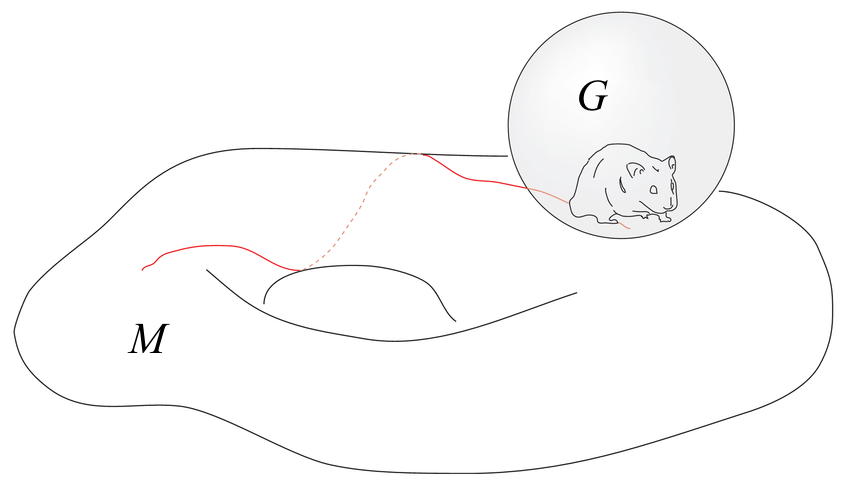
\includegraphics[scale=0.2]{figures/development.png}
    \caption{Development of a path in $(M,\omega)$ to a path in $(G,\theta_G)$. As the mouse follows the path in $M$, the contact point traces out a developed path in $G$.}
    \label{fig:development} 
\end{figure}


\begin{thm}[Generalized Fundamental Theorem]\label{prop generalization of fundamental thm}
    The Fundamental Theorem~\ref{thm 7.14 Sharpe fundamental global} continues to hold for maps $f:M\to G$ if $G$ is replaced with any connected manifold with a $1$-form $\eta$ satisfying all $3$ conditions in Theorem~\ref{thm 8.7 Sharpe}. Namely, let $M$ be connected and simply connected, let $\omega\in\Omega^1(M;\frakg)$, and $x_0\in M$. Then for each $g_0\in G$ there exists a unique smooth map $f:M\to G$ such that $f(x_0)=g_0$ and $f^\ast\eta=\omega$ iff $\omega$ satisfies the structure equation.
\end{thm}
\begin{proof}
    Local solutions exist by the same argument as in the Local Fundamental Theorem~\ref{thm 6.1 Sharpe fundamental local}. The main ingredient leading to global existence is the ability to develop $\omega$ along arbitrary paths (thus lifting those paths to $G$) with the help of the completeness of $\eta$.

    Let $\gamma:I\to M$ be a path and $g_0\in G$ a point. We would like to show that the form $\gamma^\ast \omega\in \Omega^1(I;\frakg)$ can be developed to give a path $\wt\gamma$ in $G$ starting at $g_0$ such that $\eta(\dot{\tilde\gamma}(t))=\omega(\dot\gamma(t))$. The completeness of $\eta$ will be crucial in constructing $\wt\gamma$.

    \emph{Step 1:} construct \emph{exponential maps} on $G$. At every point $g\in G$, we define the exponential map $\exp_g:\frakg\to G$ using the flows of the constant vector fields $\eta^{-1}(A)$, $A\in\frakg$. Let us denote the flow of $\eta^{-1}(A)$ by $F^A_t$, and put 
    \[\exp_g(A)\coloneqq F^A_1(g),\quad g\in G,\;A\in\frakg.\]
    This is well-defined because the flows $F^A_t$ are complete by assumption. This map is smooth by the same exact argument that we will use for the actual exponential map in Proposition~\ref{prop properties of exp}(a). Its differential at the origin is easy to compute. We identify $\T_0\frakg$ with $\frakg$. Let $X_g\in T_g G$ and let $A=\eta(X_g)$ (recall that this correspondence $\T_g G\to \frakg$ is bijective), so that the constant vector field $\eta^{-1}(A)$ has value $X_g$ at $g$. Then 
    \[(\exp_g)_{\ast 0}(A)=\restr{\frac{\dd}{\dd t}}{t=0}F^A_t(g)=\eta^{-1}(A)_g=X_g,\]
    in other words $(\exp_g)_{\ast 0}=\eta^{-1}_g$, which is an isomorphism. Thus, $\exp_g$ is a local diffeomorphism mapping some $0$-neighborhood $U\subset \frakg$ diffeomorphically to an open neighborhood $V\subset G$ of $g$. We will call such sets $V$ \emph{exponential neighborhoods}.

    % \emph{Step 3:} approximate paths in $G$ with ``piecewise-linear'' ones. Consider any path $\wt\gamma:I\to G$ and break it up into a finite (by compactness of $I$) collection of segments each of which is contained in an exponential neighborhood $V_i$ of a point $g_i\in \gamma(I)\subset G$. We can assume that $V_i$ is contractible, so any smooth path $\wt\gamma_i:[a_i,a_{i+1}]\to V_i$ passing through $g_i$ is homotopic, with a fixed value $g_i$, to a path of the form 
    % \[\sigma_i=\exp_{g_i}(A_i t),\quad A_i\in\frakg.\]
    % Then along $\sigma_i$ the value of $\omega$ is constant: $\omega(\dot\sigma_i)=A_i$.  All together, $\wt\gamma$ is homotopic to a piecewise smooth path $\sigma:I\to G$ such that $\sigma(I)\subset \bigcup_i V_i$ and $\omega(\dot\sigma)$ is piecewise-constant. We can also assume that $V_i$ is mapped by $\exp_{g_i}^{-1}$ to a ball of a fixed radius $\epsilon>0$ in $\frakg$. 
    
    % \emph{Step 4:} construct the development of $\sigma$. By assumption, the constant vector fields $\omega^{-1}(A_i)$ are complete and the segments $\sigma_i$ are integral curves for them. Thus, given a starting point $g_0$, we can define the ``development'' $\wt\sigma$ of $\eta$ along $\sigma$ as the path obtained by applying, sequentially, the flows $F^{A_i}_t$ for $t\in [a_i,a_{i+1}]$. 
    
    % \emph{Step 5:} show invariance of the endpoint. Different choices of the approximating path $\sigma$ are homotopic to each other. Let $h:I\times I\to G$ be such a homotopy. The pullback $h^\ast \omega\in \Omega^1(I^2;\frakg)$ still satisfies the structure equation, so by the same argument as in Theorem~\ref{thm 7.7 Sharpe}, the endpoint $\wt\sigma(1)$ is independent of the choice of $\sigma$. Since $\epsilon$ can be made arbitrarily small, by continuity the endpoint also remains stationary during homotopic deformations of $\gamma$ itself (with fixed endpoints).

    \emph{Step 2:} construct ``piecewise-linear'' developments of $1$-forms. Any $1$-form $\xi(t)\dd t\in\Omega^1(I;\frakg)$ can be approximated (under some supremum norm on $\frakg$-valued functions) by a $1$-form $\xi_c(t)\dd t$ such that $\xi_c:I\to \frakg$ is piecewise-constant, $\xi_c(t)=A_i$, $t\in[a_i,a_{i+1}]$. Each constant segment of this $1$-form can be developed to a path in $G$ from any given starting point $g_i$, using the flow $\Fl^{A_i}_t$:
    \[\sigma_i(t)=\exp_{g_i}(A_i t).\]
    We do this inductively, starting with the given $g_0\in G$ and letting $g_{i+1}=\exp_{g_i}(A_i (a_{i+1}-a_i))$, see Figure~\ref{fig:develop}. By refining the approximation we can guarantee that the developed segments stay within exponential neighborhoods of their starting points, and that the images of those neighborhoods in $\frakg$ are balls of fixed radius $\epsilon>0$. This allows us to lift any homotopy that deforms $\xi_c$ into an approximation with even smaller $\epsilon$ to a homotopy $h$ of the developed path in $G$ (by lifting it inside each exponential neighborhood separately). The pullback $h^\ast \eta\in \Omega^1(I^2;\frakg)$ still satisfies the structure equation, so by the same argument as in Theorem~\ref{thm 7.7 Sharpe}, the endpoint $\sigma(1)$ is independent of the choice of approximation.

    \emph{Step 3:} develop $\omega$ along paths in $M$ to paths in $G$. For any path $\gamma:I\to M$, we can develop approximations of the $1$-form $\gamma^\ast \omega$ from any starting point $g_0\in G$, getting a unique endpoint that doesn't depend on the approximation. Since $\omega$ satisfies the structure equation, the endpoint is \emph{also} independent of homotopic deformations of $\gamma$ itself (with fixed endpoints). By replacing the interval $I$ with $[0,t]$, we define not just the endpoint but the whole development $\wt\gamma(t)$ of $\omega$ along $\gamma$. It has to be smooth because $\wt\gamma^\ast \eta$ is uniformly approximated by developable $1$-forms whose limit is $\gamma^\ast\omega$, and local primitives of the latter are smooth by the argument in the local Fundamental Theorem.

    \emph{Step 4:} construct $f$. Now take our $1$-form $\eta$ and define its primitive $f:M\to G$ subject to the condition $f(x_0)=g_0$ as follows. For each $x\in M$, we pick a path $\gamma:x_0\leadsto x$, develop $\gamma^\ast\eta$ to $\wt\gamma$ as above starting at $g_0$ and put $f(x)\coloneqq \wt\sigma(1)$. Since $M$ is simply connected, all choices of $\gamma$ are homotopic to each other, hence their piecewise smooth approximations are also homotopic, and $f(x)$ is independent of these choices. By the same argument as in Theorem~\ref{thm 7.14 Sharpe fundamental global}, locally near $x$, $f(x)$ has to coincide with the unique local primitive, and hence is smooth and $f^\ast\eta=\omega$. Global uniqueness follows from local uniqueness.
\end{proof}

\begin{figure}[tp]
    \def\svgwidth{0.5\linewidth}
    \centering
    \import{figures/}{develop.pdf_tex}
    % 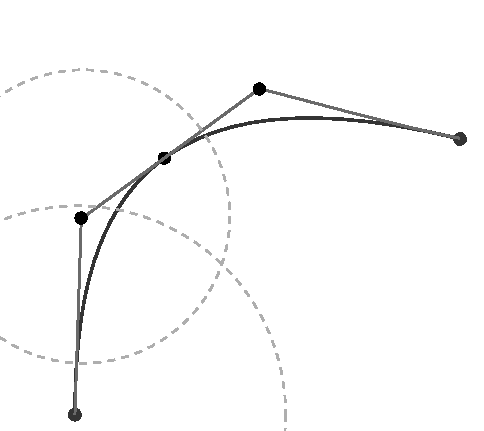
\includegraphics[scale=0.5]{figures/develop.pdf}
    \caption{Piecewise-linear approximations to a development.\label{fig:develop}}
\end{figure}

\begin{proof}[Proof of Theorem~\ref{thm 8.7 Sharpe}]
    First we discuss the case of simply connected $M$, so that $G=M$. This case involves five steps. First we construct a map $f:M\to \GL(\frakg)$ that will eventually be given by $f(g)=\Ad_g$. The second step constructs a map $m:M\times M\to M$ satisfying the conditions $m(e,e)=e$ and $m^\ast \eta=(\pr_2^\ast f)^{-1} \circ \pr_1^\ast\eta+\pr_2^\ast\eta$ (see (\ref{eq MC form under m})). The third step shows that $f$ is a homomorphism w.r.t.\ the multiplication $m$. The fourth shows that $m$ is associative. The fifth step constructs a map $i:M\to M$ and shows that it is the inversion w.r.t.\ $m$.

    \emph{Step 1.} Corollary~\ref{cor 5.3 Sharpe} shows that any map $f:M\to \Aut(\frakg)\subset \GL(\frakg)$ should have logarithmic derivative $\ad_{\eta}\in \frakgl(\frakg)$ and satisfy $f(e)=e$. Thus the form $\eta$ will determine $f$, provided $\omega=\ad_\eta$ is integrable (i.e., satisfies the structure equation). But
    \[\dd\omega+\frac12[\omega,\omega]=\ad_{\dd\eta}+\frac12[\ad_\eta,\ad_\eta]=\ad_{\dd\eta+\frac12[\eta,\eta]}=0,\]
    and since $M$ is simply connected, it follows from the Fundamental Theorem~\ref{thm 7.14 Sharpe fundamental global} that $\eta$ is the logarithmic derivative of a unique map $f:M\to \GL(\frakg)$ satisfying $f(e)=e$. In particular, $\dd f=f\cdot \ad_\eta$, where the product on the right is the composition of elements in $\frakgl(\frakg)$ as linear maps.

    \emph{Step 2.} We construct the multiplication map. Any potential multiplication map $m:M\times M\to M$ should have logarithmic derivative at $(x,y)\in M\times M$ given by the analog of (\ref{eq MC form under m}):
    \[\omega=\pr_1^\ast (f(y)^{-1}\eta)+\pr_2^\ast\eta=(\pr_2^\ast f^{-1})\pr_1^\ast\eta+\pr_2^\ast\eta.\]
    Thus the form $\eta$ will determine $m$, provided $\omega$ is integrable. Now one checks that $\dd\omega+\frac12[\omega,\omega]=0$ by a lengthy direct substitution and using the structure equation on $\eta$, the equality $\dd (f^{-1})=-\ad_\eta\circ f^{-1}$, and the commutativity of the wedge product of $\frakg$-valued $1$-forms. Since $M$ is simply connected, the generalized Fundamental Theorem~\ref{prop generalization of fundamental thm} shows that $\omega$ is the log-derivative of a unique map $m:M\times M\to M$ satisfying $m(e,e)=e$.

    \emph{Step 3.} We show that $f:M\to \GL(\frakg)$ is a homomorphism w.r.t.\ $m$ in the sense that $f(m(x,y))=f(x)f(y)$ for all $x,y\in M$. We shall prove the commutativity of the square consisting of $m,m_{\GL},f$, and $f\times f$:
    \[m_{\GL}\circ (f\times f)=f\circ m.\]
    It is clear that this square commutes at $(e,e)$. Since $M$ is connected it suffices to show that the Maurer-Cartan form $\theta_{\GL}$ on $\GL(\frakg)$ pulls back to the same form on $M\times M$ along the two possible routes. Indeed, $\theta_{\GL(\frakg)}$ trivializes the tangent bundle of $\GL(\frakg)$ and thus its composition with the derivative of any map identifies that derivative, and hence the map itself, up to a constant. Thus, we must show that two logarithmic derivatives coincide:
    \[(f\circ m)^\ast\theta_{\GL}=(m_{\GL}\circ (f\times f))^\ast \theta_{\GL}.\]
    Once again, a lengthy substitution of $m^\ast\eta=\pr_2^\ast(f^{-1}(\pr_1^\ast\eta))+\pr_2^\ast\eta$ and $m_{\GL}^\ast\theta_{\GL}=\pr_2^\ast \Ad^{-1}_{\pr_1^\ast\theta_{\GL}}+\pr_2^\ast \theta_{\GL}$ confirms that the above identity is true.

    \emph{Step 4}. Now we need to show that $m$ is associative. This is equivalent to the commutativity of yet another square:
    \[m\circ (m\times \id)=m\circ (\id\times m).\]
    Again, this diagram clearly commutes at $(e,e,e)$, and since $M$ is connected, it suffices to show that the form $\eta$ on $M$ pulls back to the same form on $M\times M\times M$ along the two possible routes. Another lengthy substitution using the same identities verifies that this holds.

    \emph{Step 5.} Finally we construct an inversion map. Another trivial exercise is to check using (\ref{eq MC form under i}) that any inversion map $i:M\to M$ must have ``log-derivative'' (pullback of $\omega$) given by the prototype of ``$-\Ad_x\circ \eta(X)$'':
    \[\omega_x(X)=-(f\eta)(X),\quad x\in M,X\in \T_x M.\]
    Thus the form $\eta$ will determine $i$, provided we can show that $-f\eta$ is integrable. But since
    \[\dd\omega+\frac12[\omega,\omega]=-(\dd f)\eta -f\dd \eta+\frac12 f[\eta,\eta]=-f\ad_\eta\eta +f[\eta,\eta]=0\]
    and $M$ is simply connected, it folows from the generalized Fundamental Theorem~\ref{prop generalization of fundamental thm} that $\omega$ is the pullback of $\eta$ by a unique map $i:M\to M$ satisfying $i(e)=e$. However, we must still verify that $i$ is the inverse map, i.e., that $m(i(x),x)=e$. This identity can be written as the composition
    \[m\circ(i\times\id)\circ\Delta=e\in M,\]
    where $\Delta:M\to M\times M$ is the diagonal map $\Delta(x)=(x,x)$. Since $M$ is connected, it suffices to show that the form $\eta$ on $M$ pulls back to the same form on $M$ along the two possible routes. Since it obviously pulls back to $0$ via the right hand side, we must show that $(m\circ(i\times\id)\circ\Delta)^\ast\eta=0$. As in the previous steps, a lengthy substitution using the formula for $m^\ast\eta$ verifies this identity. Thus, $i$ is an inverse for $m$.

    \emph{The case $\pi_1(M)\neq 0$.} Here the form $\eta$ on $M$ lifts to the form $\pi^\ast \eta$ on the universal cover $G$. Clearly it satisfies the same three conditions on $G$ that $\eta$ does on $M$. Then our proof applies to the pair $(G,\pi^\ast\eta)$ and we see that for any fixed choice $e\in G$ there is a Lie group structure on $G$ for which $e$ is the identity and $\pi^\ast\eta$ is the Maurer-Cartan form. Its uniqueness follows from Theorem~\ref{thm second principle}: the unique isomorphism between any two group structures on $G$ is provided by the identity map. By Proposition~\ref{prop 8.1 Sharpe}, there is a unique injective homomorphism $\wt{\Phi}:\Aut(\pi)\to G$ satisfying $\wt{\Phi}(A)g=A(g)$ for all deck transformations $A\in \Aut(\pi)$. Thus the group of deck transformations is identified with the period group, a discrete subgroup $\Gamma\subset G$.
\end{proof}

\begin{rem}
    \begin{enumerate}
        \item Dropping the completeness condition (iii) in Theorem~\ref{thm 8.7 Sharpe} still leads to a manifold with a structure of a \emph{local Lie group}, for example, an open subset of a Lie group.
        \item If we drop condition (i) (the structure equation), we are left with what may be regarded as a ``deformation'' of a Lie group. We will later see that this produces a Cartan geometry with nonzero curvature.
        \item Except in special cases, we cannot weaken the isomorphism condition (ii) to $\eta_x$ being merely an injection for all $x\in M$ and still expect to obtain a discrete monodromy group. Therefore, this condition will remain a crucial part of the definition of a Cartan geometry.
    \end{enumerate}
\end{rem}

Theorem~\ref{thm 8.7 Sharpe} provides an easy proof of the existence and uniqueness of universal covering groups (Theorem~\ref{thm 7.7. Lee covering group}).

\begin{proof}[Proof of Theorem~\ref{thm 7.7. Lee covering group}]
    Let the universal covering map be $\pi:\wt{G}\to G$. First note that if a Lie group structure on $\wt{G}$ exists, then the Maurer-Cartan form on $\wt{G}$ is $\pi^\ast \theta_G$. Thus we are led to define $\eta=\pi^\ast\theta_G$ on $\wt{G}$. This form satisfies the structure equation by naturality of exterior derivatives and Lie brackets. Since $\pi$ is a local diffeomorphism, not only is $\eta$ an isomorphism on each fiber, but also $\eta$ is complete, since integral curves for $\theta_G$ on $G$ will lift to integral curves for $\eta$ on $\wt{G}$. By Theorem~\ref{thm 8.7 Sharpe}, given $\wt{e}\in \pi^{-1}(e)$, $\wt{G}$ has a unique Lie group structure with $\wt e$ as the identity and for which $\eta$ is the Maurer-Cartan form. By Theorem~\ref{thm 6.1 Sharpe fundamental local}, $\pi$ is the unique map $(\wt{G},\wt{e})\to (G,e)$ pulling back $\eta$ from $\theta_G$, and then by Theorem~\ref{thm second principle} it must be a homomorphism.
\end{proof}

If one assumes Theorem~\ref{thm 7.7. Lee covering group} to be known (via our original proof), then a much shorter proof of Theorem~\ref{thm 8.7 Sharpe} can be given based on the Ehresmann Fibration Theorem. We have avoided this proof due to the value of the concepts developed over the course of the longer proof.

\begin{proof}[Shorter proof of Theorem~\ref{thm 8.7 Sharpe} {{\cite[Thm.~2.8]{McKayCartan}}}]
    Consider again the Pfaffian system on $M\times G$ spanned by the (components of the) $1$-form $\pr_M^\ast\eta-\pr_G^\ast\theta_G$. By the proof of the local Fundamental Theorem~\ref{thm 6.1 Sharpe fundamental local}, it is integrable and the leaves of the integral foliation are locally graphs of maps $M\to G$. Moreover, since both $\eta$ and $\theta_G$ are fiberwise isomorphisms, these maps are local diffeomorphisms that pull $\theta_G$ back to $\eta$. 
    
    Let $S$ be a leaf of the foliation through some point $(m_0,e)$. Take a constant vector field $\eta^{-1}(A)$ on $G$ for some $A\in\frakg$. The vector field $X\coloneqq (\eta^{-1}(A),A_\rmL)$ on $M\times G$ is tangent to $S$ since $\restr{\pr_M^\ast\eta}{S}=\restr{\pr^\ast_G\theta_G}{S}$. We can simultaneously consider the integral curve $\gamma_M$ of $\eta^{-1}(A)$ through $m_0$ and $\gamma_G$ the integral curve of $A_\rmL$ through $e$. We see that the integral curve $\gamma$ of $X$ through $(m_0,e)\in M\times G$ lies in $S$ and projects onto $\gamma_M$ and $\gamma_G$, respectively. As long as both of the latter curves exist, $\gamma$ exists as well. This means that $\eta^{-1}(A)$ and $A_\rmL$ can be lifted to a unique complete vector field on $S$. Since these vector fields span the tangent bundles, we can now use the Ehresmann Fibration Theorem in the form of Corollary~\ref{thm Ehresmann vector fields} to conclude that $S$ is a fiber bundle over both $M$ and $G$. All three have the same dimension, therefore $S$ is actually a covering space of both $G$ and $M$. 
    
    By an extension of the same lifting argument, we can now replace $S$ with the universal covering space $\wt M$ of $M$. The resulting covering map $D\coloneqq \wt M\to G$ is called a \emph{developing map}. \index{Developing map}
    By Theorem~\ref{thm 7.7. Lee covering group}, $\wt M$ has a unique Lie group structure (for each choice of identity) that turns $D$ into a local Lie group isomorphism. The deck transformations of $\wt M$ preserve the pullback of $\eta$. But the developing map might not be invariant under the deck transformations. Each deck transformation $a\in \Aut(\wt{M})\cong \pi_1(M)$ takes $(m_0,e)$ to some $(m,g)$. By uniqueness of leaves of the foliation, the entire transformation must be simply the left translation $\rmL_g$ acting on the $G$-component, as asserted.
\end{proof}

In this picture, developments of $\eta$ correspond to unique liftings of curves in $M$ to curves in $\wt{M}$ and then projection to $G$ via the developing map.






\section{One-parameter subgroups}


\begin{lem}\label{3972}
    If $G$ is a Lie group and $\frakh\subset \Lief G=\T_e G$ is a Lie subalgebra, then the subset $D_\rmL=\bigcup_g (\rmL_g)_{\ast e}\frakh\subset \T G=G\cdot \frakh$ is a left-invariant involutive distribution. Similarly, $D_\rmR=\frakh\cdot G$ is a right-invariant involutive distribution. 
\end{lem}
\begin{proof}
    It is sufficient to show this for the left-invariant case. Let $D=D_\rmL$. For each $g\in G$, $(\rmL_g)_{\ast e}$ is an isomorphism, therefore $D_g$ is of constant rank $\dim \frakh$ and the distribution is obviously left-invariant. Any basis of left-invariant vector fields on $G$ forms a smooth frame for $D$, so $D$ is smooth. Moreover, $D$ is involutive because such a frame is closed under the Lie bracket.
\end{proof}

The Frobenius theorem now gives us the first the first ``enhancement'' result about Lie subgroups. Even though by definition they are only required to be immersed (which means that their topology can differ drastically from the subspace topology), the following theorem shows that they are in fact weakly embedded (initial).

\begin{thm}[Lie subgroups are weakly embedded {{\cite[Thm.~19.25]{Lee}}}]\label{thm 19.25 Lee}
    Every Lie subgroup is an integral manifold of an involutive distribution, and therefore is a weakly embedded submanifold.
\end{thm}
\begin{proof}
    Let $H\subset G$ be a Lie subgroup. Then $\Lief H$ is canonically isomorphic to the Lie subalgebra $i_\ast(\Lief H)\subset \Lief G$, where $i:H\hookrightarrow G$ is the inclusion. Let $D\subset \T G$ be the left-invariant involutive distribution corresponding to $\frakh$ as in Lemma~\ref{3972}. It follows that $\T_hH=D_h$, so $H$ is an integral manifold of $D$ and is weakly embedded by Theorem~\ref{thm 19.17 Lee}.
\end{proof}

Recall from Theorems~\ref{thm 5.31 Lee} and \ref{thm 5.32 Lee} that while an immersed submanifold can have its topology (and, in a uniquely corresponding way, smooth structure) adjusted in many ways while still remaining immersed, a weakly embedded submanifold has \emph{only one} topology and smooth structure under which it's still immersed. This means that the topology of an immersed Lie subgroup is much more rigid than we originally assumed in the definition.

\begin{rem}
    Note that this does not \emph{yet} allow us to completely drop the assumption of any smooth structure in the definition of a Lie subgroup. A weakly embedded submanifold still needs to be immersed by definition, which presumes a predefined smooth structure on it. We have only shown that this smooth structure is unique. The existence of a smooth structure on an arbitrary path-connected subgroup of a Lie group is a much deeper result which we will demonstrate in \S\ref{sec: Yamabe's theorem}
\end{rem}

\begin{thm}[{{\cite[Thm.~19.26]{Lee}}}] Let $G$ be a Lie group and $\frakg=\Lief G$ its Lie algebra. If $\frakh\subset \frakg$ is a Lie subalgebra, then there is a unique connected immersed Lie subgroup of $G$ whose Lie algebra is $\frakh$.
\end{thm}
\begin{proof}
    Let $D\subset \T G$ be the involutive left-invariant distribution corresponding to $\frakh$. We now use the global Frobenius theorem to introduce the foliation $\calH$ determined by $D$, and for any $g\in G$, let $\calH_g$ be the leaf containing $g$. Since $D$ is left-invariant, it follows that left translations take leaves to leaves: $\rmL_g(\calH_{g'})=\calH_{gg'}$.

    Define $H=\calH_e$. We will show that $H$ is the desired Lie subgroup. First, it is a subgroup because it is left-invariant: $hh'\in \rmL_h(H)=\calH_h=H$ for all $h,h'\in H$, and similarly $h^{-1}\in H$.

    To show that $H$ is a Lie group we need to show that the map $\mu(h,h')=hh^{\prime -1}$ is smooth as a map $H\times H\to H$. Since $H\times H$ is a submanifold of $G\times G$, it is immediate that $\mu:H\times H\to G$ is smooth. Since $H$ is also weakly embedded by Theorem~\ref{thm 19.17 Lee}, $\mu$ is also smooth as a map into $H$.

    The fact that $H$ is a leaf of $\calH$ implies that the Lie algebra of $H$ is $\frakh$, because $\T_eH=D_e=\frakh$. Now suppose there is another subgroup $\wt{H}$ with the same Lie algebra. By maximality of $H=\calH_e$, we have $\wt H\subset H$. On the other hand, in any flat chart for $D$ containing $e$, $\wt H$ must consist of open subsets of slices. Since the slice containing $e$ is an open subset of $H$, this means that $\wt H$ contains a neighborhood of $e$ in $H$. But every neighborhood of $e$ generates the connected Lie group $H$ by Proposition~\ref{prop 7.14 Lee}, therefore $\wt H=H$.
\end{proof}


\begin{defn}
    A \gls{ops} of a Lie group $G$ is a Lie group homomorphism $\gamma:(\bbR,+)\to G$, i.e.~a complete curve such that $\gamma(0)=e$ and $\gamma(t+s)=\gamma(t)\gamma(s)$.
\end{defn}

Note that a \gls{ops} is \emph{not} a Lie subgroup of $G$, but a specific homomorphism. However the images of these homeomorphisms are weakly embedded by Theorem~\ref{thm 19.25 Lee} can be identified with certain Lie subgroups:

\begin{prop}
    Images of \glspl{ops} in $G$ are precisely the connected Lie subgroups of dimension at most 1. Moreover, every such subgroup is either isomorphic to $\bbR$ or $\bbS^1$, or trivial.
\end{prop}
\begin{proof}
    Every connected Lie subgroup of dimension $1$ is automatically abelian and is the integral curve of the left-invariant vector field corresponding to any nonzero tangent vector to the subgroup at $e$. Such an integral curve defines the required \gls{ops}. The isomorphisms hold because any one-dimensional Lie group is a factor of $\bbR$ (the only simply connected one-dimensional Lie group) by a discrete subgroup, and all such subgroups of $\bbR$ are either trivial or isomorphic to $\bbZ$.
\end{proof}


\begin{thm}[Characterization of one-parameter subgroups]
    The \glspl{ops} of a Lie group $G$ are precisely the maximal integral curves of left-invariant vector fields starting at $e\in G$.
\end{thm}
\begin{proof}
    Given a left-invariant vector field, its integral curve at $e$ will automatically be a \gls{ops} due to the general group property of flows and completeness (or alternatively from the uniqueness of maximal integral curves).

    Conversely, every \gls{ops} $\gamma$ is the integral curve of the left-invariant field $A_\rmL$ whose value at the identity is $A=\dot\gamma(0)\in\Lief G$ because 
    \[\dot\gamma(t)=\restr{\frac{\dd}{\dd s}}{s=0}\rmL_{\gamma(t)}\gamma(s)=\rmL_{\gamma(t)\ast e}A=(A_\rmL)_{\gamma(t)}.\]
\end{proof}

This leads us to yet another common way of defining the Lie algebra of a Lie group.

\paragraph{Construction IV} In summary, there is a natural one-to-one correspondence between elements of the Lie algebra and \glspl{ops}
\[A\in \frakg\cong \fX(G)^G\mapsto \gamma_A(t)=F^A_t(e)\coloneqq \Fl^{A_\rmL}_t(e).\]
We say that $\gamma_A$ is \emph{generated} by $A\in\frakg$. The Lie bracket is recovered as the double derivative of the group commutator
\[[A,B]=\restr{\frac{\dd}{\dd t}\frac{\dd}{\dd s}}{t=s=0}\gamma_A(t)\gamma_B(s)\gamma_A(t)^{-1}\gamma_B(s)^{-1}.\]

The following is a well known fact of linear algebra.

\begin{prop}
    For $A\in \mathfrak{gl}_n(\bbK)$, the \gls{ops} generated by it in $\GL_n(\bbK)$ is
    \[\gamma_A(t)=\rme^{tA}=\exp tA.\]
\end{prop}
\begin{cor}
    Uniqueness of integral curves implies that the \glspl{ops} of a Lie subgroup $H< G$ are exactly the ones generated by $\frakh < \frakg$. Therefore in \emph{all} matrix groups the \glspl{ops} are given by exponentials.
\end{cor}

\begin{prop}[{{\cite[Prop.~20.3]{Lee}}}]\label{prop 20.3 Lee}
    If $H< G$ is a Lie subgroup, then the \glspl{ops} of $H$ are precisely those \glspl{ops} of $G$ that are generated by elements of $\frakh=\T_e H$.
\end{prop}
\begin{proof}
    Clearly any \gls{ops} $\gamma:\bbR\to H$ can also be viewed as a \gls{ops} of $G$ (by composing with the inclusion map) which satisfies $\dot\gamma(0)\in \T_e H$.

    Conversely, a \gls{ops} of $G$ generated by an element of $\T_e H$ must coincide with the analogous \gls{ops} of $H$ by uniqueness of maximal integral curves.
\end{proof}







\section{Exponential map}


\begin{defn}[Exponential map]\index{Exponential map}
    Given a Lie group $G$ with Lie algebra $\frakg=\Lief G$, the exponential map $\exp:\frakg\to G$ assigns to each $A\in \frakg$ the group element
    \[\exp A=\gamma_A(1),\]
    where $\gamma_A$ is the \gls{ops} generated by $A$. As a consequence, the \gls{ops} generated by $A$ can be written as \[\gamma_A(t)=\gamma_{tA}(1)=\exp tA=\rme^{tA}.\]
    (While we use the notations $\exp A$ and $\rme^A$ interchangeably, the exponential map is related to the Euler number only in the case of linear Lie groups.)
\end{defn}

When multiple groups are involved, we will sometimes specify the group to which the exponential map belongs by writing, for example, $\exp_G$.

\begin{prop}\label{prop properties of exp} The exponential map $\exp:\frakg\to G$ has the following properties for all $A\in\frakg$.
\begin{enumerate}[label=(\alph*)]
    \item $\exp$ is smooth.
    \item $\rme^{sA}\rme^{tA}=\rme^{(s+t)A}$ for $s,t\in\bbR$.
    \item $\left(\rme^A\right)^{-1}=\rme^{-A}$.
    \item $\left(\rme^A\right)^{n}=\rme^{nA}$ for $n\in \bbZ$.
    \item $\exp_{\ast 0}=\id_\frakg$.
    \item $\exp$ restricts to a diffeomorphism from some neighborhood of $0\in \frakg$ to a neighborhood of $e\in G$. Its inverse is often denoted by $\ln$.
    \item $\exp$ is natural: if $H$ is another Lie group with $\frakh=\Lief H$, and $\Phi:G\to H$ is a Lie group homomorphism, then 
    \[\exp_H\circ\Phi_{\ast e}=\Phi\circ \exp_G.\]
    \item The flow $\Fl^{A_\rmL}$ of a left-invariant vector field $A_\rmL\in \fX(G)^G$, $(A_\rmL)_e=A$, is given by $F_t=\rmR_{\rme^{tA}}$.
\end{enumerate}
\end{prop}
\begin{proof}
    (a) We need to show that the flow $F^A$ of a vector field varies smoothly with $A$. This is a situation not covered by the fundamental theorem of flows, but we can reduce it to that situation by a simple trick. Define a vector field $\Xi\in\fX(G\times\frakg)$ by
    \[\Xi_{(g,A)}=((A_\rmL)_g,0)\in \T_gG\oplus \T_A \frakg.\]
    This is a smooth vector field because it acts on functions by differentiating them along $A_\rmL$. It is easy to verify that the flow $F^\Xi$ is given by
    \[F^\Xi_t(g,A)=\left(\Fl^{A_\rmL}(g,t),A\right).\]
    By the fundamental Theorem~\ref{thm fundamental of flows} of flows, $F^\Xi$ is smooth. Since $\exp A=\pr_1\left(F^\Xi_1(e,A)\right)$, where $\pr_1:G\times\frakg\to G$ is the projection, it follows that $\exp$ is smooth.

    (b-d) follow trivially from the fact that $\exp(tA)$ is a \gls{ops}.
    
    To show (e) we compute
    \[\exp_{\ast 0}A=\restr{\frac{\dd}{\dd t}}{t=0}F_t^{A}(e)=A,\]
    i.e.~$\exp_{\ast 0}$ coincides with the natural isomorphism $\fX(G)^G\cong \T_e G$. Then by the \gls{inmt}, $\exp$ is a local diffeomorphism and (f) follows.

    (g) follows from the naturality of flows of vector fields:
    \[\Fl^{\Phi_\ast A}_t\circ \Phi=\Phi\circ \Fl^{A}_t,\]
    and setting $t=1$ and evaluating at the identity yields (g).

    (h) was already proven in Lemma~\ref{lem 471841}.
\end{proof}

\begin{rem}
    The naturality of $\exp$ implies, in particular, that $g\rme^{tA}g^{-1}=\rme^{t\Ad_g A}$. This confirms the intuitive picture that conjugate subgroups are generated by conjugate elements of the Lie algebra. For example, on $\SO_3$, let $H\cong\SO_2$ be the \gls{ops} of rotations about the $z$-axis. Then if $g$ is a rotation which maps $\bf{e}_3=(0,0,1)$ to some vector $\bf{n}$, then the subgroup of rotations about $\bf{n}$ is $gHg^{-1}$ and is generated by 
    \[A_{\bf{n}}=A_{g\bf{n}}=\Ad_g A_{\bf{e}_3}=gA_{\bf{e}_3} g^{-1},\] 
    where $A_{\bf{e}_3}$ generates rotations about $\bf{e}_3$, cf.\ Example~\ref{example su2 and so3}.
\end{rem}
\begin{cor}
    The identity component $G_0$ is generated by $\exp(U)$ for any neighborhood $U$ of the origin $0\in\frakg$.
\end{cor}
 

\begin{rem}
    The inverse of the exponential map, $\ln$ (logarithm), provides a \emph{canonical local chart} at $e\in G$. This is a special property of Lie groups that we will use to much benefit. We will call this chart the \emph{logarithmic coordinates} on $G$.
\end{rem}


\begin{prop}\label{prop 5.4.5 RS1 ker(Ad) and ker(ad)}
    The kernels of the adjoint representations of $G$ and $\frakg$ are given by the centralizer of the identity component and the center of the Lie algebra, respectively:
    \[\ker \Ad=\rmC_G(G_0),\quad \ker \ad=\frakz(\frakg).\]
    In particular, the \emph{adjoint group of $G$} is \index{Adjoint group}
    \[\Ad(G)\cong G\slash \rmC_G(G_0),\quad \ad(\frakg)\cong \frakg\slash \frakz(\frakg).\]
\end{prop}
\begin{proof}
    The statement $\ker\ad=\frakz(\frakg)$ is obvious. Since for $g\in \rmC_G(G_0)$ there holds $\restr{\Adg_g}{G_0}=\id_{G_0}$ and since $(\id_G)_{\ast e}=\id_\frakg$, we obtain $\rmC_G(G_0)\subset \ker\Ad$. Conversely, if $g\in G$ satisfies $\Ad_g=\id_\frakg$. The naturality of the exponential map implies 
    \[\rme^A=\rme^{\Ad_g A}=\Adg_g(\rme^A)\text{ for all }A\in\frakg.\]
    That is, $g$ commutes with all elements of $\exp(\frakg)$. Since $\exp(\frakg)$ generates $G_0$, we conclude $\ker\Ad\subset \rmC_G(G_0)$.
\end{proof}

Similarly, for the coadjoint representation we have
\[\ker \Ad^\ast=\rmC_G(G_0),\quad \ker\ad^\ast=\frakz(\frakg).\]

\begin{prop}\label{prop 20.9 Lee}
    If $H\subset G$ is a Lie subgroup, then the exponential map of $H$ coincides with the restriction of the exponential map of $G$, and 
    \[\Lief H=\{A\in\Lief G: \exp(tA)\in H \text{ for all } t\in \bbR\}.\]
\end{prop}
\begin{proof}
    The fact that $\exp_H=\restr{\exp_G}{\frakh}$ follows immediately from Proposition~\ref{prop 20.3 Lee}.

    Next assume that $\rme^{tA}\in H$ for all $t$. Since $H$ is weakly embedded in $G$ by Theorem~\ref{thm 19.25 Lee}, it follows that the curve $t\mapsto \rme^{tA}$ is smooth as a map into $H$, and thus $A=\dot\gamma(0)\in \T_eH$. Conversely, if $A\in \T_e H$ then Proposition~\ref{prop 20.3 Lee} implies that $\rme^{tA}\in H$ for all $t$.
\end{proof}


\begin{thm}\label{thm 1.5.2 DK}
    The following formulas hold for all $A\in\frakg,g\in G$:
    \begin{enumerate}[label=(\alph*)]
        \item $\Ad_{\rme^A}=\rme^{\ad_A}$.
        \item $\Adg_g \rme^A=\rme^{\Ad_g A}$.
    \end{enumerate}
\end{thm}
\begin{proof}
    For (a) we apply the naturality of $\exp$ (Proposition~\ref{prop properties of exp} (g)) to the homomorphism $\Ad:G\to \GL(\frakg)$, and for (b) we apply it to the homomorphism $\Ad_g:G\to G$.
\end{proof}



\begin{example}
    Recall Corollary~\ref{cor generated homomorphism}, where we showed that Lie group homomorphisms with a simply connected source group are uniquely determined by their derivatives at the identity. The Lie group $\SU_2$, being homeomorphic to the sphere $\bbS^3$, is simply-connected. Therefore, every homomorphism $\phi:\fraksu_2\to\frakg$ into any other Lie algebra $\frakg$ of some Lie group $G$ determines a unique homomorphism $\Phi:\SU_2\to G$. 
    
    On the other hand, from Example~\ref{example su2 and so3}, the homomorphism $\Ad:\SU_2\to \SO_3(\bbR)$ is a double covering map since $\ker\Ad=\{\pm \rmI\}$, thus $\SO_3(\bbR)$ doesn't satisfy the condition on the domain group for the same theorem, and it must be possible to find a Lie algebra homomorphism $\psi:\frakso_3(\bbR)\to\frakg$ that doesn't extend to a group homomorphism $\Psi:\SO_3(\bbR)\to G$. Namely, the group homomorphism $\Psi$ exists if and only if 
    \[\exp \psi(A_{2\pi \bf{e}_3})=e_G,\text{ where }A_{2\pi \bf{e}_3}=
    \begin{pmatrix}
        0&0&0\\
        0&0&-2\pi\\
        0&2\pi &0
    \end{pmatrix}.
    \]
    To see this, apply the previous statement to $\phi=\psi\circ\ad$, where we view the adjoint as a map $\ad:\fraksu_2\to\frakso_3(\bbR)$. From this homomorphism, $\Psi$ is determined by $\Phi=\Psi\circ \Ad$; therefore such a homomorphism of Lie groups $\Psi$ exists iff $\Phi(-\rmI)=e_G$, which translates to $\Psi\circ \Ad(-\rmI)=e_G$. Since $\Phi\circ\exp=\exp\circ\phi$ and 
    \[\exp(\rmi \pi\sigma_3)=\exp \begin{pmatrix}
        \rmi \pi&0\\0 &-\rmi \pi
    \end{pmatrix}=-\rmI,\]
    the condition that $\Phi(-\rmI)=e_G$ becomes
    \[e_G=\Phi\circ \exp (\rmi\pi\sigma_3)=\exp\circ\phi (\rmi\pi\sigma_3)=\exp\circ\psi( \ad_{\rmi\pi\sigma_3})=\exp\circ\psi (A_{2\pi \bf{e}_3}),\]
    where at the end we used formula (\ref{eq ad: su2->so3}).
    
    This picture generalizes to all Lie groups. For any group $H$ one can specify a finite set of $A_i\in\frakh$ such that any homomorphism of Lie algebras $\phi:\frakh\to\frakg$ generates a homomorphism of Lie groups $\Phi:H\to G$ iff $\exp\phi(A_i)=e_G$ for all $i$.
\end{example}


\begin{prop}\label{prop exp on abelian groups}
    If $A,B\in\frakg$ commute, i.e.~$[A,B]=0$, then
    \[\rme^A\rme^B=\rme^B\rme^A=\rme^{A+B}.\]
    In particular, if $\frakg$ is abelian, $\exp$ is a Lie group homomorphism from the vector group underlying $\frakg$ to $G$.
\end{prop}
\begin{proof}
    It suffices to show that the curve defined by $\gamma(t)=\rme^{tA}\rme^{tB}$ coincides with the integral curve generated by $A+B$. Indeed, $\gamma(0)=e$ and we can use the commutation of the flows of the left-invariant fields $A_\rmL$ and $B_\rmL$ to compute the generator. Here we will need the general product rule that holds for maps $f:M_1\times M_2\to N$:
    \[\T_{(m_1,m_2)}f(A_1,A_2)=\T_{m_1}f_{m_2}(A_1)+\T_{m_2}f_{m_1}(A_2)\]
    where $f_{m_1}:M_2\to N$ and $f_{m_2}:M_1\to N$ are the partial mappings. In particular, if $M_1=M_2\cong \bbR$ then we have the ``product rule'' for derivatives along the diagonal:
    \[\restr{\frac{\dd}{\dd t}}{t}\varphi(t,t)=\restr{\frac{\dd}{\dd s}}{s=t}\varphi(s,t)+\restr{\frac{\dd}{\dd s}}{s=t}\varphi(t,s).\]
    Applying this to $\gamma$ we get (using $F^A$ for the flow of $A_\rmL$)
    \begin{multline}
        \dot\gamma(0)=\restr{\frac{\dd}{\dd t}}{t=0} \Fl^{B}_t\circ \Fl^{A}_t (e)=\restr{\frac{\dd}{\dd s}}{s=0}\Fl^{B}_{s}(e)+\restr{\frac{\dd}{\dd s}}{s=0}\Fl^{A}_{s}(e)=B+A.
    \end{multline}
\end{proof}

When the elements do not commute, the following two propositions provide an approximate formula.

\begin{prop}[{{\cite[Prop.~20.10]{Lee}}}]\label{prop 20.10 Lee}
    For any $A,B\in\frakg=\Lief G$, there is a smooth function $Z:(-\epsilon,\epsilon)\to \frakg$ for some $\epsilon>0$ such that
    \[\rme^{tA}\rme^{tB}=\exp\left(t(A+B)+t^2Z_2(t)\right)\]
    for all $t\in(-\epsilon,\epsilon)$.
\end{prop}
\begin{proof}
    Since $\exp$ is a local diffeomorphism, there exists an $\epsilon>0$ such that on $(-\epsilon,\epsilon)$ we can consider the smooth map
    \[\varphi(t)=\ln\left(\rme^{tA}\rme^{tB}\right).\]
    Obviously $\varphi(0)=0$ and since the differential of the multiplication map is $(\T_{(e,e)}m)(A,B)=A+B$, we have
    \[\varphi'(0)=\ln_{\ast e}(A+B)=A+B.\]
    By Taylor's theorem $\varphi(t)=t(A+B)+t^2Z_2(t)$ for some smooth $Z_2(t)$.
\end{proof}
The following corollary will be useful in the proof of the Closed Subgroup Theorem~\ref{thm closed subgroup}.
\begin{cor}\label{cor 20.11 Lee}
    Under the hypotheses of the preceding proposition,
    \[\lim_{n\to\infty}\left(\exp \frac{tA}{n}\exp \frac{tB}{n}\right)^n=\exp t(A+B).\]
\end{cor}
\begin{proof}
    We have 
    \begin{multline}
        \left(\exp \frac{tA}{n}\exp \frac{tB}{n}\right)^n=\left(\exp\left(\frac{t}{n}(A+B)+\frac{t^2}{n^2}Z_2\left(\frac{t}{n}\right)\right)\right)^n=\\
        =\exp\left(t(A+B)+\frac{t^2}{n^2}Z_2\left(\frac tn\right)\right).
    \end{multline}
    Taking the limit $n\to\infty$ at fixed $t$ gives the result.
\end{proof}

\begin{prop}
    Under the hypotheses of the preceding proposition, 
    \[\rme^{tA}\rme^{tB}=\exp\left(t(A+B)+\frac{t^2}{2}[A,B]+t^3Z_3(t)\right)\]
    for another smooth map $Z_3:(-\epsilon,\epsilon)\to \frakg$.
\end{prop}
\begin{proof}
    For the function $\varphi$ from the proof of Proposition~\ref{prop 20.10 Lee} we have
    \[\varphi(t)=t(A+B)+t^2Z_2(0)+t^3Z_3(t).\]
    To compute the flow of this vector field we can apply the general Taylor formula for manifolds (\ref{eq:Taylor formula for manifolds}). By an abuse of notation we drop the smooth function $f\in C^\infty(G)$ on which this formula is supposed to act:
    \[\rme^{\varphi(t)}=\restr{\Fl^{A+B+\frac{s}{2}Z_2(0)+\calO(s^2)}_t}{s=t}=1+t(A+B)+\frac{t^2}{2}\left((A+B)^2+2Z_2(0)\right)+\calO(t^3).\]
    On the other hand the Taylor formula for two fields (\ref{eq: Taylor formula for two fields}) gives
    \[\rme^{tA}\rme^{tB}=1+t(A+B)+\frac{t^2}{2}(A^2+2AB+B^2)+\calO(t^3).\]
    We read off $Z_2(0)=[A,B]/2$.
\end{proof}

This gives us a new interpretation of the Lie bracket as the  commutator of infinitesimal flows of left-invariant vector fields (closely connected to formula (\ref{30071})).
\begin{cor}
    By a repeated application of the Taylor series obtained above,
    \[\rme^{tA}\rme^{tB}\rme^{-tA}=\rme^{tB+t^2[A,B]+\calO(t^3)}\]
    and
    \[[\rme^{tA},\rme^{tB}]=\rme^{tA}\rme^{tB}\rme^{-tA}\rme^{-tB}=\rme^{t^2[A,B]+\calO(t^3)}.\]
\end{cor}


\begin{rem}
    By continuing the Taylor expansion endlessly, we can obtain the full formal series for $\ln(\rme^A \rme^B)$ known as the \gls{bch}\index{Equation!Baker-Campbell-Hausdorff} formula. Its special property is that it can be written using only Lie brackets (or adjoints). We will derive it in the next \sect.
\end{rem}










\section{Differential of exp}

\begin{thm}[{{\cite[Thm.~1.5.3]{DK}}}]\label{thm differential of exp}
    For any $A\in\frakg$ the linear mapping $\exp_{\ast A}:\frakg\to \T_{\rme^A} G$ is given by
    \[  \exp_{\ast A}=\left(\rmR_{\rme^A}\right)_{\ast e}\circ \int_0^1 \rme^{s\ad_A}\dd s=\left(\rmL_{\rme^A}\right)_{\ast e}\circ \int_0^1 \rme^{-s\ad_A}\dd s.   \label{eq 1.5.1 DK}\]
\end{thm}
\begin{proof}
    We will provide a simple derivation of this from the Maurer-Cartan equation (\ref{eq Maurer-Cartan}). Let us apply it to the map
    \[g(t,s)=\rme^{t(A+sB)}.\]
    Then we find
    \[\xi=\left(\rmR_g^{-1}\right)_\ast \partial_t g=A+sB, \quad \eta=\left(\rmR_g^{-1}\right)_\ast \partial_s g,\]
    and the Maurer-Cartan equation $\partial_t\eta-\partial_s\xi=[\xi,\eta]$ now reads
    \[\partial_t \eta=B+[A,\eta].\]
    By denoting $\gamma(t)=\eta(t,0)$, we get the differential equation at $s=0$
    \[\dot\gamma(t)=B+[A,\gamma].\label{196}\]
    First we notice that the solution of the homogenous equation $\dot\gamma=[A,\gamma]$ is given by the adjoint curves
    \[\gamma_{\mathrm{hom}}=\Ad_{\rme^{tA}}\gamma_0=\rme^{t\ad_A}\gamma_0.\]
    By Lagrange's method of variation of constants, we look for a solution to (\ref{196}) in the form $\gamma(t)=\rme^{t\ad_A}\zeta(t)$. Plugging this ansatz back into the equation gives
    \[\rme^{t\ad_A}\dot\zeta(t)=B.\]
    The solution of this with $\gamma(0)=0$ is obviously given by
    \[\zeta(t)=\int_0^t \rme^{-s\ad_A}B\dd s.\]
    On the other hand, from the definition of $\gamma$,
    \[\gamma(t)=\left(\rmR_{\rme^{tA}}^{-1}\right)_{\ast \rme^{tA}}\circ \exp_{\ast tA}(tB)\]
    and thus
    \[\exp_{\ast tA}(tB)=\left(\rmL_{\rme^{tA}}\right)_{\ast e}\int_0^t\rme^{-s\ad_A}\dd s\,(tB).\]
    By setting $t=1$ we get the claimed formula. The second version is obtained via the substitution $s=1-s'$ in the integral.
\end{proof}


\begin{rem}[Singular points of $\exp$]
    Since the integral derived above is elementary, the (left or right) logarithmic derivative of $\exp$ at $A\in\frakg$ can be given by the formal series
    \begin{align}
        \delta_A\exp= \left(\rmL_{\rme^{-A}}\right)_{\ast e}\circ \exp_{\ast A}&=\sum_{n=0}^\infty \frac{\left(-\ad_{A}\right)^n}{(n+1)!}=\frac{\rmI-\rme^{-\ad_A}}{\ad_A},\\
        \delta^\rmR_A\exp= \left(\rmR_{\rme^{-A}}\right)_{\ast e}\circ \exp_{\ast A}&=\sum_{n=0}^\infty \frac{\left(\ad_{A}\right)^n}{(n+1)!}=\frac{\rme^{\ad_A}-\rmI}{\ad_A},\label{dexp series}
    \end{align}
    where for non-invertible matrices $\ad_A\in\frakgl(\frakg)$ the series should be taken as the \emph{definition} of this latter expression. Indeed, $\ad_A$ is never invertible because it always contains $A$ itself in its kernel, $\ad_A A=0$. By looking at the location of the zeros of the function $f(z)=(\rme^z-1)/z$, we conclude that the differential $\exp_{\ast A}$ is bijective iff no eigenvalue of $\ad_A$ lies in $2\pi \rmi\bbZ\setminus\{0\}$. Conversely, the singular points of the exponential map are precisely those $A\in \frakg$ such that $\ad_A\in \End(V)$ has an eigenvalue of the form $2\pi \rmi k,$ $k\in\bbZ\setminus\{0\}$.
\end{rem}

\begin{example}[Exponential map of $\SO_3(\bbR)$]
    Recall from Example~\ref{example su2 and so3} that the rotation group $G=\SO_3(\bbR)$ can be parametrized by vectors $\bf{n}\in\bbR^3$ as follows:
    \[R_{\bf{n}}=\rmI+\frac{\sin |\bf{n}|}{|\bf{n}|}A_{\bf{n}}+\frac{1-\cos |\bf{n}|}{|\bf{n}|}A_{\bf{n}}^2,\]
    where $|\bf{n}|=\sqrt{n_1^2+n_2^2+n_3^2}$ is the rotation angle and $A_{\bf n}$ is $|\bf n|$ times the generator of rotations about $\bf n$.

    The conjugacy classes of $\SO_3(\bbR)$ are exactly the spheres $C_{|\bf{n}|}$ of equal rotation angle $0\leq |\bf{n}|\leq \pi$ (except $C_0=\{\rmI\}$). Each conjugacy class in the range $0<|\bf{n}|<\pi$ is diffeomorphic to a sphere, whereas $C_\pi$, the conjugacy class of the matrix $\diag(1,-1,-1)$, is diffeomorphic to $\RP^2$.
    
    Then the singular points of the exponential map are the antisymmetric matrices $A_\omega\in \frakso_3(\bbR)$ with $|\omega|=2\pi$. In this case $\rme^{A_\omega}=\rmI\in \SO_3(\bbR)$. 

    The exponential map is a local diffeomorphism from the ball $|\omega|<2\pi$ onto $\SO_3(\bbR)$ which restricts to a two-fold covering from the punctured ball $0<|\omega|<2\pi$ onto $\SO_3(\bbR)\setminus \{\rmI\}$. The ball $|\omega|<\pi$ is the maximal open subset of $\frakso_3(\bbR)$ on which the exponential mapping is injective; it is mapped diffeomorphically onto the complement in $\SO_3(\bbR)$ of the conjugacy class $C_\pi$.
\end{example}


\begin{example}[Exponential map of $\SL_2(\bbC)$ and $\SU_2(\bbC)$]
If $G=\SL_2(\bbC)$, then its Lie algebra $\frakg=\mathfrak{sl}_2(\bbC)$ consists of traceless matrices
\[A=\begin{pmatrix}
    a&b\\c&-a
\end{pmatrix},\quad \quad a,b,c\in\bbC,\]
and any such matrix satisfies the equation
\[A^2=\lambda^2 \rmI,\quad \lambda=\pm \sqrt{a^2+bc},\]
where $\lambda$ are the eigenvalues of $A$. Due to this the exponential series separates into two sums over odd and even powers, and we get
\[\rme^A=\cosh \lambda \cdot \rmI+\frac{\sinh \lambda}{\lambda}A.\]
Observe that the coefficients here are entire analytic functions of $\lambda^2=a^2+bc$ and hence are entire analytic functions on $\mathfrak{sl}_2(\bbC)$. If $\lambda=0$, we recover the result
\[\rme^A=\rmI+A \; \Leftrightarrow \; A\text{ is nilpotent}\]
(because for $2\times 2$ matrices nilpotency is equivalent to the vanishing of the square). If $\lambda=\i t$ with $t\in \bbR$, the exponential becomes
\[\rme^A=\cos t\cdot \rmI+\frac{\sin t}{t}A.\]
This occurs if $a,b,c\in\bbR$ (which is equivalent to $A\in\mathfrak{sl}_2(\bbR)$) and $a^2+bc<0$, i.e., ``$A$ is in the elliptic domain''. The case $\lambda=\i t$, $t\in\bbR$, also occurs for all matrices of the form
\[A=\begin{pmatrix}
    \i\alpha&\beta\\-\wb{\beta}&-\i\alpha
\end{pmatrix}\in\mathfrak{su}_2.\]
In this case $t=\sqrt{\alpha^2+|\beta|^2}$, which is the Euclidean length of $(\alpha,\beta)\in\bbR\times\bbC\cong \bbR^3$. For $A=\begin{pmatrix}
    0&-1\\1&0
\end{pmatrix}$ we recover the usual notation
\[R(t)=\exp \begin{pmatrix}
    0&-t\\t&0
\end{pmatrix}=\begin{pmatrix}
    \cos t&-\sin t\\\sin t&\cos t
\end{pmatrix}\in\SO_2(\bbR).\]
If $A\in\mathfrak{sl}_2(\bbR)$, then $\rme^A$ has eigenvalues equal to $-1$ iff there is a $k\in\bbZ$ such that $A$ has eigenvalues equal to $\pm\rmi \pi(2k+1)$ (with both signs occurring). This implies that $A$ is diagonalizable over $\bbC$, hence $\rme^A$ is as well, so $\rme^A=-\rmI$. It follows that elements $g\in\SL_2(\bbR)$ that have eigenvalues equal to $-1$ without themselves being equal to $-\rmI$, that is, those $g\in\SL_2(\bbR)$ which are conjugate to $\left(\begin{smallmatrix}
    -1&\pm 1\\0&-1
\end{smallmatrix}\right)$, \emph{are not in the image of $\exp:\mathfrak{sl}_2(\bbR)\to \SL_2(\bbR)$} (and only they aren't).

Defining the algebraic variety in $\frakg$
\[\Sigma_1=\left\{A\in\frakg\mid \det\left(\ad_A^\bbC -2\pi\rmi  \rmI\right)=0\right\},\]
the set of all singular points of the exponential map is $\Sigma=\bigcup_{k\in\bbC\setminus\{0\}} k\Sigma_1$. In the case of $\SL_2(\bbC)$,
\[\Sigma_1=\left\{\begin{pmatrix}
    a&b\\c&-a
\end{pmatrix}\in\mathfrak{sl}_2(\bbC)\mid a^2+bc=-\pi^2\right\}.\]
Thus for $G=\SU_2$,
\[\Sigma_1=\left\{\begin{pmatrix}
    \i\alpha&\beta\\-\wb{\beta}&-\i\alpha
\end{pmatrix}\in\mathfrak{su}_2\mid |\alpha|^2+|\beta|^2=\pi^2\right\},\]
which is a sphere $\bbS^2$ in $\mathfrak{su}_2$ of Euclidean radius $\pi$, and $\exp$ maps the ball $|\alpha|^2+|\beta|^2<\pi^2$ diffeomorphically onto $\SU_2\setminus\{-\rmI\}$. On the other hand, for $G=\SL_2(\bbR)$, the set $\Sigma_1$ is the two-sheeted hyperboloid
\[\Sigma_1=\left\{\begin{pmatrix}
    a&b\\c&-a
\end{pmatrix}\in\mathfrak{sl}_2(\bbR)\mid a^2+bc=-\pi^2\right\},\]
mapped to $\{-\rmI\}$ by the exponential. Here $\exp$ is a diffeomorphism from the set $a^2+bc>-\pi^2$ onto the complement in $\SL_2(\bbR)$ of $\{-\rmI\}$ and the conjugacy classes of $\left(\begin{smallmatrix}
    -1&\pm1\\0&-1
\end{smallmatrix}\right)$, the latter being the elements that are not in the image of $\exp:\mathfrak{sl}_2(\bbR)\to \SL_2(\bbR)$ at all. Note that $\exp_{\fraksl_2}(\bbR)$ is neither open in $\SL_2(\bbR)$ ($-\rmI$ belongs to it, but not as an interior point), nor closed.
\end{example}

\begin{xca}
    Show that the exponential map $\exp:\frakgl_n(\bbC)\to \GL_n(\bbC)$ is surjective. \emph{Hint:} apply the Jordan canonical form to write a conjugate of $A\in\GL_n(\bbC)$ as $D(\rmI+U)$ with $D\in\GL_n(\bbC)$ diagonal and $U$ nilpotent, and use $\ln(\rmI+U)=\sum_{k\geq 0} \frac{(-1)^k}{k+1}U^{k+1}$, which is a terminating series.
\end{xca}





\section{Normal subgroups}

Normal subgroups (those that are invariant under conjugation) play a central role in abstract group theory: they are the only subgroups whose quotients have group structures, and the only subgroups that are kernels of group homomorphisms. First we derive a useful criterion for normality.

\begin{lem}[{{\cite[Lem.~20.23]{Lee}}}]\label{lem 20.23 Lee}
    Let $G$ be a connected Lie group and $H<G$ a connected Lie subgroup. Let $\frakg$ and $\frakh$ denote their respective Lie algebras. Then $H$ is normal in $G$ iff
    \[\rme^A \rme^B \rme^{-A}\in H \text{ for all }A\in \frakg,B\in\frakh.\]
\end{lem}
\begin{proof}
    Since $(\rme^A)^{-1}=\rme^{-A}$, if $H$ is normal, the property in question holds automatically. Conversely, choose open neighborhoods $V\subset \frakg$ of the origin and $U\subset G$ of the identity such that $\exp:V\to U$ is a diffeomorphism. Since the exponential map of $H$ is the restriction of that of $G$, after shrinking $V$ if necessary, we may assume that the restriction of $\exp$ to $V\cap \frakh$ is a diffeomorphism from $V\cap \frakh$ to a neighborhood $U_0$ of the identity in $H$. Shrinking $V$ still further, we may assume that $A\in V$ iff $-A\in V$. Then the assumption implies that $ghg^{-1}\in H$ whenever $g\in U$ and $h\in U_0$.

    Since very element of $H$ can be written as a finite product $h=h_1\cdots h_m$ with $h_1,\ldots, h_m\in U_0$ (Proposition~\ref{prop 7.14 Lee}), it follows that for any $g\in U$ and $h\in H$ we have
    \[ghg^{-1}=gh_1\cdots h_m g^{-1}=(gh_1g^{-1})\cdots (gh_m g^{-1})\in H.\]
    Similarly, any $g\in G$ can be written $g=g_1\cdots g_k$ with $g_1,\ldots, g_k\in U$, so it follows by induction on $k$ that $ghg^{-1}\in H$ for all $g\in G,h\in H$.
\end{proof}


We can now establish a relationship between normal subgroups and ideals of the Lie algebra.

\begin{thm}[Ideals and Normal Subgroups{{\cite[Thm.~20.28]{Lee}}}]\label{thm 20.28 Lee}
    Let $G$ be a connected Lie group, and suppose $H<G$ is a connected Lie subgroup. Then $H$ is a normal subgroup of $G$ iff $\Lief H$ is an ideal in $\Lief G$.
\end{thm}
\begin{proof}
    Write $\frakg$ and $\frakh$ for the two Lie algebras, treating $\frakh$ as a subspace of $\frakg$. For any $g\in G$, we have the equality \[\Adg_g\circ \exp=\exp\circ \Ad_g.\label{3179}\]
    Suppose that $\frakh$ is an ideal. Applying this equation to $B\in\frakh$ with $g=\exp A$, we obtain
    \[\exp\left(\Ad_{\rme^B}B\right)=\Adg_{\rme^A}(\rme^B)=\rme^A \rme^B \rme^{-B}.\label{17943}\]
    On the other hand, we also have the equation
    \[\Ad_{\rme^A}=\rme^{\ad_A}=\sum_{k=0}^\infty \frac{1}{k!}(\ad_A)^k.\]
    Whenever $A\in\frakg$ and $B\in\frakh$, we have $\ad_A B=[A,B]\in\frakh$, and by induction $(\ad_A)^k B\in \frakh$ for all $k$. Since finite-dimensional vector spaces are closed, the series converges to an element of $\frakh$ and thus $\Ad_{\rme^A}B\in\frakh$, and (\ref{17943}) implies that $\rme^A \rme^B \rme^{-A}\in \exp (\frakh)\subset H $. By Lemma~\ref{lem 20.23 Lee}, $H$ is normal.

    Conversely, suppose $H$ is normal. Given $A\in\frakg$ and $B\in\frakh$, note that (\ref{3179}) applied to $sB$ with $g=\rme^{tA}$ implies
    \[\exp\left(\Ad_{\rme^{tA}} sB\right)=\rme^{tA}\rme^{sB}\rme^{-tA}\in H.\]
    Since $\Ad_{\rme^{tA}}$ is linear, it follows that
    \[\exp\left(\Ad_{\rme^{tA}}sB\right)=\exp\left(s\Ad_{\rme^{tA}}B\right),\]
    which we have just shown to be in $H$ for all $s$, so $\Ad_{\rme^{tA}}B\in\frakh$ by Proposition~\ref{prop 20.9 Lee}. Since
    \[\restr{\frac{\dd}{\dd t}}{t=0}\Ad_{\rme^{tA}}B=\ad_A B=[A,B],\]
    we conclude that $[A,B]\in\frakh$ and $\frakh$ is an ideal.
\end{proof}









\section{Covering groups}


Lie group isomorphisms induce isomorphisms of Lie algebras. Now we ask to which extent a Lie group is determined by its Lie algebra.

\begin{thm}[{{\cite[Thm.~9.5.13]{HN}}}]
    Two connected Lie groups have isomorphic Lie algebras iff their universal covering groups are isomorphic.
\end{thm}
\begin{proof}
    The backward implication is obvious because the universal covering group has the same Lie algebra as the original group. Conversely, let $G$ and $H$ be the two groups and let $\phi:\frakg\to \frakh$ be an isomorphism of their Lie algebras. Using Theorem~\ref{thm second principle}, we obtain a unique homomorphism $\Phi:\wt{G}\to \wt{H}$ with $\Phi_{\ast e}=\phi$ and also a unique morphism $\Psi:\wt{H}\to \wt{G}$ with $\Psi_{\ast e}=\phi^{-1}$. Then $(\Phi\circ\Psi)_{\ast e}=\id_{\frakg}$ implies  $\Phi\circ\Psi=\id_{\wt H}$ and likewise $\Psi\circ\Phi=\id_{\wt G}$. Therefore $\wt{G}\cong \wt{H}$.
\end{proof}
Combining this with the fact that every Lie group is the quotient of its universal covering group by a discrete normal (and central) subgroup $\Gamma\subset \wt{G}$ (Corollary~\ref{cor G=wt G/Gamma}), we obtain:

\begin{cor}
    Let $G$ be a connected Lie group with universal covering homomorphism $\pi:\wt{G}\to G$. Then for each discrete central subgroup $\Gamma\subset \wt G$, the group $\wt{G}\slash\Gamma$ is a connected Lie group with $\Lief (\wt{G}\slash \Gamma)\cong \frakg$  and, conversely, each Lie group $G'$ with the same Lie algebra as $G$ is isomorphic to some quotient $\wt{G}\slash \Gamma$, so that $\Gamma\cong \pi_1(G')$.
\end{cor}

\begin{example}
    It's important which specific subgroup $\Gamma\subset \wt{G}$ one chooses, not just its isomorphism class.
    We describe a pair of non-isomorphic Lie groups with isomorphic Lie algebras and isomorphic fundamental groups.

    Let $\wt{G}=\SU_2\times \SU_2$ whose center is $\bbZ_2\times\bbZ_2$, and 
    \[G=\wt{G}\slash (\bbZ_2\times \{\rmI\})\cong \SO_3\times \SU_2,\quad H=\wt{G}\slash \{\pm (\rmI,\rmI)\}\cong \SO_4,\]
    where the latter isomorphism was demonstrated in Example~\ref{example universal covering groups of so3 and so4}. Then $\pi_1(G)\cong \pi_1(H)\cong \bbZ_2$, but there is no automorphism of $\wt{G}$ mapping $\pi_1(G)$ to $\pi_1(H)$.

    Indeed, one can show that the two direct factors are the only nontrivial connected normal subgroups of $\wt{G}$, so that each automorphism of $\wt{G}$ either preserves both or exchanges them. Since $\pi_1(H)$ is not contained in any of them, it cannot be mapped to $\pi_1(G)$ by an automorphism of $\wt G$.
\end{example}

\begin{example}
    Here are some examples of pairs of linear Lie groups with isomorphic Lie algebras:
    \begin{enumerate}
        \item $\SO_3$ and $\SU_2$, see Example~\ref{example su2 and so3}.
        \item $\SO^+_{1,2}$ (plus denotes the identity component) and $\SL_2(\bbR)$. Just like in the previous case, there is a covering homomorphism $\Phi:H\to G$ coming from the adjoint representation $\Ad:\SL_2(\bbR)\to \GL(\fraksl_2(\bbR))\cong \GL_3(\bbR)$.
        \item $\SL_2(\bbC)$ and $\SO_{1,3}^+$, see Example~\ref{example so13 and sl2c}.
        \item Lie groups that are homeomorphic as spaces don't have to be isomorphic as groups. As an example, $\SO_4$ is homeomorphic to $\SO_3\times \Sp_1$, whereas the only related isomorphism is $\SO_4\cong \Sp_1\times\Sp_1\slash \{\pm \rmI\}$. Another example is the homeomorphic pair $\U_2$ and $\SU_2\times \U_1$. However, if two Lie groups are homeomorphic and their Lie algebras are isomorphic, then the groups are isomorphic.
    \end{enumerate}
\end{example}

% \begin{example}
%     Let $G=\SL_2(\bbR)$ and $H=(\SO_{2,1})_0$. Since $\fraksl_2(\bbR)\cong\frakso_{2,1}(\bbR)$ (from the last example), we conclude $\wt G\cong \wt H$. We further have $\pi_G(Z(\wt{G}))\subset Z(G)=\{\pm I\}$ and $\pi_1(G)=\ker \pi\subset Z(\wt G)$. Likewise $\pi_H(Z(\wt G))\subset Z(H)=\{I\}$ implies 
%     \[Z(\wt G)\cong \pi_1(H)\cong \pi_1(\Or_2\times \Or_1)\cong\bbZ,\]
%     where the latter follows from the polar decomposition. This implies that $Z(\wt G)\cong \bbZ$, where 
%     \[\pi_1(G)\cong 2\bbZ,\quad \pi_1(H)\cong\bbZ=Z(\wt G).\]
%     Therefore $G$ and $H$ are not isomorphic but have isomorphic Lie algebras and fundamental groups.
% \end{example}

Determining which of the groups $\wt{G}\slash \Gamma$ are linear is in general a very subtle question requiring a detailed study of the structure of finite-dimensional Lie algebras. We now examine two examples of nonlinear Lie groups that demonstrate the nontrivial nature of this phenomenon. The first one is the universal covering of a simple matrix group, and the second is the opposite -- a quotient of a simply connected matrix group.

\begin{example}[$\widetilde{\SL_2(\bbR)}$ is nonlinear]\label{ex SL2R nonlinear}
    Let $G=\widetilde{\SL_2(\bbR)}$ be the universal covering group of $\SL_2(\bbR)$ (recall that $\SL_2(\bbR)$ deformation retracts onto $\SO_2$, so its fundamental group is $\bbZ$). We will show that every continuous homomorphism $\Phi:G\to \GL_n(\bbR)$ satisfies $D\coloneqq \pi_1(\SL_2(\bbR))\subset \ker\Phi$, hence factors through $G\slash D\cong \SL_2(\bbR)$. This implies that a faithful finite-dimensional representation of $G$ doesn't exist.

    Consider the Lie algebra homomorphism $\phi=\Phi_{\ast e}:\fraksl_2(\bbR)\to \frakgl_n(\bbR)$. Then it is easy to see that its complexification 
    \[\phi^\bbC (A+\i B)\coloneqq \phi(A)+\i \phi(B)\]
    defines an extension of $\phi$ to a complex linear Lie algebra homomorphism 
    \[\phi^\bbC:\fraksl_2(\bbC)\to \frakgl_n(\bbC).\]
    Since $\SL_2(\bbC)$ is simply connected (it deformation retracts onto $\SU_2$), there exists a unique group homomorphism $\Psi:\SL_2(\bbC)\to \GL_n(\bbC)$ with $\Psi_{\ast e}=\phi^\bbC$. 

    Let $Q:G\to G\slash D\cong \SL_2(\bbR)\to \SL_2(\bbC)$ be the canonical quotient-then-inclusion homomorphism. Then 
    \[\phi=\phi^\bbC\circ Q_{\ast e}=\Psi_{\ast e}\circ Q_{\ast e}=(\Psi\circ Q)_{\ast e}\]
    implies $\Phi=\Psi\circ Q$. We conclude that $D=\ker Q\subset \ker\Phi$. Therefore, $G$ has no faithful linear representations.
\end{example}


For the second example we need a minor lemma. Recall that a \emph{Banach algebra}\index{Banach algebra} is a complete normed vector space with a structure of an algebra such that $\lVert xy\rVert\leq \lVert x\rVert \lVert y\rVert$. Any finite-dimensional algebra can be represented as a sub-algebra of some matrix algebra $\Mat_n(\bbK)$, and the commutator of any two matrices is traceless. The following is an extension of this statement to general Banach algebras.

\begin{lem}
    If $A$ is a Banach algebra with unit $\bf{1}$ and $p,q\in A$ with $[p,q]=pq-qp=\lambda \bf{1}$, then $\lambda=0$.
\end{lem}
\begin{proof}
    By induction we obtain $[p,q^n]=\lambda nq^{n-1}$ for $n\in\bbN$. Therefore
    \[n|\lambda|\lVert q^{n-1}\rVert\leq 2\lVert p\rVert \lVert q^n\rVert\leq 2\lVert p\rVert \lVert q\rVert \lVert q^{n-1}\rVert,\]
    which leads to
    \[\left(n|\lambda|-2\lVert p\rVert \lVert q\rVert\right)\lVert q^{n-1}\rVert \leq 0.\]
    If $\lambda\neq 0$, then we obtain for sufficiently large $n$ that $q^{n-1}=0$. Thus for $n>1$, we derive that $q^{n-2}=0$. By induction, $q=0$ and hence $\lambda=0$.
\end{proof}


\begin{example}[Nonlinear quotients of the Heisenberg group {{\cite[Ex.~9.5.20]{HN}}}]\index{Heisenberg group}\label{example quantum heisenberg}
    The Heisenberg group from Example~\ref{example Heisenberg group} contains a normal subgroup consisting of matrices of the form
    \[
    \begin{pmatrix}
        1&0&n\hbar\\
        0&1&0\\
        0&0&1
    \end{pmatrix},\quad n\in\bbZ,
    \]
    where $\hbar >0$ is a fixed constant. In fact this is a discrete central subgroup $D\subset \Heis_3$, isomorphic to $\bbZ$, which gives the exact sequence
    \[0\to \bbR\slash \hbar\bbZ\hookrightarrow \Heis_3\slash \hbar\bbZ \overset{p}{\to} \bbR^2\to 0,\]
    where of course $\bbR\slash\hbar\bbZ$ can be identified with the circle group $\U_1$ and $p$ is the homomorphism
    \[p: 
     \begin{pmatrix}
        1&x&z+\hbar\bbZ\\
        0&1&y\\
        0&0&1
    \end{pmatrix}
    \mapsto (x,y)\in\bbR^2
    \]
    Thus, $\Heis_3\slash\hbar \bbZ$ for different $\hbar$ are non-isomorphic \emph{central extensions} of $\bbR^2$ by $\U_1$ (whereas $\Heis_3$ is a central extension by $\bbR$).\index{Central extension} The group $\Heis_3\slash \hbar\bbZ$ appears in the context of quantum mechanics (the Stone-von Neumann theorem describes its unique faithful unitary irreducible representation on a Hilbert space) and it is nonlinear, as we will show now.\index{Theorem!Stone-von Neumann}
    
    Let $G=\Heis_3$. Note that $\exp_G$ is a diffeomorphism whose inverse is given by 
    \[\ln(g)=(g-\rmI)-\frac12(g-\rmI)^2,\]
    see Corollary~\ref{cor 5.16 Sepanski} below. Recall the commutation relations $[X,Y]=Z$, $[Y,Z]=[X,Z]=0$ (Example~\ref{example Heisenberg group}). Therefore, by the above formula,
    \[\exp(\bbR Z)=\rmI+\bbR Z\subset \rmZ(G),\]
    and $D=\exp(\hbar\bbZ Z)$ is a discrete central subgroup of $G$. We claim that $G\slash D$ is nonlinear.

    Consider a homomorphism $\Phi:G\to\GL_n(\bbC)$ with $D\subset \ker\Phi$ (so it induces a finite-dimensional representation of $G\slash D$). Let $\phi=\Phi_{\ast e}:\frakg\to \frakgl_n(\bbC)$, so we obtain matrices
    \[P\coloneqq \phi(X), \quad Q\coloneqq \phi(Y),\quad C\coloneqq \phi(\hbar Z)\]
    with $[P,Q]=C/\hbar$. Now $\rme^{\hbar Z}\in D\subset\ker\Phi$ implies that $\rme^{C}=\Phi(\rme^{\hbar Z})=\rmI$, and hence that $C$ is diagonalizable with all eigenvalues contained in $2\pi\rmi\bbZ$. Let $V_\lambda=\ker (C-\lambda \rmI)$. Since $Z$ is central in $\frakg$, the space $V_\lambda$ is invariant under $G$, hence also under $\frakg$. Therefore the restrictions $P_\lambda=\restr{P}{V_\lambda}$ and $Q_\lambda=\restr{Q}{V_\lambda}$ satisfy $[P_\lambda,Q_\lambda]=\frac{\lambda}{\hbar} \rmI$ in the Banach algebra $\End(V_\lambda)$. In view of the preceding lemma, we have $\lambda=0$. Therefore, the diagonalizability of $C$ entails that $C=0$ and hence that $\bbR Z\subset \ker\phi$. It follows in particular that the group $G\slash D$ has no faithful finite-dimensional linear representations.
\end{example}









\section{(*) Technical lemmas}


Here we provide a slightly longer proof of Theorem~\ref{thm differential of exp} that doesn't use the Maurer-Cartan equation. It is essentially the same proof, but it rederives the basic results on developments of Lie algebra-valued $1$-forms from \S\ref{sec: existence of homs} as statements about the existence of solutions for certain ODE's. First we will need the following technical lemma about ODE's dependent on a parameter.
\begin{lem}[{{\cite[Lem.~B.4, Thm.~B.3]{DK}}}]\label{lem variation formula}
    Consider an ODE of the form $\dot \gamma(t)=f(\gamma(t))$ on some domain in $\bbR^n$ with a differentiable $f$. Fix an initial value $\gamma(0)=x$. As is well known, this problem has a unique solution $\gamma(t,x)$ defined for sufficiently small $t$, $C^1$ in $t$, and of the same smoothness class as $f$ in $x$. If $f$ in addition depends differentiably on a parameter $\epsilon$, then 
    \[\partial_\epsilon \gamma(t,x,\epsilon)=\int_0^t \frac{\partial \gamma}{\partial x}(t-s,\gamma(s,x,\epsilon),\epsilon)\frac{\partial f}{\partial\epsilon}(\gamma(s,x,\epsilon),\epsilon)\dd s.\]

    On a manifold $M$, if $X_\epsilon\in \fX(M)$ is a vector field that smoothly depends on a parameter $\epsilon$, then its flow $F^\epsilon_t$ also depends smoothly on $\epsilon$ and satisfies
    \[\partial_\epsilon F^\epsilon_t(m)=\int_0^t\left(\T_{F^\epsilon_s(m)}F^{\epsilon}_{t-s}\right)\cdot \frac{\partial X_\epsilon}{\partial \epsilon}\left(F^\epsilon_s(m)\right)\dd s\; \in \T_{F^\epsilon_t(m)}M.\label{2702}\]
\end{lem}
\begin{proof}
    First we rewrite the ODE in the form of an integral equation
    \[\gamma(t)=x+\int_0^t f(\gamma(s))\dd s.\]
    Differentiating this w.r.t.\ $\epsilon$ we get
    \[\partial_\epsilon\gamma(t,x,\epsilon)=\int_0^t \left(\partial_x f(\gamma(s,x,\epsilon),\epsilon)\partial_\epsilon\gamma(s,x,\epsilon)+\partial_\epsilon f(\gamma(s,x,\epsilon),\epsilon)\right)\dd s.\]
    Differentiating this w.r.t.\ $t$ we see that $\partial_\epsilon \gamma$ satisfies the inhomogenous linear differential equation
    \[\partial_\epsilon \dot\gamma(t)=\partial_xf(\gamma(t,x,\epsilon),\epsilon)\partial_\epsilon \gamma(t,x,\epsilon)+\partial_\epsilon f(\gamma(t,x,\epsilon),\epsilon),\quad \partial_\epsilon\gamma(0,x,\epsilon)=0.\label{19804}\]
    Meanwhile differentiating the original ODE $\dot\gamma(t)=f(\gamma(t))$ w.r.t.\ $x$ gives
    \[ \partial_x\dot \gamma(t,x,\epsilon)=\partial_xf(\gamma(t,x,\epsilon),\epsilon)\partial_x\gamma(t,x,\epsilon),\]
    and therefore $t\mapsto \partial_x \gamma(t,x,\epsilon)$ is a solution of the homogenous equation associated with (\ref{19804}). The classical variation-of-constants formula of Lagrange yields the claimed formula as the solution of (\ref{19804}).

    The formula on manifolds is just the same formula if $|t|$ is sufficiently small. It extends to the full flow domain of $X_\epsilon$ by ``continuous induction'' in $t$, namely applying the chain rule to the group law of flows, $F^\epsilon_{t+\tau}=F^\epsilon_\tau\circ F^\epsilon_t$. One assumes that the formula already holds for $|t|<\delta$ and then replaces $x$ with $\Fl_t^{X_\epsilon}(x)$ and $t$ with $\tau,|\tau|<\delta$. Unpacking $\partial_\epsilon \Fl_{t+\tau}^{X_\epsilon}$ via a double application of the formula then confirms that the formula extends to $t+\tau$.
\end{proof}

\begin{proof}[Second proof of Theorem~\ref{thm differential of exp}]
    Now we apply formula (\ref{2702}) to $s\mapsto \rmR_{\rme^{s(A+\epsilon B)}}$, which is the flow $\Fl^{X_\epsilon}_s$ of the $\epsilon$-dependent vector field $(A+\epsilon B)_\rmL$ on $G$. Hence:
    \begin{multline}
        \exp_{\ast A}B=\restr{\frac{\dd}{\dd \epsilon}}{\epsilon=0}\exp(A+\epsilon B)=\restr{\frac{\dd}{\dd \epsilon}}{\epsilon=0}\rmR_{\exp(A+\epsilon B)}(e)=\\
        =\int_0^1\T_{\rme^{sA}}\rmR_{\rme^{(1-s)A}}\cdot B_\rmL\left(\rme^{sA}\right)\dd s=
        \int_0^1 \T_e \rmR_{\rme^A}\circ \T_{\rme^{sA}}\rmR_{\rme^{-sA}}\circ \T_e \rmL_{\rme^{sA}}\cdot B \dd s=\\
        =\T_e \rmR_{\rme^A}\circ\int_0^1 \T_e\left(\rmR_{\rme^{-sA}}\circ \rmL_{\rme^{sA}}\right)\dd s \cdot B=
        \T_e \rmR_{\rme^A}\circ \int_0^1 \Ad_{\rme^{sA}}\dd s\cdot B=\\
        =\T_e\rmR_{\rme^A}\circ \int_0^1 \rme^{s\ad_A}\dd s\cdot B.
    \end{multline}
    In the last equality we used Theorem~\ref{thm 1.5.2 DK}. This proves the first identity. The second one follows from:
    \begin{multline}
        \T_e \rmR_{\rme^A}^{-1}\circ \T_e\rmL_{\rme^A}\circ \int_0^1 \rme^{-s\ad_A}\dd s=\\
        =\Ad_{\rme^A}\circ\int_0^1 \rme^{-s\ad_A}\dd s=\int_0^1 \rme^{(1-s)\ad_A}\dd s=\int_0^1 \rme^{u\ad_A}\dd u,
    \end{multline}
    by means of the substitution $1-s=u$.
\end{proof}

The next technical lemma can be used for an alternative proof of Lie's Second Fundamental Theorem~\ref{thm second principle}, and we will refer back to it as a starting point for the proof of Lie's Third Fundamental Theorem in \S\ref{sec: Lie III}.

\begin{defn}[Path space]
    The space of all paths in a smooth manifold $M$ starting at $x_0\in M$ is denoted by $\rmP(M,x_0)$ and is provided with the topology of uniform convergence on $M$. Paths are considered equivalent if they are homotopic with fixed ends.

    The path space $\rmP(\frakg)$ of a Lie algebra $\frakg$ (or any finite-dimensional vector space) is the space of all continuous paths $\delta:[0,1]\to \frakg$ with the topology of uniform convergence defined by the supremum under some norm on $\frakg$ (all choices of norms are equivalent). This space is linear and complete, hence Banach.

    When considering only differentiable paths, e.g.~the set $\rmP(M,x_0)\cap C^1([0,1],M)$, we will simply write $\rmP(M,x_0)\cap C^1$. 
\end{defn}

Recall that the quotient of the path space $\rmP(M,x_0)$ by the equivalence relation between paths homotopic with fixed ends, with the induced quotient topology, is exactly the universal covering space $\wt{M}$.

% \begin{prop}[{{\cite[Prop.~1.13.2]{DK}}}]
%     Let $G$ be a connected Lie group. Then $\rmP(G,e)$ provided with the pointwise multiplication, $(\gamma\cdot\dot\gamma)(t)=\gamma(t)\dot\gamma(t)$ fro $t\in [0,1]$, is a group, called the \emph{path group} of $G$. Furthermore,
%     \[\Lambda(G)=\{\gamma\in \rmP(G,e)\mid \gamma(1)=e\}\]
%     is a normal subgroup of $\rmP(G,e)$ called the \emph{loop group} of $G$, while
%     \[\Lambda(G)^\circ=\{\gamma\in \rmP(G,e)\mid \gamma\sim \underbar{e}\},\]
%     which is the path component of the constant loop $\underbar{e}$, is closed and normal in $\rmP(G,e)$ as well. Now $\gamma\sim\dot\gamma$ in $\rmP(G,e)$ iff $\dot\gamma\in \gamma\Lambda(G)^\circ$, so that the universal covering space
%     \[\wt{G}=\rmP(G,e)\slash\Lambda(G)^\circ,\]
%     becomes a group, which we earlier called the universal covering group.
% \end{prop}

By differentiating w.r.t.\ the time parameter $t$, we now transport the study of $\rmP(G,e)\cap C^1$ to the study of the path space $\rmP(\frakg)$ of the Lie algebra of $G$. The main question here is the following: given a path $\xi(t)$ in $\frakg$, is it always possible to find a path $\gamma(t)$ in $G$ starting at $e\in G$ whose velocity vector is $\xi(t)$, i.e.~$\left(\rmR_{\gamma(t)}^{-1}\right)_{\ast}\dot\gamma(t)=\xi(t)$. We already know that the solution exists by Cartan's Fundamental Theorem~\ref{thm 7.14 Sharpe fundamental global}, but we now show a stronger result that this correspondence establishes a homeomorphism between the two path spaces.

\begin{lem}[{{\cite[Prop.~1.13.4]{DK}}}]\label{lem invertibility of D}
    Let $G$ be a connected Lie group with Lie algebra $\frakg$. Then the (right) logarithmic derivative as a map of paths
    \[\delta=\delta^\rmR:\quad \gamma\mapsto \left(t\mapsto \left(\rmR_{\gamma(t)}^{-1}\right)_\ast\dot\gamma(t)\right)\]
    is a homeomorphism from $\rmP(G,e)\cap C^1$ onto $\rmP(\frakg)$. For $\tau\in \rmP(\frakg)$, let $A_\tau\in C^1([0,1],\Lin(\frakg))$
    be the solution $A$ of the initial value problem
    \[\dot A(t)=\ad_{\tau(t)}\circ A(t),\quad A(0)=\id_{\frakg}.\label{1792}\]
    Then, for all $\gamma,\gamma'\in \rmP(G,e)\cap C^1$ and $t\in [0,1]$:
    \[\delta(\gamma\cdot \gamma')(t)=\delta\gamma(t)+\Ad_{\gamma(t)}\delta \gamma'(t),\label{1794}\]
    and 
    \[\Ad_{\gamma(t)}=A_{\delta \gamma}(t).\]
    Finally, denoting by $\Lambda(G)^\circ$ the space of all nullhomotopic based loops in $G$ (with $e$ being the basepoint)\footnote{This space $\Lambda(G)^\circ$ in fact becomes a topological group under the pointwise multiplication of loops in $G$. It is the identity component, hence a normal subgroup, of the group $\Lambda(G)$ of all loops based at $e$, and the universal covering group is exactly $\wt{G}=\rmP(G,e)\slash\Lambda(G)^\circ$. See \cite[Prop.~1.13.2]{DK}.}, we have $\delta(\Lambda(G)^\circ\cap C^1)=\rmP(\frakg)_0$,
    where $\rmP(\frakg)_0$ is the set of the $\tau\in\rmP(\frakg)$ satisfying the following conditions:
    \begin{gather}
        \exists \text{ smooth mapping: } s\mapsto \tau_s:[0,1]\to \rmP(\frakg)\text{ with: } \tau_0=0,\;\tau_1=\tau,\\
        \int_0^1 A_{\tau_s}(t)^{-1}\partial_s\tau_s(t)\dd t=0\quad (s\in [0,1]).
    \end{gather}
\end{lem}
\begin{proof}
    The statement that $\delta$ is bijective means that for every continuous curve $\tau:[0,1]\to\frakg$ there is a unique $C^1$ solution curve $\gamma:[0,1]\to G$ of the equation
    \[\dot\gamma(t)=(\xi(t))_\rmR(\gamma(t),\]
    where $(\xi(t))_\rmR$ is the right-invariant vector field corresponding to $\xi(t)\in\frakg$. The mapping $t\mapsto (\xi(t))_\rmR$ is continuous from $[0,1]$ to the space of analytic vector fields on $G$. Thus for each $s\in[0,1]$ and $g\in G$, there is a unique maximal solution $\gamma(t,s,g)$ defined on the flow domain $\calD_{(s,g)}\subset [0,1]$ such that $\gamma(s,s,x)=x$ and $s\in \calD_{(s,g)}$. Defining the flow
    \[\Phi^{t,s}:x\mapsto \gamma(t,s,x)\text{ from time }s\text{ to time }t,\text{ on }G^{t,s}=\{x\in G\mid t\in \calD_{(s,g)}\},\]
    we also have the group property $\Phi^{t,s}\circ \Phi^{s,u}\subset \Phi^{t,u}$. Now, if $\gamma$ satisfies the ODE above, then for any $g\in G$:
    \[\partial_t(\gamma(t)g)=\left(\rmR_{g}\right)_{\ast \gamma(t)} \left(\rmR_{\gamma(t)}\right)_{\ast e}\xi(t)=\left(\rmR_{\gamma(t)g}\right)_{\ast}\xi(t).\]
    Hence $t\mapsto \gamma(t)g$ tatisfies the same ODE. This shows that $G^{t,s}=G$ and $\Phi^{t,s}(g)=\Phi^{t,s}(e)g$ for all $g\in G$. The group property implies that the flow $\Phi^{t,s}$, constructed first only for small $|t-s|$, is globally defined on $G$ and all $t,s\in[0,1]$; in particular, the solution $\gamma$ exists for all $s,t\in [0,1]$. The continuous dependence of the solution on the vector fields implies that the inverse $\delta^{-1}$ is continuous, so the first statement of the lemma is proved.

    The product rule for $\delta(\gamma\cdot\gamma')$ is easy to verify:
    \[\partial_t(\gamma(t)\gamma'(t))=\left(\rmR_{\gamma'}\right)_{\ast \gamma}\dot\gamma+ \left(\rmL_{\gamma}\right)_{\ast \gamma'}\dot\gamma',\]
    which then recombines into the claimed equality (\ref{1794}).

    In addition we check 
    \[\partial_t \Ad_{\gamma(t)}=\restr{\frac{\dd}{\dd s}}{s=0}\Ad_{\gamma(t+s)\gamma(t)^{-1}}\Ad_{\gamma(t)}=\ad_{\delta \gamma(t)}\Ad_{\gamma(t)},\quad \Ad_{\gamma(0)}=\Ad_e=\id_\frakg,\]
    and this shows that $A:t\mapsto \Ad_{\gamma(t)}$ satisfies (\ref{1792}) with $\tau=\delta\gamma$.

    If $u\mapsto \gamma_u$ is smooth $[0,1]\to \rmP(G,e)\cap C^1$ then, writing $\Phi^{t,s}_u$ for the flow from times $s$ to time $t$, of the time-dependent vector field $(\delta\gamma_u(t))_\rmR$, we have the variational formula from Lemma~\ref{lem variation formula}:
    \[\partial_u\gamma_u(e)=\int_0^1 \left(\T_{\gamma_u(s)}\Phi^{1,s}_u\right)\left(\partial_u \left(\delta\gamma_u(s)\right)_\rmR\right)\gamma_u(s)\dd s.\]
    Now 
    \begin{multline}
        \T_{\gamma_u(s)}\Phi^{1,s}_u=\T_{\gamma_u(s)}\left(\Phi_u^{1,0}\circ (\Phi^{s,0}_u)^{-1}\right)=\\=\T_{\gamma_u(s)}\Phi_u^{1,0}\circ \left(\T_e\Phi^{s,0}_u\right)^{-1}= \T_{e}\rmL_{\gamma_u(1)}\circ \T_e \rmL_{\gamma_u(s)}^{-1},
    \end{multline}
    using the fact that the flow of a right-invariant field is performed by left translations.  On the other hand,
    \[((\delta \gamma_u)(s))_\rmR(g)=\left(\rmR_g\right)_\ast \delta\gamma_u(s),\]
    so the variational formula takes the form
    \[\partial_u\gamma(1)=\left(\rmL_{\gamma_u(e)}\right)_\ast\circ\int_0^1 \Ad_{\gamma_u(s)}^{-1}\partial_u(\delta\gamma_u)(s)\dd s.\]
    Then $u\mapsto\gamma_u(1)$ is constant iff $\int_0^1\Ad_{\gamma_u(s)}^{-1}\partial_u\delta\gamma_u(s)\dd s=0$. Again using $\Ad_{\gamma_u(s)}=A_{\delta \gamma_u}(s)$, we now obtain the last statement of this Lemma.
\end{proof}















\clearpage
\chapter{Lie Theory III: Analytic Structure}\label{sec: Lie theory iii}

This \chap\ is devoted to the Dynkin/\gls{bch} formulas and their deep implications for the analytic structure of Lie groups. We have previously defined Lie subgroups as immersed subgroups, and in Theorem~\ref{thm 19.25 Lee} we proved that all Lie groups are in fact weakly embedded. The main unanswered question is what topological conditions are sufficient for an arbitrary subgroup to be an immersed Lie subgroup, and in particular an embedded Lie subgroup. The main results of this \chap\ are as follows. The Closed Subgroup Theorem~\ref{thm closed subgroup} says that all closed subgroups are embedded Lie subgroups. It implies, in particular, that every Lie group has a unique structure of a real analytic Lie group, and that all continuous homomorphisms between Lie groups are real analytic. The Analytic Subgroup Theorem~\ref{thm analytic subgroup} states the every Lie subalgebra of the Lie algebra of a Lie group generates a unique immersed Lie subgroup. Yamabe's Theorem~\ref{thm Yamabe} states that every path-connected subgroup of a Lie group is a Lie subgroup.  Finally, the Initial Subgroup Theorem~\ref{thm initial subgroup} states that every subgroup of a Lie group is (or rather can be turned into) a Lie subgroup. Therefore one of the main upshots of this sequence of results is:
\begin{center}
    All subgroups of a Lie group are weakly embedded Lie subgroups.\\
    Closed subgroups are embedded Lie subgroups.
\end{center}
Another fundamental result in this \chap\ is Lie's Third Fundamental Theorem~\ref{thm 1.14.3 DK global Lie's third}, which states that every finite-dimensional Lie algebra corresponds to a unique simply-connected Lie group. We prove only a local version of this theorem.





\section{Logarithmic charts}\label{sec: product in log coordinates}

The exponential map introduces a canonical (logarithmic) coordinate system in a neighborhood of the identity of a Lie group. This implies that the group structure, namely the multiplication map (the inversion map is trivial since $\left(\rme^A\right)^{-1}=\rme^{-A}$), can be expressed in these local coordinates. Namely let us introduce the multiplication map in logarithmic coordinates:
\[\mu(A,B)=\ln(\rme^A\rme^B),\quad A,B\in\frakg.\]
As we will show, $\mu$ has the -- perhaps unsurprising but definitely not obvious -- property that it can be expressed only in terms of repeated Lie brackets of $A$ and $B$, or, in other words, only in terms of the operators $\ad_A$ and $\ad_B$. Explicit expressions for $\mu(A,B)$ in terms of these operators are collectively called the \emph{Baker-Campbell-Hausdorff formula}, although the first complete and explicit version was obtained by Dynkin.

We will later show that every finite-dimensional real Lie algebra is the Lie algebra of some Lie group. Therefore it will be worthwhile to give an independent definition of $\mu(A,B)$ on an abstract Lie algebra. This is a bit tricky because in the absence of a Lie group there is no exponential map. The only object we have access to in the Lie algebra is a Lie bracket, or the adjoint operator $\ad$. Therefore let us proceed in the following roundabout way. 

To define $\mu(A,B)$ without using the exponential map, we recall that the curve $t\mapsto \rme^{tA}\rme^B$ is the integral curve of the right-invariant vector field $A_\rmR$ starting at $\rme^B$. Thus, if we define the analog of $A_\rmR$ in logarithmic coordinates, which is a vector field on (part of) the Lie algebra, then the value of the corresponding integral curve through $B$ at $t=1$ will determine $\mu(A,B)$. Now, on to the details.

As one might suspect, the logarithmic analog of $A_\rmR$ should be defined using the inverse of the logarithmic derivative of $\exp$, cf.\ \ref{dexp series}. For any finite-dimensional Lie algebra $\frakg$, let $\frakg_e$ be the set of $Z\in \frakg$ such that the operator $f(\ad_Z)=(\rme^{\ad_Z}-\rmI)(\ad_Z)^{-1}$ is invertible. The set $\frakg_e$ is an open neighborhood of $0$ in $\frakg$ and, in view of the chain rule, the map
\[Z\mapsto \phi(\ad_Z)\coloneqq (f(\ad_Z))^{-1}=\frac{\ad_Z}{\rme^{\ad_Z}-\rmI}\label{eq 1.6.1 DK}\]
is an analytic mapping $\frakg_e\to \Lin(\frakg)$ (the coefficients of its Taylor series are the Bernoulli numbers $B_k$). For each $A\in \frakg$ this formula defines a vector field $A^\rmR\in C^\infty(\frakg_e,\frakg)$ via
\[A^\rmR:\frakg_e\to \frakg,\quad Z\mapsto \frac{\ad_Z}{\rme^{\ad_Z}-\rmI}(A).\]
Let $\frakg_e^2$ be the set of $(A,B)\in \frakg\times\frakg_e$ such that the integral curve equation
\[\dot Z(t)=A^\rmR(Z(t))=\phi(\ad_{Z(t)})(A),\quad Z(0)=B,\label{eq Z(t)}\]
has a solution $Z(t)$ defined for all $t\in [0,1]$. We now define
\[\mu(A,B)\coloneqq Z(1),\quad (A,B)\in\frakg_e^2 \label{def local mu}\]
and claim that this formula defines an analytic mapping which matches the one obtained from the Lie group.


\begin{thm}[{{\cite[Thm.~1.6.1]{DK}}}]
    The set $\frakg_e^2$ is an open neighborhood of $(0,0)$ in $\frakg^2$ and the map $\mu:\frakg_e^2\to \frakg$ defined above is real-analytic. If $\frakg$ is the Lie algebra of a Lie group $G$, with exponential map $\exp:\frakg\to G$, then
    \[\rme^A \rme^B=\rme^{\mu(A,B)}\quad ((A,B)\in\frakg_e^2).\label{eq 1.6.4 DK}\]
    If $\frakg$ is a complex vector space and $\ad:\frakg^2\to \frakg$ is $\bbC$-bilinear, then $\mu$ is complex analytic.
\end{thm}
\begin{proof}
    The fact that $\frakg_e^2$ is open and $\mu$ is real- (or complex-)analytic on $\frakg_e^2$ follows from the fact that the map $(A,Z)\mapsto (f(\ad_Z))^{-1}(A)$ is real-, or complex-, analytic: $\frakg\times\frakg_e\to \frakg$, respectively, combined with the analytic dependence on initial values and parameters of the flows of analytic vector fields depending analytically on parameters. Now formula (\ref{dexp series}) for the differential of $\exp$ combined with the ODE defining $Z(t)$ gives
    \[\partial_t \rme^{Z(t)}=(\T_{Z(t)}\exp )\dot Z(t)=\left(\T_e \rmR_{\rme^{Z(t)}}\right)(A)=A_\rmR\left(\rme^{Z(t)}\right).\label{eq 1.6.5 DK}\]
    In view of our previous result showing that the flow of a right-invariant vector field is performed by left translations, we have
    \[\rme^{Z(t)}=\rme^{tA}\rme^{Z(0)}=\rme^{tA}\rme^B,\label{8284}\]
    for all $t$ in the interval in the definition of $Z(t)$. Taking $t=1$ gives the result.
\end{proof}

We can now use this result to show that every $C^2$-differentiable Lie group has a unique real-analytic structure compatible with its Lie group structure. To show this, take open $0$-neighborhoods $U$ and $U_0$ in $\frakg$, and an $e$-neighborhood $V\subset G$ such that $\exp:U\to V$ is a diffeomorphism, and for all $A,B,C\in U_0$:
\[(A,-B)\in\frakg_e^2,\quad (\mu(A,-B),C)\in\frakg_e^2,\quad \mu(\mu(A,-B),C)\in U.\]
The existence of such $U,U_0,V$ follows from the invertibility of $\exp_{\ast 0}=\id_\frakg$ and continuity of $\mu$ at $(0,0)$ by the \gls{inmt}. For each $g\in G$, we define a translated diffeomorphism
\[V_0^g\coloneqq \rmL_g(\exp U_0),\quad \kappa^g(h)\coloneqq \ln(g^{-1}h)\in U_0,\quad h\in V^g_0.\]

\begin{thm}[{{\cite[Thm.~1.6.3]{DK}}}]\label{thm 1.6.3 DK}
    The collection of \emph{logarithmic charts} $\{(V_0^g,\kappa^g)\}_{g\in G}$ forms a real-analytic atlas for $G$, making it into a real-analytic Lie group $G_{\mathrm{an}}$ such that $\id_G$ is a $C^2$-diffeomorphism between $G$ and $G_{\mathrm{an}}$. Furthermore, if $\frakg$ is a complex Lie algebra, then this atlas is complex analytic. It makes $G$ into a complex analytic Lie group if in addition $\Ad_g$ is complex-linear for all $g\in G$, i.e., an element of $\GL_\bbC(\frakg)$.\footnote{See Example~\ref{ex linear G-structures}(8) for the definition of the general linear group of a complex vector space.}
\end{thm}
\begin{proof}
    Observe that (\ref{eq 1.5.1 DK}) shows that $A\to \exp_{\ast A}$ is $C^1$-differentiable, hence $\exp$ is $C^2$. It follows that $\kappa^g$ is a $C^2$-diffeomorphism $V^g_0\to U_0$ for each $g\in G$. Now suppose that $V_0^g\cap V^h_0\neq \varnothing$, that is:
    \[g \rme^{A_0}=h\rme^{B_0}\quad \text{ for some }A_0,B_0\in U_0.\]
    Then $B=\kappa^h\circ (\kappa^g)^{-1}(A)$ means that $g\rme^A=h\rme^B$, or $\rme^B=\rme^{B_0}\rme^{-A_0}\rme^A$, which is equivalent to:
    \[B=\mu(\mu(B_0,-A_0),A).\]
    This proves the desired real- or complex analyticity, respectively, of the atlas. To show the analyticity of the group structure, write:
    \[g \rme^A (h\rme^B)^{-1}=g\rme^A\rme^{-B}h^{-1}=(gh^{-1})h\exp(\mu(A,-B))h^{-1}=gh^{-1}\exp(\Ad_h\mu(A,-B)).\]
    This shows that the map 
    \[(A,B)\mapsto \kappa^{gh^{-1}}\left((\kappa^g)^{-1}(A)\left((\kappa^h)^{-1}(B)\right)^{-1}\right)=\Ad_h\mu(A,-B)\]
    is real- or complex analytic, respectively. The proof is complete because the real or complex analyticity, respectively, of $(g,h)\mapsto gh^{-1}$ implies that of both the multiplication and the inversion maps separately.
\end{proof}

\begin{rem}
    Note that in the case of complex Lie groups analyticity is automatic since they're complex manifolds by definition. Nevertheless, the above theorem shows the nontrivial fact that the complex analytic structure can also be recovered from the complex Lie algebra. If $G$ is a complex Lie group, then $\frakg=\T_e G$ is a complex vector space, $\Ad_g$ is $\bbC$-linear for all $g\in G$, and $\Ad:G\to \GL_\bbC(\frakg)$ is complex analytic, so finally $\ad=\Ad_{\ast e}$ is $\bbC$-bilinear. The second part of the theorem provides a converse to these observations.
\end{rem}


\begin{prop}[{{\cite[Prop.~1.9.4]{DK}}}]
    If the Lie algebra $\frakg$ of the Lie group $G$ is a complex Lie algebra, then $G_0$, provided with the logarithmic charts, is a complex Lie group. (Conversely, it is obvious that if $G_0$ is a complex Lie group, then $\ad$ is $\bbC$-bilinear.)
\end{prop}
\begin{proof}
    If $A\in\frakg$ and $\ad_A:\frakg\to \frakg$ is $\bbC$-linear, then $\Ad_{\rme^A}=\rme^{\ad_A}:\frakg\to\frakg$ is $\bbC$-linear. Therefore, if $\ad_A:\frakg\to\frakg$ is $\bbC$-linear for each $A\in\frakg$, then $\Ad_g:\frakg\to\frakg$ is $\bbC$-linear for each $g\in G$ in the subgroup generated by $\exp(\frakg)$, which is exactly $G_0$. Now we apply the last assertion of Theorem~\ref{thm 1.6.3 DK} to the group $G_0$.
\end{proof}

This proposition implies that if $\frakg=\T_e G$ is a complex Lie algebra, then $\Ad_g$ is automatically $\bbC$-linear for all $g\in G_0$. Thus, the last condition of Theorem~\ref{thm 1.6.3 DK} is really only a condition on the action of $G\slash G_0$, the discrete group of connected components of $G$, on the space of complex structures on $\frakg$.

The final proposition expresses the \emph{uniqueness} of the analytic structures of Lie groups with a given Lie algebra.

\begin{prop}[{{\cite[Prop.~1.6.4]{DK}}}]
    If $G$ is a real- or complex analytic Lie group, then the exponential map is real- or complex analytic, respectively. If $G$ is provided with another structure of a real- or complex analytic Lie group $\wt G$ such that the identity maps $\id:G\to \wt{G}$ and $\wt{\id}$ are differentiable (at $e$), then $\id:G\to \wt{G}$ is a real- or complex analytic diffeomorphism, respectively.
\end{prop}
\begin{proof}
    The right-invariant vector field $A_\rmR$ is a real- or complex analytic vector field on $G$, because in logarithmic coordinates it is given by $A^\rmR$ from (\ref{eq Z(t)}), cf.\ (\ref{eq 1.6.5 DK}). It depends in a linear or $\bbC$-linear way on $A$. Further, $\rme^A$ is the solution after time $1$ of $A_\rmR$ starting at $e\in G$. In view of the theorem about analytic dependence on parameters of the flows of analytic vector fields depending analytically on the parameters, the analyticity of the exponential map follows. For the second statement, we observe that the assumption ensures that $G$ and $\wt G$ have the same Lie algebra.
\end{proof}


\begin{rem}
    As we will see throughout the rest of this \chap, the fundamental meaning of this result is that the entire structure of the Lie group, only up to a part of its global topology (namely the fundamental group), is fully encoded in its Lie algebra. This culminates in the Cartan-Lie Theorem~\ref{thm 1.14.3 DK global Lie's third} showing that each Lie algebra corresponds to a unique connected and simply connected Lie group.
\end{rem}


\begin{hrem*}
    The problem of establishing the existence of a universal Lie-polynomial formula (i.e.,  a series using only Lie brackets) for $\mu(A,B)$ was historically known as \emph{Campbell's problem}. Campbell himself (1897) was the first to introduce the Bernoulli series $A^\rmR(Z)$ and notice its relation to $\mu(tA,B)$ at small $t$. Then Poincar\'e (1900) characterized the full solution of the above ODE (however, he failed to observe the universal Lie-polynomial series). The observation that $C^2$ differentiability is sufficient for determinining an analytic structure is originally due to Schur (1890).
\end{hrem*}





\section{Dynkin's formula}

\begin{hrem*}
    The problem of expressing the group product in logarithmic coordinates was first tackled by Lie himself, but he abandoned it due to his inability to prove the convergence of the series. It was Campbell (1897) who first introduced the transcendental function (\ref{eq 1.6.1 DK}) involving the Bernoulli numbers and employed it to construct a recursive approximation to the group product \emph{only in terms of the Lie bracket} (or the adjoint). However, he also lacked a proof of convergence, and it wasn't until the fundamental contributions of Baker (1905) and Hausdorff (1906) that the proof was completed. 40 years later, Dynkin published a completely different algebraic version of the theorem that emphasized its combinatorial features. It is this version that we present now. The major benefit of Dynkin's explicit formula is that its convergence can be shown directly by examining the coefficients of the series. Moreover, since Dynkin's derivation is purely algebraic and starts from the Lie algebra, it can be used to generate \emph{local Lie groups} from abstract Lie algebras, including in some infinite-dimensional cases.
\end{hrem*}

From the definition of $Z(t)$ in the last \sect\ combined with $\Adg\circ \exp=\exp\circ\ad$, we get
\[\rme^{\ad_{Z(t)}}=\rme^{t\ad_A}\circ \rme^{\ad_B}.\]
This can also be verified without reference to the Lie group by applying $\ad$ to the differential equation (\ref{eq Z(t)}) defining $Z(t)$ and then reading (\ref{8284}) with $A,B,$ and $Z$ replaced by $\ad_A,\ad_B$, and $\ad_Z$, respectively (which can always be done by sticking both sides into $\Adg$ and using $\Adg\circ\exp=\exp\circ\ad$). Now:
\begin{multline}
    \dot Z(t)=\sum_{k=0}^\infty \frac{(-1)^k}{k+1}(\rme^{\ad_{Z(t)}}-\rmI)^k(A)=\sum_{k=0}^\infty \frac{(-1)^k}{k+1}(\rme^{t\ad_A}\circ \rme^{\ad_B}-\rmI)^k(A)=\\
    =\sum_{k=0}^\infty \frac{(-1)^k}{k+1}\left(\sum_{l,m\geq 0,l+m>0}t^l\frac{(\ad_A)^l}{l!}\circ \frac{(\ad_B)^m}{m!}\right)^k (A)=\\
    =\sum_{k=0}^\infty \sum t^{l_1+\ldots l_k}
    \left(
    \frac{(\ad_A)^{l_1}}{l_1!}\circ
    \frac{(\ad_B)^{m_1}}{m_1!}\circ\cdots\circ
    \frac{(\ad_A)^{l_k}}{l_k!}\circ
    \frac{(\ad_B)^{m_k}}{m_k!}
    \right)(A),
\end{multline}
where the sum is taken over all $l_1,\ldots,l_k,m_1,\ldots,m_k\geq 0$ such that $l_j+m_j>0$, for all $j$. Integrating this over $t$ from $0$ to $1$ and using $Z(0)=B$, we find \emph{Dynkin's formula}\index{Equation!Dynkin's formula} (1947):
\begin{multline}
    \mu(A,B)=A+B+\\+\sum_{k=1}^\infty \frac{(-1)^k}{k+1}\sum \frac{1}{l_1+\cdots+l_k+1}\left(    
    \frac{(\ad_A)^{l_1}}{l_1!}\circ
    \frac{(\ad_B)^{m_1}}{m_1!}\circ\cdots\circ
    \frac{(\ad_A)^{l_k}}{l_k!}\circ
    \frac{(\ad_B)^{m_k}}{m_k!}\right)(A).
\end{multline}

\begin{rem}
    Although we obtained this series as a formal one, it actually converges on the entire Lie algebra (assuming the Lie algebra is finite-dimensional). This follows from the analyticity of the exponential map, but also can be derived intrinsically from the factorial-speed decay of the coefficients of the series. In fact, the \gls{bch} series is often derived purely algebraically and then used to \emph{define} the analytic structure on the Lie group.
\end{rem}

Dynkin's formula shows why certain classes of Lie algebras are particularly special. For example, \emph{nilpotent Lie algebras} are the algebras whose exponential maps are polynomial, i.e., whose Dynkin's formula terminates after a finite number of terms. The prototypes for all nilpotent Lie algebras are Lie algebras consisting of strictly (upper-)triangular matrices, see Remark~\ref{rem nilpotent Lie alg} below. Recall that an element $a$ of a ring is called \emph{nilpotent}\index{Nilpotent element} if $a^n=0$ for some positive integer $n$ and \emph{unipotent} if $(a-1)$ is nilpotent.\index{Unipotent element}

\begin{cor}[{{\cite[Cor.~5.16]{Sepanski}}}]\label{cor 5.16 Sepanski}
    Let $N$ be a connected Lie subgroup of $\GL_n(\bbC)$ whose Lie algebra $\mathfrak{n}$ lies in the set of \emph{strictly upper triangular matrices}. Then $\exp:\mathfrak{n}\to N$ is bijective. 
\end{cor}
\begin{proof}
    It is a simple exercise to see that 
    \[[A_n,\ldots,A_3,A_2,A_1]\coloneqq [A_n,[\ldots,[A_3,[A_2,A_1]]\cdots ]=0\] 
    for any strictly upper triangular matrices $A,A_i\in \mathfrak{gl}_n(\bbC)$ and that $\rme^A$ is polynomial in $A$ (because all strictly triangular matrices are nilpotent). In particular, for $A,B\in\mathfrak{n}$ near the origin, Dynkin's Formula gives a polynomial expression for $Z\in\mathfrak{n}$ solving $\rme^A\rme^B=\rme^Z$. Since both sides of this expression are polynomials in $A$ and $B$ that agree on a neighborhood, they agree everywhere. Since the formula for $Z$ involves only the Lie algebra structure of $\mathfrak{n}$, $Z$ remains in $\mathfrak{n}$ for any $A,B\in\mathfrak{n}$. In other words, $(\exp\mathfrak{n})^2\subset \exp\mathfrak{n}$. Since $\exp\mathfrak{n}$ generates all of $N$ by Proposition~\ref{prop 7.14 Lee}, this shows that $\exp\mathfrak{n}=N$. This proves surjectivity.

    The image of $\exp$, i.e.~$N$, clearly consists of unipotent matrices: $\rme^A-1$ is a polynomial in $A$ with no constant term, therefore it is nilpotent just when $A$ is. Bijectivity of $\exp$ then follows from the fact that the inverse is given by $a\mapsto \ln (\rmI+(a-\rmI))=(a-\rmI)-\frac{(a-\rmI)^2}{2}+\cdots\in\frakn$, which is also a terminating series due to the fact that $(a-\rmI)$ is nilpotent.
\end{proof}

\begin{rem}[Nilpotent Lie algebras]\label{rem nilpotent Lie alg}
    A Lie algebra is called \emph{nilpotent}\index{Nilpotent!Lie algebra}\index{Nilpotent!Lie group} if there exists an $n\in\bbN$ such that $\ad_{A_1}\ad_{A_2}\cdots \ad_{A_n}=0$ for any sequence $A_1,\ldots,A_n\in\frakg$. In other words, the so called \emph{lower central series} of subalgebras 
    \[\frakg>[\frakg,\frakg]>[\frakg,[\frakg,\frakg]]>[\frakg,[\frakg,[\frakg]]]>\cdots\]
    terminates in zero at some point. A fundamental theorem of Engel\index{Theorem!Engel} states that a finite-dimensional Lie algebra is nilpotent iff each adjoint operator is nilpotent, i.e.~$\ad_A^n=0$ for all $A$. A Lie group $G$ is called nilpotent if $\Adg_{g_1}\cdots \Adg_{g_n}g=e$ for all $g_1\ldots,g_n,g\in G$. Assuming $G$  is connected, this is equivalent to its Lie algebra being nilpotent. 
    
    Crucially, the proof of the invertibility of $\exp$ above relied on the fact that the exponential map in matrix groups coincides with the matrix exponential, allowing us to explicitly write down its inverse. For general nilpotent Lie algebras, $\exp$ is not invertible. The above corollary is then a special case of a general statement that the exponential map is a universal covering map for any \emph{nilpotent} Lie algebra, and thus any connected nilpotent Lie group is diffeomorphic to a quotient of a vector space by a lattice.  \emph{Unipotent linear groups}\index{Unipotent group} are a special class of nilpotent groups defined as matrix groups consisting of unipotent matrices, and we have just proven that all unipotent groups $G$ are diffeomorphic to a vector space, and the exponential map identifies the Lie group structure with $(\frakg,\mu)$, where $\mu$ is the product defined via the \gls{bch} formula.

    Nilpotent Lie algebras and groups are a very important class because all of the group structure is polynomial, making it ``almost abelian''. The next simplest class of Lie groups are solvable Lie groups, which we will study later in the book.
\end{rem}





\section{Geometric \texorpdfstring{\gls{bch}}{BCH} formula}

In this \sect, let $\psi(z)$ be the analytic function defined in the complex plane by
\[\psi(z)=\frac{z\ln z}{z-1},\quad z\in\bbC\setminus(-\infty,0],\]
or by its Taylor series at $z=1$ (which converges in a disk of radius $1$)
\[\psi(1+u)=(1+u)\frac{\ln (1+u)}{u}=1+\frac{u}{2}-\frac{u^2}{6}+\cdots .\]

\begin{thm}
The geometric \gls{bch} formula states that, with $\psi(z)$ defined by the above formal series, the group product in logarithmic coordinates can be expressed as
\begin{multline}
    \mu(A,B) =\ln(\rme^A\rme^B)=
    B+\int_0^1\psi\left(\rme^{-\ad_B}\rme^{-t\ad_A}\right)A\dd t=\\
    =A+\int_0^1\psi\left(\rme^{\ad_A}\rme^{t\ad_B}\right)B\dd t.\label{eq geom BCH}
\end{multline}
\end{thm}
At sufficiently small $A$ and $B$, where the series for $\psi$ converges, this formula can be taken literally. For general $A$ and $B$, it requires us to substitute 
\[u=\rme^{\ad_A}\rme^{t\ad_B}-\rmI\]
into the formal series for $\psi(1+u)$, apply each term to $B$ and then integrate. In doing this, we can ignore all terms where a factor of $\ad_B$ shows up on the right since $\ad_B B=0$. To obtain the expansion through terms of degree three, we need only retain quadratic and lower terms in $u$:
\begin{align}
    u  &=\ad_A+\frac12(\ad_A)^2+t\ad_B+\frac{t^2}{2}(\ad_B)^2+\cdots,\\
    u^2&=(\ad_A)^2+t\ad_B\ad_A+\cdots,\\
    \int_0^1\left(1+\frac u2-\frac{u^2}{6}\right)\dd t&= 1+\frac 12\ad_A+\frac{1}{12}(\ad_A)^2-\frac{1}{12}\ad_B \ad_A+\cdots,
\end{align}
where the dots indicate either higher order terms or terms with $\ad_B$ occurring on the right. So the cubic Taylor expansion of $\mu(A,B)$ reads
\[\mu(A,B)=A+B+\frac12[A,B]+\frac{1}{12}[A,[A,B]]-\frac{1}{12}[B,[A,B]]+\cdots,\]
agreeing with our previous results, including Dynkin's formula.

\begin{proof}
    Our direct aim will be to prove the differential version of the formula:
    \[\frac{\dd}{\dd t}\ln\left(\rme^{tA} \rme^B\right)=\psi\left(\rme^{-\ad_B}\rme^{-t\ad_A}\right)A.\]
    Since $\ln \rme^{tA} \rme^{B}=B$ when $t=0$, integrating the above formula from $0$ to $1$ will prove the geometric \gls{bch} formula. Let us define the curve $\gamma$ by
    \[\gamma(t)=\ln \rme^{tA} \rme^{B}.\]
    Then
    \[\frac{\dd}{\dd t} \rme^{\gamma(t)}=\left(\rmR_{\rme^{\gamma(t)}}\right)_\ast A,\]
    so
    \[\left(\rmR_{\rme^{-\gamma(t)}}\right)_\ast\frac{\dd}{\dd t}\rme^{\gamma(t)}=A.\label{2379}\]
    By applying $\ad$ we also have
    \[\ad_\gamma(t)=\ln\left(\rme^{t\ad_A}\rme^{\ad_{B}}\right).\label{3168}\]
    
    Let us apply the Maurer-Cartan equation (\ref{eq Maurer-Cartan}) to
    \[g(t,s)=\rme^{s\gamma(t)},\]
    and get 
    \[\partial_s \xi-\dot\gamma(t)-[\gamma(t),\xi]=0,\]
    where 
    \[\xi(t,s)=\left(\rmR_{\rme^{-s\gamma(t)}}\right)_\ast\partial_t \rme^{s\gamma(t)}.\]
    For fixed $t$ this is a differential equation in $s$:
    \[\partial_s\xi=\ad_\gamma\xi+\dot\gamma,\quad \xi(0)=0,\]
    where $\gamma=\gamma(t)$ and $\dot\gamma=\dot\gamma(t)$. If we expand $\xi(t,s)$ as a formal power series in $s$,
    \[\xi(t,s)=a_1s+a_2s^2+a_3s^3+\cdots,\]
    and compare coefficients in the differential equation, we find $a_1=\dot\gamma$ and 
    \[na_n=\ad_\gamma a_{n-1},\]
    or 
    \begin{multline}
        \xi(t,s)=s\dot\gamma(t)+\frac{s}{2}\ad_{\gamma(t)}\dot\gamma(t)+\cdots+\frac{s^n}{n!}\ad_{\gamma(t)}^{n-1}\dot\gamma(t)+\cdots=\\=\sum_{n=1}^\infty \frac{s^n}{n!}(\ad_\gamma)^{n-1}\dot\gamma(t).
    \end{multline}
    With the earlier notation $\phi(z)=(\rme^z-1)/z$, we have then at $s=1$
    \[\left(\rmR_{\rme^{-\gamma(t)}}\right)_\ast \partial_t \rme^{\gamma(t)}=\xi(t,1)=\phi(\ad_{\gamma(t)})\dot\gamma(t).\label{1793}\]
    Now to the proof of the \gls{bch} formula. Suppose that $A,B$ are chosen small enough to be within the domain of $\mu$, so that $\gamma(t)=\mu(tA,B)$ is defined for all $|t|\leq 1$. Then, by (\ref{3168}) and (\ref{2379}), (\ref{1793}) becomes
    \[\phi\left(\ln \rme^{t\ad_A}\rme^{\ad_B}\right)\dot\gamma(t)=A.\]
    Now for $|z-1|<1$,
    \[\phi(-\ln z)=\frac{z-1}{z\ln z}=\psi(z)^{-1},\]
    thus
    \[\dot\gamma(t)=\psi\left(\rme^{-\ad_B}\rme^{-t\ad_A}\right)A.\]
    This finishes the proof.
\end{proof}





\section{Closed subgroup theorem}


Embedded submanifolds need not be closed (e.g., an open segment of a line in $\bbR^2$), and closed immersed submanifolds need not be embedded (consider the ``figure eight immersion'' of Figure~\ref{fig:immersion}). As it turns out, being a subgroup of a Lie group imposes supririsngly strong restrictions on the topology and smooth structure. Recall that in Theorem~\ref{thm 7.21 Lee} we stated without proof that a \emph{Lie subgroup} (immersed by definition) is embedded iff it is closed. Here we will use the exponential map to prove a much stronger statement that \emph{any} closed subgroup of a Lie group is actually embedded.


\begin{lem}[{{\cite[Lem.~5.6.7]{RS1}}}]\label{lem 5.6.7 RS1}
    If $\frakg=\frakm_1\oplus\frakm_2$, then there exist open neighborhoods $U_i$ of the origin in $\frakm_i$, $i=1,2$, and $V$ of $e\in G$ such that the mapping
    \[\varphi:\frakm_1\times\frakm_2\to G,\quad (A_1,A_2)\mapsto \rme^{A_1}\rme^{A_2},\]
    restricts to a diffeomorphism $U_1\times U_2\to V$.
\end{lem}
\begin{proof}
    The differential $\varphi_{\ast 0}:\frakm_1\times\frakm_2\to\frakg$ is given by $(A_1,A_2)\mapsto A_1+A_2$. Since $\frakm_1$ and $\frakm_2$ are complementary, it is bijective. Hence, the assertion follows from the \gls{inmt}.
\end{proof}


\begin{thm}[Closed Subgroup Theorem, Cartan (1930) {{\cite[Thm.~5.6.8]{RS1}}}]\index{Theorem!Closed subgroup (Cartan)}\label{thm closed subgroup}
    If $G$ is a Lie group and $H\subset G$ is a subgroup that is also a closed subset of $G$, then $H$ is an embedded Lie subgroup. The corresponding Lie subalgebra of $\frakg=\Lief G$ is 
    \[\frakh=\{A\in\frakg: \rme^{tA}\in H \text{ for all }t\in\bbR\}.\]
\end{thm}
\begin{proof}
    By Proposition~\ref{prop 7.11 Lee} it suffices to show that $H$ is an embedded submanifold. We begin by identifying a subspace of $\Lief G$ with what will turn out to be the Lie algebra of $H$.

    Let $\frakg=\Lief G$ and define $\frakh$ as in the statement of the Theorem. We need to show that $\frakh$ is a linear subspace of $\frakg$. It is obvious from the definition that $\frakh$ is closed under scalar multiplication: if $A\in\frakh$, then $tA\in\frakh$ for all $t\in \bbR$. Suppose $A,B\in\frakh$, and let $t \in\bbR$ be arbitrary. Then $\exp(tA/n)$ and $\exp(tB/n)$ are in $H$ for any $n\in \bbN$, and since $H$ is a closed subgroup, Corollary~\ref{cor 20.11 Lee} implies that $\exp t(A+B)\in H$. Thus $A+B\in\frakh$ and $\frakh$ is a subspace.

    Next equip $H$ with the subspace topology from $G$. Choose a neighborhood $V$ of $e\in G$ such that $\ln=\exp^{-1}:V\to \frakg$ is defined and smooth and hence a local chart. We claim that $V$ can be adjusted so that 
    \[\ln(V\cap H)=\ln(V)\cap \frakh.\label{1983}\]
    If so, then the family consisting of local slice charts $\{(\rmL_h(V),\ln\circ \rmL_{h}^{-1})\}_{h\in H}$ satisfies the definition of a smooth structure on $H$ and turns it into an embedded submanifold of $G$. Then $H$ is also a Lie group because restricting the multiplication and inversion maps in range to an embedded submanifold keeps them smooth. The corresponding Lie subalgebra of $\frakg$ contains $\frakh$ and by (\ref{1983}) has the same dimension as $\frakh$, hence coincides with $\frakh$.

    To show (\ref{1983}) assume, on the contrary, that $V$ cannot be chosen so that (\ref{1983}) holds. Since $\exp(\frakh)\subset H$, this means that $V\cap \exp(\frakh)$ is properly contained in $V\cap H$, for arbitrarily small $V$. Thus there is a sequence $(h_n)\in H$ converging to $e$ sich that $h_n\notin \exp(\frakh)$ for all $n$. Choose a subspace $\frakm\subset\frakg$ complementary to $\frakh$. By Lemma~\ref{lem 5.6.7 RS1}, for large enough $n$, $h_n$ defines unique sequences $(A_n)\in \frakh$ and $(B_n)\in \frakm$ by $h_n=\rme^{A_n}\rme^{B_n}$ and both of these sequences converge to the origin. Since $H$ is a subgroup, we obtain $\rme^{B_n}\in H$. Since $h_n\notin\exp(\frakh)$, we conclude $B_n\neq 0$. Now, choose a norm $\lVert\cdot\rVert$ on $\frakm$. Since the corresponding unit sphere in $\frakm$ is compact, by possibly removing some members we may assume that the sequence $(B_n/\lVert B_n\rVert)$ converges to some $B\in\frakm$ with $\lVert B\rVert=1$. 
    
    Now pick any $t\in \bbR$ and define the sequence of integer parts $k_n=\left\lfloor\frac{t}{\lVert B_n\rVert}\right\rfloor$. Then $k_n\lVert B_n\rVert\to t$ as $n\to\infty$ and hence
    \[\exp tB=\lim_{n\to \infty}\exp\left(k_n\lVert B_n\rVert\cdot \frac{B_n}{\lVert B_n\rVert}\right)=\lim_{n\to\infty}\left(\exp B_n\right)^{k_n}\in H,\]
    as $H$ is closed. This means that $\exp tB\in H$ for all $t\in\bbR$ and hence $B\in\frakh$, which is a contradiction.
\end{proof}

We summarize all results about closed subgroups of Lie groups in the following Corollary.

\begin{cor}
    If $G$ is a Lie group and $H$ is a subgroup of $G$, then \gls{tfae}:
    \begin{enumerate}
        \item $H$ is closed in $G$.
        \item $H$ is an embedded submanifold of $G$.
        \item $H$ is an embedded Lie subgroup of $G$.
    \end{enumerate}
\end{cor}

\begin{example}\label{example kernel Lie subgroup}
    The kernel of any Lie group homomorphism $\Phi:G\to H$ is a subgroup that is closed (by continuity) and hence an embedded Lie subgroup of $G$. From naturality of the exponential map, we easily conclude that the Lie algebra of $\ker \Phi$ is given by $\ker \Phi_{\ast e}$.
\end{example}

\begin{example}
    In view of the Closed Subgroup Theorem, to show that classical groups defined as subsets of $\GL_n(\bbR)$ (which we already know to be a Lie group) are Lie groups it suffices to show that they are closed. This smooth structure will coincide with the one provided by the Level Set Theorem~\ref{thm level set submanifold}.
\end{example}


\begin{cor}[{{\cite[Prop.~1.10.8]{DK}}}]
    Assume $G,H$ are Lie groups and $H$ has only countably many components. Then every homomorphism of groups $\Phi:G\to H$ with a closed graph $\subset G\times H$ is analytic, that is, $\Phi$ is a homomorphism of Lie groups.

    Further, if $\Phi$ is a continuous isomorphism of groups, then it is an isomorphism of Lie groups (i.e.~both $\Phi$ and $\Phi^{-1}$ are analytic).
\end{cor}
\begin{proof}
    Write $F=\graph(\Phi)$. Since $\Phi$ is a homomorphism, $F$ is a subgroup of $G\times H$, and because it is closed, $F$ is a Lie subgroup in view of the Closed Subgroup Theorem. Let $\pi_1,\pi_2$ be the projections $F\to G$ and $F\to H$, respectively. Since the dimension of $\T_f\pi_1$ is constant (as a function of $f\in F$), the mapping $\pi_1$ is, locally in $F$, a fibration with fiber dimension equal to the dimension of $\ker \T_f\pi_1$. However, $\pi_1$ is invertible, so the fibers consist of single points and we conclude that $\pi_1$ is an immersion.

    Because $\Phi\circ \rmL_g=\rmL_{\Phi(g)}\circ\Phi$ for any $g\in G$, it is sufficient to prove analyticity for $\Phi$ is a neighborhood of $e$ in $G$, or in $G_0$, so we may assume that $G$ is connected. It follows that $G\times H$, and therefore $F$, is a countable union of compact subsets, because $F$ is closed in $G\times H$.

    We conclude that if $\dim F<\dim G$ then $\pi_1(F)$ has measure zero in $G$, in contradiction with $\pi_1(F)=G$. So $\dim F\geq \dim G$ and $\pi_1$ is actually a local diffeomorphism, and hence a diffeomorphism because $\pi_1$ is invertible. It finally follows that $\Phi=\pi_2\circ\pi_1^{-1}$ is analytic $G\to H$.

    The result about isomorphisms follows immediately because under this assumption $G$ must also have countably many components and we can apply the above to $\Phi^{-1}$.
\end{proof}

\begin{rem}
    Note that without any assumption on $H $ this corollary is false: take $\dim G>0$ and $H=G$ with discrete topology, and $\Phi=\id_G$. The graph of $\Phi$ is closed because $\Phi^{-1}:H\to G$ is continuous.
\end{rem}


From here, the next corollary is trivial.
\begin{cor}\label{cor automatic smoothness}
    Every continuous homomorphism between Lie groups is analytic.
\end{cor}
\begin{proof}
    A continuous mapping maps the identity component into the identity component, so we may assume both groups to be connected. Also a continuous map to a Hausdorff space has a closed graph.
\end{proof}
\begin{cor}
    A topological group has at most one Lie group structure.
\end{cor}
\begin{proof}
    If there are two Lie group structures, then the identity map provides a continuous and hence analytic isomorphism between them.
\end{proof}

Due to this, we may think of Lie groups as a special class of topological groups. We may therefore ask which subgroups of a Lie group $G$ are Lie groups w.r.t.\ the subspace topology.

\begin{prop}[{{\cite[Prop.~9.3.9]{HN}}}]\label{prop 9.3.9 HN}
    A subgroup $H$ of a Lie group is a Lie group w.r.t.\ the induced topology and smooth structure iff it is closed.
\end{prop}
\begin{proof}
    If $H$ is closed, then the Closed Subgroup Theorem~\ref{thm closed subgroup} implies that $H$ is an embedded Lie subgroup and hence agrees with the induced topology.

    Conversely, suppose that $H$ is a Lie group w.r.t.\ the induced topology and smooth structure. Since the inclusion $i:H\hookrightarrow G$ is continuous, Corollary~\ref{cor automatic smoothness} implies that $i$ is actually smooth, and since it's injective, so is $i_{\ast e}:\frakh\to\frakg$.

    Let $V\subset \frakg$ be an open convex neighborhood of the origin for which $\restr{\exp_G}{V}$ is a diffeomorphism onto an open subset of $G$. Since $i_{\ast e}$ is continuous, there exists a neighborhood of the origin $U\subset \frakh$ such that $\restr{\exp_H}{U}$ is a diffeomorphism onto an open subset of $H$ and $i_{\ast e} U\subset V$. Since $H$ is a topological subgroup of $G$, there exists an open subset $U_\frakg\subset V$ with
    \[\exp_G(U_\frakg)\cap H=i(\exp_H(U))=\exp_G(i_{\ast e} U).\]
    Since $i_\ast(U)$ is locally closed in $\frakg$ (i.e., each point of $i_\ast(U)$ has an open neighborhood in $\frakg$ inside of which $i_\ast(U)$ is closed), it now follows that $H$ is locally closed in $G$, hence closed (by translation).
\end{proof}


\begin{rem}\label{rem structure of Lie subgroups}
    In Theorem~\ref{thm 19.25 Lee} we saw that each immersed Lie subgroup is in fact weakly embedded. By Theorem~\ref{thm 5.32 Lee}, each weakly embedded manifold has a unique topology and smooth structure under which it's still immersed. This implies that, assuming a subset of $G$ admits any structure of an immersed Lie group (this includes a topology, a smooth structure, and a compatible Lie group structure), then that structure is unique (you can also find this stated as a separate elementary lemma e.g.~in \cite[Lem.~9.6.12]{HN}). Proposition~\ref{prop 9.3.9 HN} further shows that if this structure agrees with the one induced from $G$, then the subgroup must be embedded/closed. 
    
    We will finish this Part with another fundamental theorem (Initial Subgroup Theorem~\ref{thm initial subgroup}) stating that \emph{any} subgroup of $G$ can in fact be turned into an immersed, hence weakly embedded, Lie subgroup. This makes the concept of a Lie subgroup indistinguishable from a set-theoretic subgroup and is the reason why some authors only consider closed subgroups to be worthy of the name ``Lie subgroup''.
\end{rem}


\begin{example}
    Let $G=(\bbR,+)$ and $H=\GL(V)$ with $V$ a finite-dimensional vector space. Let $h:G\to H$ be such that:
    \begin{enumerate}[label=(\roman*)]
        \item $h(t+s)=h(t)h(s)$ for all $t,s\in\bbR$;
        \item if $t_n\to 0\in\bbR$ and $h(t_n)\to A\in\GL(V)$, then $A=\rmI$.
    \end{enumerate}
    Together these conditions imply that the image $h(G)$ is a closed subgroup of $H$. The conclusion is that there is some $B\in \End(V)$ such that $h(t)=\rme^{tB}$ for all $t\in \bbR$. The assumption (ii) can even be further weakened because one can show that discontinuous homomorphisms $(\bbR,+)\to \GL(V)$ must behave rather wildly. One of the strongest theorems of this type exists in the realm of unitary operators on Hilbert spaces -- \href{https://en.wikipedia.org/wiki/Stone%27s_theorem_on_one-parameter_unitary_groups}{Stone's theorem on strongly continuous one-parameter unitary groups}.
\end{example}

The following exercise is an example of the power of purely topological data in the theory of Lie groups.

\begin{xca}\label{xca normalizer is closed}
    Prove that the centralizers of sets and the normalizers of closed subgroups are themselves closed subgroups. \emph{Hint:} represent both as intersections of continuous preimages of closed sets (which are thus closed). 
\end{xca}



\section{Lie correspondence}\label{sec: Lie III}

\begin{defn}[Local Lie group]
    A local Lie group is a triple $(U,\mu,\iota)$ where $U$ is an open neighborhood of the origin in a finite-dimensional vector space $\frakg$, and two real-analytic maps $\mu:U\times U\to\frakg$, $\iota:U\to\frakg$ such that for $A,B,Z\in\frakg$ sufficiently close to $0$:
    \begin{gather}
        \mu(A,0)=A=\mu(0,A),\\
        \mu(A,\iota(A))=\mu(\iota(A),A)=0,\quad \mu(\mu(A,B),Z)=\mu(A,\mu(B,Z)).
    \end{gather}
    Two local Lie groups $(U,\mu,\iota)$ and $(U',\mu',\iota')$ are considered isomorphic if there are open neighborhoods $U_{00}\subset U_0\subset U$ of $0$ and a diffeomorphism $\phi:U_0\to U_0'\subset U'$ with $0\in U_0'$ such that for any $A,B\in U_{00}$, $\mu(A,B)\in U_0$, $\phi(\mu(A,B))=\mu'(\phi(A),\phi(B))$ and $\iota(A)\in U_0$, $\phi(\iota(A))=\iota'(\phi(A))$ whenever $A,B\in U_{00}$. An isomorphism class of triples $(U,\mu,\iota)$ is called a \emph{Lie group germ}.
\end{defn}

It is almost obvious that the definition of the exponential map together with its properties have local versions that are valid for any local Lie group. The first big result of this \sect\ will be the converse, known as Lie's Third Fundamental Theorem: every Lie algebra generates a local Lie group. The Lie group can be locally reconstructed as the set of flows of certain vector fields on the Lie algebra. Let us now show, in several steps, that these flows form a local Lie group.

\begin{lem}[{{\cite[Lem.~1.8.2]{DK}}}]\label{lem 1.8.2 DK}
    For each $A\in\frakg$ define the vector field $A^\rmR\in \fX(\frakg_e)$, where $\frakg_e$ was defined in \S\ref{sec: product in log coordinates}:
    \[ A^\rmR(C)=\frac{\ad_C}{\rme^{\ad_C}-\rmI}(A),\quad \quad C\in\frakg_e. \label{def X^R}\]
    Then, for each $A,B\in\frakg$, the map $A\mapsto A^\rmR$ is an injective Lie algebra anti-homomorphism $\frakg\to \fX(\frakg_e)$, i.e., $[A^\rmR,B^\rmR]=-([A,B])^\rmR$.
\end{lem}
\begin{proof}
    Recall from (\ref{eq Lie derivative in components}) that for vector fields $v,w\in\fX(U\subset\bbR^n)$, if we denote their differentials at a point by $\rmD v(\bf x)\in \End(\bbR^n)$, then the Lie bracket is
    \[[v,w](\bf x)=\rmD w(\bf x)\cdot v(\bf x)-\rmD v(\bf x)\cdot w(\bf x).\label{10707}\]
    So in order to compute $[A^\rmR,B^\rmR](C)$, we start by differentiating~(\ref{dexp series}),
    \[\int_0^1 \rme^{t\ad_C}\dd t \left(A^\rmR(C)\right)=A,\quad C\in\frakg_e,\]
   w.r.t.\ $C$ in the direction of $B^\rmR(C)$. We get, using the formula for the derivative of the exponential from Theorem~\ref{thm differential of exp}, 
    \begin{multline}
        \int_0^1 \left(\int_0^1\rme^{st\ad_{\ad_C}} \dd s\circ t\ad_{B^\rmR(C)}\right)\circ \rme^{t\ad_C}\dd t\left(A^\rmR(C)\right)+\\
        +\int_0^1\rme^{t\ad_C}\dd t\circ \rmD A^\rmR(C)\left(B^\rmR(C)\right)=0.\label{09830}
    \end{multline} 
    Since $\ad$ is a Lie algebra homomorphism $\frakg\to\mathfrak{gl}(\frakg)$ (by the Jacobi identity), one has:
    \[\rme^{\ad_{\ad_A}}\circ \ad_B=\ad_{\rme^{\ad_A} B}\quad \quad (A,B\in\frakg).\]
    Reading this with $A$, and $B$, replaced by $stC$, and $B^\rmR(C)$, respectively, and substituting $st=u$, we can recognize the first term in the left hand side of (\ref{09830}) as
    \[\iint_{0\leq u\leq t\leq 1}\left[\rme^{u\ad_C}\left(B^\rmR(C)\right),\rme^{t\ad_C}\left(A^\rmR(C)\right)\right]\dd u\dd t.\]
    Antisymmetrizing this formula over $A$ and $B$  we get, also using the antisymmetry of the Lie bracket, the quantity
    \begin{multline}
        -\int_0^1\int_0^1\left[\rme^{u\ad_C}\left(A^\rmR(C)\right),\rme^{t\ad_C}\left(B^\rmR(C)\right)\right]\dd u\dd t=\\
        =-\left[\int_0^1\rme^{u\ad_C}\dd u\, \left(A^\rmR(C)\right),\int_0^1\rme^{t\ad_C}\dd t\, \left(B^\rmR(C)\right)\right]=-[A,B].
    \end{multline}

    So, if we antisymmetrize (\ref{09830}) over $A$ and $B$, we arrive, using (\ref{10707}) with $v=A^\rmR$, $w=B^\rmR$ and $x=C$, at:
    \[-[A,B]=\int_0^1 \rme^{t\ad_C}\dd t\left([A^\rmR,B^\rmR](C)\right),\]
    which shows that $[A^\rmR,B^\rmR]=-([A,B])^\rmR$ in view of the definition (\ref{def X^R}) applied to $([A,B])^\rmR$. The linearity of the map $A\mapsto A^\rmR$ is obvious from the definition, and its injectivity follows from $A^\rmR(0)=A$.
\end{proof}
\begin{rem}
    Note that if $\frakg$ were known to be the Lie algebra of a Lie group $G$, then we would have $A^\rmR(C)=\left(\rmR_{\rme^{-C}}\right)_{\ast \rme^C} \circ \exp_{\ast C}(C)$, which is nothing but the right-invariant vector field $A_\rmR(g)=\rmR_{g\ast e} A$ written in logarithmic coordinates $g=\rme^C$.

    If all vector fields $A^\rmR$ were complete on $\frakg_e$, their flows would form a Lie group consisting of diffeomorphisms of $\frakg_e$, and we would prove the Cartan-Lie Theorem~\ref{thm 1.14.3 DK global Lie's third}, which states that every Lie algebra has a Lie group that it corresponds to. Unfortunately, these vector fields are not always complete, and the most we can claim at this point is that their flows generate a \emph{local} Lie group.
\end{rem}


\begin{thm}[{{\cite[Thm.~1.8.3]{DK}}}]\label{thm 1.8.3 DK}
    Let $M$ be a $C^2$ manifold and let $\frakg\subset \fX^1(M)$ be a finite-dimensional Lie subalgebra of the algebra of $C^1$ vector fields on $M$. Then, for every relatively compact open subset $V$ of $M$ (i.e., such that the closure $\wb{V}$ is compact), there is an open $0$-neighborhood $U\subset\frakg$ such that:
    \begin{enumerate}[label=(\alph*)]
        \item For every $A\in U$, the set $\calD^A_{1}$, the slice of the flow domain of $A$ at time $t=1$, contains $V$.
        \item If $A,B\in U$, then $\Fl^B_1(V)\subset \calD^A_1$ and $\restr{\left(\Fl^A_1\circ \Fl^B_1\right)}{V}=\restr{\Fl^{\mu(A,B)}_1}{V}$.
        \item $A\mapsto \restr{\Fl^A_1}{V}$ is injective on $U$.
    \end{enumerate}
    In particular, the collection of flows $\{\Fl^A_1\}_{A\in\frakg}$ defines a local Lie group with Lie algebra equal to $\frakg$.
\end{thm}
\begin{proof}
    Since we are only interested in time $t=1$, let us drop the subscript $1$ and just write $\Fl^A,\Fl^B$ and $\calD^A$. Assertion (a) follows from the local existence theorem for solutions of ODE's, combined with the locally uniform estimates for the domains of existence w.r.t.\ the parameters on which the vector fields depend continuously. Similarly we obtain $\Fl^B(V)\subset \calD^A$ for all $A,B\in U$, by sufficiently shrinking $U$.

    In order to prove (b), consider, for $A,B\in\frakg$, the vector field on $M$:
    \[B(t)=(\Fl^{tA})_\ast^{-1}\left(\rme^{t\ad_A}B\right);\label{13794}\]
    here $\rme^{t\ad_A}(B)\in\frakg$ is computed in terms of the finite-dimensional Lie algebra structure of $\frakg$ and $\Fl^{tA}$ is the flow of the vector field $A$ after time $t$. For any local diffeomorphism $F$ and vector field $v$, the vector field $F_\ast v$ is defined by:
    \[(F_\ast v)(F(x))=\T_xF(v(x))\text{ for }x\text{ in domain of }F.\label{78735}\]
    $F_\ast v$ can be interpreted as $\Ad_F v$ if the space of vector fields on $M$ is viewed as the Lie algebra of the group of transformations, and then $\Fl^A$ can be interpreted as $\rme^A$. In order to avoid confusion we don't yet make these identifications here, but the following arguments will provide support for this point of view.

    Differentiating (\ref{13794}) w.r.t.\ $t$, we get
    \[\frac{\dd B}{\dd t}(t)=-[A,B(t)]+\left(\Fl^{tA}\right)_\ast^{-1}[A,\rme^{t\ad_A}B]=-[A,B(t)]+[A,B(t)]=0,\]
    where we used the naturality of Lie brackets and $(\Fl^{tA})_\ast^{-1}A=A$. Because $B(0)=B$, the conclusion is that $B(t)=B$, or:
    \[\left(\Fl^{tA}\right)_\ast B=\rme^{t\ad_A}B\text{ on }V_{tA}.\label{47973}\]
    (This confirms the interpretation above, see Theorem~\ref{thm 1.5.2 DK}(a).) Now consider $Z(t)=\mu(tA,B)$. Then, using (\ref{2702}) for the computation of $\partial_t \Fl^{Z(t)}(x)$, replacing $\epsilon$ and $t$ by $t$ and $1$, respectively, we obtain:
    \begin{multline}
        \frac{\dd}{\dd t}\left(\Fl^{-tA}\circ \Fl^{Z(t)}(x)\right)=-A\left(\Fl^{-tA}\circ \Fl^{Z(t)}(x)\right)+\\
        +\T_{\Fl^{Z(t)}(x)}\Fl^{-tA}\circ \T_x\Fl^{Z(t)}\circ\int_0^1 \left(\Fl^{sZ(t)}\right)_\ast^{-1}\frac{\dd Z}{\dd t}(t)\dd s\,(x).\label{7979}
    \end{multline}
    Now, combining (\ref{47973}) with (\ref{dexp series}) and (\ref{eq Z(t)}), we get:
    \begin{multline}
        \int_0^1\left(\Fl^{sZ(t)}\right)_\ast^{-1}\frac{\dd Z}{\dd t}(t)\dd s
        =\int_0^1 \rme^{-s\ad_{Z(t)}}\dd s \cdot \frac{\dd Z}{\dd t}(t)=\\
        =\rme^{-\ad_{Z(t)}}A=\left(\Fl^{Z(t)}\right)_\ast^{-1} A.
    \end{multline}
    If we apply (\ref{78735}) with $F$ and $v$ replaced by $\Fl^{Z(t)}$ and $A$, respectively, we see that the right hand side in (\ref{7979}) is equal to $0$. Hence $\Fl^{-tA}\circ \Fl^{Z(t)}=\Fl^{Z(0)}=\Fl^B$, or:
    \[\Fl^{Z(t)}=\Fl^{tA}\circ \Fl^B,\]
    which for $t=1$ becomes the required identity in (b).

    The last statement follows by an argument similar to that in the Closed Subgroup Theorem~\ref{thm closed subgroup}, because otherwise we would get sequences $A_j,B_j\in\frakg$ converging to $0$ and sets $V_j\subset M$ such that $A_j\neq B_j$, for all $j$, but $\restr{\Fl^{A_j}}{V_j}=\restr{\Fl^{B_j}}{B_j}$, and such that, for each relatively compact subset $V\subset M$, there is a $j_0$ with $V\subset V_j,j\geq j_0$. Passing to $Z_j=\mu(A_j,-B_j)$, we get a sequence in $\frakg$, converging to $0$, such that $Z_j\neq 0$ and $\restr{\Fl^{Z_j}}{V_j}$ is the identity on $V_j$, for a sequence $V_j$ of subsets of $M$ as above. Passing to a suitable subsequence, we may assume that $Z_j/|Z_j|$ converges in $\frakg$ to, say $Z$. Here $A\mapsto |A|$ denotes a norm in $\frakg$; clearly $|Z|=1$, so in particular $Z\neq 0$. Let $t\geq 0$ and $m_j=\left\lfloor\frac{t}{|Z_j|}\right\rfloor$, the integer part of $t/|M_j|$. Because $|Z_j|\to 0$ we have that $m_j|Z_j|\to t$ as $j\to \infty$, so $m_j Z_j=(m_j|Z_j|)(Z_j/|Z_j|)\to tZ$.

    On the other hand,
    \[\Fl^{m_jZ_j}=\left(\Fl^{Z_j}\right)^{m_j}=\id_{V_j},\]
    and therefore we conclude that $\Fl^{tZ}=\id_{M}$ for all $t\geq 0$. Differentiation w.r.t.\ $t$ at $t=0$ no yields $Z=0$, a contradiciton.
\end{proof}


\begin{thm}[Lie III (1888-93) {{\cite[Thm.~1.8.1]{DK}}}]\label{thm local Lie's third}\index{Theorem!Lie III}
    For every finite-dimensional Lie algebra $\frakg$ there exists a local Lie group whose Lie algebra is $\frakg$. Namely, an open neighborhood of $0$ in $\frakg$ becomes a local Lie group, provided with $\mu$ defined in (\ref{def local mu}) as the local multiplication and $A\mapsto -A$ as the local inversion.
\end{thm}
\begin{proof}
    We apply Theorem~\ref{thm 1.8.3 DK} to the vector fields $\{A^R\mid A\in\frakg\}$, which comprise a Lie subalgebra of $\fX(\frakg_e)$ by Lemma~\ref{lem 1.8.2 DK}. The properties of $\mu$ are easily verified except for the associativity. Associativity follows from the associativity of compositions of flows as well as (b) and (c) of Theorem~\ref{thm 1.8.3 DK}.

    Another proof, based on Cartan's Fundamental Theorem and Cartan-K\"ahler theory, will be given in Example~\ref{example Lie III EDS}. 
\end{proof}

In fact, a global version of this theorem holds, first obtained by \'Elie Cartan. We only provide the statement without proof. The proof relies on the theory of infinite-dimensional Lie groups, and the basic idea is to show that equation (\ref{1794}) defines a group structure on the path space $\rmP(\frakg)$ (of all continuous paths $[0,1]\to \frakg$) which makes it a Banach Lie group, and the identity component $\rmP(\frakg)_0$ into a closed normal subgroup. Then the quotient group $\rmP(\frakg)/\rmP(\frakg)_0$ turns out to be a simply connected Lie group with Lie algebra isomorphic to $\frakg$. Showing that $\rmP(\frakg)_0$ is closed requires either a deep exploration of the topology of Lie groups (one needs to show that $\pi_2(G)=0$ for any Lie group, or at least that the second cohomology group is trivial, as in \cite{DK}), or structure theory of Lie algebras (via Ado's theorem). See Remark~\ref{rem Lie III} below for more comments on the proof.

\begin{thm}[Cartan-Lie (1936)/Global Lie III {{\cite[Thm.~1.14.3]{DK}}}]\label{thm 1.14.3 DK global Lie's third}\index{Theorem!Cartan-Lie (Global Lie III)}
    For every finite-dimensional Lie algebra $\frakg$ there exists a simply connected Lie group $\wt{G}$ whose Lie algebra is isomorphic to $\frakg$. The restriction of the exponential mapping $\exp:\frakg\to\wt{G}$ to the center $\mathfrak{z}=\frakz(\frakg)$ induces an isomorphism from the vector group $(\mathfrak{z},+)$ onto the identity component of the center $\rmZ(\wt{G})$.
\end{thm}

Another global analog of Lie III, more true to Lie's approach, presumes an action of the Lie algebra by \emph{complete} vector fields, which is a hard to verify condition. This can be proven by elementary means or as a corollary of the Cartan-Lie Theorem.

\begin{cor}[Palais (1957) {{\cite[Prop.~1.5.11]{Cap}}}]\label{prop 1.5.11 Cap}\index{Theorem!Palais}
    Let $G\subset \Diff(M)$ be a (set-theoretical) group of diffeomorphisms of a smooth manifold $M$ and let $S\subset \fX(M)$ be the subset of all complete vector fields $X\in\fX(M)$ such that $\Fl^X_t\in G$ for all $t\in \bbR$. If the Lie subalgebra of $\fX(M)$ generated by $S$ is finite-dimensional, then $G$ admits a Lie group structure such that $S$ is the Lie algebra of $G$.
\end{cor}
\begin{proof}
    Let us write $\frakg<\fX(M)$ for the Lie algebra generated by $S$ and consider the connected and simply connected Lie group $\wt G$ with the Lie algebra $\frakg$ (which exists by the Cartan-Lie Theorem~\ref{thm 1.14.3 DK global Lie's third}). By Lie's Second Fundamental Theorem~\ref{thm second principle} (its local form suffices), the inclusion $\frakg\hookrightarrow\fX(M)$ integrates to a local group action, i.e., there is an open neighborhood $U$ of $M\times\{e\}$ in $M\times\wt{G}$ and a local action $\Phi:U\to M$ such that $X_m=\restr{\frac{\dd}{\dd t}}{t=0}\Phi(m,\rme^{tX})$ for all $X\in\frakg$. Of course, this implies that $\Phi(m,\rme^{tX})=\Fl_t^X(m)$ whenever $(m,\rme^{tX})\in U$.

    First we claim that $S$ generates $\frakg$ as a vector space. Denoting the span by $V=\<S\>$, it suffices to prove that $[V,V]\subset V$. Consider $X,Y\in S$ and put $Z=\Ad_{\rme^{X}}Y\in\frakg$. Then $\rme^{tX}=\rme^X\rme^{tY}\rme^{-X}$. Now for $m\in M$ and $s$ small enough the action property implies that locally around $m$ one has $\phi(m',\rme^{sX}g\rme^{-sX})=\Fl_s^X(\Phi(\Fl_{-s}^X(m'),g))$ and using $\rme^X=(\rme^{X/N})^N$  for large $N$, we conclude that $\Phi(m,\rme^{tZ})=(\Fl_t^X\circ\Fl_t^Y\circ \Fl_{-1}^X)(m)$ for $|t|$ small enough. But for small enough $|t|$ we have $\Fl_t^Z=\Phi(m,\rme^{tZ})$ and hence 
    \[\Fl_t^Z=\Fl_t^X\circ \Fl_t^Y\circ \Fl_{-1}^X.\]
    The right hand side is defined for all $t$ and is a \gls{ops} of diffeomorphisms, so we conclude that $\Fl_t^Z$ is defined for all $t$ and thus $Z\in S$. For $X\in S$ and $t\in\bbR$ we have $tX\in S$, so our argument shows that $\Ad_{\rme^{tX}}Y\in S\subset V$ for all $X,Y\in S$. But differentiating this smooth curve at $t=0$, the resulting element must also lie in $V$, so we obtain $[S,S]\subset V$, and since the bracket is bilinear this implies $[V,V]\subset V$.

    Now we claim that $S=\frakg$. Choose a basis $\{\bf{t}_1,\ldots,\bf{t}_k\}$ of $\frakg$ consisting of elements of $S$, and consider the map $\frakg\to \wt{G}$ defined by 
    \[\sum_i c^i \bf{t}_i\mapsto \rme^{c^1\bf{t}_1}\cdots\rme^{c^k\bf{t}_k}.\]
    This restricts to a diffeomorphism from an open neighborhood of zero in $\frakg$ into an open neighborhood of the unit $e\in \wt{G}$. For $Y\in\frakg$ we thus get smooth functions $c^1,\ldots,c^k$, defined for sufficiently small $t$, such that 
    \[\rme^{tY}=\rme^{c^1(t)\bf{t}_1}\cdots\rme^{c^k(t)\bf{t}_k}.\]
    Similarly, as above, we next conclude that for each $m\in M$ we find a neighborhood in $M$ and a bound on $|t|$ up to which we have 
    \[\Phi(m',\rme^{tY})=\left(\Fl_{c^1(t)}^{\bf{t}_1}\circ\cdots\circ \Fl_{c^k(t)}^{\bf{t}_k}\right)(m')\]
    for all $m'$ in the neighborhood. Again, the left hand side coincides with $\Fl_t^Y(m')$, while the right hand side is a \gls{ops} defined for all $t$ for which the $c^i$ are defined. Hence, we conclude that the formula for $\Fl^Y_t$ is valid for all such $t$, so for those $t$ the flow $\Fl^Y_t$ is defined globally on $M$. By the Uniform Time Lemma~\ref{lem uniform time}, this implies that $\Fl_t^Y$ is defined for all $t\in \bbR$, and hence $Y\in S$.

    Now, we know that $S=\frakg$, so, in particular, $S$ is a Lie algebra and thus $G_0\coloneqq \{\Fl_t^X:X\in S,t\in\bbR\}$ is a subgroup of $G$. Moreover, $X\mapsto \Fl_1^X$ can be used to define a local chart from an open $0$-neighborhood in $\frakg$ onto a neighborhood of $\id$ in $G_0$. Transporting this chart around using left translations, we obtain an atlas making $G_0$ into a Lie group. By construction, $G_0$ is connected and since conjugating a \gls{ops} of diffeomorphisms by a fixed diffeomorphism gives rise to another \gls{ops}, we conclude that $G_0$ is a normal subgroup of $G$. Further, it is easy to see that for any $\phi\in G$, conjugation by $\phi$ defines a continuous automorphism of $G_0$. Thus, we may transport the topology from $G_0$ to $G$ using either left or right translations. This makes $G$ into a topological group which contains $G_0$ as an open normal subgroup, so $G_0$ must also be closed and thus the connected component of the identity. Now we can carry over the smooth structure from $G_0$ to the other connected components in the same fashion, thus making $G$ into a Lie group acting smoothly on $M$.
\end{proof}

The following version of this theorem is more common.

\begin{thm}[Lie-Palais (1957) {{\cite[Thm.~10.5.1]{HN}}}]\label{thm Lie-Palais}\index{Theorem!Lie-Palais}
    If $M$ is a connected $C^2$ manifold and a collection of \emph{complete} $C^1$ vector fields forms a finite-dimensional Lie subalgebra $\frakg<\fX^1(M)$, then there exists a connected Lie group with a $C^2$ action on $M$ faithfully inducing the action of $\frakg$, unique up to a unique isomorphism of Lie group actions. In particular, the flows $\{\Fl^{X}_1\}_{X\in \frakg}$ form a finite-dimensional Lie group with Lie algebra $\frakg$.
\end{thm}

This version is weaker because it assumes that $\frakg$ fully consists of complete vector fields as opposed to just being generated by a set of complete vector fields. It follows immediately from the first version by setting $G=\{\Fl_1^X\}_{X\in\frakg}$.

\begin{rem}[Lie correspondence]
    The Cartan-Lie Theorem, combined with Theorem~\ref{thm second principle}, states that the Lie functor provides an equivalence of categories
    \[\Lief:\mathsf{SLieGr}\to \mathsf{LieAlg}_\bbR,\]
    where $\mathsf{SLieGr}$ is the category of simply connected Lie groups. Thus, the only piece of information about a Lie group that's \emph{not} preserved in its Lie algebra is the global topological information, namely the (conjugacy class of the) discrete kernel of its universal covering homomorphism. Notably, the infinite-dimensional analog of this theorem does not hold -- not every infinite-dimensional Lie algebra integrates to even a local Lie group.

    The other two fundamental theorems have already been covered by us. Note that in Lie's time the concept of a global Lie group didn't exist, so Lie's original statements, published in 1888-1893, were all about local Lie groups. In fact, Lie only conceived of continuous groups as collections of invertible transformations acting on some manifold. Following \'Elie Cartan's treatment of Lie theory from the global point of view, we provide modernized global statements.

    \textbf{Lie's First Fundamental Theorem:} If Lie groups $G$ and $H$ are locally isomorphic, then their Lie algebras $\Lief G$ and $\Lief H$ are isomorphic. This was shown in Proposition~\ref{prop 1.1.3 DK}.\index{Theorem!Lie I}

    \textbf{Lie's Second Fundamental Theorem:} If $G$ and $H$ are Lie groups with $G$ simply connected, then any morphism $\frakg\to\frakh$ of their Lie algebras determines a unique homomorphism $G\to H$. This was shown in Theorem~\ref{thm second principle}.\index{Theorem!Lie II}
    
    The final crucial part of the Lie group-Lie algebra correspondence is the following result which will be our main focus in the next \sect.

    \textbf{Subgroups-subalgebras Theorem:} There is a bijective correspondence between Lie subalgebras of $\Lief G$ and connected Lie subgroups of $G$. This will be shown in the Analytic Subgroup Theorem~\ref{thm analytic subgroup}.\index{Theorem!Subgroups-subalgebras}
\end{rem}


\begin{rem}\label{rem Lie III}
    The Cartan-Lie Theorem gives a one-to-one correspondence between local data (Lie algebra) and global nonlinear data (group multiplication). There are several explicit ways of constructing the global Lie group:
    \begin{enumerate}
        \item As a quotient of something simpler -- e.g., the path space considered above. More concretely, given a simply connected Lie group $G$, one can consider the space of all smooth paths from $e$ to $g\in G$ and declare two paths to be equivalent iff there is a pair of functions $\xi(t,s),\eta(t,s)\in\frakg$ such that the Maurer-Cartan equation (\ref{eq Maurer-Cartan}) holds for it, $\partial_t\eta-\partial_s\xi=[\xi,\eta]$, with proper boundary conditions. This equation describes the vanishing of curvature along the surface swept out by the homotopy. Therefore $G$ can be reconstructed as the space of paths in $\frakg$ starting at the origin modulo solutions of this nonlinear equation. Fortunately, the analysis reduces to first-order deformations.

        \item As a subgroup of something simpler. According to Ado's Theorem (1935), each finite-dimensional Lie algebra $\frakg$ can be embedded into a matrix Lie algebra $\mathfrak{gl}_n(\bbK)$. Thus, by the Analytic Subgroup Theorem\ \ref{thm analytic subgroup} from the next \sect, there exists a connected Lie subgroup of $\GL_n(\bbK)$ whose Lie algebra is $\frakg$. This is another very common strategy for proving the Cartan-Lie Theorem.
    \end{enumerate}
\end{rem}


\begin{xca}
    Verify that $U=(-\frac12,\frac12)$ is a local Lie group with (abelian) multiplication and inversion given by, respectively:
    \[\mu(x,y)=\frac{2xy-x-y}{xy-1},\quad \iota(x)=\frac{x}{2x-1}.\]
    Prove $\kappa:(-\infty,1)\to \bbR$ with $\kappa(x)=x/(x-1)$ satisfies $\kappa(x+y)=\mu(\kappa(x),\kappa(y))$ and $\kappa(-x)=\iota(\kappa(x))$ where defined. Deduce that $\mu$ and $\iota$ are the usual addition and inversion on $\bbR$ in a local chart for $\bbR$. 

    Now use Theorem~\ref{thm 1.14.3 DK global Lie's third} to show the following general result. Let $U\subset \frakg$ be a local Lie group with multiplication $\mu$ and inversion $\iota$. Then there exists a simply connected Lie group $G$ and a coordinate chart $\kappa:V\to U$ where $V$ is a neighborhood of $e\in G$, such that:
    \[\kappa(e)=0,\quad \kappa(xy)=\mu(\kappa(x),\kappa(y)),\quad\kappa(x^{-1})=\iota(\kappa(x)),\]
    whenever $x,y\in V$.
\end{xca}






\section{Analytic subgroup theorem}\label{sec: analytic subgroup theorem}

In the Closed Subgroup Theorem~\ref{thm closed subgroup} we characterized embedded Lie subgroups and described their Lie algebras. We now study the connection between general Lie subgroups and Lie subalgebras. Already from the simple example of one-dimensional subgroups of the torus $\bbT^2$ it is clear that the answer will be subtle: some Lie subalgebras will generate embedded subgroups, while generically they're only guaranteed to generate weakly embedded subgroups, that is, subgroups that become Lie groups only after adjusting their topology and smooth structure away from the ones induced from $G$. The connected subgroup generated by a subalgebra $\frakh< \Lief G$ is often called an \emph{analytic subgroup}, and the following important theorem shows that it can always be made into an immersed Lie subgroup, so that ``analytic subgroup'' and ``connected Lie subgroup'' become synonyms.


\begin{thm}[Analytic Subgroup Theorem (Chevalley 1946) {{\cite[Thm.~1.10.3]{DK}}}, {{\cite[Prop.~5.6.5]{RS1}}}, {{\cite[Thm.~9.4.8]{HN}}}]\label{thm analytic subgroup}\index{Theorem!Analytic subgroup}
    For a Lie group $G$ with Lie algebra $\frakg=\Lief G$, there is a one-to-one correspondence between connected immersed Lie subgroups $H<G$ and Lie subalgebras $\frakh<\frakg$ such that $\frakh=\Lief H$. Moreover,
    \[\frakh=\{A\in\frakg: \rme^{tA}\in H\text{ for all }t\in\bbR\}.\]
\end{thm}
\begin{proof}[First proof]
    One proof of the first statement, taken from \cite[Prop.~5.6.5]{RS1}, is based on the Global Frobenius Theorem~\ref{prop 3.5.21 RS1}. The Lie subalgebra of $\fX(G)^G$ that consists of left-invariant vector fields corresponding to elements of $\frakh$ spans an involutive distribution on $G$. Then $H$ can be defined as the maximal integral submanifold through $e\in G$. Now since the distribution is left-invariant, $\rmL_h^{-1}$ for $h\in H$ takes the integral manifold through $h\in H$ to the one through $e$, which is $H$. Therefore $\rmL_h(H)=H$, and thus $H$ is a subgroup. The multiplication on $H$ is smooth by virtue of being the restriction of the smooth multiplication map $m:H\times H\to G$ in range to an weakly embedded submanifold of $G$ (which an integral manifold is by Proposition~\ref{prop 3.5.15 RS1}). The second assertion is proven in the second proof below.
\end{proof}
We also provide a more analytic proof along the lines of the original argument by Claude Chevalley, following \cite[Thm.~1.10.3]{DK}, since it generalizes to infinite-dimensional (namely Banach) Lie groups. Instead of the Frobenius Theorem, it uses the exponential map and the \gls{bch} formula (via the vector fields $A^\rmR$).
\begin{proof}[Second proof]
    For each $A\in\frakh$, the vector field $A^\rmR$ on $\frakg_e$ defined in (\ref{def X^R}) is tangent to $\frakh$ in the sense that $A^\rmR(Z)\in\frakh$ for all $Z\in\frakg_e\cap\frakh$. This follows because $\ad_Z\in\Lin(\frakh)$ if $Z\in\frakh$. Moreover $\frakh$ is a closed subspace of $\frakg$ as a finite-dimensional subspace, hence the power series in the right hand side of (\ref{def X^R}) converges to an element of $\frakh$. (In the case of Banach Lie groups we have to make the additional assumption that $\frakh$ is a closed linear subspace.) If we solve (\ref{eq Z(t)}) with $Z(0)=B\in\frakh$, regarded as an ODE in $\frakg_e\cap\frakh$, the solution will also be in $\frakg_e\cap\frakh$. However, it is also equal to the solution of the same ODE viewed in $\frakg_e$, which is equal to $\ln(\rme^{tA}\rme^B)$. So the conclusion is that $\ln(\rme^A\rme^B)\in\frakh$ if $A,B\in\frakg_e\cap\frakh$. Denote by $H$ the subgroup generated by $\exp(\frakh)$, then the chart maps $\restr{\kappa^h}{H}$, for $h\in H$, with $\kappa^g=\ln\circ \rmL_g^{-1}$), form an atlas for $H$, mapping it into $\frakh$. This can be checked to be an analytic atlas for $H$ (see again \cite[Thm.~1.6.3]{DK}). The inclusion $H\hookrightarrow G$ is an immersion because, in the charts $\kappa^h$, it is equal to the inclusion of open subsets of $\frakh$ into $\frakg$. In view of Proposition~\ref{prop 7.14 Lee}, $H$ is connected, and it is the only connected Lie group of $G$ having $\frakh$ as its Lie algebra. The uniqueness of the structure of a real-analytic group on $H$ with prescribed Lie algebra $\frakh$ is also very easy to show by a standard argument, see \cite[Prop.~1.6.4]{DK}.

    Finally we need to show that if $\rme^{tA}\in H$ for all $t\in\bbR$, then $A\in\frakh$. Let $V\subset\frakg$ be an open convex symmetric neighborhood the origin such that $U_H^{-1}U_H\subset \exp(V\cap \frakh)$ and $\restr{\exp}{V}$ is a diffeomorphism. Given a neighborhood $U_H\subset H$ of the identity in $H$, there exists a sequence $(h_n)\in G$ such that $H=\bigcup_n h_nU_H$. Choose $\epsilon>0$ with $\exp([-2\epsilon,2\epsilon]A)\subseteq \exp(V)$. Since the interval $[0,\epsilon]$ is uncountable, there exists some $n$ for which $\{t\in [0,\epsilon]:\rme^{tA}\in h_nU_H\}$ is uncountable. In particular, there are two such elements $t_1<t_2$ and $u_1,u_2\in U_H$ such that $\rme^{t_1A}=h_nu_1\neq \rme^{t_2A}=h_nu_2$. Then
    \[\rme^{(-t_1+t_2)A}=\rme^{-t_1A}\rme^{t_2A}=u_1^{-1}h_n^{-1}h_nu_2\in U_H^{-1}U_H\subseteq \exp(V\cap\frakh).\]
    In particular, there is a nonzero $B\in V\cap\frakh$ with $\rme^B=\rme^{(-t_1+t_2)A}$. Since $B$ and $(t_2-t_1)A$ are contained in $V$, it follows that $A=\frac{1}{t_2-t_1}B\in\frakh$.
 \end{proof}


\begin{example}
    We can now easily prove the Cartan-Lie Theorem~\ref{thm 1.14.3 DK global Lie's third} in the special case when the Lie algebra has no center, $\frakz(\frakg)=\{0\}$. The adjoint map $\ad:\frakg\to \frakgl(\frakg)$ in this case is injective and is a homomorphism of Lie algebras by the Jacobi identity, so $\frakg$ is a Lie subalgebra of $\frakgl(\frakg)$. By the Analytic Subgroup Theorem~\ref{thm analytic subgroup}, it corresponds to a unique Lie subgroup $G<\GL(\frakg)$ whose Lie algebra is $\frakg$.
\end{example}


\begin{example}[Adjoint group]\label{ex adjoint group}\index{Adjoint group}
    Let $\frakg$ be a finite-dimensional Lie algebra. Since $\ad:\frakg\to \Lin(\frakg)$ is a homomorphism of Lie algebras, $\ad(\frakg)$ is a Lie subalgebra of $\Lin(\frakg)=\frakgl(\frakg)$. According to the Analytic Subgroup Theorem, the subgroup of $\GL(\frakg)$ generated by the $\rme^{\ad_A}, A\in\frakg$, is the unique connected Lie subgroup of $\GL(\frakg)$ with Lie algebra $\ad(\frakg)$. It is called the \emph{adjoint group of $\frakg$}:
    \[\Ad(\frakg)\coloneqq \{\rme^{\ad_A}\mid A\in\frakg\}\emb \GL(\frakg).\]
    Note that it is, in general, different from the \emph{adjoint group of $G$}, which is the image of the adjoint representation $\Ad (G)\emb \GL(\frakg)$.
    
    By differentiating w.r.t.\ $t$ and using the Jacobi identity, it is easy to check that the map $t\mapsto \rme^{-t\ad_A}\left[\rme^{t\ad_A}B,\rme^{t\ad_A}C\right]$ is constant and equal to its value $[B,C]$ at $t=0$, i.e.
    \[\left[\rme^{\ad_A}B,\rme^{\ad_A}C\right]=\rme^{\ad_A}[B,C] \text{ for all }A,B,C\in\frakg;\]
    and this shows that $\rme^{\ad_A}$ is an automorphism of $\frakg$ for any $A\in\frakg$. It follows that $\Ad(\frakg)$ is a subgroup of the group $\Aut(\frakg)$ of all automorphisms of $\frakg$. The elements of $\Ad(\frakg)$ are therefore also called the \emph{inner automorphisms} of $\frakg$.\footnote{Sometimes elements of $\Ad(G)$ are also called inner automorphisms of $\frakg$, but that terminology is problematic since not all such transformations can be obtained from $\frakg$ itself.} It is easy to see from the definition that $\Aut(\frakg)$ is an analytic submanifold, hence a closed Lie subgroup, of $\GL(\frakg)$. Furthermore, the Lie algebra of $\Aut(\frakg)$ is exactly the algebra of derivations
    \[\Der(\frakg)=\{\phi\in \Lin(\frakg)\mid \phi ([A,B])=[\phi(A),B]+[A,\phi(B)]\text{ for all }A,B\in\frakg\}.\]
    Notice that $\ad(\frakg)\subset \Der(\frakg)$. In general $\Ad(\frakg)$ need not be closed in $\Aut(\frakg)$, hence in $\GL(\frakg)$, whereas on the other hand $\Aut(\frakg)$ need not be connected.

    Further it should be observed that \emph{if} $G$ is a Lie group with Lie algebra $\frakg$, then $\Ad$ is a homomorphism of Lie groups $G\to\GL(\frakg)$ with $(\Ad)_{\ast e}=\ad$, so it follows that $\Ad$ actually maps $G_0$ homomorphically onto $\Ad(\frakg)$. The point is that nonisomorphic connected Lie groups with isomorphic Lie algebras do exist; the result above shows that their adjoint groups then are isomorphic and can be defined intrinsically in terms of the Lie algebras.

    In Theorem~\ref{thm 1.5.2 DK}(b) we have seen that $g\rme^A g^{-1}=\rme^{\Ad_g A}$ for any $g\in G,A\in\frakg$. So if $g\in\ker \Ad$, then $ghg^{-1}=h$ for all $h\in \exp(\frakg)$, hence also for all $h\in G_0$ (the subgroup generated by $\exp(\frakg)$). Conversely, this implies that $g\in\ker \Ad$. In particular, $\ker\Ad\cap G_0=\rmZ(G_0)$, the center of $G_0$. From Example~\ref{example kernel subgroup}(1) below we get that $\rmZ(G_0)$ is a closed Lie subgroup of $G_0$ and that the surjection $\Ad:G_0\to \Ad(\frakg)$ induces an isomorphism of Lie groups $G_0\slash \rmZ(G_0)\cong \Ad(\frakg)$. Since the center of a connected Lie group is exactly the kernel of
    the adjoint representation by virtue of Proposition~\ref{prop 5.4.5 RS1 ker(Ad) and ker(ad)}, we have 
    \[\Ad(\frakg)\cong \Ad(G_0).\]
\end{example}



Now we can provide an alternative proof of Theorem~\ref{thm second principle} which stated that every Lie group homomorphism with a simply connected domain is uniquely determined by its differential at the identity.


\begin{proof}[Second proof of Theorem~\ref{thm second principle} {{\cite[Cor.~1.10.5]{DK}}}]
    The condition that $\phi$ is a homomorphism of Lie algebras just means that its graph is a Lie subalgebra of $\frakg\times\frakh$, which is regarded as the Lie algebra of $G\times H$. According to the Analytic Subgroup Theorem there is a connected Lie subgroup $F\subset G\times H$ having the graph of $\phi$ as its Lie algebra.

    Let $\pi_1:F\to G$ be the homomorphism defined as the composition of the inclusion and the projection $F\hookrightarrow G\times H\overset{\pr_1}{\to} G$. Its differential $\T_e \pi_1$ is equal to the projection of $\graph(\phi)\subset \frakg\times\frakh$ onto the first variable, which is invertible. Since the differentials at all points of a Lie group are related to each other by an isomorphism, we get that $\T_f\pi_1$ is invertible for all $f\in F$. So $\pi_1(F)$ is an open subgroup of $G$, and $G$ is connected, thus $\pi_1(F)=G$ by Proposition~\ref{prop 7.14 Lee}. Since $F$ is also connected, $\pi_1$ is a covering homomorphism of Lie groups $F\to G$, and thus by assumption $\pi_1$ is an isomorphism. By the \gls{inmt}, $\pi_1^{-1}$ is analytic, hence a homomorphism of Lie groups $G\to F$. Writing $\pi_2$ for the composition $F\hookrightarrow G\times H\overset{\pr_2}{\to} H$, we get that $\Phi=\pi_2\circ \pi_1^{-1}$ is a homomorphism of Lie groups $G\to H$, having $F$ as its graph, and $\T_e \Phi=\phi$ because $\T_{(e,e)}F=\graph(\phi)$.

    Finally the uniqueness of $\Phi$ follows from the observation that if $\Phi$ is a homomorphism as desired, then its graph is a connected Lie subgroup of $G\times H$ having $\graph(\phi)$ as its tangent space at $(e,e)$, so it follows from the uniqueness in the Analytic Subgroup Theorem that $\graph(\Phi)=F$.
\end{proof}


So far to prove the uniqueness of analytic structures on Lie groups we only had to assume $C^2$ a priori differentiability (enough to define the map $\ad$, which is a second-order derivative of the conjugation map $\Adg$). Now we can weaken analyticity assumptions in Lie groups not only to $C^2$ differentiability, but even to assumptions of purely topological nature, like continuity, still getting the same end results. The following is a typical example of this principle.

\begin{thm}[{{\cite[Thm~1.10.6]{DK}}}]\label{thm 1.10.6 DK}
    Let $H_0$ be a closed subset of $G$ that at the same time is a ``local subgroup'' of $G$ in the sense that $e\in H_0$ and there is a symmetric neighborhood $V$ of $e\in G$ such that $g^{-1}\in H_0$ and $gh\in H_0$ for all $g,h\in V\cap H_0$. Then there is a Lie subalgebra $\frakh<\frakg=\Lief G$ such that $\exp(U)$ is a neighborhood of $e$ in $H_0$ for each sufficiently small neighborhood $U$ of the origin in $\frakh$. In particular, $H_0$ is a neighborhood of $e$ in the connected Lie subgroup $H$ of $G$ whose Lie algebra is $\frakh$.
\end{thm}
\begin{proof}
    Since the statement is totally local, we may restrict ourselves to a logarithmic chart and make use of a norm $|\cdot |$ on $\frakg$.

    Let $\frakh$ be the set of $A\in\frakg$ for which there exist sequences $(h_n)\in H_0$ and $t_n\in[0,\infty)$ such that 
    \[\lim_{n\to\infty} h_n=1\;\text{ in }\;H_0\] and 
    \[\lim_{n\to\infty} t_n \ln h_n=A\;\text{ in }\;\frakg.\]
    We first show that there is a neighborhood $U\subset \frakh$ of $0\in\frakh$ such that $\exp(U)\subset H_0$. By continuity of $\exp$ at $0$, there is an $\delta>0$ such that $\rme^A\in V$ whenever $|A|<\delta$. Choose $0<\epsilon<\delta$ and select $A\in U=\{A\in\frakh\mid |A|\leq \epsilon\}$. Let $h_n,t_n$ be as above. Since $\lim_n \ln h_n=0$, we get $(t_n-\lfloor t_n\rfloor)\ln h_n\to 0$; so $\lfloor t_n\rfloor \ln h_n\to A$. If $0\leq k\leq \lfloor t_n\rfloor -1$, then:
    \begin{multline}
        |k\ln h_n|=\frac{k}{\lfloor t_n\rfloor}|\lfloor t_n\rfloor \ln h_n|\leq 
    \frac{k}{\lfloor t_n\rfloor}(|A|+|\lfloor t_n\rfloor \ln h_n-A|)\leq \\
    \leq \epsilon+|\lfloor t_n\rfloor \ln h_n-A|<\delta,
    \end{multline}
    for sufficiently large $n$. So $h_n^k=\exp(k\ln h_n)\in V$, for $0\leq k\leq \lfloor t_n\rfloor -1$; but now $h_n\in H_0\cap V$ yields that $h_n^{\lfloor t_n\rfloor}\in H_0$ because of the assumptions. Using the continuity of $\exp$, we get that
    \[\exp A=\lim_{n\to \infty}\exp\left(\lfloor t_n\rfloor \ln h_n\right)=\lim_{n\to\infty} h_n^{\lfloor t_n\rfloor},\]
    and the limit belongs to $H_0$ since $H_0$ is closed. Thus proves $\exp(U)\subset H_0$.

    Next we show that $\frakh$ is a linear subspace of $\frakg$. Obviously $tA\in\frakh$ for any $A\in\frakh$ and $t\geq 0$. Also $-A\in\frakh$ because $V\cap H_0$ is symmetric. If now $A,B\in\frakh$ then by the result just proved $\rme^{tA},\rme^{tB}\in H_0\cap V$ for all sufficiently small $t$; hence $\rme^{tA}\rme^{tB}\in H_0$ for small $t$. On the other hand, from the first term of the \gls{bch} formula,
    \[\lim_{t\downarrow 0}\frac{1}{t} \ln \rme^{tA}\rme^{tB}=A+B,\]
    from which we read off that $A+B\in\frakh$.

    Thirdly we prove that for any neighborhood $U\subset\frakh$ of the origin the set $\exp(U)$ contains a neighborhood of the identity in $H_0$. For if not, then there exists a sequence $h_n\in H_0\setminus \exp(U)$ such that $h_n\to e$. Choose a linear subspace $\frakm$ of $\frakg$ such that $\frakg=\frakh\oplus\frakm$. Then $(A,B)\mapsto \rme^A \rme^B$ is a diffeomorphism from a neighborhood of $(0,0)$ in $\frakh\times\frakm$ to a neighborhood of $e\in G$. Hence there exist sequences $A_n\in\frakh, B_n\in\frakm$, both converging to $0$, such that $h_n=\rme^{A_n}\rme^{B_n}$. Note that $B_n\neq 0$ because $h_n\notin \exp(U)$. Since $h_n\in H_0$ and $\rme^{A_n}\in H_0$, it follows that $\rme^{B_n}\in H_0$ for sufficiently large $n$, according to the assumption of the theorem. On the other hand, a subsequence of $B_n/|B_n|$ converges to some $B\in\frakm$ with $|B|=1$. By definition of $\frakh$ we conclude that $B\in\frakh$, a contradiction with $\frakh\cap\frakm=0$.

    Taking $U=U'\cap \frakh$ with $U'$ a sufficiently small open neighborhood of $o$ in $\frakg$ such that $\restr{\exp}{U'}$ is a diffeomorphism from $U'$ onto an open neighborhood $V'\subset G$ of $e\in G$, one obtains that $V=\exp(U)$ is a real-analytic submanifold of $G$ and $\restr{\exp}{U}$ is a real-analytic diffeomorphism from $U$ onto $V$. Because on the other hand $V$ is an open neighborhood of $e$ in $H_0$, it follows that $V$ is a real-analytic local Lie group, with Lie algebra $\frakh$, which apparently is a Lie subalgebra of $\frakg$. If $H$ denotes the group generated by $V$, then $H$ is the connected Lie subgroup of $G$ with Lie algebra equal to $\frakh$ that was introduced in the Analytic Subgroup Theorem~\ref{thm analytic subgroup}.
\end{proof}

We can now prove a slightly relaxed version of the Closed Subgroup Theorem~\ref{thm closed subgroup}.

\begin{cor}[Closed Subgroup Theorem {{\cite[Cor.~1.10.7]{DK}}}]\label{cor 1.10.7 DK}\index{Theorem!Closed Subgroup}
    Let $H$ be a subgroup of a Lie group $G$. Then \gls{tfae}:
    \begin{enumerate}[label=(\roman*)]
        \item For some $h\in H$ there is a closed neighborhood $V$ of $h$ in $G$ such that $H\cap V$ is closed in $G$.
        \item $H$ is a closed Lie subgroup of $G$. The Lie group structure of $H$ is unique if we require that its topology as a Lie group coincide with the relative (subspace) topology induced from $G$.
    \end{enumerate}
\end{cor}
\begin{proof}
    Suppose (i) is valid. Applying the homeomorphism $\rmL_h^{-1}$, we see that we may assume $h=e$ in (i). Now let $g\in G$ be the limit of a sequence $g_n\in G$. Then
    \[\lim_{n,m\to\infty} g_ng_m^{-1}=e\;\implies\; g_ng_m^{-1}\in V\text{ for sufficiently large }n,m.\]
    It follows that
    \[gg_m^{-1}=\lim_{n\to\infty} g_ng_m^{-1}\in H\cap V\text{ for sufficiently large }m.\]
    This implies that $g\in H$ because $g_m\in H$ and $H$ is a group. This shows that $H$ is closed in $G$. From Theorem~\ref{thm 1.10.6 DK} we see that $H$ is a Lie subgroup of $G$; actually the proof of Theorem~\ref{thm 1.10.6 DK} becomes slightly simpler if we assume that $H$ is a closed subgroup of $G$ instead of only a closed local group. Note that in Theorem~\ref{thm 1.10.6 DK} the exponential map is a homeomorphism from $U$ to a neighborhood of $e$ in $H$ w.r.t.\ the relative topology making the Lie group topology of $H$ equal to the relative topology.
\end{proof}

In the final \sect\ we present the extremely powerful result of Yamabe (1950) stating that any path-connected subgroup of a Lie group has a unique structure of a (analytic) Lie subgroup.


% \section{Constructing Lie group structures}

% Follow Hilgert\&Neeb Section 9.4.

% In this subsection, we describe some methods to construct Lie group structures on groups, starting from a manifold structure on some ``identity neighborhood'' for which the group operations are smooth close to $e$.

% \begin{defn}[Filter basis]
%     Let $X$ be a set. A collection $\calF\subseteq 2^X$ of subsets of $X$ is called a filter basis if it is nonempty, all of its elements are nonempty, and for any $A,B\in \calF$ there is a $C\in\calF$ such that $C\subseteq A\cap B$ (this last property is called being \emph{directed downward}).
% \end{defn}

% \begin{lem}[{{\cite[Lem.~9.4.2]{HN}}}]\label{lem 9.4.2 HN}
%     Let $G$ be a group and $\calF$ a filter basis of subsets of $G$ such that $\bigcap \calF=\{e\}$ and for all $U\in\calF$ and $g\in G$ there exists a $V\in \calF$ such that
%     \begin{enumerate}[label=(U\arabic*)]
%         \item $VV\subseteq U$,
%         \item $V^{-1}\subseteq U$,
%         \item $gVg^{-1}\subseteq U$.
%     \end{enumerate}
%     Then there exists a unique topology on $G$ turning it into a topological group such that $\calF$ is a basis of neighborhoods of $e$ in $G$. This topology is given by
%     \[\{U\subseteq G:\;\forall g\in U\;\exists V\in\calF\; gV\subseteq U\}.\]
% \end{lem}

% \begin{lem}[{{\cite[Lem.~9.4.3]{HN}}}]\label{lem 9.4.3 HN}
%     Let $G$ be a group and $U=U^{-1}$ a symmetric subset containing $e\in G$. We further assume that $U$ carries a Hausdorff topology for which
%     \begin{enumerate}[label=(\T\arabic*)]
%         \item the set $D=\{(x,y)\in U\times U: xy\in U\}$ is an open subset of $U\times U$ and the group multiplication $m_U:D\to U$ is continuous,
%         \item the inversion map $i_u:U\to U$ is continuous,
%         \item for each $g\in G$ there exists an open neighborhood $U_g$ of $e$ in $U$ with $\Adg_g(U_g)\subseteq U$ such that the conjugation map $\Adg_g:U_g\to U$ is continuous.
%     \end{enumerate}
%     Then there exists a unique topology on $G$ turning it into a topological group for which the inclusion map $U\hookrightarrow G$ is a homeomorphism onto an open subset of $G$. If, in addition, $U$ generates $G$, then (T1) and (T2) imply (T3).
% \end{lem}


% The following theorem, the smooth version of the preceding lemma, is an important tool to construct Lie group structures on groups. It is an important supplement to the Closed Subgroup Theorem~\ref{thm closed subgroup}.

% \begin{thm}[{{\cite[Thm.~9.4.4]{HN}}}]\label{thm 9.4.4 HN}
%     Let $G$ be a group and $U=U^{-1}$ a symmetric subset containing $e\in G$. We further assume that $U$ is a smooth manifold and that
%     \begin{enumerate}[label=(L\arabic*)]
%         \item the set $D=\{(x,y)\in U\times U: xy\in U\}$ is an open subset of $U\times U$ and the group multiplication $m_U:D\to U$ is smooth,
%         \item the inversion map $i_u:U\to U$ is smooth,
%         \item for each $g\in G$ there exists an open neighborhood $U_g$ of $e$ in $U$ with $\Adg_g(U_g)\subseteq U$ such that the conjugation map $\Adg_g:U_g\to U$ is smooth.
%     \end{enumerate}
%     Then there exists a unique smooth structure on $G$ turning it into a Lie group such that the inclusion map $U\hookrightarrow G$ is a diffeomorphism onto an open subset of $G$. If, in addition, $U$ generates $G$, then (L1) and (L2) imply (L3).
% \end{thm}




\section{Yamabe's theorem}\label{sec: Yamabe's theorem}

The central result of this \sect\ is Yamabe's Theorem, characterizing analytic subgroups of a Lie group by the purely topological property of being path-connected. Groups which are not path-connected can then be dealt with using the concept of initial (weakly embedded) subgroups. As a result, all set-theoretical subgroups of Lie groups are either weakly embedded (if they're not closed) or embedded (if they're closed). This theorem is crucial in many applications, and we will use it for a key result in the theory of connections on fiber bundles. In its statement, we denote by $\<\exp_G \frakh\>$ the subgroup consisting of all finite products of elements of $\exp_G(\frakh)$.


\begin{thm}[Yamabe (1950) {{\cite[Thm.~9.6.1]{HN}}}]\label{thm Yamabe}\index{Theorem!Yamabe}
    A subgroup $H$ of a connected Lie group $G$ is path-connected iff it is an analytic subgroup, i.e.~it is of the form $\<\exp_G\frakh\>$ for the Lie subalgebra $\frakh$ of $\Lief G$ determined by
    \[\frakh=\{X\in\Lief G: \exp_G(\bbR\cdot A)\subset H\}.\]
\end{thm}
\begin{proof}
    We will not present the proof of the strong version of the theorem here. Instead we will prove it under the additional assumption (following \cite[Lem.~1.7.10]{RS2}) that $H$ is \emph{$C^\infty$-pathwise connected}, meaning that any two points in $H$ can be connected by a path inside $H$ that is smooth as a path in $G$.\footnote{For real-analytic paths the theorem was first proved by Freudenthal (1941).} Consider the set
    \[\frakh=\{\dot h(0)\in \T_eG\mid h\in C^\infty(\bbR,G),h(\bbR)\subset H,h(0)=e\}.\]
    It is easy to check that this is a Lie subalgebra of $\frakg$. Let $\wt H$ be the corresponding connected Lie subgroup of $G$ provided by the Analytic Subgroup Theorem~\ref{thm analytic subgroup}. As shown in the proof of that theorem, $\wt H$ is the maximal integral submanifold through $e$ of the distribution $D^\frakh$ generated by $\frakh$. Now, let $h(t)$ be a smooth curve in $G$ such that $h(\bbR)\subset H$ and $h(0)=e$. Clearly,
    \[\rmL_{h(t)\ast}^{-1}\dot h(t)=\restr{\frac{\dd}{\dd s}}{s=0}h(t)^{-1}h(t+s)\in\frakh.\]
    Thus, by left invariance of $D^\frakh$, $t\mapsto h(t)$ lies in $\wt H$. Since, by assumption, every point in $H$ is connected to $e$ by a smooth curve, we conclude $H\subset \wt H$.

    To prove $\wt H\subset H$, choose a basis $(v_1,\ldots,v_n)\in \frakh$ and a family of smooth curves $t\mapsto h_i(t)$ such that $h_i(\bbR)\subset H$, $h_i(0)=e$ and $\dot h_i(0)=v_i$. Consider the mapping
    \[F:\bbR^n\to \bbR,\quad F(\bf{t})\coloneqq h_1(t_1)\cdots h_n(t_n).\]
    Clearly, the derivative $F_{\ast 0}$ maps $\bbR^n$ bijectively onto $\frakh$. Thus, by the \gls{inmt}, $F$ is a local diffeomorphism mapping an open neighborhood of the origin in $\bbR^n$ onto an open $e$-neighborhood in $H$. We conclude that an open $e$-neighborhood in $\wt H$ is contained in $H$, and thus, $\wt H\subset H$.
\end{proof}

The following theorem, based on Yamabe's Theorem, states that \emph{every} (set-theoretic) subgroup of a Lie group is in fact weakly embedded, completely dismantling our definition of an (immersed) Lie subgroup.

\begin{thm}[Initial Subgroup Theorem {{\cite[Thm.~9.6.13]{HN}}}]\label{thm initial subgroup}\index{Theorem!Initial Subgroup}
    Each subgroup $H$ of a Lie group $G$ carries a structure of a weakly embedded (initial) Lie subgroup for which the identity component $H_0$ coincides with the path-component of $H$ w.r.t.\ the subspace topology and
    \[\frakh=\{A\in\Lief G: \exp_G(\bbR\cdot A)\subset H\}.\]
\end{thm}
\begin{proof}
    Let $H_a\subset H$ be the path-component of $H$, viewed as a topological subgroup of $G$. According to Yamabe's Theorem, $H_a$ is an analytic subgroup with Lie algebra
    \[\frakh=\{A\in\frakg:\exp(\bbR\cdot A)\subseteq H\}.\]
    Let $H_a^L$ denote the group $H_a$ endowed with its intrinsic Lie group topology for which $\exp=\restr{\exp_G}{\frakh}:\frakh\to H_a^L$ is a local diffeomorphism at $0$. Then $H\subseteq\{g\in G:\Ad_g\frakh=\frakh\}$ and $\Adg_g\circ \exp=\exp\circ\restr{\Ad_h}{\frakh}$ imply that for each $h\in H$ the conjugation $\Ad_h$ defines a smooth automorphism on $H_a^L$, so that $H$ carries a Lie group structure for which $H_a^L$ is an open subgroup (see \cite[Thm.~9.4.4, Cor.~9.4.5]{HN}). Let $H^L$ denote this Lie group. Now the inclusion map $i:H^L\to G$ is an immersion whose differential at $e$ is the inclusion $\frakh\hookrightarrow\frakg$.

    We claim that $i:H^L\to G$ is a weakly embedded Lie subgroup. In fact, let $f:M\to G$ be a smooth map from the smooth manifold $M$ to $G$ with $f(M)\subseteq H$. We need to show that $f$ is smooth. It suffices to show smoothness at each point $m\in M$ and by replacing $f$ with $f\cdot f(m)^{-1}$ we can assume $f(m)=e$.

    Let $U\subset \frakh$ be an open 0-neighborhood, $\frakm\subseteq\frakg$ be a vector space complement to $\frakh$, and $V\subseteq \frakm$ an open 0-neighborhood for which the map $\Phi:U\times V\to G$ given by $(A,B)\mapsto \rme^A\rme^B$ is a diffeomorphism. Then 
    \[H_a\cap(\exp_G U\exp_G V)=\bigsqcup_{y\in V,\exp_G B\in H_a}\exp_GU \cdot \rme^B,\]
    where the union is disjoint because $\Phi$ is bijective and each set $\exp_GU\cdot \rme^B$ contained in $H_a$ also is an open subset of $H^L$. Since the topology of $H^L_a$ is second countable, the set $\exp^{-1}_G(H_a)\cap V$ is countable. Every smooth path $\gamma:I\to \exp_GU\exp_GV$ is of the form $\gamma(t)=\exp_G\alpha(t)\exp_G\beta(t)$ with smooth arcs $\alpha:I\to U$ and $\beta:I\to V$, and for every smooth path contained in $H_a$, the countability of $\beta(I)$ implies that $\beta$ is constant.

    We conclude that if $W\subseteq M$ is an open connected neighborhood of $m$ with $f(W)\subseteq \exp_GU\exp_GV$, then $f(W)\subseteq \exp_GU$. Then the map $\restr{\exp_G}{U}^{-1}\circ \restr{f}{W}:W\to\frakh$ is smooth, so that the corresponding restriction in range
    \[i^{-1}\circ \restr{f}{W}=\exp_{H^L}\circ \restr{\exp_G}{U}^{-1}\circ \restr{f}{W}:W\to H^L\]
    is also smooth. This proves that the map $i^{-1}\circ f:M\to H^L$ is smooth, and hence that $i:H^L\to G$ is a weakly embedded Lie subgroup of $G$.
\end{proof}

\begin{rem}
    As a summary of the Closed Subgroup, Analytic Subgroup, Yamabe's and Initial Subgroup Theorems, we have the following topological relationships between Lie subgroups (immersed by definition), analytic subgroups (i.e., those generated by the exponential of a Lie subalgebra -- a purely set-theoretic property), and set-theoretic subgroups:
    \begin{enumerate}
        \item A Lie subgroup is either closed, in which case it's embedded, or not closed, in which case it's weakly embedded.
        \item A Lie subgroup is analytic iff it is connected.
        \item Any set-theoretic subgroup of a Lie group uniquely becomes a weakly embedded Lie subgroup, and is analytic iff it is path-connected.
    \end{enumerate}
    The Analytic and Closed Subgroup Theorems demonstrate that the connection between Lie subalgebras and Lie subgroups is subtle. Given a Lie group $G$ with Lie algebra $\frakg$, Lie subalgebras of $\frakg$ generate analytic subgroups of $G$, via integral manifolds or the exponential function, but unless they are closed, these groups are Lie groups only if one changes the topology (that is, they are not embedded but merely weakly embedded). On the other hand,  the Initial Subgroup Theorem shows that any subgroup $H$ can be given a topology that makes it a Lie group whose connected component arises in this way. 
    
    Thus, in defining the concept of a Lie subgroup, one has to decide whether one wants to include the topology into the structure or not. If not, any subgroup is a Lie subgroup and the concept is superfluous. If one makes topology part of the structure, only closed subgroups will be Lie subgroups. Of course, this does not mean that the nonclosed subgroups associated with Lie subgroups are not important. Path-connected subgroups often go, for instance, under the name analytic subgroups. Singling out this class of subgroups is, of course, motivated by Yamabe's Theorem. If one wants to characterize the Lie group structure of general subgroups, in view of the Initial Subgroup Theorem, the initial submanifold property is the crucial one. To avoid confusion, going forward we will always specify whether we're working with a closed Lie subgroup or a general one.
\end{rem}

\begin{rem}
    In all of these results we still have the overarching Lie group $G$ that needs to be at least $C^2$-differentiable for our derivations to result in an analytic structure. A series of even more advanced results that we will not cover here circumvent even this requirement. For example, one can show that any topological group that is also a topological manifold has a unique smooth structure turning it into a Lie group. This is essentially Hilbert's Fifth Problem, which can also be restated as follows: every continuous function $f:V\times V\to U$ between domains $V\subseteq U\subseteq \bbR^n$ that satisfies the group associativity law must be smooth (up to continuous reparametrization). This is a result of Montgomery-Zippin, Gleason, and Yamabe, and a concise proof can be found on \href{https://terrytao.wordpress.com/2011/06/17/hilberts-fifth-problem-and-gleason-metrics/}{Terry Tao's blog}.
\end{rem}

All of these facts reflect the incredible rigidity of Lie group structures, which will also translate into Cartan geometry








\clearpage
\chapter{Group Actions on Manifolds}


\section{Homogeneous spaces}\label{sec: homogeneous spaces}

Recall that every subgroup  $H<G$ defines an equivalence relation on $G$ by $g\prescript{}{H}{\sim}h$ iff $g^{-1}h\in H$. The equivalence classes are the left cosets $gH\subset G$, $g\in G$. Alternatively, there is another equivalence relation $g\sim_H h\Leftrightarrow gh^{-1}\in H$ whose equivalence classes are the right cosets $Hg$, $g\in G$.  By definition of the quotient topology the natural projections
\[\pi_\rmL:G\to G\slash H,\;\pi_\rmL(g)=gH;\quad \pi_\rmR:G\to H\bslash G,\;\pi_\rmR(g)=Hg,\]
are continuous. Left translations descend to left cosets and right translations descend to right cosets via
\[\wh{\rmL}_g:G\slash H\to G\slash H,\; \wh{\rmL}_g(hH)=ghH;\quad \wh{\rmR}_g: H\bslash G\to H\bslash G,\; \wh{\rmR}_g(Hh)=Hhg\]
and satisfy
\[\wh{\rmL}_g\circ \pi_\rmL=\pi_\rmL\circ \rmL_g,\quad \wh{\rmR}_g\circ \pi_\rmR=\pi_\rmR\circ \wh{\rmR}_g.\]
The two quotients coincide only in Abelian groups. The topological structure on the quotient can be quite unpleasant. For example if $G=\bbT^2$ and $H=\{(\rme^{\rmi t},\rme^{\rmi\alpha t}:t\in \bbR\}$ with $\alpha \in\bbR$ irrational, the quotient is not even a Hausdorff space. If, however, $H$ is closed, then the quotient turns out to be a smooth manifold. In this \sect\ we will only consider left cosets, although all results will also hold for right cosets. For this reason we write simply $\pi$ for $\pi_\rmL$.

\begin{lem}[{{\cite[Lem.~5.7.1]{RS1}}}]\label{lem 5.7.1 RS1}
    Let $G$ be a Lie group and $H\subset G$ a (topological) subgroup.
    \begin{enumerate}
        \item The quotient map $\pi:G\to G\slash H$ is open.
        \item The induced mappings $\wh{\rmL}_g$ are homeomorphisms of $G\slash H$.
        \item If $H$ is closed, then $G\slash H$ is Hausdorff.
    \end{enumerate}
\end{lem}
\begin{proof}
    \begin{enumerate}
        \item Let $U\subset G$ be open. Then, by definition of quotient topology, $\pi(U)$ is open iff $\pi^{-1}(\pi(U))$ is open in $G$. The latter holds because $\pi^{-1}(\pi(U))=\bigcup_{g\in H}\rmR_g(U)$ and the $\rmR_g$ are homeomorphisms of $G$.
        \item Since $\wh{\rmL}_g\circ \wh{\rmL}_{g^{-1}}=\id_{G\slash H}$, it suffices to show that $\wh{\rmL}_g$ is open for all $g\in G$. Let $\wh{U}\subset G\slash H$ be open. We have $\wh{\rmL}_g(\wh{U})=\pi\circ \rmL_g(\pi^{-1}(\wh{U}))$. Since $\pi$ is continuous and since $\rmL_g$ and $\pi$ are open, the assertion follows.
        \item Consider the mapping $\varphi:G\times G\to G$  defined by $\varphi(g,h)=g^{-1}h$. We have $\pi(g)=\pi(h)$ iff $(g,h)\in\varphi^{-1}(H)$. Now let $\wh{g}_1\neq \wh{g}_2\in G\slash H$ and choose $g_i\in G$ such that $\pi(g_i)=\wh{g}_i$. Then $(g_1,g_2)\notin \varphi^{-1}(H)$. Since $\varphi^{-1}(H)$ is closed, there exist neighborhoods $V_i$ of $g_i$ in $G$ such that $(V_1\times V_2)\cap \varphi^{-1}(H)=\varnothing$. This implies $\pi(V_1)\cap\pi(V_2)=\varnothing$. Since $\pi$ is open, $\pi(V_i)$ is a neighborhood of $\wh{g}_i$, proving the Hausdorff property.
    \end{enumerate}
\end{proof}


\begin{thm}[Homogeneous space]
    Let $G$ be a Lie group and let $H\emb G$ be a closed subgroup. There exists a unique smooth structure on the quotient $G\slash H$ such that the natural projection $\pi:G\to G\slash H$ is a smooth submersion.
\end{thm}
\begin{proof}
    It suffices to prove existence, because uniqueness holds for any submersion. Choose a subspace $\frakm\subset \frakg$ complementary to $\frakh$. The manifold structure of $G\slash H$ will be modelled on this subspace.

    According to Lemma~\ref{lem 5.6.7 RS1}, there exist open $0$-neighborhoods $W_\frakh\subset\frakh$ and $W_\frakm\subset\frakm$  and an open $e$-neighborhood $V\subset G$ such that the mapping
    \[\varphi:W_\frakm\times W_\frakh\to V,\quad (A,B)\mapsto \rme^A \rme^B,\]
    is a diffeomorphism. Since $H$ is closed and hence embedded, $\exp (W_\frakh)$ is open w.r.t.\ the relative topology on $H$ induced from $G$. As a consequence, $W_\frakm$ may be shrunk so that $(\exp(W_\frakm))^2\cap H\subset \exp(W_\frakh)$. Consider the mapping $\pi\circ \exp:W_\frakm\to G\slash H$. It is
    \begin{enumerate}[label=(\alph*)]
        \item injective: if $A,B\in W_\frakm$ satisfy $\rme^{-A}\rme^B\in H$, then $\rme^{-A}\rme^B=\rme^Z$ for some $Z\in W_\frakh$, hence $\varphi(B,0)=\varphi(A,Z)$ and injectivity of $\varphi$ implies $A=B$ (and $Z=0$);
        \item open: if $U$ is open in $W_\frakm$, then $U\times W_\frakh$ is open in $W_\frakm\times W_\frakh$. Since $\varphi$ and $\pi$ are open, $\pi\circ\exp(U)=\pi\circ\varphi(U\times W_\frakh)$ is open in $G\slash H$.
    \end{enumerate}
    Thus $\pi\circ\exp$ maps $W_\frakm$ homeomorphically onto the subset $\wh{U}=\pi\circ\exp(W_\frakm)\subset G\slash H$ and hence induces a local chart $\wh{\kappa}=(\pi\circ\exp)^{-1}:\wh{U}\to \frakm$ on $G\slash H$. Since the mappings $\wh{\rmL}_g$ are homemomorphisms, the collection
    \[\left\{\left(\wh{\rmL}_g(\wh{U}),\wh{\kappa}\circ \wh{\rmL}_{g^{-1}}\right)\middle| g\in G\right\}\]
    is an atlas on $G\slash H$. The transition maps can be expressed in terms of $\exp,\ln$, left translations, and the projection $\frakg\to\frakm$ defined by the vector space decomposition $\frakg=\frakh\oplus\frakm$. It follows that the atlas so constructed defines a smooth (in fact analytic) structure on $G\slash H$. To see that $\pi$ is a smooth submersion, due to $\pi(\rmL_g(V))=\wh{\rmL}_g(\wh{U})$, it suffices to check that the restriction $\pi:\rmL_g(V)\to \wh{\rmL}_g(\wh{U})$ is a smooth submersion for all $g\in G$. The latter follows from the fact that the mapping $\wh{\kappa}\circ\wh{\rmL}_{g^{-1}}\circ\pi\circ \rmL_g\circ\varphi:W_\frakm\times W_\frakh\to W_\frakm$ coincides with the natural projection of the direct product.
\end{proof}



\begin{rem}
    If $H$ is compact, then $\pi:G\to G\slash H$ is proper and thus, by the Ehresmann Fibration Theorem~\ref{thm Ehresmann}, a locally trivial fibration. The assumption of compactness on $H$ can in fact be dropped, as we will see in \S\ref{sec: free proper actions} and \S\ref{sec: principal bundles}.
\end{rem}

\begin{rem}
    According to Theorem~\ref{thm: local section}, the submersion $\pi$ admits local sections. In the case of $G\slash H$ there is a distinguished class of local sections. For every subspace $\frakm$ complementary to $\frakh$ there exist an open neighborhood $W$ of the origin in $\frakm$ such that $\exp(W)\subset G$ is an embedded submanifold, $\restr{\pi}{\exp(W)}$ is injective and $\wh{U}=\pi\circ\exp(W)$ is open in $G\slash H$. Then $s=\pi^{-1}:\wh{U}\to \exp(W)$ is a local section of $\pi$, and so are $s_g\coloneqq \rmL_g\circ s\circ \wh\rmL_{g^{-1}}:\wh{\rmL}_g(\wh{U})\to G$ for all $g\in G$. This argument also shows that the natural isomorphism $\frakg\cong \T_e G$ descends to an isomorphism 
    \[\frakg\slash \frakh\cong \T_{[e]}(G\slash H).\]
\end{rem}

The existence of local sections of $\pi$ implies that the equality $\wh{\rmL}_g\circ\pi=\pi\circ \rmL_g$ can be solved locally for $\wh{\rmL}_g$. This entails
\begin{cor}
    The mapping $\wh{\rmL}_g$ is a diffeomorphism of $G\slash H$ for all $g\in G$.
\end{cor}

Therefore, each quotient $G\slash H$ by a closed subgroup inherits a smooth action of $G$. It is clear that this action is transitive and the stabilizer group of each point is conjugate to $H$. Conversely, the stabilizer of any point of a manifold $M$ under a transitive action of $G$ is a closed subgroup of $G$, and the stabilizers of different points are conjugates of each other. Therefore there is a one-to-one correspondence between manifolds with transitive actions of $G$ and conjugacy classes of closed subgroups of $G$. These pairs deserve a special name.

\begin{defn}[Homogeneous space]\index{Homogeneous space}\index{Klein geometry}
    \begin{enumerate}
        \item A homogeneous space is a manifold $M$ with a transitive action $G\acts M$ of a Lie group $G$. 
        \item Alternatively, it is a manifold obtained as a (right or left) quotient of a Lie group $G$ by a closed subgroup $H$, together with the canonical (resp.~left or right) $G$-action on it. We call it a \emph{homogeneous space of type} $(G,H)$. Note that $G\slash H$ has a natural basepoint, $[e]=H$.
    \end{enumerate}
\end{defn}

Note that the two definitions of a homogeneous space differ slightly in that the latter one includes a basepoint. If $M$ is a homogeneous $G$-space without a basepoint, then only the conjugacy class $[H]$ of the stabilizer subgroup $H$ is determined. If we pick a basepoint $m_0\in M$, then $M$ becomes a homogeneous space of type $(G,G_{m_0})$. For clarity, we will write $G\slash H$ for a homogeneous space without a basepoint, and $(G,H)$ when we want to preserve the basepoint.

\begin{rem}
    Since homogeneous spaces carry a transitive action of a group, the notion of \emph{translation invariance} makes sense on them. Hence, homogeneous spaces constitute a fairly broad class of manifolds on which convolutions and Fourier transforms of functions can be defined.
\end{rem}

\begin{example}[Principal homogenous spaces, Affine spaces]\label{ex principal hom spaces}
    \begin{enumerate}
        \item Putting $H=\{e\}$, we get that the so called \emph{principal homogeneous space}\index{Principal homogeneous space} $G\slash \{e\}$ is diffeomorphic to $G$ as a manifold, but doesn't carry a group structure. This structure can be defined as a manifold with a \emph{free and transitive} $G$-action. For any two points $x,y\in G\slash \{e\}$ there is a unique $g\in G$ such that $y=g\circ x$. Thus, elements of $G\slash\{e\}$ can be ``divided'' but not multiplied, and there is no identity. Principal homogeneous spaces are also called \emph{$G$-torsors}.\index{$G$-torsor} 
        
        Note that for any choice of basepoint in a $G$-torsor there is a unique Lie group structure on it such that the basepoint is the identity and the multiplication map is given by the $G$-action. Indeed, since every $G$-torsor inherits the Maurer-Cartan form of $G$, Theorem~\ref{thm 8.7 Sharpe} recovers the group structure once an identity is chosen. In this sense, a $G$-torsor is exactly ``a copy of $G$ without a distinguished element''.
        
        \item An \emph{affine space}\index{Affine space} is nothing but the principal homogeneous space $\mathrm{A}(V)\coloneqq V\slash\{0\}$ for a vector space $V$ viewed as an abelian Lie group, i.e., a $V$-torsor. Its elements can be non-canonically identified with $V$: any two points $x,y\in \mathrm{A}(V)$ differ from each other by a vector $v\in V$, i.e., ``$y=x+v$'', but there is no (natural) origin and no structure of a vector space. The affine space $\mathrm{A}(V)$ is also the homogenous space of the affine group\index{Affine group} $\Aff(V)=\GL(V)\ltimes V$ (so $V$ is a normal subgroup) corresponding to the stabilizer subgroup $\GL(V)$.

        \item Every connected manifold is a homogeneous space of its own diffeomorphism group. Indeed, $\Diff(M)$ acts transitively on $M$, thus $M\cong \Diff(M)\slash H$, where $H$ is the subgroup of diffeomorphisms fixing a basepoint $m_0\in M$. While curious, this fact is barely of any use because diffeomorphism groups are extremely complicated.
        
        \item If $G\overset{\sigma}{\acts}F$ is a faithful action and $F'$ is diffeomorphic to $F$, then let $O$ be an orbit in the space $\Diff(F',F)$ under the natural $G$-action $(g\cdot \chi)(p)=g\cdot\chi(p)$, where $g\in G$, $\chi\in\Diff(F',F)$. This action is free since $\sigma$ is faithful, and it's transitive when restricted to $O$. Thus $O$ is a $G$-torsor. In the context of bundles we have called the choice of $O$ a $G$-structure on a fiber, and $O$ itself the set of $G$-frames for that fiber, cf.\ \ref{def S-fibers}.
    \end{enumerate}
\end{example}

Another very important example of homogeneous spaces are Stiefel manifolds, arising from classical Lie groups.

\begin{defn}[Stiefel manifolds]\index{Stiefel manifolds}\label{def stiefel manifolds}
    Let $\bbK=\bbR,\bbC$, or $\bbH$. The Stiefel manifold $\St_k(\bbK^n)$ is defined to be the set of $k$-frames (a $k$-frame is a set of $k$ linearly independent vectors) in $\bbK^n$ which are orthonormal w.r.t.\ the standard inner product. Using the standard basis, $\St_k(\bbK^n)$ can be identified with the set of all matrices $A\in \bbK^{n\times k}$ of size $n\times k$ such that $A^\dagger A=\rmI_k$ (where $\dagger$ stands for transposition, Hermitian conjugation, or quaternionic conjugation, respectively). In the real case, such matrices are called \emph{semi-orthogonal}. \index{Semi-orthogonal matrix}
    
    The actual manifold structure is obtained by identifying $\St_k(\bbK^n)$ with a certain homogeneous space as follows. Any orthonormal $k$-frame in $\bbK^n$ can be obtained from the first $k$ elements of the standard basis in $\bbK^n$ by a linear isometric transformation. This transformation is determined by the given frame only up to its action on the last $n-k$ elements of the standard basis. That is, two transformations produce the same $k$-frame iff they differ by prior application of a block matrix 
    \[\begin{bmatrix}
        \rmI_k&0\\0&a
    \end{bmatrix}, \]
    where $a$ is an isometry of $\bbK^n$. Hence, as sets,
    \begin{align}
        \St_k(\bbR^n)&=\Or_n\slash \Or_{n-k},\\
        \St_k(\bbC^n)&=\U_n\slash \U_{n-k},\\
        \St_k(\bbH^n)&=\Sp_n\slash \Sp_{n-k},
    \end{align}
    and these equalities define the smooth structures of Stiefel manifolds.
\end{defn}
\begin{rem}
    For $k<n$, a possible sign (if $\bbK=\bbR$) or phase (if $\bbK=\bbC$) in the determinant of the isometry producing the desired $k$-frame can be shifted to the irrelevant part which acts on the last $n-k$ standard basis vectors, therefore,
    \[\St_k(\bbR^n)=\SO_n\slash \SO_{n-k},\quad \St_k(\bbC^n)=\SU_n\slash \SU_{n-k}.\label{23794}\]
    An orthonormal 1-frame is just a unit vector, hence
    \[\St_1(\bbK^n)\cong \bbS^{dn-1},\quad d=\dim_\bbR(\bbK).\]
    Moreover, $\St_2(\bbK^n)$ can be identified with the space of unit tangent vectors to $\St_1(\bbK^n)$  since a vector $v$ at the point $x\in \bbS^m$ (where $m=dn-1$) is tangent to $\bbS^m$ iff it is orthogonal to $x$.
    
    Similarly, an orthonormal $n$-frame of $\bbK^n$ can be identified with the columns of a matrix representing an isometry, hence we have the diffeomorphisms of manifolds
    \[\St_n(\bbR^n)\cong \Or_n,\quad \St_n(\bbC^n)\cong\U_n, \quad \St_n(\bbH^n)\cong\Sp_n.\]
    Moreover, $\St_{n-1}(\bbR^n)\cong \SO_n$ and $\St_{n-1}(\bbC^n)\cong \SU_n$ since there is a unique way of extending an orthonormal $(n-1)$-frame to a positively oriented orthonormal $n$-frame. These diffeomorphisms also follow by noticing that (\ref{23794}) become principal homogeneous spaces when $k=n,n-1$.
\end{rem}


When $k<n$, we can use the description of $\St_k(\bbR^n)$ as a coset space to induce a $CW$-structure from the one on $\SO_n$ (described in \S\ref{sec: CW structure of SO(n)}). The cells are the sets of cosets of the form $e^I\SO_{n-k}=e^{i_1}\cdots e^{i_m}\SO_{n-k}$ for $n>i_1>\cdots >i_m\geq n-k$, together with the coset $\SO_{n-k}$ itself as a $0$-cell of $\St_k$. These sets of cosets are unions of cells of $\SO_n$ since $\SO_{n-k}$ consists of the cells $e^J=e^{j_1}\cdots e^{j_l}$ with $n-k>j_1>\cdots >j_l$. This implies that $\St_k(\bbR^n)$ is the disjoint union of its cells, and the boundary of each cell is contained in cells of lower dimension, so we do have a $CW$-structure.


\begin{defn}[Infinite Stiefel spaces]
    The coordinate inclusion maps $\bbK^n\hookrightarrow \bbK^{n+1}$ induce corresponding inclusions $\St_k(\bbK^n)\hookrightarrow \St_k(\bbK^{n+1})$. By taking the direct limit, we get their unions
    \[\St_k(\bbK^\infty)=\bigcup_n \St_k(\bbK^n).\]
    Note that $\St_k(\bbK^\infty)$ can be thought of as a closed subspace of $\bbS^\infty\times\cdots\times \bbS^\infty$ ($k$ factors). It also has a $CW$-structure induced from the finite-dimensional Stiefel spaces.
\end{defn}




\begin{example}[Siegel upper half-space]\index{Siegel upper half-space}\index{Hyperbolic half-plane}\label{ex siegel upper half-space}
    For any integer $g\geq 1$, consider the set of symmetric complex $g\times g$ matrices with positive definite imaginary part:
    \[\calH_g \coloneqq \{Z=X+\i Y\mid X,Y\in \Mat_g(\bbR), X=X^T, Y=Y^T, Y>0\}.\]
    The symplectic group $\Sp_{2g}(\bbR)$ consists of real $2g\times 2g$ matrices of the block form 
    \[S=\begin{pmatrix}
        A & B\\
        C & D
    \end{pmatrix}\in\Sp_{2g}(\bbR),\quad A^T C,B^TD\text{ symmetric}, A^TD-C^TB=\rmI_g,\]
    and acts on $\calH_g$ by \glspl{flt}:
    \[S\cdot Z\coloneqq (AZ+B)(CZ+D)^{-1}.\]
    First one checks two identities:
    \begin{align}
        (AZ+B)^T (CZ+D)-(CZ+D)^T(AZ+B)=Z-Z^T&=0\label{1y94}\\
        (AZ+B)^T (\overline{CZ+D})-(CZ+D)^T(\overline{AZ+B})=Z-\wb{Z}&=2\i Y.\label{13702}
    \end{align}
    Consider a vector $\bf{z}\in\bbC^g$ such that $(CZ+D)\bf{z}=0$. Then 
    \[0=\bf{z}^T (AZ+B)^T(\overline{CZ+D})\wb{\bf{z}}=\bf{z}^T (CZ+D)^T(\overline{AZ+B})\wb{\bf{z}}\]
    and therefore $2\i \bf{z}^T Y \wb{\bf{z}}=0$. But $Y$ is positive definite, so $\bf{z}=0$. Thus $\ker(CZ+D)=\{0\}$ and the action is well-defined.

    Next, we need to check that $S\cdot Z\in \calH_g$. That it is symmetric follows from (\ref{1y94}) combined with the invertibility of $CZ+D$. Its imaginary part can be computed:
    \[\Im (S\cdot Z)=((CZ+D)^T)^{-1}Y(\overline{CZ+D})^{-1},\]
    and it is indeed positive definite if $Y$ is. Finally, we need to establish transitivity. For this one uses the Cholesky decomposition for positive definite symmetric matrices: there exists $U\in\GL_g(\bbR)$ such that $Y=U^TU$, and hence $Z$ can be written as the following symplectic matrix acting on $\i \rmI_g\in \calH_g$:
    \[Z=(\i U^T+XU^{-1})U^{-1}=\begin{pmatrix}
        \rmI_g & X\\
        0 & \rmI_g
    \end{pmatrix}\begin{pmatrix}
        U^T & 0\\
        0 & U^{-1}
    \end{pmatrix}\cdot(\i \rmI_g).\]
    This proves transitivity. The stabilizer of the basepoint $\i \rmI_g$ consists of symplectic matrices that satisfy $\i A+B=-C+\i D$, which is exactly the intersection of $\Sp_{2g}(\bbR)$ with $\Or_{2g}$. But this intersection is naturally identified with the unitary group $\U_g$ (the corresponding unitary matrix is $A+\i B$, cf.\ Example~\ref{ex hermitian structures}). Therefore, we have 
    \[\calH_g \cong \Sp_{2g}(\bbR)\slash \U_g.\]
    In particular, $\Sp_2(\bbR)=\SL_2(\bbR)$ and $\U_1\cong\SO_2$, so the upper half-plane $\bbC^+\cong \calH_1$ can be written as 
    \[\bbC^+\cong\SL_2(\bbR)\slash \SO_2.\]
    In the context of relativistic physics, $\SL_2(\bbR)$ is isomorphic to the Lorentz group $\SO^+_{2,1}$ and the half-plane is identified with the ``unit sphere'', i.e., one sheet of the two-sheeted hyperboloid $t^2-x^2-y^2=1$. The real line corresponds to the ``circle at infinity'' of this hyperboloid. The stabilizer of a point of this hyperboloid (``Wigner's little group'') is isomorphic to $\SO_2$.
\end{example}

\begin{example}[dS and AdS]\index{de Sitter space}\index{anti-de Sitter space}\label{ex dS and AdS}
    The $n$-dimensional de Sitter and anti-de Sitter spaces are defined as the homogeneous spaces 
    \[\mathrm{dS}^n=\Or_{1,n}\slash \Or_{1,n-1},\quad \mathrm{AdS}^n=\Or_{2,n}\slash \Or_{1,n}.\]
    There are homeomorphisms $\mathrm{dS}^n\cong \bbR\times\bbS^{n-1}$ and $\mathrm{AdS}^n\cong \bbS^1\times\bbS^{n-1}$. As we will see, these homogeneous spaces carry natural homogeneous geometries, which in this case are pseudo-Riemannian.
\end{example}

\begin{xca}
    Let $V$ be a $2n$-dimensional real vector space and let $\scrJ(V)=\{\sfJ\in\End(V)\mid \sfJ^2=-\id_V\}$ be the space of all complex structures on $V$. The group $\GL(V)$ naturally acts on $\scrJ(V)$ via the formula $g\cdot \sfJ=g\sfJ g^{-1}$. Show that $\scrJ(V)$ is a manifold and that this action is transitive and almost effective (i.e., the kernel is discrete). The stabilizer of a point $\sfJ$ is $\GL_\bbC(V,\sfJ)\cong \GL_n(\bbC)$. For example, if $V=\bbR^{2n}$, then the stabilizer of the standard complex structure $\rmJ_n$ is $\GL_n(\bbC)\subset\GL_{2n}(\bbR)$. Conclude that
    \[\scrJ(V)\cong \GL_{2n}(\bbR)\slash \GL_n(\bbC).\]
\end{xca}









\section{Quotients by normal subgroups}

Next we investigate the special case where $H$ is a normal subgroup. This means that $aH=Ha$, and thus $G\slash H$ inherits a group structure. 

\begin{prop}[Quotient Lie group {{\cite[Prop.~5.7.8]{RS1}}}]\label{prop quotient group}
    Let $G$ be a Lie group with Lie algebra $\frakg$ and let $H\embsub G$ be a closed normal subgroup with associated ideal $\frakh\sub \frakg$. Then:
    \begin{enumerate}
        \item $G\slash H$ with the induced group structure is a Lie group.
        \item The natural projection $\pi: G\to G\slash H$ is a Lie group homomorphism.
        \item $\ker(\pi_{\ast e})=\frakh$ and $\pi_{\ast e}$ induces an isomorphism $\frakg\slash \frakh\to \Lief (G\slash H)$.
    \end{enumerate}
\end{prop}
\begin{proof}
    \begin{enumerate}
        \item Since $\pi$ is a group homomorphism, the multiplication mappings $m$ of $G$ and $\wh{m}$ of $G\slash H$ satisfy $\wh{m}\circ(\pi\times \pi)=\pi\circ m$. Using pairs of local sections of $\pi$, this equality can be locally solved for $\wh{m}$. Hence $\wh{m}$ is smooth and $G\slash H$ is a Lie group.
        \item This holds by construction.
        \item Since $\ker \pi=H$, and $\pi$ is a Lie group homomorphism, we know that $\ker \pi_{\ast e}=\frakh$ from Example~\ref{example kernel Lie subgroup} and the assertion follows from the homomorphism theorem for algebras.
    \end{enumerate}
\end{proof}

\begin{example}\label{example kernel subgroup}
    \begin{enumerate}
        \item The kernel of any Lie group homomorphism $\Phi:G\to H$ is a closed subgroup and hence $G\slash \ker\Phi$ is a Lie group with Lie algebra $\frakg\slash\ker(\Phi_{\ast e})$.
        \item The identity component $G_0$ is a normal subgroup: $\Adg_g$ is a homeomorphism of $G$ for any $g\in G$, hence $\Adg_g(G_0)$ is a connected component, but it also contains $e\in G$, hence $\Adg_g(G_0)=G_0$. The cosets coincide with the connected components of $G$, hence $G\slash G_0$ is discrete.
    \end{enumerate}
\end{example}



\begin{cor}[Classification of abelian Lie groups]
    If $G$ is a connected abelian real Lie group, then there exist integers $n,k\geq 0$ such that there is a Lie group isomorphism
    \[G\cong \bbR^n\times \bbT^k.\]
\end{cor}
\begin{proof}
    When $G$ is abelian, the exponential map is actually a homomorphism of abelian groups (since $\rme^{A+B}=\rme^A\rme^B$ by Proposition~\ref{prop exp on abelian groups}). Being a homomorphism, it has constant rank (by the Equivariant Rank Theorem~\ref{thm equivariant rank}) equal to $\dim G$, therefore it is a submersion and hence open. Since any neighborhood of the identity generates the entire connected Lie group, any open homomorphism is surjective. Further, the fact that $\exp:\frakg\to G$ is a local homeomorphism means that $\ker(\exp)$ is a discrete subgroup of $\frakg$. By Corollary~\ref{cor discrete subgroups of Rn}, this subgroup is a lattice $\Lambda$ generated by a set of linearly independent vectors $x_1,\ldots,x_k\in\frakg$. Thus
    \[G\cong \frakg\slash \Lambda\cong \bbR^n\times \bbT^k,\]
    where $n=\dim G-k$.
\end{proof}


\begin{prop}[Quotient homomorphism {{\cite[Prop.~5.7.10]{RS1}}}]\label{prop quotient hom}
    Let $G_i$ be Lie groups with Lie algebras $\frakg_i$ and let $H_i\embsub G_i$ be closed normal subgroups with associated ideals $\frakh_i\sub \frakg_i$, $i=1,2$. Let $\varphi:G_1\to G_2$ be a Lie group homomorphism such that $\varphi(H_1)\subset H_2$. Then:
    \begin{enumerate}
        \item There exists a unique mapping $\wh{\varphi}:G_1\slash H_1\to G_2\slash H_2$ such that for the natural projections $\pi_i:G_i\to G_i\slash H_i$, $i=1,2$, there holds $\wh{\varphi}\circ\pi_1=\pi_2\circ \varphi$. This mapping is a Lie group homomorphism.
        \item There holds $\varphi_{\ast e}(\frakh_1)<\frakh_2$ and $\wh{\varphi}_{\ast e}$ is given by the homomorphism $\frakg_1\slash\frakh_1\to \frakg_2\slash\frakh_2$ induced by $\varphi_{\ast e}$ on passing to the quotients.
    \end{enumerate}
\end{prop}
\begin{proof}
    \begin{enumerate}
        \item Due to $\varphi(H_1)\subset H_2$, the map $\wh{\varphi}$ is well-defined. It is obviously unique. A brief calculation, using that $\pi_i$ and $\varphi$ are group homomorphisms, shows that $\wh{\varphi}$ is a homomorphism. Since $\pi_1$ admits local sections, $\wh{\varphi}$ is smooth.
        \item By naturality of differentials (chain rule), we have $\wh{\varphi}_{\ast e}\circ (\pi_1)_{\ast e}=(\pi_2)_{\ast e}\circ (\varphi_{\ast e})$. Since under the identification of the Lie algebras of $G_i\slash H_i$ with the quotients $\frakg_i\slash \frakh_i$, $(\pi_i)_{\ast e}$ corresponds to the natural projection $\frakg_i\to \frakg_i\slash \frakh_i$, this implies the assertion.
    \end{enumerate}
\end{proof}

This leads us to the Lie group analogue of the homomorphism theorem.

\begin{prop}[Homomorphism theorem {{\cite[Prop.~5.7.11]{RS1}}}]
    Let $\Phi:G\to H$ be a Lie group homomorphism, Then $\im\Phi$ is a Lie subgroup of $H$ and the induced mapping $\wh{\Phi}:G\slash \ker \Phi\to \im\Phi$ is a Lie group isomorphism.
\end{prop}
\begin{proof}
    By combining Propositions \ref{prop quotient group} and \ref{prop quotient hom}, we have that $G\slash \ker\Phi$  is a Lie group and the induced mapping $\wh{\Phi}:G\slash\ker\Phi\to H$ is a Lie group homomorphism. By construction, $\wh\Phi$ is injective and hence an immersion by Corollary~\ref{cor 5.3.7 RS1}. Thus $\wh{\Phi}:G\slash \ker\Phi\to H$ defines a Lie subgroup of $H$ and so is its image $\im\Phi$ with  respect to the smooth structure transported by $\wh{\Phi}$.
\end{proof}

\begin{example}
    \begin{enumerate}
        \item The exponential function $t\mapsto \rme^{2\pi\rmi t}$ has kernel $\bbZ$ and image $\U_1$. The induced mapping yields a Lie group isomorphism from $\bbR\slash \bbZ$ onto $\U_1$. This extends to an isomorphism from $\bbR^n\slash\bbZ^n$ onto $\bbT^n$ for any $n$.
        \item The two-fold covering map $\SU_2\to \SO_3(\bbR)$ of Example~\ref{example su2 and so3} is surjective and has the center $\bbZ_2$ of $\SU_2$ as its kernel, hence the induced mapping yields a Lie group isomorphism $\SU_2\slash\bbZ_2\cong \SO_3$. Similarly, Example~\ref{example so13 and sl2c} yields $\SL_2(\bbC)\slash (\bbC^\times \rmI)\cong \SO_{1,3}$.
    \end{enumerate}
\end{example}



\begin{xca}
    Show that any normal connected subgroup $H$ of a simply connected Lie group $G$ is necessarily closed in $G$. \emph{Hint:} let $\frakg$ be the Lie algebra of $G$ and $\frakh\sub\frakg$ the ideal corresponding to $G$; if $B$ is a connected Lie group whose Lie algebra is isomorphic to $\frakg\slash\frakh$, prove that there is a continuous homomorphism $G\to B$ having $H$ for the identity component of its kernel.
\end{xca}

\begin{xca}
    Let $H$ be a \gls{ops} of a Lie group $G$. Show that the closure of $H$ in $G$ is compact and thus a torus, if $H$ is not closed in $G$ (if it is closed, then it's obviously diffeomorphic either to $\bbR$ or $\bbS^1$). \emph{Hint:} use Corollary~\ref{cor 1.10.7 DK} to reduce to the case that $G$ is connected and abelian.
\end{xca}

\begin{xca}
    Let $G$ be a compact connected complex analytic Lie group of dimension $n$. Prove that $G$ is abelian and isomorphic to $\bbC^n\slash\Gamma$, where $\Gamma$ is an integer lattice in $\bbC^n$ with $2n$ generators (over $\bbR$). \emph{Hint:} the adjoint representation $G\to \Ad(G)$ is trivial since complex analytic functions on a compact connected manifold are constant.
\end{xca}









\section{Lie group actions II}

We begin by recalling a few definitions related to actions of Lie groups on manifolds (see \S\ref{sec: Lie group actions}).


\begin{rem}
    If $M$ is endowed with additional structure, one may require the diffeomorphisms $\Phi_g$ to respect this structure. This way one obtains, for example, the notion of Riemannian Lie group actions (by isometries), symplectic actions (by symplectomorphisms), and vector bundle actions (by vector bundle automorphisms).
\end{rem}


\begin{defn}[Properties of Lie group actions]\index{Lie group action}
    Let $(M,G,\Phi)$ be a manifold $M$ with a smooth action $\Phi$ of a Lie group $G$, i.e., a \emph{$G$-manifold}. 
    \begin{enumerate}
        \item Two points $m_1,m_2\in M$ are called conjugate under $\Phi$ if $m_2=\Phi_g(m_1)$ for some $g\in G$. Conjugacy is an equivalence relation and its equivalence classes are called \emph{orbits}\index{Orbit} of $G$ under $\Phi$. The set of equivalence classes, equipped with the quotient topology, is called the \emph{orbit space} of $(M,G,\Phi)$ and is denoted by $M\slash G$ (sometimes left and right actions are distinguished so that a quotient by a left action is denoted $G\bslash M$ and by a right action $M\slash G$).\index{Orbit space}
        \item For $m\in M$, the induced mapping $\Phi^m:G\to M$ is called the orbit map of $m$.
        \item For $m\in M$, the subgroup $G_m=\{g\in G\mid \Phi_g(m)=m\}$ of $G$ is called the \emph{stabilizer}, or the \emph{isotropy group},\index{Isotropy group!see {Stabilizer}}\index{Stabilizer} of $m$.
        \item The kernel of $\Phi$ is the subgroup $\ker\Phi=\{g\in G\mid \Phi_g=\id_M\}$ of $G$.
    \end{enumerate}
\end{defn}

Assuming that $\Phi$ is a left action, the orbit map satisfies $\Phi^m(gh)=\Phi^m(g)$ iff $h\in G_m$, so it induces an injective map
\[\wh{\Phi}^m:G\slash G_m\to M,\quad \wh{\Phi}^m(g G_m)=\Phi^m(g),\label{eq 6.1.8 RS1}\]
where $G\slash G_m$ denotes the homogeneous space of left cosets. Since the natural projection $G\to G\slash G_m$ is a surjective submersion, $\wh{\Phi}^m$ is smooth. Moreover, it is equivariant w.r.t.\ the action of $G$ on $G\slash G_m$ by the induced left translations $\wh{\rmL}_g$ and its image coincides with the orbit of $m$. Similarly, in the case of a right action, $\wh{\Phi}^m$ is defined on the homogeneous space of right cosets and is equivariant w.r.t.\ the induced right translations $\wh{\rmR}_g$. Thus, for every $m$, $\wh{\Phi}^m$ yields an equivariant bijection between $G\slash G_m$ and the orbit through $m$. We will use this bijection to induce a smooth structure on the \emph{orbit} $\scrO_m=\Phi^m(G)=G\cdot m$.

We now begin studying the topology of the orbit space. Some of the statements of the following proposition should already be familiar.

\begin{prop}[{{\cite[Prop.~6.1.5]{RS1}}}]\label{prop 6.1.5 RS1}
    Let $(M,G,\Phi)$ be a Lie group action.
    \begin{enumerate}
        \item The action $\Phi:G\times M\to M$ is an open mapping.
        \item The natural projection $\pi:M\to M\slash G$ is open.
        \item $M\slash G$ is locally compact and second countable.
        \item $G_m$ is a closed subgroup of $G$ for all $m\in M$. The mapping $g\mapsto (\Phi_g)_{\ast m}$ defines a representation of $G_m$ on $\T_mM$, called the \emph{isotropy representation} at $m$.\index{Isotropy representation}
        \item The kernel of $\Phi$ is a closed subgroup of $G$. The mapping
        \[\wh{\Phi}:G\slash \ker \Phi\times M\to M,\quad \wh{\Phi}\circ(\rho\times\id_M)=\phi,\]
        where $\rho:G\to G\slash\ker\Phi$ denotes the natural projection, is an action of $G\slash\ker\Phi$ on $M$ and $(\id_M,\rho)$ is a morphism of Lie group actions.
    \end{enumerate}
\end{prop}
\begin{proof}
    \begin{enumerate}
        \item This follows from $\Phi(V\times U)=\bigcup_{g\in V}\Phi_g(U)$ and the fact that the maps $\Phi_g$ are diffeomorphisms.
        \item Let $U\subset M$ be open. Then, $\Phi_g(U)$ is open for all $g\in G$ and hence $\pi^{-1}(\pi(U))=\bigcup_{g\in G}\Phi_g(U)$ is open. By construction of the quotient topology, then, $\pi(U)$ is open.
        \item Since $M$ is locally compact, every $m\in M$ has a compact neighborhood $U$. Since $\pi$ is open and open maps are also compact, $\pi(U)$ is a neighborhood of $\pi(m)$ in $M\slash G$. Since the image of a compact space under a continuous mapping is compact, $\pi(U)$ is compact. Hence, $M\slash G$ is locally compact. Second countability holds by definition of the quotient topology.
        \item For every $m\in M$, the stabilizer $G_m$ is the preimage of $m$ under the orbit map $\Phi^m$. The rest follows from the general facts that $(\Phi_g)_{\ast}:\T M\to \T M$ is also a Lie group action and that restricting to an initial invariant submanifold (such as $\T_mM$ in this case) also produces a smooth action.
        \item Being the kernel of a group (anti-)homomorphism, $\ker\Phi$ is normal. Being the intersection of the stabilizers of all points of $M$, it is also closed. Hence, by Proposition~\ref{prop quotient group}, $G\slash \ker\Phi$ is a Lie group. Since $\Phi_g=\id_M$ for $g\in\ker\Phi$, $\wh{\Phi}$ is well-defined. Since $\rho$ is a submersion, $\wh{\Phi}$ is smooth by the universal property of submersions (or by an argument via smooth local sections of $\rho$). The rest is obvious.
    \end{enumerate}
\end{proof}

\begin{example}[Non-Hausdorff orbit space]
    Consider the action of ``hyperbolic rotations'' (or boosts) on $\bbR^2$:
    \[G=\left\{\begin{pmatrix}
    \cosh t & \sinh t\\
    \sinh t & \cosh t
    \end{pmatrix}\right\}.\]
    For simplicity, let $M$ be the set of points $(x,y)\in\bbR^2$ such that $y\geq |x|$. There are several kinds of orbits. The orbit of any point with $y>|x|$ is a hyperbola passing through it. The orbit of a point with $y=x$  is the open ray $\{(x,x)\mid x>0\}$ and the orbit of a point with $y=-x$ is the open ray $\{(x,-x)\mid x<0\}$. Finally, the origin $\{0\}$ is its own orbit. The hyperbolas clearly comprise a subset of the orbit space whose topology is that of an open ray $(0,+\infty)$ (parametrized, for example, by the $y$-intercept of the hyperbola). The remaining $3$ orbits are what makes the topology of $M\slash G$ non-Hausdorff: indeed, there is no open subset of the orbit space that contains the origin but does not contain both of the ray orbits, so these last three points can't be separated from each other by disjoint open neighborhoods in the topology of the orbit space.
\end{example}

As the above example shows, the orbit space at this point may not even be Hausdorff. The main goal of this chapter will be to find some sufficient conditions on the group action under which the orbit space is not just locally compact and second countable, but actually a smooth manifold. As we saw in the previous \chap, the analogous condition for the action of a subgroup of Lie group on the Lie group is that the subgroup be closed. In general, the condition will be much more intricate. For example, we will show that for the orbit space to be Hausdorff, it suffices for the action to be \emph{proper} (to be defined in the next \sect). Meanwhile, smoothness will have to do with the following characterization of orbits.

We observe
\[G_{\Phi_g(m)}=gG_mg^{-1}\text{ (left action)}, \quad G_{\Phi_g(m)}=g^{-1}G_mg\text{ (right action)}.\]
That is, the stabilizers of any two points lying on the same orbit are conjugate.


\begin{defn}[Orbit type]\index{Orbit type}
    Let $(M,G,\Phi)$ be a Lie group action. The type of an orbit $\scrO$ is defined to be the conjugacy class of subgroups of $G$ given by $\{G_m:m\in \scrO\}$. The set of conjugacy classes of subgroups of $G$ which appear as types of orbits under $\Phi$ is called the set of orbit types of $(M,G,\Phi)$. For a given orbit type $[H]$, the subset of $M$ of orbit type $[H]$ will be denoted by $M_{[H]}$.
\end{defn}

\begin{defn}
    For a closed subgroup $H\subset G$, define
    \begin{align}
        M_H&=\{m\in M:H=G_m\},\\
        M^H&=\{m\in M:H\subset G_m\}.
    \end{align}
    $M_H$ and $M^H$ are called the subset of isotropy type $H$ and the subset of fixed points under $H$, respectively. By construction,
    \[M_{[H]}=G\cdot M_H.\]
\end{defn}

\begin{xca}
    Show that if $H$ is compact, then $M_H=M^H\cap M_{[H]}$. Find a counterexample for noncompact $H$.
\end{xca}

We also reiterate the definitions of the main algebraic types of group actions.

\begin{defn}[Faithful, free, transitive actions]\index{Lie group action!faithful}\index{Lie group action!effective}\index{Lie group action!transitive}\index{Lie group action!free}
    A Lie group action $\Phi$ is called
    \begin{enumerate}
        \item \emph{faithful}, or \emph{effective}, if $\ker\Phi=\{e\}$,
        \item \emph{free} if all stabilizers are trivial: $G_m=\{e\}$ for all $g\in G$.
        \item \emph{transitive} if it has a single orbit.
    \end{enumerate}
\end{defn}

By the above proposition, by passing to the induced action of $G\slash\ker\Phi$, every action can be replaced by a faithful action with the same orbits. Moreover, it is obvious that free actions and transitive actions have just one single orbit type.

\begin{example}
\begin{enumerate}
    \item  The actions of $G$ on itself by left and right translations are effective, free and transitive. Their restrictions to a proper Lie subgroup $H< G$ are still effective and free but no longer transitive. The ``adjoint action'' of $G$ on itself by inner automorphisms (conjugations $\Adg$) is neither free nor transitive, because the identity is invariant and the kernel is given by the center $\rmZ(G)$. Hence, the adjoint action is effective iff the center is trivial. Its orbits are the conjugacy classes of elements of $G$. The stabilizer of $g\in G$ is the centralizer  $\rmC_G(g)$ of $g\in G$. Therefore, the orbit types are given by the conjugacy classes of those subgroups of $G$ which are centralizers of elements of $G$. The orbit space is usually referred to as the adjoint quotient of $G$.
    \item The action of $G$ on the homogeneous space $G\slash H$, where $H\emb G$ is a nontrivial closed subgroup, by the induced left translations $\wh{\rmL}_g$ is transitive but not free. The stabilizer of a coset $gH$, $g\in G$, is given by $G_{gH}=gHg^{-1}$. Consequently, the kernel of the action is given by $\bigcap_{g\in G}gHg^{-1}$. It lies between $\rmZ(G)\cap H$ and $H$ itself, the latter being the case when $H$ is normal.
    \item For the action of $G=\bbR$ on $M$ defined by the flow $\Fl^X$ of a complete vector field $X\in\fX(M)$, the orbit map of a point $m\in M$ is given by the maximal integral curve $\Fl^X_m$. The stabilizer is $G_m=\bbR$ in the case $X_m=0$, $G_m=\bbZ T$ if the integral curve is periodic with period $T$, and $G_m=\{0\}$ otherwise. Since $G$ is abelian, the orbit types correspond bijectively to the subgroups which appear as stabilizers.
\end{enumerate}
\end{example}

\begin{example}
    As we will see, one of the 
    \begin{enumerate}
        \item Consider a trivial action, $\Phi_g=\id_M$ for all $g\in G$. Then the orbit space $M\slash G=M$ is obviously smooth, even though the action is neither free nor transitive.
    \end{enumerate}
\end{example}




\section{Killing vector fields}\label{sec Killing vectors}

Throughout this section, let $(M,G,\Phi)$ be a Lie group action and let $\frakg$ be the Lie algebra of $G$. For $A\in \frakg$, we have
\[\Phi_{\rme^{tA}}\circ\Phi_{\rme^{sA}}=\Phi_{\rme^{(t+s)A}},\]
hence the assignment $(m,t)\mapsto \Phi_{\rme^{tA}}(m)$ defines a \gls{ops} of diffeomorphisms of $M$, that is, a complete flow.

\begin{defn}[Killing vector field]\index{Killing vector field}
    The vector field on $M$ defined by the flow $\Phi_{\rme^{tA}}$ is called the Killing vector field (or the \emph{fundamental vector field}) generated by $A\in\frakg$. It will be denoted by $A_\ast$. Its value at $m\in M$ may be expressed in several equivalent ways:
    \[(A_\ast)_m=\restr{\frac{\dd}{\dd t}}{t=0}\Phi_{\rme^{tA}}(m)=\restr{\frac{\dd}{\dd t}}{t=0}\Phi^m\left(\rme^{tA}\right)=\Phi^m_{\ast e}\cdot A.\label{eq 6.2.1 RS1}\]
\end{defn}

Note that, by definition, every Killing vector field is complete since its complete flow is given by the action $\Phi_{\rme^{tA}}$. 

\begin{prop}[{{\cite[Prop.~6.2.2]{RS1}}}]\label{prop 6.2.2 RS1}
    \begin{enumerate}
        \item For every $g\in G$ and $A\in\frakg$, there holds $\Phi_{g\ast}A_\ast=(\Ad_g A)_\ast$ in case $\Phi$ is a left action and $\Phi_{g\ast}A_\ast=(\Ad_g^{-1} A)_\ast$ in case $\Phi$ is a right action.
        \item The mapping $\frakg\to \fX(M)$ given by $A\mapsto A_\ast$ is an anti-homomorphism of Lie algebras if $\Phi$ is a left action and a homomorphism if it is a right action. The kernel of this map coincides with the Lie algebra of $\ker\Phi\subset G$. In particular, if $\Phi$ is faithful, the map $A\mapsto A_\ast$ is injective.
        \item For $m\in M$, the Lie algebra of $G_m$ is given by $\frakg_m=\{A\in\frakg:(A_\ast)_m=0\}$. In particular, if $\Phi$ is free, then $A_\ast$ cannot have critical points (zeros).
    \end{enumerate}
\end{prop}
\begin{proof}
    \begin{enumerate}
        \item By naturality of flows w.r.t.\ diffeomorphisms (Corollary~\ref{cor naturality of flows}), the flow of $\Phi_{g\ast}A_\ast$ is $\Phi_g\circ \Phi_{\rme^{tA}}\circ \Phi_{g^{-1}}$, which is equal to $\Phi_{\rme^{t\Ad_g A}}$ if $\Phi$ is a left action and $\Phi_{\rme^{t\Ad_g^{-1} A}}$ if $\Phi$ if it is a right action.
        \item We give the proof for a left action. Linearity is obvious. Next we have
        \[[A_\ast,B_\ast]_m=(\Lie_{A_\ast}B_\ast)_m=\restr{\frac{\dd}{\dd t}}{t=0}\left(\Phi_{\rme^{-tA}\ast}B_\ast\right)_m=\Phi^m_{\ast e}\left(\restr{\frac{\dd}{\dd t}}{t=0}\left(\Ad_{\rme^{-tA}}B\right)\right).\]
        Now, the definition of the differential and the fact that $\Ad_\ast=\ad$ yield $[A_\ast,B_\ast]=-[A,B]_\ast$. Furthermore, $A$ belongs to the Lie algebra of $\ker\phi$ iff $\Phi_{\rme^{tA}}=\id_M$ for all $t$. Since $\Phi_{\rme^{tA}}$ is the flow of $A_\ast$, this is equivalent to $A_\ast=0$.
        \item Let $A\in\frakg$. By the Closed Subgroup Theorem~\ref{thm closed subgroup}, $A$ belongs to the Lie algebra $\frakg_m$ of $G_m$ iff $\Phi_{\rme^{tA}}(m)=m$ for all $t$, that is, iff $m$ is an equilibrium of $A_\ast$: $(A_{\ast})_{m}=0$.
 \end{enumerate}
\end{proof}

\begin{rem}
    According to the above Proposition, $m$ is an equilibrium of $A_\ast$ for all $A\in\frakg_m$. Thus, the representation of $\frakg_m$ on $\T_mM$ induced by the isotropy representation of $G_m$ is given by
    \[\frakg_m\to \End(\T_mM),\quad A\mapsto \restr{\frac{\dd}{\dd t}}{t=0} \left(\Phi_{\rme^{tA}}\right)_{\ast m}=\mathrm{Hess}_m(A_\ast),\]
    i.e.~by the linearized flow (the Hessian) of the Killing vector field. It is referred to as the isotropy representation of $\frakg_m$.
\end{rem}

\begin{prop}[Transformation properties {{\cite[Prop.~6.2.4]{RS1}}}]\label{prop 6.2.4 RS1}
    \begin{enumerate}
        \item Let $(M_i,G_i,\Phi^i)$, $i=1,2$, be Lie group actions and let $\varphi:M_1\to M_2$, $\rho:G_1\to G_2$ define a morphism (i.e.~a commuting square $\Phi^2\circ(\rho\times\varphi)=\varphi\circ\Phi^1$). Then the respective Killing vector fields of $A$ on $M_1$ and of $\rho_{\ast e} A$ on $M_2$ are $\varphi$-related.
        \item Let $(M_i,\Phi^i)$, $i=1,2$, be $G$-manifolds and let $\varphi:M_1\to M_2$ be equivariant. For every $A\in\frakg$, the Killing vector fields $A_\ast^{M_i}$ on $M_i$ generated by $A$ are $\varphi$-related.
    \end{enumerate}
    If $\varphi$ is a diffeomorphism, points 1 and 2 together yield, respectively,
    \[\left(\rho_{\ast e}A\right)_\ast=\varphi_{\ast}A_\ast,\quad A_\ast^{M_2}=\varphi_\ast A_\ast^{M_1}.\]
\end{prop}
\begin{proof}
    By naturality of the exponential map, for $m\in M_1$ we have
    \begin{align}
        (\varphi_{\ast e}\circ A_\ast)(m)&=\restr{\frac{\dd}{\dd t}}{t=0} \varphi\circ \Phi^1_{\exp_1(tA)}(m)=\notag\\
        &=\restr{\frac{\dd}{\dd t}}{t=0} \Phi^2_{\rho(\exp_1(tA))}\circ\varphi(m)=\notag\\
        &=\restr{\frac{\dd}{\dd t}}{t=0}\Phi^2_{\exp_2(t\rho_{\ast e}A)}\circ\varphi(m).
    \end{align}
    This yields the first assertion. The second one follows by letting $G_1=G_2=G$ and $\rho=\id_G$.
\end{proof}

\begin{example}
    \begin{enumerate}
        \item For the left action of $G$ associated with a representation $\rho:G\to \GL(V)$ on a finite-dimensional vector space $V$, the Killing vector field $A_\ast$ is the linear vector field on $V$ corresponding to the endomorphism $\rho_{\ast e}A$. In particular, for the adjoint and coadjoint actions we obtain
        \[A_\ast^{\Ad}=\ad_A,\quad A_\ast^{\Ad^\ast}=\ad^\ast_A,\quad A\in\frakg.\]
        \item For the action of $G$ on itself by right translations we get $A_\ast=A_\rmL$ (the intuitive reason for this is that left and right translations commute). That is, the homomorphism $\frakg\to \fX(G)$ of Proposition~\ref{prop 6.2.2 RS1}(2) coincides with the natural isomorphism between the Lie algebra and the left-invariant vector fields. The statement for left translations is analogous. For the adjoint action $\Adg$, $A_\ast=A_\rmR-A_\rmL$, which agrees with the fact that $A\mapsto A_\ast$ should be an anti-homomorphism.
        \item Let $H\emb G$ be a closed subgroup and let $\pi:G\to G\slash H$ denote the natural projection. For the action of $G$ on the homogeneous space $G\slash H$ by induced left translations, Proposition~\ref{prop 6.2.4 RS1}(2) and the previous result yield $(A_\ast)_{\pi(g)}=\pi_{\ast e}\circ (\rmR_g)_{\ast e}A$ for all $g\in G$ and $A\in\frakg$.
        \item For the action of $G=\bbR$ on $M$ defined by the flow of a complete vector field $X$, under the identification of the Lie algebra of $\bbR$ with $\bbR$ itself, the homomorphism $\frakg=\bbR\to \fX(M)$ is given by $s\mapsto s_\ast=sX$.
    \end{enumerate}
\end{example}


By analogy with Lie group actions and their morphisms one defines their infinitesimal version as follows.

\begin{defn}[Lie algebra action]
    An action of a Lie algebra $\frakg$ on a smooth manifold $M$ is a mapping $\phi:\frakg\to \fX(M)$ which is either an anti-homomorphism  (``left action'') or a homomorphism (``right action'') of Lie algebras. In the former case, the triple $(M,\frakg,\phi)$ is referred to as a Lie algebra action and the pair $(M,\phi)$ as a $\frakg$-manifold.

    A morphism of Lie algebra actions $(M_1,\frakg_1,\phi_1)$ and $(M_2,\frakg_2,\phi_2)$ (both left or both right) consists of a smooth map $\varphi:M_1\to M_2$ and a Lie algebra homomorphism $\rho:\frakg_1\to\frakg_2$ such that the vector fields $\phi_1(A)$ and $\phi_2\circ\rho(A)$ are $\varphi$-related for all $A\in\frakg_1$. If $\frakg_1=\frakg_2=\frakg$ and $\rho=\id$, $\varphi$ is called equivariant, or, equivalently, a morphism of $\frakg$-manifolds.
\end{defn}

Unlike the Killing vector fields of a Lie group action, the vector fields associated with a Lie algebra action need not be complete. In particular, if some of these vector fields are not complete, then the action cannot be lifted to a group action. Conversely, a Lie algebra action by complete vector fields can be lifted to a Lie group action by the Palais Theorem~\ref{thm Lie-Palais}.

Note that the induced mapping $\frakg\times M\to \T M$, $(A,m)\mapsto (\phi(A))_m$ is automatically smooth. Using the notion of Lie algebra action, Propositions~\ref{prop 6.2.2 RS1} and \ref{prop 6.2.4 RS1} may be restated as follows.

\begin{cor}[{{\cite[Cor.~6.2.7]{RS1}}}]
    \begin{enumerate}
        \item The Killing vector fields of a left or right Lie group action $(M,G,\Phi)$ induce a left or right action, respectively, of the Lie algebra $\frakg$ of $G$ on $M$.
        \item if $(\varphi,\rho)$ is a morphism of Lie group actions, then $(\varphi,\rho_{\ast e})$ is a morphism of the corresponding Lie algebra actions. If $\varphi$ is a morphism of $G$-manifolds, then it is also a morphism of the corresponding $\frakg$-manifolds.
    \end{enumerate}
\end{cor}

Our next goal is to show that the topology of the orbits of a smooth Lie group action is very similar to that of Lie subgroups in a Lie group, namely, weakly embedded. Consider the distribution $D^\frakg$ on $M$ spanned by the Killing vector fields, that is,
\[D^\frakg_m=\{(A_\ast)_m\in \T_m M:A\in \frakg\}.\]
According to points 1 and 3 of Proposition~\ref{prop 6.2.2 RS1}, we have
\[D^\frakg_{\Phi_g(m)}=(\Phi_g)_{\ast m}D^\frakg_m\label{eq 6.2.4 RS1}\]
for all $g\in G$, and $\dim D_m^\frakg=\dim G-\dim G_m$, respectively. In particular, $D^\frakg$ need not be regular; this is so, however, if $\Phi$ is free or transitive. We will show that $D^\frakg$ is integrable and that the integral manifolds are given by the orbits. For that purpose, recall the mapping $\wh{\Phi}^m:G\slash G_m\to M$, defined by (\ref{eq 6.1.8 RS1}).

\begin{thm}[Orbit Theorem {{\cite[Thm.~6.2.8]{RS1}}}]\label{thm 6.2.8 RS1 orbit}\index{Theorem!Orbit}
    Let $(M,G,\Phi)$ be a Lie group action. For every $m\in M$, $(G\slash G_m,\wh{\Phi}^m)$ is an injectively weakly embedded (initial) submanifold of $M$ whose connected components are maximal integral manifolds of $D^\frakg$. In particular, $D^\frakg$ is integrable.
\end{thm}
\begin{proof}
    Assume a left action. Let $m\in M$ and let $\pi^G:G\to G\slash G_m$ be the natural projection. First we show that $\wh{\Phi}^m$ is an injective immersion. Injectivity was already noted before. Since $\wh{\Phi}^m\circ \pi^G=\Phi^m$, for $\left(\wh{\Phi}^m\right)_{\ast gG_m}$ to be injective for all $gG_m\in G\slash G_m$ it suffices to show that
    \[\ker \Phi^m_{\ast g}\subset \ker \pi^G_{\ast g}\]
    for all $g\in G$. To see this, let $A\in\frakg$ be such that $\Phi^m_{\ast}\circ A_\rmL(g)=0$. Due to
    \[\Phi^m_{\ast}(A_\rmL)_g=\Phi^m_{\ast}\rmL_{g\ast e}A=\Phi_{g\ast}\Phi^m_{\ast e}A=\Phi_{g\ast}(A_\ast)_m,\label{eq 6.2.5 RS1}\]
    and since $\Phi_{g\ast}$ is bijective, we obtain $(A_\ast)_m=0$ and hence $A\in\frakg_m$ by Proposition~\ref{prop 6.2.2 RS1}(3). Then $\rme^{tA}\in G_m$ for all $t\in\bbR$, and hence
    \[\pi^G_{\ast g}(A_\rmL)_g=\restr{\frac{\dd}{\dd t}}{t=0}\pi^G(g\rme^{tA})=0.\]
    This proves that $\wh{\Phi}^m$ is an injective immersion.

    Secondly, we show that the connected components of $(G\slash G_m,\wh{\Phi}^m)$ are maximal integral manifolds for $D^\frakg$. For simplicity, we may assume that $G$ and hence $G\slash G_m$ are connected. Due to $\pi^G$ being a submersion, for $(G\slash G_m,\wh{\Phi}^m)$ to be an integral manifold of $D^\frakg$ it suffices that $\im(\Phi^m_{\ast g})=D^\frakg_{\Phi_g(m)}$ for all $g\in G$. The latter is true because, using  (\ref{eq 6.2.5 RS1}) and Proposition~\ref{prop 6.2.2 RS1}(1), for $A\in\frakg$ one finds
    \[\Phi^m_{\ast}A_g=\Phi^m_{\ast}(A_\ast)_m=(\Phi_{g\ast}A_\ast)_{\Phi_g(m)}=\left((\Ad_g A)_\ast\right)_{\Phi_g(m)},\]
    and hence $(A_\ast)_{\Phi_g(m)}=\Phi^m_{\ast}\circ\left(\Ad_g^{-1}A\right)_\rmL(g)$. This proves that every element of $D^\frakg_{\Phi_g(m)}$ is in the image of $\Phi^m_{\ast g}$, so our orbits are integral manifolds of $D^\frakg$. Maximality follows from the fact that the images of the connected components of the submanifolds $(G\slash G_m,\wh{\Phi}^m)$, $m\in M$, establish a disjoint decomposition of $M$. Finally, since $m $ is arbitrary, we can conclude that $D^\frakg$ is integrable. Proposition~\ref{prop 3.5.15 RS1} now yields that $(G\slash G_m,\wh{\Phi}^m)$ is weakly embedded.
\end{proof}

As a consequence of the Orbit Theorem and since, by Theorem~\ref{thm 5.33 Lee}, smooth structures of weakly embedded submanifolds are unique, the smooth structures induced on an orbit $\scrO$ by the submanifolds $(G\slash G_m,\wh{\Phi}^m)$, $m\in \scrO$, coincide for all $m$, so that we can view $\scrO$ itself as a submanifold.  

\begin{cor}[{{\cite[Cor.~6.2.9]{RS1}}}]
    The orbits of $\Phi$ are weakly embedded (initial) submanifolds of $M$ whose connected components are maximal integral manifolds of $D^\frakg$.
\end{cor}

\begin{rem}[{{\cite[Rem.~6.2.10]{RS1}}}]\label{rem 6.2.10 RS1}
    \begin{enumerate}
        \item The Orbit Theorem states that any orbit $\scrO$ of orbit type $[H]$ is homeomorphic to the homogeneous space $G\slash H$. In particular, $\dim \scrO=\dim G-\dim H$. As a consequence, \emph{assuming that the orbit space $M\slash G$ is smooth}, its dimension will be 
        \[\dim (M\slash G)=\dim M-\dim G+\dim G_m,\] 
        where $m\in M$ is arbitrary. 
        
        \item Functions on $M$ that are invariant under the action are called \emph{$G$-invariants}. Any choice of local coordinates on $M\slash G$ is called a \emph{locally complete set of $G$-invariants on $M$}. If $M\slash G$ is not connected, then the label of the connected component is a nonlocal $G$-invariant that can be viewed as a function $M\to \pi_0(M\slash G)$ with discrete values (under the assumption of smoothness, it has to be locally constant). Any $G$-invariant can then be locally expressed as a function of a locally complete set of $G$-invariants and the nonlocal one. In general, the problem of finding even an overcomplete set of invariants (not to mention a minimal one) for a given group action is a very difficult problem that is the subject of \emph{invariant theory}.
        
        \item The subspace $\T_m\scrO$ of $\T_mM$ is invariant under the isotropy representation and hence the isotropy representation descends to a representation on $\rmN_m\scrO=\T_mM\slash \T_m\scrO$, which is called the slice representation at $m$. By construction, the natural projection $\T_mM\to \rmN_m\scrO$ intertwines the isotropy representation with the slice representation.

        On the other hand, the isotropy representation restricted to $\T_m\scrO$ can be brought to the following normal form. By the Orbit Theorem~\ref{thm 6.2.8 RS1 orbit}, the map $\Phi^m_{\ast e}:\frakg\to \T_mM$ has image $\T_m\scrO$. By point 3 of Proposition~\ref{prop 6.2.2 RS1} it has kernel $\frakg_m$. Hence, this mapping induces a natural vector space isomorphism
        \[\T_m\scrO\cong \frakg\slash\frakg_m.\]
        In view of (\ref{eq 6.2.1 RS1}), this implies that this isomorphism intertwines the representation of $G_m$ on $\frakg\slash\frakg_m$ induced by the adjoint representation with the isotropy representation on $\T_m\scrO$.
        \item Since $\scrO$ is invariant under $\Phi$ and since it is a weakly embedded submanifold of $M$, $\Phi$ restricts to a transitive action of $G$ on $\scrO$. Since the connected components of $\scrO$ are integral manifolds of $D^\frakg$, (\ref{eq 6.2.4 RS1}) implies that the action of $G$ on $\T M$ induced by $\Phi$ leaves invariant the submanifold $\T \scrO$. The restriction of this action to the invariant submanifold $\restr{(\T M)}{\scrO}$ induces an action $\Phi^\rmN$ of $G$ on the normal bundle $\rmN \scrO=\restr{(\T M)}{\scrO}\slash \T O$ by the vector bundle automorphisms (smoothness follows from the existence of local sections of the submersion $\restr{(\T M)}{\scrO}\to \rmN \scrO$)
        \[\Phi_g^\rmN\left([X]\right)=\left[\Phi_{g\ast}(X)\right],\quad g\in G,X\in \T M.\]
        The natural projections $\restr{(\T M)}{\scrO}\slash \T \scrO\to \rmN \scrO\to \scrO$ are equivariant. Equivariance of the second projection implies that $\Phi^\rmN$ restricts to an action of $G_m$ on $\rmN_m\scrO$ for every $m\in \scrO$. This action coincides with the slice representation at $m$.
        \item A manifold carrying a transitive Lie group action is called homogeneous. The Orbit Theorem~\ref{thm 6.2.8 RS1 orbit} yields that every homogeneous manifold is diffeomorphic to $G\slash H$ for some Lie group $G$ and some closed subgroup $H$ of $G$. The diffeomorphism provided by this theorem is obviously equivariant w.r.t.\ the action of $G$ on $G\slash H$ by the induced translations $\wh{\rmL}_g$ (in the case of a left action) or $\wh{\rmR}_g$ (in the case of a right action). Hence, it is an isomorphism of Lie group actions. In this sense, all the homogeneous spaces discussed in \S\ref{sec: homogeneous spaces} constitute homogeneous manifolds, which explains their name. The notion of homogeneous manifold may be further specialized, e.g.~to that of homogeneous Riemannian manifold (a Riemannian manifold carrying a transitive Lie group action by isometries).
    \end{enumerate}
\end{rem}


\begin{example}
    Consider the standard action of $\Or_n$ on $M_1=\bbR^n\setminus\{0\}$, so the only orbit type is $[\Or_{n-1}]$. It is clear that the length map $\bf{x}\mapsto \lVert \bf{x}\rVert$ is a submersion onto $\bbR_+=(0,+\infty)$, so the orbit space $M_1\slash \Or_n$ is diffeomorphic to $\bbR_+$. Thus, the length of a vector is a complete $\Or_n$-invariant on $M_1$ or, for that matter, on $\bbR^n$: every $\Or_n$-invariant function of $\bf{x}$ is a function of $\lVert \bf{x}\rVert$.

    Now consider the same action extended to \emph{pairs} of vectors, i.e., $\Or_n\acts \bbR^n\times\bbR^n$. Let $M_2\subset \bbR^n\times\bbR^n$ be the open subset consisting of pairs $(\bf{x}_1,\bf{x}_2)$ of vectors which are nonzero and non-collinear. Then the any element of the stabilizer of a point of $M_2$ acts trivially on the plane $\<\bf{x}_1,\bf{x}_2\>$, while on its orthogonal complement it can be identified with an element of $\Or_{n-2}$. Thus,
    \[\dim M_2\slash \Or_n=2n-\dim \Or_n+\dim \Or_{n-2}=2n-\frac{n(n-1)}{2}+\frac{(n-2)(n-3)}{2}=3.\]
    For example, a complete set of $\Or_n$-invariants on $M_2$ is given by $\lVert \bf{x}_1\rVert$, $\lVert \bf{x}_2\rVert$, and $ \bf{x}_1\cdot\bf{x}_2$. 

    Similarly, one can consider the action of $\Or_n$ on $(\bbR^n)^N$. Let $M_N\subset (\bbR^n)^N$ be the open subset of ``generic'' tuples, i.e., linearly independent $N$-tuples for $N\leq n$ and $N$-tuples that span all of $\bbR^n$ for $N\geq n$. It is clear that the stabilizer of a generic $N$-tuple of vectors will keep getting smaller as we increase $N$ up to $n$, and for $N\geq n$ it is trivial, so 
    \[\dim M_N\slash \Or_n=Nn-\dim \Or_n=\frac12\left[(2N+1)n-n^2\right],\quad N\geq n.\]
    As shown by Hermann Weyl in \cite{Weyl}, an overcomplete set of invariants is given by the components of the Gram matrix $\{\bf{x}_i\cdot\bf{x}_j\}_{i,j}$. Due to this, the orbit space $M_N\slash \Or_n$ is connected. Note that actually finding a minimal set of invariants is quite difficult: the Gram matrix is highly constrained by the fact that all of its $(n+1)\times (n+1)$ minors must have zero determinant (because any $n+1$ vectors in $\bbR^n$ are linearly dependent). 

    When the orbit space consists of many connected components, there is an additional nonlocal invariant given by the label of the component. For instance, the orbit space $M_N\slash \SO_n$, in addition to the Gram matrix and its functions, allows extra $\SO_n$-invariants that depend on (the signs of) the $n\times n$ determinants composed of $n$-tuples of vectors $(\bf{x}_{i_1},\ldots,\bf{x}_{i_n})$, $i_1,\ldots,i_n\in \{1,\ldots,N\}$. These signs are not all independent: the true number of connected components of $M_N\slash \SO_n$ grows only factorially with $N$. This nonlocal invariant distinguishes orbits by \emph{parity}, i.e., orbits that are mapped to each other under any fixed reflection of $\bbR^n$, say $P=\diag(1,1,\ldots,1,-1)\in\Or_n$, which is not an element of $\SO_n$. 
    
    Similar overcomplete sets of invariants for many classical groups acting in the standard way on $(\bbR^n)^N$ or $(\bbC^n)^N$ were originally computed in \cite{Weyl}. Minimal sets of invariants are, in most cases, unknown to this day.

    The full space $(\bbR^n)^N$ also includes orbits of linearly dependent tuples of vectors, whose stabilizers are larger than on $M_N$, so the orbits are of lower dimensions. The orbits of the highest dimension, which we considered above, are called \emph{generic orbits}. All other orbits map to ``lower-dimensional'' pieces of the orbit space. Thus, the full orbit space can be visualized as a collection of open (and, as we will see, smooth) \emph{strata} which are the connected components of the space of generic orbits, separated from each other by the set of non-generic orbits. The set of non-generic orbits itself can be further broken up into smooth strata of the highest-dimensional non-generic orbits, and so on. Smooth structures usually exist only on each stratum separately. This will be formalized in Proposition~\ref{prop strata}.
\end{example}

As this example shows, even quite simple Lie group actions can be very difficult to study, primarily due to the complicated topology and the non-smoothness of the orbit space. Since invariant theory is not part of the main scope of this book, the next few \sect s are devoted to describing some sufficient conditions under which these complications are avoided and the orbit space is smooth.






\section{Proper actions}


Proper group actions, which we discuss here, behave especially well. For example, they allow for local models in terms of vector bundles akin to Lemma~\ref{lem 5.6.7 RS1}, which carries important implications for the structure of both the manifold carrying the action and the orbit space. Recall that a proper map in the category of smooth manifolds is a smooth map under which the preimages of compact subsets are compact.

\begin{defn}[Proper action]\index{Lie group action!proper}
    A Lie group action $(M,G,\Phi)$ is called proper if the following map is proper:
    \[\Phi_{\mathrm{ext}}:G\times M\to M\times M,\quad \Phi_{\mathrm{ext}}(g,m)=\left(\Phi_g(m),m\right).\]
\end{defn}

Before proceeding we give two equivalent characterizations of proper maps. Note that since manifolds are metrizable, one may use the criterion that a subset is compact iff every sequence contains a subsequence converging in that subset.

\begin{lem}[{{\cite[Lem.~6.3.2]{RS1}}}]\label{lem 6.3.2 RS1}
    For a continuous mapping $f:M\to N$ between smooth manifolds, \gls{tfae}:
    \begin{enumerate}
        \item $f$ is proper.
        \item Any sequence in $M$ whose image converges in $N$ contains a convergent subsequence.
        \item $f$ is closed and $f^{-1}(p)$ is compact for all $p\in N$.
    \end{enumerate}
\end{lem}
\begin{proof}
    $1\implies2$: Let $(m_n)$ be a sequence in $M$ as assumed. Since $N$ is locally compact, there exists a compact $K\subset N$ such that $f(m_n)\in K$ for sufficiently large $n$. Then $m_n\in f^{-1}(K)$ for large $n$. Since $f$ is proper, $f^{-1}(K)$ is compact, hence $(m_n)$ contains a convergent subsequence.

    $2\implies3$ The map $f$ is closed: let $K\subset M$ be closed. Let $(p_n)$ be a sequence on $f(K)$ that converges to some $p\in N$. For every $n$ there is $m_n\in K$ such that $p_n=f(m_n)$. By assumption, $(m_n)$ contains a subsequence converging to some $m\in M$. Since $K$ is closed, $m\in K$. Then $p=f(m)\in f(K)$/ Thus, $f(K)$ is closed. Compactness of $f^{-1}(p)$ for $p\in N$ is obvious.

    $3\implies1$: Let $K\subset N$ be compact and let $\{U_i\}_{i\in I}$ be an open covering of $f^{-1}(K)$. Let $p\in K$. Since $\{U_i\}$ is an open covering of $f^{-1}(p)$, which is compact, there is a finite subcovering $\{U_i\}_{i\in I_p}$. Let $V_p$ denote the complement in $N$ of the image under $f$ of the complement of $\bigcup_{i\in I_p}U_i$ in $M$. By construction, $p\in V_p$. Since $f$ is closed, $V_p$ is open. Hence $\{V_p\}_{p\in K}$ is an open covering of $K$. Since $K$ is compact, there is a finite subcovering labelled by $p_1,\ldots,p_r$. Then $\{U_i:i\in I_{p_1}\cup \cdots \cup I_{p_r}\}$ is a finite subcovering of $\{U_i\}_{i\in I}$.
\end{proof}

This immediately implies the following characterizations of proper actions.

\begin{cor}[{{\cite[Cor.~6.3.3]{RS1}}}]\label{cor 6.3.3 RS1}
    For a Lie group action $(M,G,\Phi)$, \gls{tfae}:
    \begin{enumerate}
        \item The action is proper.
        \item If $(g_n)\in G$ and $(m_n)\in M$ are sequences such that $(m_n)$ and $(\Phi_{g_n}(m_n))$ converge, then $(g_n)$ contains a convergent subsequence.
        \item The map $\Phi_{\mathrm{ext}}$ is closed and all stabilizers of $\Phi$ are compact.
    \end{enumerate}
\end{cor}

Proper actions have the following elementary topological properties.

\begin{prop}[{{\cite[Prop.~6.3.4]{RS1}}}]\label{prop 6.3.4 RS1}
    If $(M,G,\Phi)$ is a proper Lie group action, then:
    \begin{enumerate}
        \item The restriction of $\Phi$ to the product of a closed subgroup $H\emb G$ with an $H$-invariant weakly embedded (initial) submanifold  of $M$ is proper.
        \item The orbit map $\Phi^m$ is proper for all $m\in M$.
        \item The orbit space $M\slash G$ is Hausdorff.
    \end{enumerate}
\end{prop}
\begin{proof}
    \begin{enumerate}
        \item We apply Corollary~\ref{cor 6.3.3 RS1}(2). $N\subset M$ and $H$-invariant weakly embedded submanifold. Let $(g_n)$ and $(m_n)$ be sequences in $H$ and $N$ such that $(m_n)$ and $(\phi_{g_n}(m_n))$ converge in $N$. Since $N$ is a submanifold, the natural inclusion $N\hookrightarrow M$ is continuous. Therefore $(m_n)$ and $(\Phi_{g_n}(m_n))$ converge in $M$. Since $\Phi $ is proper, $(g_n)$ als contains a subsequence which converges in $G$. Since $H$ is closed, the limit belongs to $H$.
        \item We apply Lemma~\ref{lem 6.3.2 RS1}(2). Let $(g_n)\in G$ be a sequence such that $(\Phi^m(g_n))$ converges. Then the sequences $(a_n)$ and $(m_n=m)$ (constant sequence) satisfy the assumptions of Corollary~\ref{cor 6.3.3 RS1}(2). Since $\Phi$ is proper, it follows that $(g_n)$ contains a convergent subsequence.
        \item The argument is analogous to that for homogeneous spaces (Lemma~\ref{lem 5.7.1 RS1}(3)). Denote the natural projection by $\pi:M\to M\slash G$. Let $m_1,m_2\in M$ be such that $\pi(m_1)\neq \pi(m_2)$. Then $(m_1,m_2)\notin \im(\Phi_{\mathrm{ext}})$. Since $\Phi_{\mathrm{ext}}$ is closed in $M\times M$, there exist open neighborhoods $U_i$ of $m_i$ in $M$ such that $(U_1\times U_2)\cap \im(\Phi_{\mathrm{ext}})=\varnothing$. Then $\pi(U_1)\cap\pi(U_2)=\varnothing$. Since, by Proposition~\ref{prop 6.1.5 RS1}(2), the map $\pi$ is open, $\pi(U_i)$ is a neighborhood of $\pi(m_i)$, $i=1,2$.
    \end{enumerate}
\end{proof}


The Orbit Theorem~\ref{thm 6.2.8 RS1 orbit} and Proposition~\ref{prop 6.3.4 RS1}(2) imply:

\begin{cor}
    The orbits of a proper Lie group action are closed embedded submanifolds.
\end{cor}
\begin{proof}
    Let $m\in M$. By Proposition~\ref{prop 6.3.4 RS1}(2) and Lemma~\ref{lem 6.3.2 RS1}(3), $\Phi^m$ is closed. Hence the image $\Phi^m(G)$ is closed and the induced map  $\wh{\Phi}^m:G\slash G_m\to M$ is closed. Since the latter is bijective onto the orbit $\Phi^m(G)$, it is open onto $\Phi^m(G)$ in the subspace topology induced from $M$.
\end{proof}

Thus, orbits of proper actions are analogous to closed subgroups, and as we will see in the next \sect, this leads to smooth orbit spaces, generalizing our earlier result about the smoothness of homogeneous spaces.

\begin{rem}\label{rem 6.3.6 RS1}
    Let $(M,G,\Phi)$ be a proper Lie group action, let $\scrO$ be an orbit and let $m\in \scrO$. The fact that $G_m$ is compact has the following immediate consequences for the isotropy representation.
    \begin{enumerate}
        \item By Proposition~\ref{prop 5.5.6 RS1}, $\T_mM$ admits a $G_m$-invariant inner product.
        \item The orthogonal complement $(\T_m\scrO)^\perp$ of $\T_m\scrO$  in $\T_mM$ w.r.t.\ this inner product is invariant under the isotropy representation. Hence the isotropy representation decomposes into the direct sum
        \[\T_mM\cong \T_m\scrO\oplus (\T_m\scrO)^\perp.\]
        \item The natural projection $\T_mM\to \rmN_m\scrO$ restricts to an isomorphism $(\T_m\scrO)^\perp\to \rmN_m\scrO$ which intertwines the isotropy representation induced on $(\T_mO)^\perp$ with the slice representation.
        \item Points 2 and 3 imply that there exists a vector space isomorphism $\T_mM\cong \T_m\scrO\oplus \rmN_m\scrO$ intertwining that isotropy representation with the direct sum of the isotropy representation on $\T_m\scrO$ and the slice representation.
    \end{enumerate}
\end{rem}

\begin{rem}\label{rem 6.3.9 RS1}
    Let $(M,\Phi)$ and $(M',\Phi')$ be $G$-manifolds and let $\varphi:M\to M'$ be equivariant. If $\Phi'$ is proper, then $\Phi$ is proper, too: let $(g_n)$ and $(m_n)$ be sequences in $G$ and $M$, respectively, such that $(m_n)$ and $(\Phi_{g_n}(m_n))$ converge. Then $(\varphi(m_n))$ and $\left(\Phi'_{g_n}(\varphi(m_n))\right)$ also converge and thus $(g_n)$ contains a convergent subsequence. This has the following consequences:
    \begin{enumerate}
        \item the direct product of $G$-manifolds is proper if one of the factors is proper;
        \item if an action is proper, then so are the induced actions on the tensor bundles.
    \end{enumerate}
\end{rem}

\begin{xca}\label{xca 6.3.2 RS1}
    Let $(M,G,\Phi)$ be a Lie group action with $G$ compact and let $m\in M$ be a fixed point of $\Phi$, i.e., $G_m=G$. Show that every neighborhood of $m$ contains an invariant open neighborhood.
\end{xca}






\section{Equivariant tubular neighborhoods}

Now we will discuss the equivariant analog of the Tubular Neighborhood Theorem~\ref{thm tubular neighb} for the orbits of a proper Lie group action.

\begin{defn}[$G$-vector bundle]
    For a Lie group $G$, a $G$-vector bundle is a \gls{vb} with an action of $G$ by \gls{vb}-automorphisms. That is, a \gls{vb} $E\overset{\pi}{\to}M$ with a Lie group action $\Phi:G\times E\to E$ such that $\Phi_g$ is a \gls{vb}-morphism for all $g\in G$.
\end{defn}

\begin{defn}[Tubular neighborhood, Slice]\index{Tubular neighborhood}\index{Slice}
    Let $(M,G,\Phi)$ be a Lie group action and let $\scrO\subset M$ be an orbit.
    \begin{enumerate}
        \item A \emph{(equivariant) tubular neighborhood} of $\scrO$ is an equivariant diffeomorphism $\chi:U\to V\subset E$  from an open invariant neighborhood $U$ of $\scrO$ in $M$ onto an open neighborhood $V$ of the zero section $o$ in a $G$-vector bundle $E$ over $\scrO$ such that $\restr{\chi}{\scrO}=o$.
        \item For $m\in \scrO$, the $G_m$-invariant neighborhood $V_m=V\cap E_m$ of the origin in $E_m$ is called the \emph{linear slice} of $\chi$ at $m$ and the $G_m$-invariant embedded submanifold $U_m=\chi^{-1}(V_m)$ of $M$ is called the \emph{slice} of $\chi$ at $m$.
    \end{enumerate}
    One says that the $G$-vector bundle $E$ provides a \emph{local normal form} for $\Phi$ near $\scrO$.
\end{defn}

\begin{rem}\label{rem 6.4.2 RS1}
    \begin{enumerate}
        \item Recall from Remark~\ref{rem 6.2.10 RS1}(2) that $\Phi$ induces an action $\Phi^\rmN$ of $G$ on the total space of the normal bundle $\rmN\scrO$, turning $\rmN\scrO$ into a $G$-vector bundle. We will show below that one may always choose $E=\rmN\scrO$.
        \item Let $m\in \scrO$. Since the orbit map $G\slash G_m\to \scrO$ is an equivariant diffeomorphism, one might as well assume $E$ to be a $G$-vector bundle over $G\slash G_m$. In this case the requirement $\restr{\chi}{\scrO}=o$ reduces to $\chi(m)=\sigma(0)([e])$.
        \item  The slices $U_m$, $m\in M$, of a tubular neighborhood $\chi:U\to E$ of $\scrO$ have the following properties.
        \begin{enumerate}[label=(\alph*)]
            \item $G\cdot U_m=U$ and $U_m$ is closed in $U$.
            \item If $g\in G$ satisfies $\Phi_g(U_m)\cap U_m\neq \varnothing$, then $g\in G_m$.
            \item $U_m$ intersects every orbit in $U$ transversally.
        \end{enumerate}
        The proof consists in showing that the fibers $E_m$ of $E$ have these properties (easy exercise).
    \end{enumerate}
\end{rem}

The rest of this \sect\ is devoted to proving the Equivariant Tubular Neighborhood Theorem.

\begin{thm}[Equivariant Tubular Neighborhood {{\cite[Thm.~6.4.3]{RS1}}}]\label{thm 6.4.3 RS1 equiv tubular neighb}\index{Theorem!Equivariant Tubular Neighborhood}
    Every orbit of a proper Lie group action admits a (equivariant) tubular neighborhood.
\end{thm}

For the proof we will need a few lemmas. To be definite, we will assume that $\Phi$ is a left action. We start by constructing a mapping $\varphi:U_m\to \rmN_m\scrO$. According to Remark~\ref{rem 6.3.6 RS1}(1), we may choose a $G_m$-invariant inner product on $\T_mM$. Let $(\T_m\scrO)^\perp$ denote the corresponding orthogonal complement of $\T_m\scrO$ (although any $G_m$-invariant complement will do).

\begin{lem}[{{\cite[Lem.~6.4.4]{RS1}}}]\label{lem 6.4.4 RS1}
    There exists a $G_m$-invariant embedded submanifold $U_m$ of $M$ containing $m$ such that 
    \[\T_mU_m=(\T_m\scrO)^\perp\]
    and a $G_m$-equivariant diffeomorphism $\varphi$ from $U_m$ onto a $G_m$-invariant open neighborhood of the origin in $\rmN_m\scrO$ such that $\varphi(m)=0$.
\end{lem}
\begin{proof}
    Clearly, there exists a diffeomorphism $\varphi_1$ from an open $m$-neighborhood $W_1\subset M$ onto an open $0$-neighborhood in $\T_m M$ satisfying $\varphi_1(m)=0$ and 
    \[(\varphi_1)_{\ast m}=\id_{\T_m M}.\label{eq 6.4.2 RS1}\] According to Exercise~\ref{xca 6.3.2 RS1}, $W_1$ may be chosen to be $G_m$-invariant. Since $G_m$ is compact, it has a unique invariant volume form $\sfg_{G_m}$ of unit volume by Remark~\ref{rem biinvariant measures}. We can take the average 
    \[\varphi_1^{G_m}:W_1\to \T_m M,\quad \varphi_1^{G_m}(p)\coloneqq \int_{G_m}\left(\Phi_{g\ast m}\circ \varphi_1\circ \Phi_{g}^{-1}(p)\right)\sfv_{G_m}.\]
    Using (\ref{eq 6.4.2 RS1}), for $X\in\T_m M$, we obtain 
    \[\left(\varphi_1^{G_m}\right)_{\ast m}(X)=\int_{G_m}\left(\Phi_{g\ast m}\circ (\varphi_1)_{\ast m}\circ \Phi_{g\ast m}^{-1}(X)\right)\sfv_{G_m}=X.\label{eq 6.4.3 RS1}\]
    Hence, by the \gls{inmt}, $\varphi_1^{G_m}$ restricts to a diffeomorphism from an open $m$-neighborhood $W_2\subset M$ into an open $0$-neighborhood $V_2\subset \rmN_m \scrO$. According to Exercise~\ref{xca 6.3.2 RS1} again, $W_2$ and hence $V_2$ can be chosen to be $G_m$-invariant. We define 
    \[U_m\coloneqq \left(\varphi_1^{G_m}\right)^{-1}(V_2\cap (\T_m \scrO)^{\perp}),\quad \varphi(\wt m)\coloneqq \left[\varphi_1^{G_m}(\wt m)\right],\quad \wt m\in U_m.\]
    Obviously, $U_m$ is $G_m$-invariant and $\varphi(m)=0$. Moreover, using (\ref{eq 6.4.3 RS1}), we calculate 
    \[\T_m U_m=\left(\varphi_1^{G_m}\right)_{\ast m}(\T_m U_m)=\T_0\left(\varphi_1^{G_m}(U_m)\right)=\T_0(\T_m M)^\perp=(\T_m \scrO)^\perp.\]
    Finally, according to Remark~\ref{rem 6.3.6 RS1}(3), the natural projection $\T_m M\to \rmN_m \scrO$ restricts to a $G_m$-equivariant vector space isomorphism $(\T_m \scrO)^\perp\to \rmN_m \scrO$. Hence, $\varphi$ is a $G_m$-equivariant diffeomorphism.
\end{proof}

Next, by restriction, the action $\Phi$ induces the mapping
\[\psi:G\times U_m\to M,\quad \psi(g,\wt{m})=\Phi_g(\wt{m}).\]

\begin{lem}[{{\cite[Lem.~6.4.5]{RS1}}}]\label{lem 6.4.5 RS1}
    $U_m$ can be shrunk so that
    \begin{enumerate}
        \item $\psi$ is a submersion,
        \item If $g_1,g_2\in G$ and $m_1,m_2\in U_m$ satisfy $\psi(g_1,m_1)=\psi(g_2,m_2)$, then $g_2g_1^{-1}\in G_m$ and $m_2=\Phi_{g_2^{-1}g_1}(m_1)$.
    \end{enumerate}
\end{lem}
\begin{proof}
    Since $\psi(g,\wt m)=\Psi_g(\psi(e,\wt m))$ for all $g\in G$ and $\wt m\in U_m$, to prove point 1 it suffices to show that $\psi$ is a submersion at $(e,m)$. Since 
    \[\im \psi_{\ast(e,m)}=\T_m \scrO+\T_m U_m,\]
    this follows from $\T_m U_m=(\T_m \scrO)^\perp$. For point 2, we first observe that $\psi(g_2,m_1)=\psi(g_2,m_2)$ implies $m_2=\Phi_{g_2^{-1}g_1}(m)$. Hence, the point to prove is that the latter implies $g_2^{-1}g_1\in G_m$ if only $m_1$ and $m_2$ are close enough to $m$. Assume, on the contrary, that this is false. Then, there exists a sequence $(m_n)$ in $U_m$ converging to $m$ and a sequence $(a_n)$ in $G\setminus G_m$ such that $\Phi_{g_n}(m_n)\in U_m$ and converges to $m$. We will show that this implies $g_n\in G_m$ for sufficiently large $n$, which is a contradiction.

    By Corollary~\ref{cor 6.3.3 RS1}(2), $(g_n)$ contains a subsequence converging to some $g\in G$. By passing to this subsequence, we can assume that $g_n\to g$. Then $\Phi_{g_n}(m_n)$ converges to $\Phi_g(m)$, so that $\Phi(g)(m)=m$ and hence $g\in G_m$. Using a vector space complement of $\frakg_m$ in $\frakg$ and the exponential map of $G$, we construct a submanifold $N$ of $G$ of dimension $\dim G-\dim G_m$ which intersects $G_m$ transversally at $e$. The \gls{inmt} implies that the map $N\times G_m\to G$ induced by group multiplication of $G$ restricts to a diffeomorphism between open neighborhoods of $(e,e)$ in $N\times G_m$ and of $e$ in $G$, respectively. Thus, for sufficiently large $n$, we can decompose $g_n g^{-1}=h_nk_n$ with $h_n\in N$ and $k_n\in G_m$, where both sequences $(h_n)$ and $(k_n)$ converge to $e$. On the other hand, $\Phi$ restricts to a diffeomorphism from an open neighborhood of $(e,m)$ in $N\times U_m$ onto an open neighborhood of $m$ in $M$. Indeed, since $U_m$ is $G_m$-invariant, we have 
    \[\Phi_{\ast (e,m)}(\T_e N\oplus\T_m U_m)=\Phi_{\ast (e,m)}(\T_e G\oplus \T_m U_m)=\T_m M.\]
    Hence, the restriction of $\Phi_{\ast (e,m)}$ to the subspace $\T_e N\oplus \T_m U_m$ of $\T_e G\oplus \T_m U_m$ is surjective. By counting dimensions one finds that it is also injective. Hence, the assertion follows from the \gls{inmt}. Now, since the sequences $(h_n)$ and $(k_n)$ both converge to $e$, for sufficiently large $n$, $\Phi_{g_ng^{-1}}(m_n)$ is the image of $(h_n,\Phi_{k_n}(m_n))$ under the diffeomorphism just discussed. Since $\Phi_{g_ng^{-1}}(m_n)\in U_m$, we conclude $h_n=e$. It follows that $g_ng^{-1}\in G_m$ and hence $g_n\in G_m$, which is the desired contradiction.
\end{proof}


Finally, by restriction, the action $\Phi^\rmN$ induces the mapping
\[\psi^\rmN:G\times \rmN_m\scrO\to \rmN \scrO,\quad \psi^\rmN(g,[X])=\Phi^\rmN_g([X]).\label{eq 6.4.4 RS1}\]

\begin{lem}[{{\cite[Lem.~6.4.6]{RS1}}}]\label{lem 6.4.6 RS1}
    \begin{enumerate}
        \item The map $\psi^\rmN$ is a surjective submersion.
        \item If $g_1,g_2\in G$ and $[X_1],[X_2]\in \rmN_m\scrO$ satisfy the relation $\psi^\rmN(g_1,[X_1])=\psi^\rmN(g_2,[X_2])$, then $[X_2]=\Phi^\rmN_{g_2^{-1}g_1}([X_1])$ and $g_2^{-1}g_1\in G_m$.
    \end{enumerate}
\end{lem}
\begin{proof}
    1. Surjectivity is due to the fact that $\psi^\rmN$ covers the action of $G$ on $\scrO$, which is transitive. Since $\psi^\rmN(g,[X])=\Phi^\rmN_g(\psi^\rmN(e,[X]))$ and since $\psi^\rmN$ is linear in the second variable, for proving that $\psi^\rmN$ is a submersion it suffices to show it's a submersion at $(e,0)$. The latter follows by observing that w.r.t.\ the decomposition 
    \[\T_{\psi^\rmN(e,0)}\rmN \scrO=\T_m \scrO\oplus \rmN_m \scrO,\]
    provided by Remark~\ref{rem 6.3.6 RS1}(4), the derivative is given by 
    \[\left(\psi^\rmN\right)_{\ast (e,0)}(A,[X])=\left((A_\ast)_m,[X]\right).\]

    2. Since the projection $\rmN \scrO\to \scrO$ is equivariant, $\psi^\rmN(g_1,[X_1])=\psi^\rmN(g_2,[X_2])$ implies $\Phi_{g_1}(m)=\Phi_{g_2}(m)$ and hence $g_2^{-1}g_1\in G_m$. The rest is obvious.
\end{proof}




\begin{proof}[Proof of Theorem~\ref{thm 6.4.3 RS1 equiv tubular neighb}]
    We will construct a tubular neighborhood by means of the normal bundle $\rmN \scrO$ and the action $\Phi^\rmN$. Choose a point $m\in \scrO$. The plan of the proof can be summarized in the following commutative diagram
    \[
    \begin{tikzcd}[every matrix/.append style={name=m}]
       G\times M\arrow[d,"\Phi",swap]\arrow[hookleftarrow]{r} &  G\times U_m \arrow[r,"\id_G\times \varphi"]\arrow[d,"\psi",swap] & G\times \rmN_m\scrO \arrow[d,"\psi^\rmN"]\arrow[hookrightarrow]{r}& G\times \rmN \scrO\arrow[d,"\psi^\rmN"]\\
       M\arrow[hookleftarrow]{r}&  U \arrow[r,"\chi",dashed,swap] & \rmN \scrO \arrow[r,"="]& \rmN \scrO.
    \end{tikzcd}\label{eq 6.4.1 RS1}
    \]
    whose ingredients were constructed step by step in the lemmas above and ultimately define the desired diffeomorphism $\chi$.

    As a consequence of Lemmas~\ref{lem 6.4.5 RS1}(2) and \ref{lem 6.4.6 RS1}(2) and the $G_m$-equivariance of $\varphi$, there exists a unique injective mapping $\chi:U\to \rmN \scrO$ such that the central square in the diagram above commutes. Since $\psi$ is a submersion, $\chi$ is smooth. Since $\psi^\rmN$ is a submersion, $\chi$ has open image $V$ and the inverse mapping is smooth, too. Thus, $\chi$ is a diffeomorphism onto $V$. Since $\psi$ intertwines the action of $G$ on $G\times U_m$ by left translation on the first factor with $\Phi$  and since an analogous statement holds for $\psi^\rmN$, $\chi$ is equivariant. This completes the proof.
\end{proof}

\begin{rem}[Strata]\label{rem strata}
    The Equivariant Tubular Neighborhood Theorem implies that the orbit space $\wh{M}\coloneqq M\slash G$ of a proper action $G\acts M$ admits a disjoint decomposition into smooth manifolds. Namely, $M$ and $\wh{M}$ decompose into orbit type subsets $M_{[H]}$ and $\wh{M}_{[H]}$. The connected components of each orbit type subset $\wh{M}_{[H]}$ are called the \emph{strata of the orbit space $\wh{M}$}.\index{Stratum} Thus, each stratum is described by a conjugacy class $[H]$ of subgroups of $G$ and a label for a connected component of the corresponding orbit type subset. 
    
    Let $\pi:M\to \wh{M}$ be the canonical quotient map. Let $\sigma$ be a label for a stratum $\wh{M}_\sigma$ and let $M_\sigma=\pi^{-1}(\wh{M}_\sigma)$ be the union of the corresponding orbits. Suppose $H\emb G$ is a subgroup representing $\sigma$. Then we can define 
    \[M_{\sigma,H}\coloneqq M_\sigma\cap M_H.\]
    Unless $G$ is connected, $M_\sigma$ and $M_{\sigma,H}$ need not be connected. We have the obvious relations
    \[M_\sigma=G\cdot M_{\sigma,H},\quad M_\sigma\subset M_{[H]},\quad M_{\sigma,H}\subset M_H.\]

    In Proposition~\ref{prop strata}, we will show that the natural inclusion $M_{\sigma,H}\hookrightarrow M_\sigma$ descends to a diffeomorphism 
    \[M_{\sigma,H}\slash \Gamma_H\cong \wh{M}_\sigma.\] 
    This will complete the description of the topology of the orbit space of a proper action in terms of its decomposition into smooth strata.
\end{rem}









\section{Free proper actions}\label{sec: free proper actions}

In case of a free proper action, the tubular neighborhoods constructed in Theorem~\ref{thm 6.4.3 RS1 equiv tubular neighb} give us an atlas on the orbit space by means of local slices.

\begin{cor}[{{\cite[Cor.~6.5.1]{RS1}}}]\label{cor 6.5.1 RS1}
    The orbit space $M\slash G$ of a free proper Lie group action $(M,G,\Phi)$ admits a unique smooth structure such that the natural projection $M\to M\slash G$ is a submersion.
\end{cor}
\begin{proof}
    Uniqueness follows from the universal property of submersions. To prove existence, let $\pi:M\to M\slash G$ denote the natural projection. By Proposition~\ref{prop 6.3.4 RS1}(3), the orbit space $M\slash G$ is Hausdorff. By Proposition~\ref{prop 6.1.5 RS1}(3), it is second countable. Let $m\in M$ and let $\scrO$ be the orbit of $m$. Since the action $\Phi$ is free, Lemma~\ref{lem 6.4.6 RS1} implies that the mapping $\psi_m:G\times \rmN_m \scrO\to \rmN \scrO$, defined by formula (\ref{eq 6.4.4 RS1}), is a diffeomorphism (in fact, it is an isomorphism of $G$-vector bundles, and so $\rmN \scrO$ is globally trivial). Taking a tubular neighborhood $\chi:U\to \rmN \scrO$ of $\scrO$ and composing $\chi$ with $\psi_m^{-1}$, we obtain a $G$-equivariant diffeomorphism $\wt\chi$ from $U$ onto a $G$-invariant neighborhood of $G\times\{0\}$, which by $G$-invariance must have the form $G\times V_m$ for some open neighborhood $V_m$ of the origin in $\rmN_m\scrO$. By embedding $V_m$ as the subset $\{e\}\times V_m$ into $G\times V_m$, we obtain a bijective continuous map
    \[V_m\to G\times V_m\overset{\wt{\chi}^{-1}}{\to}U\overset{\pi}{\to}\wh{U}\coloneqq \pi(U),\]
    where $\wh{U}\coloneqq \pi(U)$ is an open neighborhood of $\pi(m)$ in $M\slash G$. This map is open and hence a homeomorphism, because it maps an open subset $W\subset V_m$ to the open subset $\pi(\wt{\chi}^{-1}(G\times W))\subset \wh{U}$. Thus the invese of this map defines a local chart $(\wh U,\wh \kappa)$ on $M\slash G$ at $\pi(m)$. The transition map between two such local charts is given by
    \begin{gather}
        \wh{\kappa}_2\circ\wh{\kappa}_1^{-1}:\wh{\kappa}_1(\wh{U}_1\cap \wh{U}_2)\to \wh{\kappa}_2(\wh{U}_1\cap \wh{U}_2),\\
        \wh{\kappa}_2\circ\wh{\kappa}_1^{-1}([X])=\pr_2\circ\wt{\chi}_2\circ\wt{\chi}_1^{-1}(e,[X]).
    \end{gather}
    Hence it is smooth. Thus we have constructed a smooth structure on $M\slash G$, w.r.t.\ which $\pi$ is a submersion since via $\chi$ and $\wh\kappa$ it is locally represented by $\pr_2$.
\end{proof}

\begin{rem}
    This result actually holds not only for free proper actions, but for all proper actions with a single orbit type (i.e., such that the stabilizer subgroups of all points are conjugate). For the proof, see Proposition~\ref{prop strata} and the remark following it.
\end{rem}


Accordingly, if $\Phi$ is free and proper, $M\slash G$ will be referred to as the \emph{orbit manifold}\index{Orbit manifold} of $\Phi$. From here, we immediately get:

\begin{cor}[{{\cite[Cor.~6.5.3]{RS1}}}]\label{cor 6.5.3 RS1}
    If $(M,G,\Phi)$ is a free proper Lie group action, then:
    \begin{enumerate}
        \item if $H\embsub G$ is a closed normal subgroup, then $\Phi$ descends to a free proper action of $G\slash H$ on $M\slash H$ and $\id_M$ induces a diffeomorphism between $(M\slash H)\slash (G\slash H)$ and $M\slash G$.
        \item If $N\overset{\varphi}{\to}M$ is a $G$-invariant embedded submanifold, then the induced action of $G$ on $N$ is free and proper and the map $\wh{\varphi}:N\slash G\to M\slash G$, induced by passing to the quotients, defines an embedded submanifold of $M\slash G$.
    \end{enumerate}
\end{cor}

\begin{example}[{{\cite[Example~6.5.4]{RS1}}}]
    \begin{enumerate}
        \item The action of $G=\bbZ$ on $M=\bbR\times (-1,1)$ defined by $\Phi_k(x,t)=(x+k,(-1)^kt)$ is free. It is also proper (recall that a proper action of a discrete group is called properly discontinuous): it is easy to see that if $(x_n,t_n)$ and $\Phi_{k_n}(x_n,t_n)$ both converge as $n\to \infty$, then $k_n$ must become constant at large $n$, hence it converges as well. The quotient manifold coincides with the M\"obius strip (the smooth structure coincides because the natural projection is a smooth submersion w.r.t.\ either definition of the M\"obius strip and submersions have a universal property). Applying Corollary~\ref{cor 6.5.3 RS1} to the closed normal subgroup $H=2\bbZ$ yields that the M\"obius strip is diffeomorphic to the quotient manifold of the free proper action of $G\slash H=\bbZ_2$ on $M\slash H\cong \bbS^1\times (-1,1)$, where the generator of $\bbZ_2$ acts by $(\alpha,t)\mapsto (-\alpha,-t)$, as expected.
        \item Let $\bbK_1$ be the Lie group given by the unit sphere in $\bbK=\bbR,\bbC$, or $\bbH$ (so $\bbR_1=\Or_1$, $\bbC_1=\U_1$, and $\bbH_1=\Sp_1\cong \SU_2$). The action of $\bbK_1$ on $\bbK^n$ is proper because $\bbK_1$ is compact. Since this action is isometric w.r.t.\ the standard dot product, it restricts to an action of $\bbK_1$ on the unit sphere $\bbS^{dn-1}$, where $d=\dim_\bbR\bbK$. The latter action is in addition free. The quotient manifold $\bbS^{dn-1}\slash\bbK_1$ coincides with the projective space $\KP^{n-1}$. In the case of $\U_1$ acting on $\bbC^2$ this construction reproduces exactly the Hopf bundle \index{Hopf fibration} $\bbS^1\hookrightarrow \bbS^3\to \bbS^2$.
    \end{enumerate}
\end{example}


Corollary~\ref{cor 6.5.1 RS1} gives us a very important class of fiber bundles, which we now turn to. The Tubular Neighborhood Theorem guarantees that every free proper action generates equivariant local trivializations of $\pi:M\to M\slash G$ by neighborhoods of the form $U_m\times G$, which makes it a fiber bundle. Conversely, a free action that admits such local trivializations must be proper (note that we now rename $M$ to $P$ and $M\slash G$ to $M$):

\begin{prop}\label{prop equiv local triv pfb}
    Let $(P,G,\Phi)$  be a free action Lie group action and let $\pi:P\to M$ be a smooth map such that for every $m\in M$ there is an equivariant local trivialization at $m$, that is, an open neighborhood $U$ of $m$ and a diffeomorphism $\chi:\pi^{-1}(U)\to U\times G$ such that
    \begin{enumerate}
        \item $\chi$ intertwines $\Phi$ with the $G$-action on $W\times G$ by translations (left or right according to the type of $\Phi$) on the factor $G$,
        \item $\pr_1\circ \chi(p)=\pi(p)$ for all $p\in\pi^{-1}(U)$.
    \end{enumerate}
    Then $\Phi$ is proper, $M$ is diffeomorphic to the orbit manifold $P\slash G$, and $\pi$ corresponds, via this diffeomorphism, to the natural projection $P\to P\slash G$.
\end{prop}

\begin{xca}
    Prove the above proposition.
\end{xca}

Denoting $\kappa=\pr_2\circ\chi :\pi^{-1}(W)\to G$, for a right action $\Phi$, property 1 can be rewritten as 
\[\kappa\left(\Phi_g(p)\right)=\kappa(p)g,\quad p\in\pi^{-1}(W),\; a\in G.\]


\begin{defn}[Principal fiber bundle I]\index{Principal fiber bundle}\label{def pfb}
    A \gls{pfb} is the fiber bundle $\pi:P\to P\slash G$ associated with a free proper Lie group action $(P,G,\Phi)$. Equivalently, it is a tuple $(P\overset{\pi}{\to}M,G,\Phi)$, where $(P,G,\Phi)$ is a free Lie group action and $\pi$ is a smooth map that admits equivariant local trivializations at every $m\in M$ in the sense of Proposition~\ref{prop equiv local triv pfb}.

    The group $G$ is called the structure group of $P$, and $P$ is also called a principal $G$-bundle. The existence of local trivializations implies that $\pi$ is a submersion. Hence, the fibers of $P$ are submanifolds, each of them is diffeomorphic to $G$, and in fact is a $G$-torsor.
\end{defn}


\begin{example}[Homogeneous spaces as principal bundles]\label{ex homogeneous principal bundles}
    Every homogeneous space $G\slash H$, where $H\emb G$ is a closed subgroup, is the base of a principal $H$-bundle  $G\to G\slash H$ because the action of $H$ on $G$ is always free and proper: if $\Phi:H\times G\to G$ is the action by right translations, then $\Phi_{\mathrm{ext}}(h,g)=(g,gh)$, which is clearly a closed map, hence proper by Proposition~\ref{cor 6.3.3 RS1}(3). Such bundles are called \emph{homogeneous principal $H$-bundles} and will be examined in detail in \Chap~\ref{chap: Klein geom}.
\end{example}


\begin{example}\label{ex O2 Stiefel bundle}
    Every Stiefel manifold $\St_k(\bbK^n)$ (cf.\ \ref{def stiefel manifolds}) is therefore the base manifold of a $\calO_{n-k}$-bundle with total space $\calO_n$. A particular instance of an orthogonal Stiefel bundle is \[\pi:\SO_3\to \St_1(\bbR^3)\cong \bbS^2.\]
    We can see that this bundle is in fact isomorphic to the \emph{unit circle bundle} of $\T\bbS^2$:\index{Sphere bundle}\index{Unit circle bundle|see {Sphere bundle}}
    \[\bbS(\T\bbS^2)=\{(\bf{x},\bf{v})\in\bbS^2\times\bbS^3\mid \bf{x}\perp\bf{v}\}.\]
    Indeed, to each point $(\bf{x},\bf{v})$ in this bundle we can assign a unique positively oriented orthonormal frame $(\bf{x},\bf{v},\bf{x}\times\bf{v})$, i.e., an element of $\SO_3$. This is an isomorphism of $\SO_3$-torsors $\SO_3\cong \bbS(\T\bbS^2)$, and in particular a vertical isomorphism of fiber bundles over $\bbS^2$.  Therefore the principal $\U_1$-bundle $\SO_3\to \bbS^2$ is isomorphic to the circle bundle of the complex line bundle $\calO(2)$ (see Example~\ref{ex tangent bundle of S2}), and has Chern number $2$.
\end{example}





\section{Example: flag manifolds}\label{sec: flag manifolds}


\begin{defn}[Grassmann manifolds]\index{Grassmann manifolds}
    The Grassmann manifold $\Gr_k(\bbK^n)$ is defined as the set of $k$-dimensional subspaces of $\bbK^n$. As for the Stiefel manifolds (cf.\ Definition~\ref{def stiefel manifolds}), the manifold structure is obtained by identifying it with a homogeneous space. Any $k$-dimensional subspace of $\bbK^n$ can be obtained from the subspace spanned by the first $k$ elements of the standard basis by application of a linear isometry. This transformation is determined by the given subspace up to prior application of a block matrix
    \[\begin{bmatrix}
        a&0\\0&b
    \end{bmatrix},\label{17074}\]
    where $a$ and $b$ are isometries of $\bbK^k$ and $\bbK^{n-k}$, respectively. Hence,
    \begin{align}
        \Gr_k(\bbR^n)&=\Or_n\slash \left(\Or_k\times\Or_{n-k}\right),\\
        \Gr_k(\bbC^n)&=\U_n\slash \left(\U_k\times\U_{n-k}\right),\\
        \Gr_k(\bbR^n)&=\Sp_n\slash \left(\Sp_k\times\Sp_{n-k}\right),
    \end{align}
    where the subgroups consist of block-diagonal matrices of the form (\ref{17074}). The case $k=1$ reproduces the projective spaces $\Gr_1(\bbK^n)=\KP^{n-1}$ (this is just a homeomorphism for now; to show that this is a diffeomorphism we will need to study more general Lie group actions on manifolds and identify $\Gr_k(\bbK^n)$ with the orbit manifold of the action of the group of isometries of $\bbK^{n-k}$ on $\St_k(\bbK^n)$).
\end{defn}


\begin{defn}[Infinite Grassmannians]
    Similarly to the case of infinite (or \emph{stable}) Stiefel spaces above, we can define the direct limits
    \[\Gr_k(\bbK^\infty)=\bigcup_n \Gr_k(\bbK^n).\]
\end{defn}

Let us denote by $\calO_n=\calO_n(\bbK)$ for $\bbK=\bbR,\bbC,\bbH$ the corresponding group of isometries ($\Or_n$, $\U_n$, and $\Sp_n$, respectively). Consider the smooth left action of $\calO_n$ on $\bbK^{n\times k}$ given by left multiplication $(g,A)\mapsto gA$. The orbit of the element $p=(\bf{e}_1,\ldots,\bf{e}_k)$, where $\bf{e}_1,\ldots,\bf{e}_n\in\bbK^n$ is the standard basis, is diffeomorphic to the Stiefel manifold $\St_k(\bbK^n)$. As we have seen, the quotient map $\alpha_n:\calO_n\to \St_k(\bbK^n)$ given by $\alpha_n(g)=(g\bf{e}_1,\ldots,g\bf{e}_k)$ is a locally trivial fiber bundle. The stabilizer of the element $p$ is nothing by the subgroup $\calO_{n-k}\subset \calO_n$ which acts as identity on the first $k$ components of $\bbK^n$. We shall denote this subgroup by $\calO_{,n-k}$. The inclusions $\bbK^n\hookrightarrow \bbK^{n+1}$ induce the compatible inclusions  of Stiefel manifolds $\St_k(\bbK^n)\hookrightarrow \St_k(\bbK^{n+1})$ and the corresponding principal bundles
\[\calO_k\hookrightarrow \calO_n\to \St_k(\bbK^n),\]
as well as the (topological) principal bundle
\[\calO_k\hookrightarrow \calO_\infty\to \St_k(\bbK^\infty).\]
over the infinite Stiefel space of $k$-frames in $\bbK^\infty$.

Now, each element of $\St_k(\bbK^n)$ can be identified with a $k$-frame, and thus determines the linear $k$-dimensional subspace $W\subset \bbK^n$ spanned by that frame. Thus we have a quotient map $\St_k(\bbK^n)\to \Gr_k(\bbK^n)$. The fiber of this map above $W$ consists of all orthonormal frames on $W$ and thus is identified with the orbit of the free and proper action of $\calO_k$ on $\St_k(\bbK^n)$. Thus $\St_k(\bbK^n)$ becomes a principal bundle over the Grassmann manifold (we shall call it the \emph{Stiefel principal bundle}):\index{Stiefel bundle}
\[\calO_k\hookrightarrow \St_k(\bbK^n)\to \Gr_k(\bbK^n),\label{eq Stiefel pfb}\]
and by taking the direct limit w.r.t.\ the inclusions $\bbK^n\hookrightarrow \bbK^{n+1}$ we also get the (topological) principal bundle
\[\calO_k\hookrightarrow \St_k(\bbK^\infty)\to \Gr_k(\bbK^\infty).\]
We thus have the alternative definition of the Grassmann manifolds not as homogeneous spaces, but as quotients of the Stiefel manifolds by a proper free action
\[\Gr_k(\bbK^n)\cong \St_k(\bbK^n)\slash \calO_k, \quad \Gr_k(\bbK^\infty)\cong \St_k(\bbK^\infty)\slash \calO_k\]
(in the infinite case we didn't prove any theorems about quotients by a free group action, but this issue can be circumvented by identifying the quotient with the direct limit of the finite-dimensional smooth ones).

\begin{example}\index{Hopf bundle}
    One complex Stiefel bundle is the Hopf bundle viewed as the principal $\U_1$-bundle\index{Hopf fibration}
    \[\U_1\cong\bbS^1\hookrightarrow \St_1(\bbC^2)\cong \SU_2\cong\bbS^3\to \Gr_1(\bbC^2)=\CP^1.\]
    The quaternionic analog of this bundle is 
    \[\SU_2\cong \bbS^3\hookrightarrow \St_1(\bbH^2)\cong \bbS^7\to \Gr_1(\bbH^2)=\bbH\bbP^1\cong \bbS^4,\]
    and thus is called the \emph{quaternionic Hopf bundle}.
\end{example}

\begin{rem}
   Define the square matrix $\tau=\left[\begin{smallmatrix}
       0&\rmI_k\\\rmI_{n-k}&0
   \end{smallmatrix}\right]$. 
   Then the conjugation $A\mapsto \tau A\tau^T$ on $\calO_n$ takes the subgroup $\calO_k\times\calO_{n-k}$ to $\calO_{n-k}\times\calO_{k}$ and hence induces a diffeomorphism $\Gr_k(\bbK^n)\cong \Gr_{n-k}(\bbK^n)$. Therefore, for the purposes of studying the topology of these spaces, we can always assume $n\geq 2k$.
\end{rem}


\begin{prop}[{{\cite[Thm.~10.9.5]{Shastri}}}]\label{prop 10.9.5 Shastri}
    If $n\geq 2k$, we have
    \[\pi_q(\Gr_k(\bbK^n))\cong \pi_q(\St_k(\bbK^n))\times \pi_{q-1}(\calO_k),\quad q\geq 1.\]
\end{prop}
\begin{proof}
    If $n\geq 2l$, then the homotopy
\[(A,t)\mapsto \begin{bmatrix}
    A\cos\frac{\pi t}{2}\\
    \rmI_k \sin\frac{\pi t}{2}\\
    0
\end{bmatrix},\quad 0\leq t\leq 1,\]
shows that the inclusion map $\calO_k\hookrightarrow \St_{k}(\bbK^n)$ is nullhomotopic. Then the long exact sequence of homotopy groups (Theorem~\ref{thm long exact seq of homotopy}) for the fibration $\calO_k\hookrightarrow \St_k(\bbK^n)\to \Gr_k(\bbK^n)$ implies the asserted isomorphism.
\end{proof}

Thus, we can compute the homotopy groups of Grassmann manifolds, provided we compute those of Stiefel manifolds and orthogonal groups. 

\begin{prop}[Stable homotopy groups {{\cite[Thm.~10.9.6]{Shastri}}}]\label{prop 10.9.6 Shastri}
    The homomorphism $\pi_q(\calO_n)\to \pi_q(\calO_{n+1})$ induced by the inclusion $\calO_n\hookrightarrow \calO_{n+1}$  is an isomorphism for $q<d(n+1)-2$ and an epimorphism for $q=d(n+1)-2$. Equivalently, the pair $(\calO_{n+1},\calO_n)$ is $(d(n+1)-2)$-connected.
\end{prop}
\begin{proof}
    Let us consider the standard action of $\calO_{n+1}$ on the unit sphere $\bbS^{d(n+1)-1}\subset \bbK^{n+1}$, where $d=\dim_\bbR\bbK$. Given any $v\in \bbS^{d(n+1)-1}$, there exists $A\in\calO_{n+1}$ whose last column is $v$, i.e., $ A\bf{e}_{n+1}=v$. This means that the action is transitive, and clearly the stabilizer of $\bf{e}_{n+1}$ is the subgroup $\calO_n$. This we have the \gls{pfb}
    \[\calO_n\hookrightarrow \calO_{n+1}\to \bbS^{d(n+1)-1}.\]
    The long exact sequence of this fibration combined with the triviality of the homotopy groups of spheres up to $d(n+1)-2$ gives the asserted result.
\end{proof}
\begin{cor}
    The pairs $(\SO_{n+1},\SO_n)$ are $(n-1)$-connected (by using the fibration $\SO_n\hookrightarrow \Or_n\overset{\det}{\to}\{\pm 1\}$).
\end{cor}
\begin{rem}
    Thus fixing an integer $q>0$, we choose $n\geq \lceil (q+2)/d\rceil$. It follows that the homomorphism $\pi_q(\calO_n)\to \pi_q(\calO_\infty)$ is an isomorphism for all such $n$. We say that the homotopy group $\pi_q(\calO_n)$ \emph{stabilizes} after $n=\lceil (q+2)/d\rceil$. This is called the stable range. For example, the stable range for $\pi_q$ of real orthogonal groups is $[q+2,\infty)$.
\end{rem}

In the case of unitary groups we have $d=2$, so the isomorphism proven above holds for $q<2n$. In particular, since we know all of the homotopy groups of $\U_1\cong \bbS^1$ and $\SU_1=\{1\}$, this is enough to compute $\pi_1$ and $\pi_2$ of all unitary groups. Moreover, we know that $\pi_3(\SU_2)=\pi_3(\bbS^3)\cong\bbZ$, and $3<2\cdot 2$, so this lets us compute $\pi_3$ of unitary groups as well. 

\begin{cor}[$\pi_q$ of unitary groups]
    $\pi_1(\SU_n)=0$, $\pi_1(\U_n)\cong \bbZ$, $\pi_2(\SU_n)=\pi_2(\U_n)=0$, $\pi_3(\SU_n)\cong \pi_3(\U_n)\cong\bbZ$.
\end{cor}
\begin{proof}
    Take the last proposition and set $i=1$. This gives an isomorphism $\pi_1(\calO_n)\cong \pi_1(\calO_{n+1})$. Since $\pi_1(\SU_1)\pi_1(\{1\})=0$ and $\pi_1(\U_1)=\pi_1(\bbS^1)\cong\bbZ$, this proves the first two equalities. 

    The same principle applied to $i=2$ and $\pi_2(\SU_1)=\pi_2(\U_1)=0$ gives $\pi_2(\SU_n)=\pi_2(\U_n)=0$.

    Finally, for $i=3$ we use the fibration $\SU_n\hookrightarrow \U_n\overset{\det}{\to} \bbS^1$ to first conclude that $\pi_1(\SU_n)\cong \pi_q(\U_n)$ for all $q\geq 2$. Thus $\pi_3(\U_2)\cong \pi_3(\SU_2)\cong\bbZ$ and by the same argument as above get the same for all higher unitary groups.
\end{proof}
\begin{rem}
\begin{enumerate}
    \item Note that in fact the determinant fibration used in this proof is trivial: $\U_n\cong \SU_n\times \bbS^1$. Indeed, the trivialization is given by $A\mapsto (\diag(\det A^{-1},1,\ldots,1)\cdot A,\det A)$. Thus instead of the exact sequence we could also use $\pi_q(\U_n)\cong\pi_q(\SU_n)\times \pi_q(\bbS^1)=\pi_q(\SU_n)$ for $q>1$.
    \item We will later prove, using Morse theory, the very deep fact that $\pi_2(G)=0$ for \emph{any} connected Lie group $G$.
\end{enumerate}
\end{rem}



\begin{cor}
    The pair $(\calO_\infty,\calO_n)$ is $(d(n+1)-2)$-connected.
\end{cor}

\begin{cor}
    $\pi_q(\St_r(\bbK^{n+r}))=0$ for $q\leq d(n+1)-2$.
\end{cor}
\begin{proof}
    This follows from the exact sequence of the fibration $\calO_n\hookrightarrow \calO_{n+r}\to \St_{r}(\bbK^{n+r})$ combined with the preceding Proposition.
\end{proof}
\begin{cor}
    By taking the limit $n\to\infty$, we conclude $\pi_i(\St_k(\bbK^\infty))=0$ for all $i$.
\end{cor}

\begin{rem}
    It is in fact possible to provide a $CW$-structure for Stiefel manifolds, including the infinite one, so by Whitehead's Theorem we can conclude that $\St_k(\bbK^\infty)$ is contractible. Below we provide a direct proof. The fact that this gives us a contractible principal $\calO_k$-bundle will be crucial later when we study the classification of principal bundles.
\end{rem}

Let us provide an explicit deformation retraction here, extending the one we constructed for $\bbS^\infty$ (which corresponded to the case $k=1$).
\begin{prop}
    $\St_k(\bbK^\infty)$ is contractible.
\end{prop}
\begin{proof}
    Take the homotopy $h_t:\bbK^\infty\to \bbK^\infty$ defined in (\ref{eq contracting homotopy S-inf}). It is linear for each $t$ and its kernel is trivial. Thus, if we apply $h_t$ to a $k$-frame, we get a $k$-tuple of linearly independent vectors, which can be made orthogonal by the Gram-Schmidt process. Thus we have a deformation retraction of $\St_k(\bbK^\infty)$ onto the subspace of $k$-frames with first coordinate zero. Iterating this $k$ times, we deform into the subspace of $k$-frames with first $k$ coordinates zero. For such a $k$-frame $(v_1,\ldots,v_k)$ define a homotopy
    \[(1-t)(v_1,\ldots,v_k)+t(\bf{e}_1,\ldots,\bf{e}_k)\]
    where $\bf{e}_i$ is the $i$-th standard basis vector in $\bbK^\infty$. Since the first $k$ coordinates of all $v_i$'s vanish, this homotopy preserves linear independence, so after again applying Gram-Schmidt we have a deformation \emph{through} $k$-frames, which finishes the construction of a contraction of $\St_k(\bbK^\infty)$.
\end{proof}
By combining this with Proposition~\ref{prop 10.9.5 Shastri} (or directly from the long exact sequence of the infinite principal bundle), we get:
\begin{cor}
   $\pi_q(\calO_k)\cong \pi_{q+1}(\Gr_k(\bbK^\infty))$, $q\geq 1$.
\end{cor}

The isomorphisms between homotopy groups of the spaces $\calO_n\cong \St_{n}(\bbK^n)$ (Proposition~\ref{prop 10.9.6 Shastri}) also extend to more general Stiefel manifolds. 

\begin{cor}
    Consider the inclusion $j:\St_k(\bbK^n)\hookrightarrow \St_{k+1}(\bbK^{n+1})$ given by $(v_1,\ldots,v_k)\mapsto (v_1,\ldots,v_k,\bf{e}_{n+1})$.
    Then the induced homomorphism $j_\#:\pi_i(\St_k(\bbK^n))\to \pi_i(\St_{k+1}(\bbK^{n+1}))$ is an isomorphism for $i\leq d(n+1)-2$ and an epimorphism for $i=d(n+1)-1$.
\end{cor}
\begin{proof}
    This follows from the fact that $j$ is actually the inclusion of the fiber over $\bf{e}_{n+1}$ in the fibration
    \[\St_k(\bbK^n)\hookrightarrow \St_{k+1}(\bbK^{n+1})\overset{q}{\to} \bbS^{d(n+1)-1}\]
    given by the projection $q$ onto the last coordinate vector. The long exact sequence of homotopy groups combined with the triviality of the homotopy groups of spheres in the specified range gives the result.
\end{proof}

For real orthogonal groups $d=1$ and thus the isomorphism $\pi_q(\Or_n)=\pi_q(\Or_{n-1})$ holds only for $q<n-2$, to the smallest group we can reduced this to is $\Or_{q+3}$. Luckily we already know that there is a homeomorphism $\SO_4\cong \SO_3\times \bbS^3$ (Example~\ref{example universal covering groups of so3 and so4}), and of course $\SO_3\cong \RP^3$. This lets us compute at least the fundamental groups.

\begin{cor}
    $\pi_1(\Or_n)\cong \pi_1(\SO_n)\cong\bbZ_2$ for $n\geq 3$. Also $\pi_2(\SO_n)=\pi_2(\Or_n)=0$ for $n\leq 4$, and $\pi_3(\SO_4)\cong\pi_3(\Or_4)\cong\bbZ^2$.
\end{cor}
\begin{proof}
    First we note that $\Or_n$ consists of two connected components, each diffeomorphic to $\SO_n$, therefore it suffices to compute the homotopy groups $\pi_q(\SO_n)$ for $q>0$. Now we use the homeomorphism $\SO_4\cong\SO_3\times \bbS^3$ (i.e., that the principal $\SU_2$-bundle $\SU_2\hookrightarrow \SO_4\to \SO_3$ described in Example~\ref{example universal covering groups of so3 and so4} is trivial)) to compute
    \[\pi_q(\SO_4)\cong \pi_q(\SO_3\times \bbS^3)\cong \pi_q(\RP^3)\times \pi_q(\bbS^3).\]
    Now we note that $\bbS^3$ is the universal covering space of $\RP^3$, so we have $\pi_1(\RP^3)=\bbZ_2$ and these two spaces have isomorphic higher homotopy groups $\pi_q, q>1$. Thus, using $\pi_1(\bbS^3)=\pi_2(\bbS^3)=0$ and $\pi_3(\bbS^3)\cong \bbZ$, we find the asserted results for $\pi_2(\SO_3)$, $\pi_2(\SO_4)$, and $\pi_3(\SO_4)$. Finally, the iterative isomorphism from above leads to
    \[
        \pi_1(\SO_n)\cong \pi_1(\SO_4)\cong \pi_1(\RP^3)\cong \bbZ_2.
    \]
\end{proof}
\begin{rem}
    As with unitary groups, actually $\pi_2(\SO_n)=0$ for all $n$, but the method we used above lets us reduce this only to the problem of proving $\pi_2(\SO_5)=0$. Similarly, $\pi_3(\SO_n)$ stabilizes starting with $n=6$, so we would need to compute $\pi_3(\SO_6)=\bbZ$ (and in fact $\pi_3(\SO_5)=\bbZ$ as well). We will not attempt this here, but these groups can be computed using the $CW$-structure on $\SO_n$ described in \S\ref{sec: CW structure of SO(n)}.
\end{rem}


Each Stiefel $\calO_k$-bundle $\St_k(\bbK^n)\to \Gr_k(\bbK^n)$ comes with a closely related (we will see how later) vector bundle.

\begin{defn}[Tautological vector bundles]\index{Tautological bundles}\label{def tautological bundles}
    Let $\Gr_k(V)$ be the Grassmann manifold of the vector space $V=\bbK^n$. The tautological vector bundle $\gamma_k(V)\to \Gr_k(V)$ is defined as the following subbundle of the trivial bundle $\Gr_k(V)\times V$:
    \[\gamma_k(V)=\{(W,v)\in \Gr_k(V)\times V: v\in W\},\]
    i.e.~the fiber over $W\in \Gr_k(V)$ is $W$ itself.
\end{defn}

\begin{prop}
    The tautological bundle $\gamma_k(V)$ is a smooth \gls{vb}.
\end{prop}
\begin{proof}
    Since we already know that the Stiefel bundle $\St_k(V)\to \Gr_k(V)$ is a smooth bundle, it has local smooth sections. Consider a neighborhood $U\subset \Gr_k(V)$ that admits such a local section $\sigma:U\to \St_k(V)$. Its value at point $W\in \Gr_k(V)$ is an orthonormal $k$-frame that spans the space $W$. This means that $\sigma(W)$ can be identified with an element of $V^k$. But then by projecting onto one of the $k$ components of $V^k$ we get $k$ smooth local sections of $\Gr_k(V)\times V$ which, at each point $W\in U$, happen to span exactly the space $W$. By Theorem~\ref{subbundles thm}(3) the existence of a smooth frame is equivalent to the existence of a smooth local trivialization.
\end{proof}

Finally, we define an even further generalization of Grassmann manifolds, although it will not be as useful to us.

\begin{defn}[Flags, flag manifolds]
    Let $V$ be a $\bbK$-vector space of dimension $n>1$ and let $0<k_1<\cdots<k_{r-1}<n$ be integers. A flag in $V$ of type $K=(k_1,\ldots,k_{r-1})$ is a nested sequence $V_1< V_2< \cdots < V_{r-1}$ of linear subspaces of $V$ with $\dim V_i=k_i$ for each $i$. The set of all flags of type $K$ in $V$ is denoted by $\mathrm{Flag}_K(V)$. $\GL(V)$ acts transitively on $\mathrm{Flag}_K(V)$. By picking an inner product on $V$, setting $W_1=V_1$ and defining $W_{i+1}$ to be the orthogonal complement of $V_i$ inside $V_{i+1}$, with every flag we can associate a decomposition $V=W_1\oplus \cdots\oplus W_r$ into mutually orthogonal subspaces, and this defines a bijection from $\mathrm{Flag}_K(V)$ onto the set of orthogonal direct sum decompositions of $V$ into subspaces of dimensions $(n_1,\ldots,n_r)$, where $n_1=k_1$, $n_r=n-k_{r-1}$, and $n_{i+1}=k_{i+1}-k_i$ in between. An argument similar to that for the Grassmann manifolds shows that
    \[\mathrm{Flag}_K(V)\cong \calO_n\slash (\calO_{n_1}\times\cdots\times\calO_{n_r}),\]
    where the stabilizer subgroups consist of block-diagonal matrices. As before, these equalities define a smooth structure on $\mathrm{Flag}_K(V)$.
\end{defn}

The case $r=1$ and $n_1=k$ reproduces the Grassmann manifolds, $\mathrm{Flag}_{(k,n-k)}(\bbK^n)\cong \Gr_k(\bbK^n)$.






\section{Example: projective, conformal, and CR spheres}\label{sec: projective, conformal CR spheres}

The same homogeneous space can arise from different Lie groups $G$. Each of these Lie groups induces a corresponding action on that space, and a certain canonical $G$-invariant structure. The last \sect's construction of the sphere $\bbS^n$ corresponds to the invariant Riemannian metric of the ``round sphere'' (unit sphere in $\bbR^{n+1}$) inherited from the standard $\Or_n$-action. In this \sect\ we present a few other ways the sphere can be represented as a homogeneous space with corresponding invariant structures.

\begin{defn}[Projective space and sphere]
    Consider the tautological bundle $\gamma_1(\bbR^{n+1})\to \RP^n$. Its total space can be identified with $\bbR^{n+1}\setminus\{0\}$ and the structure group is $\bbR^\times$. The standard action of $\SL_{n+1}(\bbR)$ on $\bbR^{n+1}$ restricts to an action on $\gamma_1(\bbR^{n+1})$. The resulting diffeomorphisms of $\RP^n$ are exactly the projective transformations. The stabilizer subgroup of the line through $\bf{e}_{n+1}\in\bbR^{n+1}$ is given by
    \[P=\left\{\begin{pmatrix}
        A&\bf{0}_n\\
        \bf{x}^T&\det A^{-1}\end{pmatrix}, A\in\GL_n(\bbR),\bf{x}\in\bbR^{n}\right\}.\]
    This is an example of a parabolic subgroup of the simple Lie group $\SL_{n+1}(\bbR)$. 
    The identity component $P^+$ (with $\det A>0$) is the stabilizer of the ray spanned by $\bf{e}_{n+1}$. The corresponding homogeneous space of rays in $\bbR^{n+1}$ can be identified with $\bbS^n$.
    Thus
    \[\RP^n\cong \SL_{n+1}(\bbR)\slash P,\quad \bbS^n\cong  \SL_{n+1}(\bbR)\slash P^+.\]
\end{defn}

The $\SL_{n+1}(\bbR)$-invariant structure on $\RP^n$ associated with this principal bundle is the family of all projective lines in $\RP^n$ since projective lines are exactly the images under the projection $\bbR^{n+1}\setminus\{0\}\to \RP^n$ of the intersections of planes through the origin with $\bbR^{n+1}\setminus\{0\}$.

The idea of getting a transitive action on $\RP^n$ (resp.~$\bbS^n)$ by viewing it as the space of lines (resp.~rays) in $\bbR^{n+1}$ clearly generalizes to certain subgroups of $\SL_{n+1}(\bbR)$. If we take the sphere and an orthogonal group, then we return to the setting of the previous section, since then the embedding of $\bbS^n$ as the unit sphere is equivariant, so we can view it as a subspace as well. Hence, in the realm of simple groups the main remaining possibility is to consider the group $\Sp_{2n}(\bbR)$ of transformations preserving the standard symplectic form on $\bbR^{2n}$.

\begin{defn}[Contact spheres]
    The linear action of $\Sp_{2n}(\bbR)$ induces transitive actions on $S^{2n-1}$ and $\RP^{2n-1}$. The stabilizer subgroup $P$ of the line through $\bf{e}_1$ again turns out to be a parabolic subgroup of $\Sp_{2n}(\bbR)$, and its identity component $P_0$ is the stabilizer of the ray through $\bf{e}_1$.
\end{defn}


Our next example is certainly the best studied example of a parabolic geometry, namely conformal structures. Consider $\bbR^{n+2}$ endowed with an inner product $\<\cdot,\cdot\>$ of signature $(n+1,1)$, and the \emph{light cone} $C$ of nonzero null vectors, i.e., $C=\{v\in\bbR^{n+2}:v\neq 0,\<v,v\>=0\}$. Taking the standard inner product of this signature, $C$ consists of all nonzero solutions of the equation $x_{n+2}^2=x_1^2+\cdots +x_{n+1}^2$. In particular, any element of $C$ has nonzero last coordinate. Consider the space of lines in $C$, i.e., $C\slash \sim$ where $x\sim y$ iff $x=\lambda y$ for some $\lambda \in \bbR^\times$. Viewing $\bbS^n$ as the unit sphere in the subspace $\bbR^{n+1}\subset \bbR^{n+2}$, the map $x\mapsto (x,1)$ includes $\bbS^n$ into $C$ and thus induces a smooth map to the quotient space $C\slash \sim$. Conversely, for $v=(v_1,\ldots,v_{n+2})\in C$ we get $v_{n+2}\neq 0$ and $\frac{1}{v_{n+2}}(v_1,\ldots,v_{n+1})$ lies in $\bbS^n\subset \bbR^{n+1}$. This defines a smooth map $C\to \bbS^n$ which factors to an inverse $C\slash \sim\to \bbS^n$ of the map $\bbS^n\to C\slash \sim$ above. Hence we may view $\bbS^n$ as the space of null lines in $(\bbR^{n+2},\<\cdot,\cdot\>)$. This immediately suggests another way to make $\bbS^n$ into a homogeneous space.

\begin{defn}[Conformal sphere]
    Consider the standard action of $\Or_{n+1,1}$ on $\bbR^{n+2}$, which leaves the null cone $C$ invariant. Since it acts linearly, it factors to a smooth action on $\bbS^n\cong C\slash \sim$. In fact the action on $C$ is transitive and thus we get a diffeomorphism
    \[\bbS^n\cong \Or_{n+1,1}\slash P,\]
    where $P$ is the stabilizer subgroup of some point of $\bbS^n$. The subgroup $P$ is usually called the Poincar\'e conformal group. For now we just note that $P$ is parabolic and is the semidirect product of the conformal group $\CO_n=\Or_n\times\bbR_+$ with an $n$-dimensional vector group.
\end{defn}

Clearly the Riemannian metric induced on this sphere $\bbS^n$ is only determined up to overall scale, and $\Or_{n+1,1}$ acts on $\bbS^n$ by diffeomorphisms that preserve the standard conformal structure on $\bbS^n$. One may also replace $\Or_{n+1,1}$ with $\SO_{n+1,1}$ or $\Spin_{n+1,1}(\bbR)$. However, there is no analog to the flat Euclidean space, i.e., conformal geometry does not allow a homogeneous model isomorphic to $\bbR^n$. On $\bbR^n$ there are certain local conformal transformations which do not globalize. The geometry of the conformal sphere will be treated in full detail in \S\ref{sec: dS and AdS}.

The final example is the Hermitian analog of the conformal sphere, which is also a parabolic contact structure.

\begin{example}[CR-sphere]
    Consider $\bbC^{n+2}$ with the Hermitian inner product $\<\cdot,\cdot\>$ of signature $(n+1,1)$. Let $C$ be the cone of nonzero null vectors, which is a submanifold of real codimension $1$, and consider the quotient $C\slash \sim$ by the action of $\bbC^\ast$. Similar to the last example, $C\slash \sim$ is diffeomorphic to $\bbS^{2n+1}$. The standard action of $\SU_{n+1,1}$ on $\bbC^{n+2}$ leaves $C$ invariant and descends to a transitive action on $\bbS^{2n+1}$ with the stabilizer of a point isomorphic to a parabolic subgroup $P$. Thus 
    \[\bbS^{2n+1}\cong \SU_{n+1,1}\slash P.\]
\end{example}

The $\SU_{n+1,1}$-invariant structure on the odd-dimensional sphere induced by this construction is the so called \emph{almost CR-structure}, which consists of a Hermitian metric identified only up to a factor $\lambda\in\bbC^\times$ and a complex structure $\sfJ$. It also determines a unique contact structure. CR geometry is the conformal analog of K\"ahler geometry (the latter consists of compatible Riemannian, symplectic, and complex structures) and naturally occurs at the boundary of a complex manifold.








\section{(*) Diffeomorphism groups}\label{sec: Diff groups}


Much of basic differential geometry on manifolds that we've covered translates to the locally convex case: if $M$ is modeled on a locally convex space $V$, then its tangent bundle $\T M$ (with tangent vectors defined as equivalence classes of curves at a point) has smooth local trivializations over $U_\alpha\subset M$ mapping to $U_\alpha\times V$, and the transition maps are smooth as functions of $(m,v)\in U_{\alpha\beta}\times V$. We can construct the tangent functor $\T$ by defining derivatives of smooth maps between locally convex manifolds. Since the pairing between $V$ and $V^\ast$ is usually not very nice, one often finds another vector space $W$ (which can be thought of as a subspace of $V^\ast$) with a nondegenerate pairing $V\times W\to \bbK$. This allows one to define natural adjoints of linear maps and hence a cotangent bundle $\T^\ast M$ with typical fiber $W$. Smooth vector fields can be defined as usual, and $\fX(M)$ is still a Lie algebra with the Lie bracket. The Lie bracket is again natural w.r.t.\ smooth maps. The calculus of differential forms then also extends once we've defined $\T^\ast M$. This \sect\ is a brief summary of parts of \cite{Neeb}.

For integration of differential forms one requires Mackey completeness. Then, e.g., the Stokes theorem for differential forms on manifolds with boundaries holds. The Poincar\'e Lemma holds in the following form.

\begin{lem}[Poincar\'e Lemma {{\cite[Lem.~II.4.11]{Neeb}}}]
    Let $V$ be locally convex, $W$ Mackey complete locally convex, and $U\subset V$ an open star-shaped (w.r.t\ $0$) subset. Let $\omega\in \Omega^{k+1}(U,W)$ be a $W$-valued closed $(k+1)$-form. Then $\omega=\dd \varphi$ for some $\varphi\in \Omega^k(U,W)$ satisfying $\varphi(0)=0$ given by
    \[\varphi(x)(v_1,\ldots,v_k)=\int_0^1 t^k\omega(tx)(x,v_1,\ldots,v_k)\dd t.\]
\end{lem}

To prove further results such as de Rham's Theorem, one usually needs partitions of unity, which don't always exist even on Banach manifolds. Thus a manifold $M$ is called smoothly paracompact if every open covering has a subordinated smooth \gls{pou}. De Rham's Theorem holds on such Frech\'et manifolds. Examples of Banach spaces which are not smoothly paracompact are $C([0,1],\bbR)$ and $\ell^1(\bbN,\bbR)$. On these spaces there exist no nonzero smooth functions supported on the unit ball.


Many familiar results about Lie groups now translate to the locally convex case. The Lie algebra of a locally convex Lie group is obviously locally convex, and the Lie functor $\Lief$ is well-defined. As we will see, every finite-dimensional Lie algebra arises as the Lie algebra of some Lie group. In the general locally convex case this turns out to be a very subtle issue.

\begin{example}[Groups of maps, Loop groups]
    Let $M$ be a smooth manifold and $H$ a Lie group (both potentially infinite-dimensional) with Lie algebra $\frakh$. Then we obtain a natural topology on the group $G=C^\infty(M,H)$ as follows. The tangent bundle $\T H$ is a Lie group because the derivative of the smooth  multiplication map on $H$ defines a smooth multiplication map on $\T H$. By iterating we get Lie group structures on all higher bundles $\T^n H$. For each $n$ we thus obtain a topological group $C(\T^nM,\T^nH)$ by using the topology of uniform convergence on compact subsets of $\T^nM$, which coincides with the compact-open topology. We also observe that for two smooth maps $f_1,f_2:M\to H$ the functoriality of $\T$ yields $\T(f_1\cdot f_2)=\T f_1\cdot \T f_2.$ Therefore the canonical map
    \[C^\infty(M,H)\hookrightarrow \prod_{n}C(\T^nM,\T^nH),\quad f\mapsto (\T^nf)_n\]
    is a group homomorphism, so that the inverse image of the product topology on the right hand side is a group topology on $C^\infty(M,H)$. Therefore $C^\infty(M,H)$ always carries a natural structure of a topological group, even if $M$ and $H$ are infinite-dimensional.

    Now we assume $M$ is compact. Then these topological groups can be turned into Lie groups modeled on the space $\frakg=C^\infty(M,\frakh)$. The charts of $G$ are obtained from those of $H$ as follows. If $\varphi_H:U_H\to \frakh$ is a chart of $H$, then the set $U_G=\{f\in G:f(M)\subset U_H\}$ is an open subset of $G$. Assume, in addition, that $e\in U_H$ and $\varphi_H(e)=0$. Then we use the map 
    \[\varphi_G:U_G\to\frakg,\quad f\mapsto \varphi_H\circ f\]
    is a chart of a $e$-neighborhood of $G$, and by combining it with left translations, we obtain an atlas of $G$ defining a Lie group structure.

    To calculate the Lie algebra of this group, we observe that for $m\in M$ we have the multiplication in local coordinates
    \[(f\ast_G g)(m)=f(m)\ast_H g(m),\]
    which can be expanded as usual in terms of the bilinear form $b(X,Y)$ whose antisymmetric part gives the Lie bracket
    \[[f,g](m)=[f(m),g(m)].\]
    Thus $\Lief C^\infty(M,H)=C^\infty(M,\frakh)$, endowed with the pointwise Lie bracket.
\end{example}

\begin{rem}
    If $M$ is a non-compact finite-dimensional manifold, one cannot expect $C^\infty(M,H)$ to be a Lie group. A typical example arises for $M=\bbN$ (a $0$-dimensional manifold) and $H=\U_1=\bbS^1$. Then $C^\infty(M,H)\cong \bbT^\bbN$ is a topological group for which no $e$-neighborhood is contractible, so that it carries no smooth manifold structure.
\end{rem}

Like with finite-dimensional Lie groups, we also find that the adjoint representation is smooth and that its derivative $\ad$ is the Lie bracket. Now we can move to Lie group actions on manifolds. If $\Phi:G\times M\to M$ is a smooth action, then we find that  $\T\Phi:\T G\times \T M\to \T M$ is a smooth action of $\T G$ on $\T M$ and moreover the assignment of Killing vector fields $X\mapsto X_\ast$ is an (anti-)homomorphism of Lie algebras.

\begin{example}[Diffeomorphism groups]
    Let $M$ be a compact (hence also finite-dimensional) manifold and $\frakg=\fX(M)$ the Lie algebra of smooth vector fields on $M$. We now explain how the group $\Diff(M)$ can be turned into a Lie group modeled on $\frakg$.

    
    As we will see below, although $\Diff(M)$ has a smooth exponential function, it is not a local diffeomorphism of a $0$-neighborhood in $\frakg$ onto a $e$-neighborhood in $G$. Therefore we cannot use it to define charts for $G$. But there is an easy workaround. Let $\sfg$ be a Riemannian metric on $M$ and $\exp:\T M\to m$ be its exponential function, which assigns to $v\in \T_mM$ the point $\gamma(1)$ where $\gamma:[0,1]\to M$ is the geodesic segment with $\gamma(0)=m$ and $\dot\gamma(0)=v$. We then obtain a smooth map
    \[\Phi:\T M\to M\times M,\quad v\mapsto (m,\exp v), \quad v\in \T_mM.\]
    There exists an open neighborhood $U\subset \T M$ of the zero section which $\Phi$ maps diffeomorphically onto an open neighborhood of the diagonal in $M\times M$. Now
    \[U_\frakg\coloneqq \{X\in \fX(M):X(M)\subset U\}\]
    is an open subset of the Fr\'echet space $\fX(M)$, and we define the map
    \[\varphi:U_\frakg\to C^\infty(M,M),\quad \varphi(X)(m)\coloneqq \exp X_m.\]
    It is clear that $\varphi(0)=\id_M$. One can show that after shrinking $U_\frakg$ to a sufficiently small $0$-neighborhood in the $C^1$-topology on $\fX(M)$, we may achieve that $\varphi(U_\frakg)\subset \Diff(M)$. To see that $\Diff(M)$ carries a Lie group structure for which $\varphi$ is a chart, one has to verify that the group operations are smooth in a $0$-neighborhood when transferred to $U_\frakg$ via $\varphi$, so that the standard method gives us a unique Lie group structure via left translations of this chart (see \cite[Thm.~9.4.4]{HN}). 
    
    From the smoothness of the map $U_\frakg\times M\to M$, $(X,m)\mapsto \varphi(X)(m)=\exp X_m$ it follows that the canonical left action $\Psi:\Diff(M)\times M\to M$, $(\varphi,m)\mapsto \varphi(m)$ is smooth on an $e$-neighborhood in $\Diff(M)$, and hence smooth, because it is an action by smooth maps. The corresponding homomorphism of Lie algebras $\Lief(\Diff(M))\to \fX(M)$ is given by
    \[\dot\Psi(X)(m)=-\T\Psi (X,0)=-\T_{0}\restr{\exp}{\T_m M}(X_m)=-X_m,\]
    i.e., $\dot\Psi=-\id_{\fX(M)}$. This leads to
    \[\Lief (\Diff(M))=(\fX(M),-[\cdot,\cdot]).\]
    The difference in sign is caused by the fact that we consider $\Diff(M)$ as acting on $M$ from the left. The tangent bundle of $\Diff(M)$ can be identified with the set
    \[\T\Diff(M)=\{X\in C^\infty(M,\T M):\pi_{\T M}\circ X\in \Diff(M)\},\]
    where $\pi_{\T M}$ is the tangent bundle projection. The multiplication in the group $\T\Diff(M)$ is given by the formula
    \[X\times Y=\pi_{\T^2M}\circ \T X\circ Y,\]
    where $\pi_{\T^2M}:\T^2M\to \T M$ is the bundle projection. Note that $\pi_{\T M}\circ (X\times Y)=\pi_{\T M}\circ X\circ \pi_{\T M}\circ Y$, so $\pi$ is a group homomorphism. Identifying $\varphi\in\Diff(M)$ with the origin in $\T_\varphi\Diff(M)$, we get 
    \[X\cdot \varphi=\pi_{\T^2M}\circ TX\circ \varphi=X\circ \varphi,\quad \varphi\cdot X=\pi_{\T^2M}\circ \T\varphi\circ X=\T\varphi\circ X.\]
    In particular, the adjoint representation on $\T_e\Diff(M)=\fX(M)$ is given by push-forwards,
    \[\Ad_\varphi X=\T\varphi\circ X\circ \varphi^{-1}=\varphi_\ast (X),\]
    according to (\ref{eq pushforward formula}).
\end{example}


We now briefly review how other structural results extend to the infinite-dimensional case. As alluded to above, the exponential map is not necessarily locally diffeomorphic. For this purpose we define a special class of Lie groups.

\begin{defn}[Regular Lie group]
    A Lie group $G$ is called regular if for each $\xi\in C^\infty([0,1],\frakg)$ the initial value problem
    \[\dot\gamma(t)=\rmL_{\gamma(t)\ast}\xi(t),\quad \gamma(0)=e\]
    has a solution $\gamma_\xi\in C^\infty([0,1],G)$ and the evolution map 
    \[\mathrm{evol}_G:C^\infty([0,1],\frakg)\to G,\quad \xi\mapsto \gamma_\xi(1)\]
    is smooth. For a regular Lie group $G$ we define the exponential map
    \[\exp:\frakg\to G,\quad \exp A=\gamma_A(1)=\mathrm{evol}_G(A),\]
    where $A\in\frakg$ is treated as the constant function $[0,1]\to \frakg$.
\end{defn}
\begin{rem}
    \begin{enumerate}[label=(\alph*)]
        \item As a direct consequence of the existence of solutions to ODE's on open domains of Banach spaces and their smooth dependence on parameters, every Banach-Lie group is regular.
        \item Let $A$ be a unital Banach algebra and $A^\times$ its unit group (group of invertible elements). Since $A$ is a CIA (\emph{continuous inverse algebra}: Hausdorff locally convex unital algebra such that $A^\times$ is open and the inversion map $A^\times\to A$ is continuous), $A^\times$ is a Lie group. For $x\in A$ the corresponding left-invariant vector field on $A^\times$ is given by $x_\rmL(a)=ax$, and the unique solutions of the above initial value problem are given by $\gamma(t)=\exp tx$ given by the convergent exponential Taylor series. This implies that $\exp_A$ is a smooth exponential function of the Lie group $A$. This remains true for each Mackey complete CIA: the exponential series converges and $\exp_A$ defines a smooth exponential map on $A^\times$.
        \item Although it might be hard to verify it in concrete situations, all ``known'' Lie groups modeled on Mackey complete spaces are regular. For example we do not know if all unit groups of Mackey complete CIAs are regular, but we have just seen in (b) that they always have a smooth exponential function. If the model space is not Mackey complete, one can easily obtain non-regular groups. E.g., the unit Lie group of the algebra of rational functions on $[0,1]$ is not regular because $e^f$ is not rational for a rational $f$.
        \item A locally convex space $V$ is a Lie group under the addition operation iff it is Mackey complete. Regularity is then inherited by all abelian Lie groups $V\slash \Gamma$ where $\Gamma$ is a discrete subgroup of $V$.
        \item If $H$ is a Lie group with a smooth exponential map $\exp_H:\frakh\to H$ and $M$is a compact manifold, then we obtain an exponential map of the group $G=C^\infty(M,H)$ by
        \[\exp_G:\frakg=C^\infty(M,\frakh)\to G,\quad \xi\mapsto \exp_H\circ \xi.\]
    \end{enumerate}
\end{rem}

An important theorem states that given an exact sequence of Lie groups $0\to N\to \wh{G}\to G\to 0$ (so $\wh{G}$ is an principal $N$-bundle), $\wh{G}$ is regular iff $G$ and $N$ are regular.

Initial value problems on regular Lie groups of the form
\[\dot\eta(t)=[\eta(t),\xi(t)],\quad \eta(0)=X\]
have a unique solution given by $\eta(t)=\Ad_{\xi(t)}^{-1
}X$ just like in finite-dimensional Lie groups.


\begin{rem}
    Suppose two functions $\xi,\eta:I^2\to \frakg$ (with $I^2$ parametrized by $(t,s)$) satisfy the Maurer-Cartan equation in the form
    \[\partial_s \xi-\partial_t \eta=[\xi,\eta].\]
    Then we define a smooth function $f:I^2\to G$ by
    \[f(t,0)=\gamma_{\xi(\cdot,0)}(t),\quad f(t,s)=f(t,0)\cdot \gamma_{\eta(t,\cdot)}(s).\]
    Since the map $I\to C^\infty(I,\frakg)$, $t\mapsto \eta(t,\_)$ is smooth, $f$ is a smooth function. We have
    \[\rmL_{f\ast}^{-1}f=\wh{\xi}\cdot \dd t+\eta\cdot \dd s,\quad \wh{\xi}(t,0)=\xi(t,0).\]
    The Maurer-Cartan equation for $\rmL_{f\ast}^{-1}f$ reads $\partial_s \wh{\xi}-\partial_t\eta=[\wh{\xi},\eta]$, so subtracting it from the original equation we get
    \[\partial_s(\xi-\wh{\xi})=[\xi-\wh{\xi},\eta].\]
    Since $(\xi-\wh{\xi})(t,0)=0$, the uniqueness of solutions applied to $\eta(t,\cdot)$ implies that $\xi=\wh{\xi}$ on all of $I^2$. Thus $\rmL_{f\ast}^{-1}f=\xi\dd t+\eta\dd s$.
\end{rem}

The following familiar theorem holds for solutions of the Maurer-Cartan equation on regular Lie groups. We call a $1$-form $\alpha\in\Omega^1(M;\frakg)$ integrable if there exists a smooth function $f:M\to G$ such that $\rmL_f^\ast \dd f=\alpha$.

\begin{thm}[Fundamental Theorem for Lie group valued functions]
    Let $M$ be a simply connected manifold and $G$ a regular Lie group. Then $\alpha\in\Omega^1(M;\frakg)$ is integrable iff it satisfies the structure equation
    \[\dd\alpha +\frac12[\alpha,\alpha]=0.\]
\end{thm}

Using this , one then shows, as we did in the finite-dimensional case, that every homomorphism between then Lie algebras of two simply connected Lie groups generates a unique Lie group homomorphism.

\begin{defn}
    A Lie group $G$ is called locally exponential if it has a smooth exponential map $\exp:\frakg\to G$ which is diffeomorphic on some neighborhood of $0\in\frakg$.
\end{defn}

Under the assumption that $G$ is locally exponential, we can recover many of the analytic results that we've shown in the finite-dimensional case: every continuous homomorphism of such groups is actually smooth, and Lie algebra homomorphisms $\frakg\to \frakh$ with $G$ simply connected generate unique Lie group homomorphisms.

\begin{example}[$\Diff(\bbS^1)$ is not locally exponential]
    We will show that every $e$-neighborhood in $\Diff(\bbS^1)$ contains elements which do not lie in a \gls{ops}. Let $G=\Diff_+(\bbS^1)$ be the identity component of $\Diff(\bbS^1)$. Its universal covering group $\wt{G}$ is, as we will show,
    \[\wt{G}=\{\varphi:\Diff(\bbR):\; \forall x\in\bbR\;\;\varphi(x+2\pi)=\varphi(x),\varphi'(x)>0\}.\]
    The covering map $\pi$ is the composition $\varphi\mapsto q\circ \varphi\circ q^{-1}$ with the quotient map $q:\bbR\to \bbS^1=\bbR\slash 2\pi\bbZ$ (this is well-defined by periodicity of $\varphi$). The Lie group structure on $\wt{G}$ can be defined by a single global chart. Denoting by $C^\infty_{2\pi}(\bbR,\bbR)$ the Fr\'echet space of $2\pi$-preiodic smooth functions on $\bbR$, which is a closed subspace of $C^\infty(\bbR,\bbR)$, we have the open convex subset 
    \[U=\{\varphi\in C^\infty_{2\pi}(\bbR,\bbR):\varphi'>-1\}\]
    and the bijective map
    \[\Phi:U\to \wt{G},\quad \Phi(f)(x)=x+f(x).\]
    It's easy to see that $\Phi(f)(x+2\pi)=\Phi(f)(x)+2\pi$ and $\Phi(f)'>0$. The group operations in $\wt{G}$ are defined via this chart by
    \[m(f,g)(x)=f(g(x)+x)-x,\quad i(f)(x)=(f+\id_\bbR)^{-1}(x)-x,\]
    which can be shown directly to be smooth. We thus obtain on $\wt{G}$ the structure of a Lie group such that $\Phi$ is a diffeomorphism. In particular $\wt{G}$ is contractible and therefore simply connected. This proves that $\wt{G}$ is the universal covering group of $G$.

    Now we construct certain elements of $\wt{G}$ which are close to the identity. For $0<\epsilon<\frac 1n$ consider the function
    \[f:\bbR\to\bbR,\quad x\mapsto x+\frac{\pi}{n}+\epsilon \sin^2(nx)\]
    and observe that $f\in\wt{G}$ follows from $f'(x)=1+2\epsilon n\sin(nx)\cos(nx)=1+\epsilon n\sin(2nx)>0$. For large $n$ fixed and $\epsilon\to 0$ we get elements in $\wt{G}$ which are arbitrarily close to $\id_\bbR$.

    $\pi(f)$ has a unique periodic orbit of order $2n$ on $\bbS^1$: under $\pi(f)$ the point $q(0)\in\bbS^1$ is mapped to $\pi/n$ etc., so we obtain the orbit $q(0)\to q(\pi/n)\to \cdots\to q((2n-1)\pi/n)\to q(0)$. For $0<x_0<\pi/n$ we have for $x_1=f(x_0)$:
    \[x_0+\frac \pi n<x_1<\frac{2\pi}{n},\]
    and for $x_n=f(x_{n-1})$ the relations
    \[0<x_0<x_1-\frac\pi n<x_2-\frac{2\pi}{n}<\cdots <\frac\pi n.\]
    Therefore $x_k-x_0\in 2\pi\bbZ$ for each $k\in \bbN$, and hence the orbit of $q(x_0)$ under $\pi9f)$ is not finite. This proves that $\pi(f)$ has a unique periodic orbit and its order is $2n$.

    Now we prove that $\pi(f)\neq g^2$ for all $g\in\Diff(\bbS^1)$. Every periodic orbit of $g$ is a periodic  orbit of $g^2$ and vice versa. If the period of $x$ under $g$ is odd, then its period under $g^2$ is the same. If the period of $x$ is $2m$, then its orbit under $g$ breaks up into two orbits under $g^2$, each of order $m$. Therefore $g^2$ can never have a single periodic orbit of even order, and this proves that $\pi(f)$ has no square root in $\Diff(\bbS^1)$, It follows that $\pi(f)$ doesn't belong to any \gls{ops}.
\end{example}

\begin{rem}
    \begin{enumerate}[label=(\alph*)]
        \item If $M$ is compact, then one can show that the identity component $\Diff(M)_0$ is a simple group. Being normal in $\Diff(M)_0$, the subgroup $\<\exp\fX(M)\>$ coincides with $\Diff(M)_0$. Hence every diffeomorphism homotopic to the identity is a finite product of exponentials.
        \item  Although $\Diff(M)_0$ is a simple Lie group, its Lie algebra $fX(M)$ is far from being simple. For each subset $K\subset M$ the set $\fX_K(M)$ of all vector fields supported in $K$ is a Lie algebra ideal which is proper if $K$ is not dense.
    \end{enumerate}
\end{rem}

Finally, we note that the correspondence between analytic (immersed) Lie subgroups and Lie subalgebras holds for locally exponential groups. This includes the Analytic Subgroup Theorem. However, the Lie's Third Fundamental Theorem does not hold. Lie algebras of vector fields provide a counterexample:
\begin{thm}[Lempert]
    If $M$ is a compact manifold, then the Fr\'echet-Lie algebra $\fX(M)_\bbC$ is not integrable to a regular Lie group.
\end{thm}
Moreover, $\fX(M)$ for non-compact $M$ is not integrable at all.







\clearpage 
\chapter{Principal and Associated Bundles}

    Now that we have comprehensively reviewed the fundamentals of Lie groups and their actions on manifolds, we are finally ready to return to Klein's Erlangen program as described at the beginning of \Chap~\ref{chap: Lie theory ii}. We will do so using the more modern language of principal bundles.

    Principal bundles appeared in the last \chap\ as a natural special case of Lie group actions on manifolds. In this \chap, however, they will acquire a special elevated status in the theory of general fiber bundles. Recall that any fiber bundle that admits a $G$-atlas such that the structure group $G$ acts on the typical fiber $F$ faithfully is completely determined by the cocycle of its transition functions. This led to the equivalence of any two categories of fiber bundles $\FB^\sigma$ and $\FB^{\sigma'}$ for any two faithful $G$-actions $G\overset{\sigma}{\acts}F$ and $G\overset{\sigma'}{\acts}F'$ (see (\ref{eq equivalence of bundle categories})). This means that most functorial geometric structures on fiber bundles can be defined by providing their description on any one of these equivalent categories. The choice of the category of principal bundles is natural and convenient for two reasons. 
    
    On a fundamental level, principal $G$-bundles are exactly the $G$-bundles whose typical fiber is $G$ itself, and the action $\sigma$ is the action by translations (which is faithful indeed). The definition of this category, therefore, requires no additional information aside from the group $G$ itself. 
    
    On a more practical level, however, the particular convenience of working on principal bundles is due to the fact that Lie groups are parallelizable, so the tangent bundle of a principal $G$-bundle is significantly simpler than the tangent bundle of a generic bundle with structure group $G$. 

    For these reasons, while everything discussed in this \chap\ can equally well be introduced without any preference being given to principal bundles, we will usually start with them due to their unique convenience and simplicity of computations. In specific applications, principal bundles are almost never where the ``physical objects'' live, so this style of exposition should not be viewed as anything more than a slight of hand.



\section{Principal fiber bundles}\label{sec: principal bundles}


In Definition \ref{def pfb}, we defined principal bundles as free and proper Lie group actions, and provided an equivalent characterization in terms of equivariant local trivializations given by the equivariant tubular neighborhoods. We now make the latter definition explicit.

\begin{defn}[Principal fiber bundle II]\index{Principal fiber bundle}\label{def pfb 2}
    Let $(P,G,\Phi)$ be a free Lie group action, let $M$ be a manifold and let $\pi:P\to M$ be a smooth mapping. The tuple $(P\overset{\pi}{\to}M,G,\Phi)$ is called a principal $G$-bundle if for every $m\in M$ there exists an open neighborhood $U_m$ of $m$ and a diffeomorphism $\chi:\pi^{-1}(U_m)\to U_m\times G$ such that
    \begin{enumerate}
        \item $\chi$ intertwines $\Phi$ with the $G$-action on $U\times G$ by translations of the second component (left if $\Phi$ is left, resp.\ right if it is right).
        \item $\pr_{U_m}\circ \chi=\pi$ on $\pi^{-1}(U_m)$.
    \end{enumerate}
    For brevity we will often denote principal bundles by $P(G,M)$.
\end{defn}

The existence of local trivializations implies that $\pi$ is a smooth submersion. The fibers of a surjective submersion are embedded submanifolds, all diffeomorphic to the structure group $G$. They are also the orbits of the $G$-action on $P$. Following convention, we will usually assume that $\Phi$ is a right action and call $P$ a \emph{right} principal $G$-bundle (not to be confused with the left $G$-action on the typical fiber).

\begin{rem}
    \begin{enumerate}
        \item Principal bundles can also be understood in terms of $G$-structures, as defined in \S\ref{sec: structure groups}-\ref{sec: bundle morphisms}. Namely, a $G$-bundle $(P\overset{\pi}{\to}M,G\acts F,\calG)$ is principal iff the action $G\acts F$ is free and transitive. With an arbitrary choice of identity, $F$ inherits a group structure isomorphic to $G$, and then the right action of $G$ on itself lifts to a free right action on $P$, since it commutes with the left action of the transition functions.
        
        \item Recall that a $G$-invariant structure can be naturally lifted from the typical fiber to the fibers of the $G$-bundle itself. However, the Lie group structure of $G$ is not translation-invariant: e.g., the identity element is not invariant under translations. Therefore, \emph{the fibers of a \gls{pfb} do not carry a natural group structure}. In particular, unlike \glspl{vb}, they have no distinguished elements and therefore no analog of a zero section. Instead, the fibers are merely $G$-torsors (that is, $G\slash \{e\}$).

        \item Another feature that distinguishes \glspl{pfb} from all other $G$-bundles is that the typical fiber $G$ carries \emph{two} commuting actions of $G$. The bundle construction via transition functions has those functions act on $G$, say, from the left, which precludes the existence of any left $G$-action on the bundle itself (unless $G$ is abelian). However, the action of $G$ on itself by right translations is left untouched by the bundle construction, and this is the action w.r.t.\ which the trivializations are equivariant in the above definition. Even if $G$ is abelian, then the two actions coincide anyway, so there still won't be two actions on the bundle.
    \end{enumerate}
    Since all of these facts are easier to state explicitly in the definition of a principal bundle, Definition~\ref{def pfb 2} is the most common one in the literature.
\end{rem}




\begin{example}
    \begin{enumerate}
        \item $\pr_M:M\times G\to M$ with the right action of $G$ on the second factor is a trivial $G$-\gls{pfb}.
        \item The direct product $P_1\times P_2$ of two \glspl{pfb} with respective structure groups $G_1,G_2$ over bases $M_1$ and $M_2$, has a natural structure of a principal $G_1\times G_2$-bundle over $M_1\times M_2$.
        \item If $H\emb G$ is a closed subgroup, then $H$ acts on $G$ freely by right translation and this action is proper by Example~\ref{ex homogeneous principal bundles}. Thus, $G\to G\slash H$ is a principal $H$-bundle. We call such bundles \emph{homogeneous principal bundles}.
    \end{enumerate}
\end{example}

\begin{prop}[{{\cite[Prop.~1.1.6]{RS2}}}]\label{prop 1.1.6 RS2}
    Local trivializations of a \gls{pfb} are in bijective correspondence with its local sections. In particular, a \gls{pfb} is trivial iff it admits a global section.
\end{prop}
\begin{proof}
    If $\chi:P\to M\times G$ is a global trivialization, then we set $s(m)=\chi^{-1}(m,e)$, where $e\in G$ is the identity. This is a smooth global section of $P$. Conversely, given a global section $s:M\to P$, for every point $p\in P$ there exists a unique group element $g(p)\in G$ such that $p=\Phi_{g(p)}(s(\pi(p)))$. This defines an equivariant smooth map $g:P\to G$, so that $g(\Phi_h(p))=g(p)h$. Thus $(M,\pi\times g)$ is a global trivialization.

    The statement for local sections follows by considering trivial restrictions of the bundle of the form $\restr{P}{U}$.
\end{proof}


\begin{rem}
    By the above proposition, specifying a bundle atlas $\{(U_\alpha,\chi_\alpha)\}$ for a \gls{pfb} $P\to M$ is equivalent to providing a collection of local sections $\{s_\alpha:U_\alpha\to P\}$. The relationship between the two is 
    \[s_\alpha(m)=\chi_\alpha^{-1}(m,e).\]
    According to (\ref{eq transition functions}), if the transition functions of $P$ are $g_{\beta\alpha}:U_{\alpha\beta}\to G$, then the transformation rule for these local sections, assuming a right \gls{pfb}, reads 
    \[s_\alpha(m)=s_\beta(m)\cdot g_{\beta\alpha}(m)\quad \text{for a right \gls{pfb}},\label{eq transf rule for sections}\]
    where on the right we're using the principal right action. Note that since the $G$-action on the typical fiber is always assumed to be a left one, transition functions in the case of a left principal $G$-bundle should be defined as $t_{\beta\alpha}(m,h)=(m,hg_{\beta\alpha}^{-1})$. This then leads to 
    \[s_\alpha(m)=g_{\alpha\beta}(m) \cdot s_\beta(m) \quad \text{for a left \gls{pfb}},\]
    and it is easy to see that this implies the regular cocycle condition $g_{\alpha\beta}g_{\beta\gamma}g_{\gamma\alpha}=e$.

    Since we will usually work with right principal bundles, we will identify the transition functions with $g_{\beta\alpha}$ and use only the symbol $t_{\beta\alpha}$ for them. To obtain the analogous statements for left principal bundles, one then needs to replace $t_{\beta\alpha}$ multiplying from the left by $t_{\alpha\beta}$ multiplying from the right.
\end{rem}

Now we need to specify the notion of morphism of \glspl{pfb}. Recall that a morphism between $G_1$- and $G_2$-structures is a bundle morphism whose fiberwise representatives lie in $G_1\times G_2$-orbits of some canonically chosen maps between the typical fibers (cf.\ Definition~\ref{def S-bundle}). Since the typical fibers of principal bundles are the Lie groups themselves, it is clear that these canonical maps should be chosen as Lie group homomorphisms. The $G_1\times G_2$-orbits of homomorphisms are exactly the sets of equivariant maps, as we now show. 

\begin{defn}[$\lambda$-equivariant map]
    Let $G_1\acts F_1$ and $G_2\acts F_2$ be two right Lie group actions and let $\lambda:G_1\to G_2$ be a Lie group homomorphism. A smooth map $\varphi:F_1\to F_2$ is called (right) $\lambda$-equivariant if $\varphi(f\cdot g_1)=\varphi(f)\cdot \lambda(g_1)$ for all $f\in F,g_1\in G_1$.
\end{defn}

\begin{prop}
    Let $\lambda:G\to G'$ be a Lie group homomorphism and let $G,G'$ act on themselves by right translations. Then a smooth map $\varphi:G\to G'$ is right $\lambda$-equivariant iff it has the form $\varphi(g)=g'\lambda(g)$ for some $g'\in G'$.
\end{prop}
\begin{proof}
    Let $\varphi$ be right $\lambda$-equivariant. Then
    $\varphi(g)=\varphi(e\cdot g)=\varphi(e)\lambda(g)$,
    so setting $g'=\varphi(e)$ proves the assertion. The other direction is obvious.
\end{proof}


Recall that the maps $\Phi_{\alpha a}:U_{\alpha a}\times (G\times G')\to C^\infty(G,G')$ defined in (\ref{def Phiab}) are equivariant w.r.t.\ the $G\times G'$-action on $C^\infty(G,G')$ so that requiring their values to be in an orbit of a homomorphism $\lambda$ means exactly requiring that these values take the form $h\mapsto h'\lambda (h)$ (strictly speaking it should be $h'\lambda(\wt{h}^{-1}h)$, but we can just redefine $h'$ since $\lambda$ is a homomorphism). Note that $h'$ can be a function of $p$ and the indices $\alpha,a$. Thus, the definition of a $\mathsf{LieGr}$-bundle simply requires that the maps $\Phi_{\alpha a}$ take values in right $\lambda$-equivariant maps $G\to G'$. We thus arrive at the following definition of morphisms of \glspl{pfb} and the final alternative definition of principal bundles as $\mathsf{LieGr}$-bundles.

% must have the same form of a $\lambda$-equivariant map for some homomorphism $\lambda$. 
% We can verify this directly using equivariance by assuming that $\Phi_{\alpha a}(p,e,e)(h_1)$, which is $\wh{h}_{\alpha a}(p,h_1)$, has this form, and computing $\Phi_{\alpha a}(p,g_1,g_2)(h_1)$ by equivariance:
% \[\Phi_{\alpha a}(p,g_1,g_2)(h_1)=g_2\Phi_{\alpha a}(p,e,e)(g_1^{-1}h_1)=g_2h_2(p)\lambda(g_1^{-1}h_1)=\wt{h}_2(p)\lambda(h_1),\]
% where $h_2(p)$ is some $G_2$-valued function and $\wt{h}_2(p)=g_2h_2(p)\lambda(g_1)^{-1}$.

% Equivariance of $\Phi_{\alpha a}$ requires both of these functions to be 
% and have the transformation rule (\ref{eq transformation of Phiab}) take the following form:
% \[\Phi_{\beta b}(p,g,g')=\Phi_{\alpha a}\left(p,t_{\beta\alpha}(p)g,t_{ba}'(h(p))g'\right).\]

\begin{defn}[Morphism of principal bundles]
    A morphism between two (right) \glspl{pfb} $(P\overset{\pi}{\to}M,G,\Phi)$ and $(P'\overset{\pi'}{\to}M',G',\Phi')$ consists of a Lie group homomorphism $\lambda:G\to G'$ and a (right) $\lambda$-equivariant bundle morphism $\vartheta:P\to P'$, i.e., such that for all $g\in G$
    \[\vartheta\circ \Phi_{g}=\Phi'_{\lambda(g)}\circ \vartheta.\]
\end{defn}

\begin{defn}[Principal fiber bundle III]\label{def pfb 3}
    A right (left) \gls{pfb} is a $\mathsf{LieGr}$-bundle in the sense of Definition~\ref{def S-bundle}, using the action of every Lie group on itself by left (right) translations. The resulting category $\mathsf{LieGr}\mFB^\infty$ is denoted $\PFB$. 
    
    Upon restricting to a specific Lie group $G$ and morphisms with $\lambda=\id_G$ one gets the category $\PFB^G$, which coincides with the category $\FB^\rmL$ (cf.\ Definition~\ref{def FB^sigma}), where $\rmL$ is the action of $G$ on itself by left translations. Upon further restricting the base to a specific manifold $M$ and morphisms to those covering the identity one gets $\PFB^G_M$ (all morphisms in this category are isomorphisms).
\end{defn}

It might seem that Definition~\ref{def pfb 2} contains more structure in the form of \emph{equivariant} trivializations, however the bundle construction of a $\mathsf{LieGr}$-bundle (with action by translations) out of a cocycle (say acting on the left on the typical fiber $G$) allows us to \emph{lift} the right $G$-action to the whole bundle. Right $G$-equivariance of trivializations is therefore automatic under this definition.

\begin{rem}[Special morphisms, bundle reduction]\label{rem 1.1.8 RS2}
    \begin{enumerate}
        \item As in all bundles, $\vartheta$ maps fibers to fibers, thus it induces a map $\theta:M\to M'$ which we will call \emph{the horizontal part} of $\vartheta$. It is smooth by local triviality and if $(\vartheta,\lambda)$ is an isomorphism then it is a diffeomorphism.
        \item We call the morphism vertical if $M=M'$ and $\theta=\id_M$. If $G=G'$ and $\lambda=\id_G$, then $\vartheta$ is called a $G$-morphism. By local triviality, every vertical $G$-morphism is a diffeomorphism and hence an isomorphism.
        \item If $\theta$ and $\lambda$ are injective immersions, then $\vartheta$ is one as well. In this case $P$ is called a \emph{subbundle} of $P'$, and we write $P<P'$.
        \begin{enumerate}
            \item If, additionally, $\theta$ and $\lambda$ are embeddings, then we write $P\emb P'$. In the latter case $P$ may be identified with the image of the morphism $\vartheta$ in $P'$.
            \item If, additionally, $M=M'$ and $\theta=\id_M$, then $P$ is called a \emph{$\lambda$-reduction}\index{Bundle reduction} of $P'$. In this case one says that $G$ is a reduction of the structure group $G'$. Two reductions are said to be equivalent  if they differ by a vertical automorphism of $P$.
        \end{enumerate}
    \end{enumerate}
\end{rem}

\begin{rem}\label{rem 1.1.9 RS2}
    \begin{enumerate}
        \item Let $\vartheta:P\to P'$ be a principal $G$-bundle morphism covering $\theta:M\to M'$. The induced mapping
        \[P\to \theta^\ast P',\quad p\mapsto (\pi(p),\vartheta(p)),\]
        is a vertical isomorphism and $\vartheta$ decomposes into the composition of this isomorphism with the natural principal $G$-bundle morphism $\theta^\ast P'\to P'$.
        \item The following is an important class of pullback bundles. Let $P(M,G)$ and $P'(M,G')$ be principal bundles. Then $P\times P'$ is a principal $(G\times G')$-bundle over $M\times M$. Let $\Delta:M\to M\times M$ be the diagonal embedding. Then $\Delta^\ast(P\times P')$ is a principal $(G\times G')$-bundle over $M$. We shall denote it by $P\times_M P'$ and call it \emph{the fibered product of $P$ and $P'$}, also called a \emph{spliced product} in physics.
    \end{enumerate}
\end{rem}








\section{Associated Bundles}\label{sec: assoc bundles}


In our investigation of the consequences of the general bundle construction in the case of principal bundles it remains to examine what the compatibility condition (\ref{eq transformation of Phiab}) means for morphisms of principal bundles. According to the above discussion, the $\Phi_{\alpha a}$ can be written as
\[\Phi_{\alpha a}(p,h,h')(g)=h'\wh{g}'_{\alpha a}(p)\lambda(h^{-1}g),\]
where the functions $\wh{g}'_{\alpha a}:U_{\alpha a}\to G'$ are uniquely determined by this equation.  Together with the homomorphism $\lambda$, these functions completely describe the bundle morphism. Denoting by $\theta:M\to M'$ the horizontal part of the bundle morphism $\vartheta$, the transformation law (\ref{eq transformation of Phiab}) becomes
\[\boxed{\wh{g}'_{\beta b}(m)=t_{ba}'(\theta(m))\wh{g}_{\alpha a}'(m)\lambda(t_{\beta\alpha}(m))^{-1}.}\label{eq trans rule for ghat}\]
This formula suggests viewing the functions $\{\wh{g}'_{\alpha a}\}_{\alpha,a}$ as local representatives of a global section of some bundle with typical fiber $G'$ whose transition functions are $(\lambda\circ t_{\beta\alpha},t_{ba}'(\theta(m)))$ acting on $G'$ as in the formula above. To understand what this bundle is we will need the concept of associated bundles.

Let $(P\overset{\pi}{\to}M,G,\Phi)$ be a right principal bundle and let $(F,G,\sigma)$ be a left Lie group action. We will now formalize the idea of a bundle consisting of ``products'' $p\cdot f$, which are understood as equivalence classes of pairs $(p,f)\sim (p\cdot g,g^{-1}\cdot f)$. This lets us interpret points of $P$ as ``$G$-frames'' for points of the new bundle, so that $p\cdot f$ is the point whose ``coordinates'' in the frame $p$ are $f$. 

Let $\check\sigma$ be the right action associated with $\sigma$:
\[\check\sigma:F\times G\to F,\quad (f,g)\mapsto \check{\sigma}_g(f)\coloneqq \sigma_{g^{-1}}(f).\]
$\sigma$ can also be a right action, in which case we set $\check\sigma=\sigma$. Since the $G$-action $\Phi$ is free, the direct product action $\Phi\times \check\sigma$ is free as well. By Remark~\ref{rem 6.3.9 RS1}, it is proper. Thus, by Corollary~\ref{cor 6.5.1 RS1}, the orbit space $(P\times F)\slash G$ inherits a unique smooth structure. Since the natural projection $P\times F\to P$ is equivariant, it induces a smooth surjective mapping
\[\pi_F:(P\times F)\slash G\to P\slash G=M,\quad \pi_F([(p,f)])=\pi(p).\]
Local triviality of $P$ implies local triviality of this map, so it turns $(P\times F)\slash G \overset{\pi_F}{\to } M$ into a fiber bundle. Indeed, recall from Proposition~\ref{prop 1.1.6 RS2} that local trivializations of $P$ correspond to local sections. Let $s:U\to P$ be a local section of $P$. Then the map
\[U\times F\to \pi_F^{-1}(U),\quad (m,f)\mapsto [(s(m),f)]\]
is a diffeomorphism projecting to the identity on $U$. The inverse map $\xi:\pi_F^{-1}(U)\to U\times F$ yields a local trivialization of $P\times^G F$.

\begin{defn}[Twisted product, associated bundle]
    If $(P\overset{\pi}{\to}M,G,\Phi)$ is a principal bundle and  $(F,G,\sigma)$ a $G$-manifold, then the orbit manifold defined above is called the twisted product of $P$ and $F$ and is denoted by
    \[P\times^G F\coloneqq (P\times F)\slash G.\]
    The map $P\times^G F\overset{\pi_F}{\to } M$ provides it with a natural structure of a fiber bundle. Such a bundle is said to be associated to the principal bundle $P$ and the $G$-manifold $F$.
\end{defn}

More generally the quotient $X\times^G Y=(X\times Y)\slash G$ of the product of a right $G$-space $X$ and a left $G$-space $Y$ as above is called a \emph{balanced product}.\index{Balanced product} In the smooth case, for these products to have well-defined smooth structures, we require the group action on $X\times Y$ to be proper and with one orbit type, so that the orbit manifold is well-defined.

\begin{example}
    \begin{enumerate}
        \item If $X$ is a right $G$-manifold and $G$ acts on itself by left translations, then $X\times^G G\cong X$.
        \item We say that $Y$ is a $(G,H)$-manifold if it carries a left action of $G$ and a right action of $H$, and these two actions commute. Then balanced products are associative up to isomorphism in the sense that if $X$ is a right $G$-manifold, $Y$ is a $(G,H)$-manifold, and $Z$ is a left $H$-manifold, then there is a natural diffeomorphism
        \[(X\times^G Y)\times^H Z\cong X\times^G (Y\times^H Z).\]
        \item If $H\emb G$ is a closed subgroup, then $G$ can be viewed as a $(G,H)$-manifold. Combining the previous two examples, we conclude that the symbol $\times^G G$ (or $G\times^G$) can be cancelled whenever it occurs:
        \[X\times^G G\times^H Y\cong X\times^H Y.\]
        \item Taking $Y$ to be a point in the last example, we have for a right $G$-manifold $X$ and a closed subgroup $H\emb G$ a natural diffeomorphism
        \[X\times^G (G\slash H)\cong X\slash H.\]
        In particular, if $P$ is a principal $G$-bundle, then we can identify $P\slash H$ with the total space of the associated bundle $P\times^G (G\slash H)$.
    \end{enumerate}
\end{example}

The following proposition is an exercise.
\begin{prop}[{{\cite[Prop.~1.2.2]{RS2}}}]\label{prop 1.2.2 RS2}
    Let $P(M,G)$ and $P'(M',G')$ be principal bundles and let $(F,G,\sigma)$ and $(F',G',\sigma')$ be left Lie group actions. Let $(\vartheta,\lambda)$ be a principal bundle morphism $P\to P'$ covering $\theta:M\to M'$ and let $T:F\to F'$ be an equivariant map (morphism of Lie group actions). Then $\vartheta\times T:P\times F\to P'\times F'$ induces a bundle morphism $P\times^G F\to P'\times^{G'} F'$ covering $\theta$.
\end{prop}

This means that we have constructed an ``association functor'' which takes a principal $G$-bundle $P$ and a $G$-action $\sigma$ and produces the associated bundle. We will denote this functor on objects by
\[[]:\PFB^G\times G\mathsf{-Man}^\infty \to \FB^\infty,\quad (P,\sigma)\mapsto P^{[\sigma]}\coloneqq P\times^G F.\]
If $\sigma$ is a faithful action, then this restricts to a functor
$[\sigma]:\PFB^G\to \FB^\sigma$ (see Definition~\ref{def FB^sigma}). We will show below that $[\sigma]$ is an equivalence of categories.

\begin{rem}\label{rem 1.2.3 RS2}
    \begin{enumerate}
        \item The $G$-action $\sigma$ on $F$ need not be faithful. When it isn't, this simply means that the structure group of $P\times^G F$ is not $G$, but the image of $G$ under some homomorphism. This subtlety is important in applications where the associated bundle is constructed using non-faithful representations. For example, spinor bundles are finite-rank \glspl{vb} associated to principal $\Spin$-bundles. Since most spin groups are either nonlinear or their low-dimensional representations are all non-faithful (the smallest faithful representation of $\Spin_{2n}$ is $2^n$-dimensional), the actual structure group of a spinor bundle won't be a spin group.
        \item The local trivialization $\xi:\pi_F^{-1}(U)\to U\times F$ constructed above for $P\times^G F$ can be verified to take the form
        \[\xi([p,f])=(\pi_F([p,f]),\sigma_{\varphi(p)}(f)),\label{eq 1.2.1 RS2}\]
        where $\varphi=\pr_G\circ \xi:U\to G$ is the projection of the local trivialization $\xi:\pi^{-1}(U)\to U\times G$ of $P$ onto the group factor.
        \item The natural quotient map $\iota:P\times F\to P\times^G F$ induces for every $p\in P$ a map 
        \[\iota_p:F\to P\times^G F,\quad  \iota_p(f)=[(p,f)],\label{eq 1.2.2 RS2 def iotap}\]
        whose image is contained in the fiber over $\pi(p)$.  Moreover, $\iota_p$ is equivariant,
        \[\iota_{\Phi_g(p)}=\iota_p\circ \sigma_g.\label{eq 1.2.3 RS2}\]
        Therefore $\iota_p:F\to \pi_F^{-1}(\pi(p))$ is bijective.  From (\ref{eq 1.2.1 RS2}) we read off
        \[\pr_2\circ\xi\circ \iota_p=\sigma_{\varphi(p)},\]
        for any local trivialization $(U,\xi)$ such that $\pi(p)\in U$. Since this is a diffeomorphism of $F$, we conclude that $i_p$ is a diffeomorphism. In other words, the typical fiber of $P\times^G F$ is $F$.
        \item If $t_{\beta\alpha}:U_{\alpha\beta}\to G$ are the transition functions of $P$, then it is easy to see from (\ref{eq 1.2.1 RS2}) that they are also the transition functions of $P\times^G F$: choosing $f\in F$ and $p\in \pi^{-1}(m)$,
        \[\xi_\beta\circ\xi_{\alpha}^{-1}(m,f)=\xi_\beta([(p,\sigma_{\varphi_\alpha(p)}^{-1}(f))])=(m,\sigma_{\varphi_\beta(p)\varphi_\alpha(p)^{-1}}(f))=(m,\sigma_{t_{\beta\alpha(m)}}(f)).\]
        Therefore the easiest way to conceptualize the associated bundle $P\times^G F$ is as a bundle with the same transition functions as $P$ but with the typical fiber replaced by $F$. This is why we usually assume that $\sigma$ is a left action if $\Phi$ is a right one.
    \end{enumerate}
\end{rem}

The following is an exercise.
\begin{prop}\label{prop 1.2.8 RS2}
    Pullbacks and associations commute, i.e., there is a natural bundle isomorphism $f^\ast (P\times^G F)\cong (f^\ast P)\times^G F$. This can also be written as $N\times_M (P\times^G F)\cong (N\times_M P)\times^G F$, but it is important to remember the very different natures of the two products.
\end{prop}



\begin{example}\label{ex 1.2.4 RS2}
    \begin{enumerate}
        \item Let $P(M,G)$ be a \gls{pfb} and let $H\emb G$ be a closed subgroup. Then by the Closed Subgroup Theorem~\ref{thm closed subgroup}, $H$ is an embedded Lie subgroup, and we get the homogeneous space $G\slash H$ with a $G$-action by left translation. Then $P\times^G (G\slash H)$ is an associated bundle over $M$ with typical fiber being a transitive $G$-manifold. One can show the following:
        \begin{enumerate}
            \item As a bundle over $M$, the bundle $P\times^G G\slash H$ is isomorphic to the quotient $P\slash H$ endowed with the natural bundle structure induced from $P$.
            \item $P$ may be viewed as a principal $H$-bundle over $P\times^G (G\slash H)$.
        \end{enumerate}
        \item If $P(M,G)$ is a \gls{pfb}, $E=P\times^G F$ is an associated bundle, and $f:N\to M$ a smooth map, then $f^\ast E$ is naturally associated to $f^\ast P$ via the isomorphism
        \[f^\ast E\to f^\ast P\times^G F,\quad (y,[(p,f)])\mapsto [((y,p),f)].\label{eq 1.2.6 RS2}\]
        \item If $E_i=P_i\times^{G_i}V_i,i=1,2$, are \glspl{vb} associated with $P_i(M,G_i)$ via representations $\sigma_i$, respectively, then we can build $(P_1\times P_2)\times^{(G_1\times G_2)}(V_1\otimes V_2)$ over $M\times M$ using the product representation $\sigma_1\otimes \sigma_2$. Then we can take the pullback along the diagonal map $\Delta:M\to M\times M$. Using point 2, we obtain
        \[\Delta^\ast((P_1\times P_2)_{G_1\times G_2}(V_1\otimes V_2))=(P_1\times_M P_2)\times^{(G_1\times G_2)}(V_1\otimes V_2).\]
        It is easy to show that this bundle is isomorphic to the tensor product bundle $E_1\otimes E_2$, that is, $E_1\otimes E_2$ is naturally associated with the fiber product $P_1\times_M P_2$.
    \end{enumerate}
\end{example}


Recall that all categories $\FB^\sigma$ for different \emph{faithful} $G$-actions $\sigma$ are equivalent to each other. Therefore, the category $\PFB^G=\FB^\rmL$ is equivalent to any of the categories $\FB^\sigma$ of $G$-bundles. The functor providing this equivalence is $C_{\sigma \rmL}:\PFB^G\to \FB^\sigma$, and its pseudo-inverse is $C_{\rmL\sigma}$. 

\begin{defn}[Frame bundle]\index{Frame bundle}
    If $(E\overset{\pi}{\to}M,G\overset{\sigma}{\acts}F,\calG)$ is a $G$-bundle (cf.\ Definition~\ref{def G-bundle}), then the principal $G$-bundle 
    \[\Fr(E,\calG)=\Fr_G(E)\coloneqq C_{\rmL \sigma}(E),\] 
    determined up to isomorphism by the maximal cocycle of $E$, is called the $G$-frame bundle of $E$.
\end{defn}

\begin{rem}[Warning on bundle notation]
    When the $G$-structure is fixed, it is common to omit it in the notation for the frame bundle. For example, if $E$ is a \gls{vb} of rank $k$, then $\Fr(E)$ is a $\GL_k(\bbR)$-bundle.

    $E\mapsto \Fr(E)$ is a functor on the category of $G$-bundles, not manifolds, so the more rigorous notation would've been $\Fr(\pi)$, and the same applies to all functors of bundles. However, it is often cumbersome to have to introduce names for all bundle projections, so we will apply functors to the total spaces of bundles when doing so is not confusing. In the rare cases where the same space $E$ is the total space of multiple bundles, we will use the respective bundle projections instead.
\end{rem}

Since we've already established that $P$ and $P^{[\sigma]}$ have the same transition functions, this means that there is a natural isomorphism between the functors $[\sigma]$ and $C_{\sigma \rmL}$. We thus have
\begin{prop}
    If $G\overset{\sigma}{\acts}F$ is a faithful Lie group action, then the association functor $[\sigma]:P\mapsto P^{[\sigma]}$ establishes an equivalence of categories $\PFB^G$ and $\FB^\sigma$. Its pseudoinverse $\Fr_G$ reconstructs the principal $G$-frame bundle.
\end{prop}

\begin{rem}
    The above equivalence is intuitive: with the action $\sigma$ fixed, bundles on both sides of the equivalence are determined up to isomorphism by a $G$-valued cocycle. One crucial implication of this equivalence is:
    \begin{center}
        To classify all fiber bundles it suffices to classify principal bundles.
    \end{center}
    An even deeper implication is the following. Our original definition of fiber bundles intrinsically relied on atlases of local trivializations and corresponding $G$-structures. Meanwhile, principal bundles can be defined purely geometrically as free proper Lie group actions. The association functor is also defined purely geometrically as a quotient of a Lie group action. We thus have
    \begin{center}
        General fiber bundles can be \emph{defined} as quotients of the form $(P\times F)\slash G$.
    \end{center}
    As we will see, this also leads to a coordinate-free definition of $G$-structures. This situation is fundamentally different from the definition of general manifolds, in which the references to local Euclidean structures cannot be circumvented.
\end{rem}

\begin{example}[Covering spaces]
    Recall that for a discrete (and countable) group $G$, principal $G$-bundles are nothing but regular covering maps whose group of deck transformations is $G$. In particular, the universal covering of $M$ is regular with $G=\pi_1(M)$. Any other covering of $M$ has structure group that is the image of $\pi_1(M)$ under some homomorphism $\lambda:\pi_1(M)\to \Diff(F)$. Thus, every covering can be written as $P^{[\lambda]}$ for some regular covering $P$. This is another way to formulate the Classification Theorem~\ref{covering spaces category equivalence thm}. 
\end{example}



An important subclass of associated bundles are associated principal bundles. If $P$ is a principal $G$-bundle and $\lambda:G\to H$ is a Lie group homomorphism, then we can let $G$ on $H$ by left translations via $\lambda$, i.e., $(g,h)\mapsto \lambda(g)h$. The resulting associated bundle is denoted
\[\boxed{P^{[\lambda]}\coloneqq P\times^G H.}\]
Since left and right translations on $H$ commute, the action of $H$ on $P\times H$ by right translations on the second factor descends to a free right action on $P^{[\lambda]}$, which turns $P^{[\lambda]}$ into a principal $H$-bundle over the same base. Its transition functions as an $H$-bundle are the compositions of $\lambda$ with the transition functions of $P$. This operation has the following functorial properties (the proof is left as an exercise):
\begin{prop}[Associated principal bundles {{\cite[Prop.~1.2.5]{RS2}}}]
    Let $\lambda:G\to H$ be a Lie group homomorphism and let $P,P'$ be principal $G$-bundles over, respectively, $M$ and $M'$.
    \begin{enumerate}
        \item A morphism $\vartheta:P\to P'$ of principal $G$-bundles induces a morphism of associated principal $H$-bundles via
        \[P^{[\lambda]}\to P^{\prime[\lambda]},\quad [(p,h)]\mapsto \left[\left(\vartheta(p),h\right)\right].\]
        \item Any $f:N\to M$ smooth map induces a natural vertical isomorphism
        \[f^\ast\left(P^{[\lambda]}\right)\to (f^\ast P)^{[\lambda]},\quad \left(m,[(p,h)]\right)\mapsto \left[\left((m,p),h\right)\right].\]
        \item If $(P_i,G_i,\lambda_i,H_i)$ are two tuples as above, then the rearrangement $(P_1\times P_2)\times(H_1\times H_2)\to (P_1\times H_1)\times(P_2\times H_2)$ induces a vertical isomorphism
        \[\left(P_1\times P_2\right)^{[\lambda_1\times\lambda_2]}\cong P_1^{[\lambda_1]}\times P_2^{[\lambda_2]}.\]
    \end{enumerate}
\end{prop}
Therefore, in this special case, we have a functor of the categories of principal bundles $[\lambda]:\PFB^G\to \PFB^H$. Since this functor ``forgets'' the action of $G$ on $H$ (indeed, the structure group of an $H$-bundle is always $H)$, it is an equivalence of categories only if $\lambda$ is an isomorphism, in which case its inverse is $[\lambda^{-1}]$.


\begin{example}\label{ex associated bundles}
    \begin{enumerate}
        \item If $V$ is a $\bbK$-vector space of dimension $k$, then the space $\Fr(V)$ of linear isomorphisms (frames) $V\to \bbK^k$ is a $\GL_k(\bbK)$-torsor. The space $V$ can be recovered as the associated space
        \[V\cong \Fr(V)\times^{\GL_k(\bbK)} \bbK^k.\]
        In this way one can ``lift'' any natural (that is, $\GL_k(\bbK)$-equivariant) constructions on the standard spaces $\bbK^k$ to abstract vector spaces $V$. For example, $\Fr(V)\times^{\GL_k(\bbK)} \KP^{k-1}$ is the projectivization of $V$, $\Fr(V)\times^{\GL_k(\bbK)}\bigwedge^p(\bbK^k)$ is the exterior algebra of $V$, etc.
        
        \item The $k$-fold covering $\bbS^1\to \bbS^1$ is a principal $\bbZ_k$-bundle.
        
        \item If $K$ is a Lie group on which $G$ acts by automorphisms, then $P\times^G K$ is a group bundle. Taking $K=G$ with $G\overset{\Adg}{\acts}G$ the action by conjugation, one obtains the associated bundle \[\Adg(P)\coloneqq P^{[\Adg]}=P\times^G G\]
        called the \emph{adjoint group bundle} of $P$.

        \item If $P$ is a principal $G$-bundle and $\frakg=\Lief G$ with $G\overset{\Ad}{\acts}\frakg$ being the adjoint representation, then the associated bundle \[\Ad(P)\coloneqq P^{[\Ad]}=P\times^G \frakg\] is called the \emph{adjoint vector bundle} of $P$\index{Adjoint bundle}.
       
        \item Each tensor bundle of a \gls{vb} $E$, as well as its symmetric and exterior powers can be alternatively defined as the \glspl{vb} associated to the frame bundle $\Fr(E)$ via the corresponding tensor representations of $\GL_k(\bbK)$. For example, \[\bigwedge^p E\cong \Fr(E)^{[\bigwedge^p \sigma]}=\Fr(E)\times^{\GL_k(\bbK)} \bigwedge^p \bbK^k,\]
        where $\sigma$ is the defining representation of $\GL_k(\bbK)$ on $\bbK^k$. 
        
        \item Using the same idea for a real \gls{vb} $E$ and $s\in\bbR$, the line bundles of \emph{scalar $s$-densities}\index{Density!Scalar density} can be defined as
        \[\left|\bigwedge\right|^s E\coloneqq \Fr(E)^{\left[|\det \sigma|^{-s}\right]}=\Fr(E)\times^{\GL_k(\bbR)}\bbR,\]
        where the action $|\det \sigma|^{-s}$ multiplies an element of $\bbR$ by the $(-s)$-th power of the absolute value of the determinant of the element of $\GL_k(\bbR)$. In particular, sections of $\left|\bigwedge\right|^{-1/2}E$ are called \emph{half-densities}.\index{Density!Half-density}\index{Density!bundle}
        
        \item The Hopf bundle, which we defined by the free $\U_1$-action on $\bbS^3$, is therefore a principal $\U_1$-bundle. Its associated complex line (or real plane) bundle is the tautological line bundle $\gamma_1(\bbC^2)$ over $\CP^1\cong\bbS^2$ (see Exercise~\ref{xca hopf complex line bundle}).\index{Hopf fibration}
        
        \item The ``antipodal quotient'' of the total space $\bbS^3$ of the Hopf bundle (Chern number $-1$) produces the bundle $\SO_3\to \bbS^2$ (Chern number $-2$), which can be written as $\pi(A)=A_1$, where $A\in\SO_3$ and $A_1\in \bbS^2\subset \bbR^3$ is the first row of $A$ viewed as a unit vector. This bundle is the orthonormal frame bundle of the sphere, $\Fr_{\SO_2}(\T\bbS^2)$.
        
        \item Recall the principal Stiefel $\calO_k$-bundle $\St_k(\bbK^n)\to \Gr_k(\bbK^n)$, cf.\ (\ref{eq Stiefel pfb}). Its projection map takes an orthonormal $k$-frame and produces the $k$-dimensional subspace $W$ of $\bbK^n$ spanned by that $k$-frame. Meanwhile, this very subspace is the fiber above $W\in \Gr_k(\bbK^n)$ in the tautological bundle $\gamma_k(\bbK^n)\to \Gr_k(\bbK^n)$. It is obvious that the transition functions of these two bundles coincide. Therefore, the tautological bundle is associated to the Stiefel principal bundle:\index{Stiefel manifolds}\index{Grassmannian manifolds}
        \[\gamma_k(\bbK^n)=\St_k(\bbK^n)\times^{\calO_k}\bbK^k.\]

        \item The structure group of the tangent bundle $\T\bbS^n$ can be reduced to $\Or_n$, and the corresponding orthonormal frame bundle $\Fr_{\SO_n}(\T\bbS^n)$ is the space of pairs $(x,\underline{v})$ where $x\in\bbS^n\subset\bbR^{n+1}$ and $\underline{v}$ is an orthonormal $n$-frame in $\bbR^{n+1}$ perpendicular to $x$. But this space is nothing but $\St_{n+1}(\bbR^{n+1})=\Or_{n+1}$. This once again confirms that $\bbS^n$ is the homogeneous space $\Or_{n+1}\slash \Or_n$.

        \item The Grassmannian of a rank-$n$ \gls{vb} $E$ can be defined as \index{Grassmann bundle!of a vector bundle}
        \[\Gr_k(E)\coloneqq \Fr(E)\times^{\GL_n(\bbK)} \Gr_k(\bbK^n),\]
        where $\GL_n(\bbK)$ acts on $\Gr_k(\bbK^n)$ in the standard way. It can also be defined by applying the functor $\Gr_k$ to $E$ as in Definition~\ref{functors VB}. The fibers of this bundle are the Grassmannians of the corresponding fibers of $E$, and its sections are nothing but regular distributions on $E$ of rank $k$.  If $E\to M$ and $E'\to M'$ are two \glspl{vb} and $h:E\to E'$ is a bundle morphism of constant rank $k$ (i.e., the image of each fiber is $k$-dimensional), then it induces a unique smooth immersion (exercise) $\wb{h}:M\to \Gr_k(E')$ given by $\wb{h}(m)=h(E_m)$.
        
        Similarly, the Stiefel principal bundle of $k$-frames of $E$ is\index{Stiefel bundle!of a vector bundle}
        \[\St_k(E)\coloneqq \Fr(E)\times^{\GL_n(\bbK)}\St_k(\bbK^n).\]
    \end{enumerate}
\end{example}

\begin{example}[$k$-th order frame bundle]
    Recall Definition~\ref{def jet bundles} of jet bundles. We can naturally identify the set $\rmJ^1_0(\bbR^n,\bbR^n)_0^\times$ of invertible $1$-jets on $\bbR^n$ with source and target zero with the group $\GL_n(\bbR)$. This leads to an interpretation of the linear frame bundle $\Fr(\T M)$ of an $n$-dimensional manifold $M$ as the space $\rmJ^1_0(\bbR^n,M)^\times$ of invertible $1$-jets from $\bbR^n$ to $M$ with source $0$.

    More generally, the $k$-th order frame bundle $\Fr^n(\T M)$ is defined as $\rmJ^k_0(\bbR^n,M)^\times$, so it consists of $k$-jets of local charts. Its structure group, as before, is the jet group $\GL^k_n(\bbR)$, and the principal right action is given by jet composition from the right. The $k$-th order tangent bundle $\rmJ^k_0(\bbR,M)$ is associated to $\Fr^k(\T M)$ w.r.t.\ the obvious left action of $\GL^k_n(\bbR)$ on $F=\rmJ^k_0(\bbR,\bbR^n)$.
\end{example}


\begin{example}[Tangent bundle of a Lie group, part 1]\label{ex TG, part 1}
    Let $G$ be a real Lie group and let $\pi:P=G\times G\to G$, $\pi(g_1,g_2)=g_1g_2^{-1}$, be the principal $G$-bundle with the ``diagonal'' principal right $G$-action: $\Phi_g(g_1,g_2)=(g_1g,g_2g)$.  It is trivial because there is a global section given by $s:[(g_1,g_2)]\mapsto (g_1g_2^{-1},e)$. The Lie subalgebra corresponding to the $G$-action on $P$ is 
    \[\frakh=\{(A,A)\in \frakg\times\frakg\mid A\in\frakg\}.\]

    Now consider the adjoint representation $G\overset{\Ad}{\acts}\frakg$ and the associated bundle $P^{[\Ad]}=P\times^G \frakg$. Since $P$ is trivial, this bundle is also trivial, and hence isomorphic to the tangent bundle $\T G$. The isomorphism is not unique, but by identifying $\T G$ with $G\times\frakg$ using the left-invariant Maurer-Cartan form, every such isomorphism can be seen as a global trivialization, hence uniquely determined by a global section of $P$. The isomorphism corresponding to the global section $s$ defined above is the following:
    \begin{gather}
    	\vartheta: \T G\to P \times^G \frakg,\quad (g,X)\mapsto [(g,e),\rmL_{g\ast}^{-1}X],\\
    	\vartheta^{-1}: P\times^G \frakg\to \T G,\quad [(g_1,g_2),A]\mapsto \rmL_{g_1\ast}\rmR_{g_2\ast}^{-1}  A.
    \end{gather}
    This example is continued in Example~\ref{ex TG, part 2}.
\end{example}


\begin{defn}[Natural bundle]\label{def natural bundle}\index{Natural bundle}
    A natural bundle $\bf{F}$ on the category $\calM_n$ of $n$-dimensional smooth manifolds and local diffeomorphisms is a functor assigning to any $n$-manifold $N$ a \gls{fb} $\pi_N:\bf{F}(N)\to N$ and to any local diffeomorphism $f:N_1\to N_2$ a bundle morphism $\bf{F}(f):\bf{F}(N_1)\to \bf{F}(N_2)$ with base map $f$, i.e., such that $\pi_{N_2}\circ \bf{F}(f)=f\circ \pi_{N_2}$. 

    One often requires the following extra properties:
    \begin{enumerate}[label=(\alph*)]
        \item $\bf{F}$ is \emph{local}, i.e., for any inclusion $i:U\hookrightarrow N$ of an open subset, $\bf{F}(i)$ is the inclusion $\pi^{-1}_N(U)\hookrightarrow F(N)$.
    
        \item $\bf{F}$ is \emph{regular}, i.e., if $M$ is any smooth manifold and $f:M\times N_1\to N_2$ is smooth such that for each $m\in M$ the map $f_m:N_1\to N_2$ defined by $f_m(n)\coloneqq f(m,n)$ is a local diffeomorphism, then the map $M\times \bf{F}(N_1)\to F(N_2)$ defined by $(m,p)\mapsto \bf{F}(f_m)(p)$ is smooth as well. Thus, regularity means that smoothly parametrized families of local diffeomorphisms are transformed into smoothly parametrized families.
    \end{enumerate}
    It turns out that regularity follows from locality and functoriality.
\end{defn}

For example, all tensor bundle functors $\bbT^r_s$ are local natural bundles. The following intuitive characterization of local natural bundles holds. We omit the proof.

\begin{thm}[{{\cite[Thm.~1.2.8]{Cap}}}]
    Any local natural bundle on $n$-dimensional manifolds can be obtained as an associated bundle to $\Fr^k (\T M)$ for some $k\geq 0$ w.r.t.\ a left action of the jet group $\GL^k_n(\bbR)\acts F$ on a finite-dimensional manifold $F$.
\end{thm}

The lowest possible choice for $k$ in this theorem is called the \emph{order of the local natural bundle}. Notice that the composition of the jet prolongation functor $\rmj^k$ with a $r$-th order natural bundle is the $(k+r)$-th order natural bundle $\rmJ^k \bf{F}$.




We now discuss the relationship between equivariant maps on principal bundles and sections of associated bundles. Let $(P\overset{\pi}{\to}M,G,\Phi)$ be a (right) principal $G$-bundle and $(F,G,\sigma)$ a (left) $G$-manifold. Let $\Hom_G(P,F)$ denote the set of smooth equivariant maps $\varphi:P\to F$, i.e.
\[\varphi\circ \Phi_g=\sigma_{g^{-1}}\circ \varphi.\label{eq 1.2.9 RS2}\]
This definition can be adapted accordingly to the case of a right action $\sigma$ by replacing $\sigma_{g^{-1}}$ with $\sigma_g$. The following proposition, which is one of the basic workhorses of the theory of fiber bundles, shows that there is a natural bijection between such equivariant functions on $P$ and sections of the associated bundle.

\begin{prop}[{{\cite[Prop.~1.2.6]{RS2}}}]\label{prop 1.2.6 RS2}\index{Moving frames}
    For every $\wt{s}\in\Hom_G(P,F)$ there exists a unique section $s\in\Gamma^\infty(P\times^G F)$ such that the following diagram commutes:
    \[\begin{tikzcd}
    P \arrow[r,"\id_P\times \wt{s}"]\arrow[d,swap,"\pi"]& P\times F\arrow[d,"\iota"] \\
    M\arrow[r,swap,"s",dashed]& P\times^G F.
    \end{tikzcd}\]
    The assignment $\wt{s}\mapsto s$ defines a natural bijection 
    \[\Hom_G(P,F)\cong \Gamma^\infty\left(P^{[\sigma]}\right)=\Gamma^\infty(P\times^G F).\]
\end{prop}
\begin{proof}
    For a given equivariant map $\wt{s}$, define
    \[s(m)\coloneqq [(p,\wt{s}(p))]=\iota_p(\wt{s}(p)),\label{eq 1.2.11 RS2}\]
    where $p\in \pi^{-1}(m)$. This is a well-defined section of $P\times^G F$ because the equivariance property (\ref{eq 1.2.9 RS2}) implies
    \[[(\Phi_g(p),\wt{s}(\Phi_g(p)))]=[(\Phi_g(p),\sigma_{g^{-1}}(\wt{s}(p)))]=[(p,\wt{s}(p))]\]
    for all $g\in G$. By definition of $s$, the diagram commutes. Conversely, since $\iota_p$ is a bijection, $\wt{s}$ can be uniquely reconstructed from $s$.
\end{proof}

\begin{rem}
    Since $F$ is the typical fiber and elements of $P$ are frames for the corresponding fiber of $E$ (cf.\ Example~\ref{ex principal hom spaces}(4)), $\wt{s}$ can be thought of as a ``moving frame'' describing the section $s$. For example, if $F=\bbR^n$, then the values of $\wt{s}(p)$ on $P_m$ are literally the coordinates of $s(m)\in E_m$ in every possible frame for $E_m$. The equivariance of $\wt{s}$ describes the transformations of these coordinates under changes of frames.

    More generally, a moving frame (\emph{rep\`ere mobile}) \index{Moving frames} on a $G$-manifold $X$ is any equivariant function $\varphi:X\to G$, where $G$ acts on itself by translations. Moving frames exist locally iff the action is free and \emph{regular}. The latter means that the orbits form a regular foliation: every point has a system of arbitrarily small neighborhoods whose intersection with every orbit is connected. Obviously principal bundles are a special case of this. Cartan geometries will be a natural generalization.
\end{rem}

\begin{example}[Tangent bundle of a Lie group, part 2]\label{ex TG, part 2}
    Continuing Example~\ref{ex TG, part 1}, we expect a correspondence between equivariant $\frakg$-valued functions on $P=G\times G$ and sections of $P\times^G \frakg$, which, via the chosen isomorphism $\vartheta$, can be identified with vector fields on $G$. Let $A\in\frakg$ and consider the function
    \[\wt s_A:G\times G\to \frakg,\quad (g_1,g_2)\mapsto \Ad_{g_2}^{-1}A.\]
    Clearly this function intertwines the right action $\Phi_g(g_1,g_2)=(g_1g,g_2g)$ with the inverse of the adjoint representation on $\frakg$. For any $g\in G$ we can pick $p=(g,e)$ as the point in the fiber $P_g$, so the corresponding section of $P^{[\Ad]}$ is 
    \[s_A(g)=\iota_{(g,e)}(\wt s(g,e))=[(g,e),A].\]
    Under the isomorphism $\vartheta:\T G\to P^{[\Ad]}$, this section is identified with the left-invariant vector field generated by $A$:
    \[\vartheta^{-1}(s_A(g))=\rmL_{g\ast A}=A_\rmL(g).\]
    Note that the symmetry between left and right was broken when we chose the global section $s(g)=(g,e)$ of $P$ and used it to define the isomorphism $\vartheta$. Had we chosen $s(g)=(e,g)$ instead, the same function $\wt s_A$ would have corresponded to the right-invariant vector field $A_\rmR(g)=\Ad_g^{-1} A_\rmL(g)$. We will continue this work in Example~\ref{ex TG, part 3} and use this construction in Example~\ref{ex connections on G, part 1}.
\end{example}





\section{(*) Orbit spaces of proper actions}

As an application of associated bundles, for the next proposition we briefly go back to the discussion of arbitrary proper Lie group actions and their strata as described in Remark~\ref{rem strata}.

\begin{rem}[{{\cite[Rem.~6.5.8]{RS1}}}]\label{rem 6.5.8 RS1}
    Let $(M,G,\Phi)$ be a proper Lie group action, \gls{wlog} assumed to be a left action. Let $\scrO$ be an orbit and let $m\in\scrO$. The action of the stabilizer $G_m$ on $G$ by right translation defines a right \gls{pfb}. After having turned this into a right \gls{pfb}, we can form the associated real \gls{vb} $G\times^{G_m}\rmN_m\scrO$, where $G_m$ acts on $\rmN_m\scrO$ by the slice representation. The action of $G$ on $G\times\rmN_m\scrO$ by left translation on the first factor induces a natural $G$-vector bundle structure on $G\times^{G_m}\rmN_m\scrO$. As a consequence of Lemma~\ref{lem 6.4.6 RS1}, in this structure,  $G\times^{G_m}\rmN_m\scrO$ is isomorhic to $\rmN\scrO$ (exercise). Thus, every orbit admits a tubular neighborhood taking values in $G\times^{G_m}\rmN_m\scrO$.

    More generally, one can prove the following. Let $G_m\acts W$ be a real linear representation of $G_m$ and let $\lambda:W\to \T_m M$ be an equivariant injective linear map onto a subspace complementary to $\T_m\scrO$. Then there exists a tubular neighborhood $\chi:U\to G\times^{G_m}W$ of $\scrO$ such that, under the natural identification 
    \[\T_{[e,0]}(G\times^{G_m}W)\cong \frakg\slash\frakg_m\oplus W,\]
    one has 
    \[\left(\chi^{-1}\right)_{\ast[(e,0)]}\left([A],w\right)=(A_\ast)_m+\lambda(w)\quad\text{for}\quad  [A]\in\frakg\slash\frakg_m,\; w\in W.\]
\end{rem}

Recall that $\Gamma_H=\rmN_G(H)\slash H$ is a Lie group (since the normalizer of a closed subgroup contains that subgroup as a closed normal subgroup) that is also a subset of the homogeneous space $G\slash H$. This group acts naturally from the left on $G\slash H$:
\[\Gamma_H\times (G\slash H)\to G\slash H,\quad (gH,g'H)\mapsto g'g^{-1}H.\]
Since the natural projection $\rmN_G(H)\times G\to \Gamma_H\times (G\slash H)$ is a direct product of submersions, this action is smooth. We now show that the subset $M_{[H]}\subset M$ of points of orbit type $[H]$ can be identified with a bundle with fiber $(G\slash H)$ associated to a certain principal $\Gamma_H$-bundle over $\wh{M}_H=M_H\slash G$.

\begin{prop}[{{\cite[Prop.~6.6.1]{RS1}}}]\label{prop strata}
    Let $(M,G,\Phi)$ be a proper left Lie group action. Let $\sigma$ be the label of a stratum and let $H\emb G$ be a subgroup representing $\sigma$.\index{Stratum}
    \begin{enumerate}
        \item $M_\sigma$ and $M_{\sigma,H}$ are embedded submanifolds of $M$. For $m\in M_{\sigma,H}$, one has 
        \[\T_m M_{\sigma,H}=(\T_m M)^H,\quad \T_m M_\sigma=(T_m M)^H+\T_m (G\cdot m).\]
        \item $\Phi$ induces a free and proper left action of $\Gamma_H$ on $M_{\sigma,H}$, making it a left principal $\Gamma_H$-bundle over $\wh{M}_{\sigma,H}$.
        \item The twisted product $M_{\sigma,H}\times_{\Gamma_H}(G\slash H)$ carries a left $G$-action given by 
        \[\left(g,\left[(m,g'H)\right]\right)\mapsto \left[(m,gg'H)\right]\]
        and induces a $G$-equivariant diffeomorphism 
        \[\phi:M_{\sigma,H}\times_{\Gamma_H}(G\slash H)\to M_\sigma,\quad \phi\left(\left[(m,gH)\right]\right)\coloneqq \Phi_g(m).\]
        \item There exists a unique smooth structure on $\wh{M}_\sigma$ such that the natural projection $\pi_\sigma:M_\sigma\to \wh{M}_\sigma$ is a submersion. W.r.t.\ this structure, the natural projection $\pi_{\sigma,H}:M_{\sigma,H}\to \wh{M}_{\sigma,H}$ is a submersion, too, and the natural inclusion $M_{\sigma,H}\hookrightarrow M_\sigma$ descends to a diffeomorphism 
        \[M_{\sigma,H}\slash \Gamma_H\cong \wh{M}_\sigma.\]
    \end{enumerate}
\end{prop}
\begin{proof}
    1. To demonstrate an embedding, it suffices to work locally on open subsets of $M$, for example, tubular neighborhoods. By the Equivariant Tubular Neighborhood Theorem~\ref{thm 6.4.3 RS1 equiv tubular neighb} and Remark~\ref{rem 6.5.8 RS1}, it is enough to consider the case $M=G\times^H V$, where $H\overset{\rho}{\acts} V$ is a finite-dimensional real representation of $H$. This is simultaneously a vector bundle over the orbit $G\slash H$ and over the slice $W$. To determine the stabilizers, let $g\in G$ and $v\in V$. One has $\Phi_{g'}\left([g,v]\right)\equiv [(g'g,v)]=[(g,v)]$ iff $g'g=gh^{-1}$ and $v=\rho(h)v$ for some $h\in H$. 
    Hence,  $G_{[(g,v)]}=gH_v g^{-1}$, where $H_v$ is the stabilizer of $v$ under the representation $H\acts V$. This implies 
    \[M_\sigma=G\times^H V^H,\quad M_{\sigma, H}=\rmN_G(H)\times^H V^H,\]
    where $V^H< V$ is the subspace of fixed points under $H\acts V$. That is, $M_\sigma$ is a vertical vector subbundle of $M=G\times^H V$ and $M_{\sigma,H}$ is the restriction of this subbundle to the subset $\Gamma_H\subset G\slash H$, which is easily seen to be an embedded submanifold. Hence, the assertion follows from the fact that vertical subbundles are embedded and from Exercise~\ref{example 2.7.3 RS1}(3). This argument yields, in addition, that the map $G\times M_{\sigma, H}\to M_\sigma$ defined by $\Phi$ is a submersion. This will be needed in the proof of assertion 3. To prove the formulas for the tangent spaces, we write tangent vectors of $G\times^H V$ at a point $[(g,v)]\in \rmN_G(H)\times^H V^H$ in the form $\pr_\ast(\rmL_{g\ast}A,u)$ with $A\in\frakg$ and $u\in V$ and with $\pr:G\times V\to G\times^H V$ denoting the natural projection. One can show that such a tangent vector is invariant under the isotropy representation of $G_{[(g,v)]}=H$ iff $u\in V^H$ and $A\in \Lief\rmN_G(H)$. This yields $\T_m M_{\sigma,H}=(\T_m M)^H$. The formula for $\T_m M_\sigma$ then follows.

    2. Since $M_{\sigma,H}$ is invariant under $\rmN_G(H)$, $\Phi$ induces an action of $\rmN_G(H)$ on $M_{\sigma,H}$. By Proposition~\ref{prop 6.3.4 RS1}(1), the latter is proper. Since it has kernel $H$, by Proposition~\ref{prop 6.1.5 RS1}(5), it induces an action of $\Gamma_H$ on $M_{\sigma, H}$. Using Corollary~\ref{cor 6.3.3 RS1}(2), it is easy to see that the latter remains proper. By construction, it is also free.

    3. According to point 2, we can build the twisted product $M_{\sigma,H}\times^{\Gamma_H} (G\slash H)$. Since the action of $G$ on $M_{\sigma,H}\times(G\slash H)$ by left translations on the second factor commutes with the action of $\Gamma_H$, it descends to an action of $G$ on the twisted product, given by the asserted formula. Now, consider the map $\phi$. It is well-defined: if $[(m_1,g_1H)]=[(m_2,g_2H)]$, then $m_2=\phi(m_1)$ and $g_2=g_1n^{-1}$ for some $n\in\rmN_G(H)$, and hence $\Phi_{g_2}(m_2)=\Phi_{g_1}(m_1)$. Moreover, $\phi$ is $G$-equivariant. By construction, we have the commutative diagram 
    \[\begin{tikzcd}
        M_{\sigma,H}\times G\arrow[r,"\Phi"]\arrow[d] & M_\sigma\\
        M_{\sigma,H}\times^{\Gamma_H} (G\slash H). \arrow[ur,"\phi",swap]
    \end{tikzcd}\]
   Since the vertical arrow is a submersion, $\phi$ is smooth. Since, as noticed under point 1, the horizontal arrow is a submersion, $\phi$ is a submersion, too. For dimensional reasons, it is also an immersion. Hence, it remains to show that $\phi$ is bijective. Surjectivity is obvious. To prove injectivity, let $m_1,m_2\in M_{\sigma,H}$ and $g_1,g_2\in G$ be such that $\Phi_{g_1}(m_1)=\Phi_{g_2}(m_2)$. Then, $n\coloneqq g_2^{-1}g_1\in\rmN_G(H)$, because both $m_1$ and $\Phi_n(m_1)=m_2$ have stabilizer $H$. Thus, $g_2=g_1n^{-1}$ and hence $[(m_1,g_1H)]=[(m_2,g_2H)]$.

    4. The natural inclusion mapping $M_{\sigma,H}\to M_\sigma$ descends to a mapping 
    \[\wh\phi:M_{\sigma,H}\slash\Gamma_H\to \wh{M}_\sigma.\]
    Since two points of $M_{\sigma,H}$ are conjugate under $G$ iff they are conjugate under $\rmN_G(H)$, $\wh\phi$ is a bijection. According to assertion 2 and Corollary~\ref{cor 6.5.1 RS1}, $M_{\sigma,H}\slash \Gamma_H$ carries a unique smooth structure such that the natural projection $M_{\sigma,H}\to M_{\sigma,H}\slash\Gamma_H$ is a submersion. We have the commutative diagram 
    \[\begin{tikzcd}
        M_{\sigma,H}\times^{\Gamma_H}(G\slash H)\arrow[r,"\phi"]\arrow[d,"\pi_{G\slash H}",swap] & M_\sigma \arrow[d,"\pi_\sigma"]\\
        M_{\sigma,H}\slash \Gamma_H \arrow[r,"\wh\phi"] & \wh{M}_\sigma,
    \end{tikzcd}\]
    where $\pi_{G\slash H}$ is the natural projection in the corresponding associated fiber bundle. Thus, it is a submersion, and so it is open. Since $M_\sigma$ is an embedded submanifold, $\pi_\sigma$ is open, too. Thus, since $\phi$ is a homeomorphism, so is $\wh\phi$. We define a smooth structure on $\wh{M}_\sigma$ by requiring $\wh\phi$ to be a diffeomorphism. In view of the above diagram, w.r.t.\ this structure, $\pi_\sigma$ is a smooth submersion, and so is $\pi_{\sigma,H}$. Uniqueness is then obvious.
\end{proof}

\begin{rem}[{{\cite[Rem.~6.6.2]{RS1}}}]
    \begin{enumerate}
        \item The finer decomposition of the orbit type subsets of $\wh{M}$ into connected components is necessary because the latter may have different dimensions.
        \item Since the smooth structure of $\wh{M}_\sigma$ is unique, assertion 4 above implies that the different choices of the subgroup $H\emb G$ representing $\sigma$ lead to diffeomorphic orbit manifolds $M_{\sigma,H}\slash\Gamma_H$. This assertion also generalizes Corollary~\ref{cor 6.5.1 RS1} to the case where the action is not free, but has a single orbit type.
        \item The diffeomorphism $\wh\phi$ turns $M_{\sigma,H}$ into a principal $\Gamma_H$-bundle over $\wh{M}_\sigma$ with projection $\pi_{\sigma,H}$. Similarly, the diffeomorphisms $\phi$ and $\wh\phi$ turn $M_\sigma$ into a locally trivial fiber bundle over $\wh{M}_\sigma$ with typical fiber $G\slash H$ and projection $\pi_\sigma$, associated with that \gls{pfb}.
        \item Since $\pi_\sigma:M_\sigma\to\wh{M}_\sigma$ is a submersion, it admits local sections. Tubular neighborhoods provide a distinguished class of local sections in the following way. Let $m\in M_\sigma$, let $\chi:U\to E$ be a tubular neighborhood of the orbit $G\cdot m$ and let $U_m$ be the corresponding slice at $m$. We have $M_\sigma\cap U_m=M_{\sigma,H}\cap U_m$, where $H=G_m$. Since the subset is mapped under $\chi$ onto $V_m^H=E_m^H\cap V_m$, it is an embedded submanifold of $M$. THe standard properties of slices stated in Remark~\ref{rem 6.4.2 RS1}(3) imply that any two distinct points in $M_\sigma\cap U_m$ belong to different orbits. It follows that the restriction of the surjective submersions $\pi_\sigma$ to $M_\sigma\cap U_m$ is injective and hence a diffeomorphism onto an open neighborhood of $\pi(m)$ in $\wh{M}_\sigma$. Then, the inverse of this map yields a local section of $\pi_\sigma$ at $\pi_\sigma(m)$, taking values in $U_m$, and composition of this section with $\chi$ yields a local chart on $\wh{M}_\sigma$ at $\pi_\sigma(m)$, taking values in the open subset $V^H_m$ of the vector space $E_m^H$.
        \item The family $\{\wh{M}_\sigma\}_\sigma$ establishes a disjoint decomposition of $\wh{M}$ into manifolds. This decomposition has several additional properties reflecting how these manifolds fit together. In fact, it is a so-called \emph{Whitney stratification}. A similar statement is true for $M$ and the family $\{M_\sigma\}_\sigma$. If the orbit space $M\slash G$ is connected, there exists an orbit type which is minimal in the sense that one (and hence any) of its representatives is conjugate  to a subgroup of the stabilizer of an arbitrary point. The corresponding orbit type subset of $M\slash G$ is open and dense in $M\slash G$ and connected. It is therefore referred to as the \emph{principal stratum} of $M\slash G$. Correspondingly, all the other strata are called \emph{secondary strata}.
    \end{enumerate}
\end{rem}

Part of the next proposition requires the definition of a Riemannian metric and uses Proposition~\ref{prop 1.3.7 RS1} showing their existence on any manifold.

\begin{prop}[{{\cite[Prop.~6.3.7]{RS1}}}]\label{prop 6.3.7 RS1}
    Let $(M,G,\Phi)$ be a proper Lie group action.
    \begin{enumerate}
        \item The $G$-invariant smooth functions separate the points of $M\slash G$: for any $m_1,m_2\in M$ such that $m_1\notin G\cdot m_2$, there exists a $f\in C^\infty(M)^G$ with $f(m_1)\neq f(m_2)$.
        \item Every covering of $M$ by $G$-invariant open subsets admits a countable subordinate \gls{pou} by $G$-invariant smooth functions.
        \item There exists a $G$-invariant Riemannian metric on $M$.
    \end{enumerate}
\end{prop}
\begin{proof}
    Let $\pi: M\to M\slash G$ be the natural projection.

    1. Let $m_1,m_2\in M$ be such that $\pi(m_1)\neq \pi(m_2)$. Since the orbit $G\cdot m_2$ is closed, using a local chart at $m_1$ one can construct a smooth function $f\geq 0$ with compact support such that $f(m_1)=1$ and $\supp(f)\cap (G\cdot m_2)=\varnothing$. Then, the average satisfies $f^G(m_1)>0$ and $f^G(m_2)=0$.

    2. Let $\{U_j\}$ be an open covering of $M$ by $G$-invariant open sets. Then $\{\pi(U_j)\}$ is an open covering of $M\slash G$. Since, by Propositions~\ref{prop 6.1.5 RS1}(3) and \ref{prop 6.3.4 RS1}(3), $M\slash G$ is locally compact, second countable, and Hausdorff, there exists a countable subordinate open covering $\{V_i:i\in I\subset \bbN\}$ which is locally finite, see \cite[Lem.~1.9]{Warner}. Then $\{\pi^{-1}(V_i):i\in I\}$ is a locally finite covering of $M$ by invariant open subsets, subordinate to $\{U_j\}$. According to Proposition~\ref{prop 1.3.7 RS1}, there exists a \gls{pou} $\{f_{i,\alpha}:(i,\alpha)\in A\subset I\times\bbN\}$ with compact supports such that $\supp(f_{i,\alpha})\subset \pi^{-1}(V_i)$ for all $(i,\alpha)\in A$. By passing to the averages $f_{i,\alpha}^G$ we obtain a family of invariant smooth functions. However, these functions need no longer add up to $1$ and the family of their supports need no longer be locally finite. This can be remedied by an appropriate summation as follows. For $f\in C^\infty(M)$, let $f^{(k)}(m)$ denote the $k$-th order tangent map at $m$, viewed as a $k$-linear map $(\T_m M)^{\times k}\to \bbR$, and let $\lVert f^{(k)}(m)\rVert$ denote the operator norm of this map w.r.t.\ a chosen Riemannian metric on $M$, cf.\ Proposition~\ref{prop 4.4.2 RS1}. Define 
    \[C_{i,\alpha}\coloneqq \sup\left\{\left\lVert f_{i,\alpha}^{(k)}(m)\right\rVert:0\leq k\leq \alpha\right\},\quad f_i(m)\coloneqq \sum_{\alpha=0}^\infty 2^{-\alpha}C_{i,\alpha}^{-1}f_{i,\alpha}^G(m).\]
    The latter series converges absolutely for all $m\in M$, and so do all formal derivatives, hence $f_i$ is well-defined and smooth (in fact, this sequence converges in an appropriate topology on $C^\infty(M)$). By construction, $f_i$ is invariant and $\supp(f_i)\subset\pi^{-1}(V_i)$. In particular, the family $\{\supp(f_i):i\in I\}$ is a locally finite covering of $M$. Hence, $\sum_{i\in I}f_i(m)$ is well-defined for all $m$ and by dividing $f_i(m)$ by this sum one finally obtains the desired \gls{pou}.

    3. Choose a countable atlas $\{(U_\alpha,\varphi_\alpha):\alpha\in A\}$ on $M$ such that the closures of the $U_\alpha$ are compact and carry out the construction of the symmetric rank $(0,2)$ tensor fields $\sfg_\alpha$, $\alpha\in A$, as in the proof of Proposition~\ref{prop 4.4.2 RS1}. Averaging yields invariant tensor fields $\sfg_\alpha^G$. As noted in the proof of point 2, the open covering $\{\pi(\supp(\sfg_\alpha))\}$ of $M\slash G$ admits a subordinate countable, locally finite covering $\{V_j:j\in J\}$. For each $j$, choose $\alpha_j$ so that $V_j\subset \supp(\sfg_{\alpha_j})$ and define $\sfg(m)\coloneqq\sum_{j\in J}\sfg_{\alpha_j}^G(m)$. This is an invariant smooth $(0,2)$-tensor field on $M$. Since on the interior of their supports the $\sfg_\alpha$ are Riemannian metrics, and since averaging does not affect this property, $\sfg$ is a Riemannian metric.
\end{proof}

Next we discuss the concept of a smooth function on the orbit space. Let $(M,G,\Phi)$ be a free proper Lie group action. In this case, $\wh{M}$ is a smooth manifold and $\pi:M\to \wh{M}$ is a principal bundle projection. Since $\pi$ is surjective, the pullback $\pi^\ast:C^\infty(\wh{M})\to C^\infty(M)$ is injective. Its image is contained in the subalgebra $C^\infty(M)^G$ of $G$-invariant functions. Conversely, every $f\in C^\infty(M)^G$ defines a function $\wh{f}$ on $\wh{M}$ by $\pi^\ast\wh{f}=f$. Since $\pi $ is a submersion, $\wh f$ is smooth. This shows that $\pi^\ast$ induces an algebra isomorphism from $C^\infty(\wh M)$ onto $C^\infty(M)^G$. If $(M,G,\Phi)$ is proper but not free, $\wh{M}$ does not inherit a smooth structure from $M$, hence a priori we do not have the concept of a smooth function on $\wh{M}$. However, the above observation and the fact that, due to Proposition~\ref{prop 6.3.7 RS1}(1), $C^\infty(M)^G$ separates the points of $\wh{M}$, motivate the following generalization.


\begin{defn}[Smooth function on $M\slash G$]
    $(M,G,\Phi)$ be a proper Lie group action and let $\wh{M}=M\slash G$ be its orbit space.
    A continuous function $f\in C(\wh{M})$ is said to be smooth if the function $f\circ\pi\in C(M)$ is smooth. The set of smooth functions on $\wh{M}$ is denoted by $C^\infty(\wh{M})$.
\end{defn}

Obviously, $C^\infty(\wh{M})$ is an associative algebra, with operations being defined pointwise. By construction, the pullback $\pi^\ast$ defines an algebra isomorphism from $C^\infty(\wh M)$ onto $C^\infty(M)^G$.

\begin{prop}
    For every $\wh f\in C^\infty(\wh M)$ and every stratum $\sigma$, $\restr{\wh f}{\wh{M}_\sigma}\in C^\infty(\wh{M}_\sigma)$.
\end{prop}
\begin{proof}
    Let $H\emb G$ be a subgroup representing $\sigma$. By assumption, $(\pi^\ast\wh{f})_{M_{\sigma,H}}=\pi^\ast_{\sigma,H}(\restr{\wh{f}}{\wh{M}_\sigma})$ is a smooth function on $M_{\sigma,H}$. Hence, the above argument for proper free actions yields that $\restr{\wh f}{\wh{M}_\sigma}$ is a smooth function on $\wh{M}_\sigma$.
\end{proof}







\section{Principal bundle morphisms}


We have previously defined morphisms of principal bundles as bundle morphisms modeled on homomorphisms of Lie groups. In the restricted category $\PFB^G$, these morphisms are modeled on $\id_G$ and therefore are exactly the $G$-equivariant maps. Indeed, orbits are exactly the fibers of a principal bundle, and every $G$-equivariant map $\varphi:P\to P'$ of right principal $G$-bundles must map orbits to orbits and be bijective when restricted to one orbit. This proves that $\Hom_G(P,P')=\mor_{\PFB^G}(P,P')$.

Now, Proposition~\ref{prop 1.2.6 RS2} applies, in particular, to the case where $F=P'$ is another right principal $G$-bundle, and thus yields a bijection between morphisms $\Hom_G(P,P')$ and sections of the associated bundle $P\times^G P'\to M$. This can be further refined to be seen as a bundle over $M\times M'$. The direct product map $\pi\times\pi':P\times P'\to M\times M'$ defined by the bundle projections $\pi:P\to M$ and $\pi':P'\to M'$ descends to a surjective submersion
\[\pi\times^G \pi':P\times^G P'\to M\times M'.\]
This is a \gls{fb} with typical fiber $G$: given local trivializations $(U_\alpha,\chi_\alpha)$ of $P$ and $(U_a',\chi_a')$ of $P'$, one can check that the mapping $\chi_\alpha\times^G \chi_a'$ defined by the commutativity of the square
    \[\begin{tikzcd}
    \pi^{-1}(U_\alpha)\times \pi^{\prime-1}(U_a') \arrow[r,"{(\chi_\alpha,\chi_a')}"]\arrow[d,swap]& U_\alpha\times U_a'\times(G\times G)\arrow[d,"\id_{U_\alpha}\times\id_{U_a'}\times \mu"] \\
    (\pi\times^G\pi ')^{-1}(U_\alpha\times U_a')\arrow[r,swap,"\chi_\alpha\times^G\chi_a'",dashed]& U_\alpha\times U_a'\times G,
    \end{tikzcd}\]
with $\mu(g,h)=gh^{-1}$, is a diffeomorphism. Indeed, elements of $P\times^G P'$ should be invariant under the simultaneous right $G$-action on $P$ and $P'$ and therefore can be thought of as ``ratios'' $p' p^{-1}$ where $p\in P$ and $p'\in P'$.\footnote{In the case of left principal bundles this would be $p^{-1}p'$).} Clearly such formal combinations are invariant under the right $G$-action and thus accurately represent elements of $P\times^G P'$. Moreover, from this representation it is obvious that the transition functions in this bundle are exactly the pairs $t_{\beta\alpha}\times t_{ba}':U_{\alpha\beta}\times U_{ab}'\to G\times G$ acting on the typical fiber $G$ via $\rmL\times \rmR^{-1}$, so that the transformation law for the local representatives $\{\wh{g}_{\alpha a}\}$ of a (local) section of this bundle reads
\[\wh{g}_{\beta b}(m,m')=t_{\beta\alpha}(m)\wh{g}_{\alpha a}(m,m')t_{ba}'(m')^{-1}.\]
Now let us further specialize to the case $M=M'$. We can then restrict this bundle over $M\times M$ to the diagonal by defining
\[\boxed{P\times^G_M P'\coloneqq \Delta^\ast(P\times^G P'),}\]
where $\Delta:M\hookrightarrow M\times M$ is the diagonal embedding map $m\mapsto (m,m)$. Then $P\times^G_M P'$ is an embedded submanifold of $P\times^G P'$ and the induced projection $P\times^G_M P'\to M$ coincides with the restriction of the associated bundle projection $P\times^G P'\to M$ to this submanifold. Thus $P\times^G_M P'$ is an embedded vertical subbundle of the associated bundle $P\times^G P'$. The sections of this new bundle over $M$ have the transformation law 
\[\wh{g}_{\beta b}(m)=t_{\beta\alpha}(m)\wh{g}_{\alpha a}(m)t_{ba}'(m)^{-1}.\]


\begin{rem}
\begin{enumerate}
    \item Note that these bundles aren't principal: the structure group of both $P\times^G P'$ and $P\times^G_MP'$ is $G\times G$ despite the fact that the typical fiber is $G$.
    \item The order in which to quotient by the action of $G$ and restrict to the diagonal doesn't matter, since $P\times^G_MP'=\Delta^\ast((P\times P)\slash G)=(\Delta^\ast(P\times P'))\slash G=P\times^G_M P'$. This is even more obvious from comparing the transition functions.
\end{enumerate}
\end{rem}


We are finally ready to wrap up the discussion from the beginning of \S\ref{sec: assoc bundles}. Recall that we started with a morphism of principal bundles $\vartheta:P\to P'$ with differing structure groups $G,G'$ covering $\theta:M\to M'$ and reduced it to a collection of local $G'$-valued functions $\{\wh{g}_{\alpha a}'\}$ that must satisfy the transformation rule (\ref{eq trans rule for ghat}). By now it should be clear that these functions represent a global section of a bundle whose typical fiber is $G'$ and whose structure group is $G\times G'$ acting on $G$ via $((h,h'),g')\mapsto h'g'\lambda(h)^{-1}$. Its transition functions are pairs $m\mapsto (\lambda\circ t_{\beta\alpha}(m),t_{ba}'(\theta(m)))\in G\times G'$. By comparing with the definitions of associated bundles and pullbacks we conclude that the functions $\{\wh{g}_{\alpha a}'\}$ define a global section of the bundle
\[\boxed{P^{[\lambda,\theta]}\coloneqq P^{[\lambda]}\times^{G'}_M(\theta^\ast P')\to M.}\]
This bundle can also be written as an associated bundle $(P\times_M \theta^\ast P')\times^{G\times G'} G'$, or as $(\id_M\times \theta)^\ast(P\times P')\times^{G\times G'}G'$. All of these are easily seen to be isomorphic by comparing the transition functions. The elements of this bundle can be seen informally as ratios $p'\lambda(p)^{-1}$, where $\pi'(p')=\theta(\pi(p))$, which makes the transformation law (\ref{eq trans rule for ghat}) manifest. We thus have
\begin{prop}\label{prop pfb morphisms}
    Let $P(G,M)$ and $P'(G',M')$ be \glspl{pfb}, $\lambda:G\to G'$ a Lie group homomorphism, and $\theta:M\to M'$ a smooth map. Then there is a natural bijection between morphisms $P\to P'$ modeled on $\lambda$ and covering $\theta$ and the set of global sections of the bundle $P^{[\lambda,\theta]}$ and also $G\times G'$-equivariant $G'$-valued maps on $P\times_M (\theta^\ast P')$, where $G\times G'$ acts on $G'$ by $((h,h'),g')\mapsto h'g'\lambda(h)^{-1}$:
    \[\Hom_{\lambda,\theta}(P,P')\cong \Gamma^\infty\left(P^{[\lambda,\theta]}\right)\cong \Hom_{G\times G'}(P\times_M \theta^\ast P,G').\]
\end{prop}

\begin{example}
    The existence of a global section is a pretty strong requirement for a general fiber bundle. Proposition~\ref{prop pfb morphisms} thus shows that there are pretty few morphisms between principal bundles. Let us consider a few common cases.
    \begin{enumerate}
        \item If $P'$ is a bundle over a single point, then it can be identified with a single fiber $G'$ (viewed as a $G$-torsor), so $\theta^\ast P'\cong M\times G'$, and we get $P^{[\lambda,\theta]}\cong P^{[\lambda]}\times^{G'}G'\cong P^{[\lambda]}$, which reproduces Proposition~\ref{prop 1.2.6 RS2} with $F=G'$ acted upon via $\lambda$.
        \item If $G=G'$ and $\lambda=\id_G$, then $P^{[\lambda,\theta]}=P\times^G_M(\theta^\ast P')$. 
        \item If $M=M'$ and $\theta=\id_M$, then $P^{[\lambda,\theta]}=P^{[\lambda]}\times^{G'}_MP'$. 
        \item If both $\lambda=\id_G$ and $\theta=\id_M$, then $P^{[\lambda,\theta]}=P\times^G_MP'$. 
    \end{enumerate}
\end{example}

\begin{cor}[{{\cite[Cor.~1.2.7]{RS2}}}]\label{cor 1.2.7 RS2}
    If $P\overset{\pi}{\to M}$, $P'\overset{\pi'}{\to}M$ are two principal $G$-bundles over $M$, then there is a bijection between vertical morphisms from $P$ to $P'$ and sections of $P\times^G_MP'$. Namely, if $\vartheta:P\to P'$ is a $G$-morphism, the corresponding section is $s_\vartheta(m)=[(p,\vartheta(p))]$ where $p\in\pi^{-1}(m)$.
\end{cor}
This result is very intuitive: $G$-morphisms $P\to P'$ are identified with sections of the ``bundle of ratios $p'p^{-1}$''. Locally, such a section is represented by $G$-valued functions that prescribe how each fiber should be ``twisted''. This also confirms that every $G$-morphism of bundles over the same base is an isomorphism.

\begin{rem}
    Proposition~\ref{prop 1.2.2 RS2} shows that a morphism of principal bundles, together with an equivariant maps of typical fibers, induces a morphism of associated bundles. It is natural to ask whether every bundle morphism can be obtained this way from some principal bundle morphism. Clearly the answer is no because general bundle morphisms need not be modeled on equivariant maps.
    
    Recall that principal bundles are just $\mathsf{LieGr}$-bundles as defined in Definition~\ref{def S-bundle}. One can similarly approach a classification of all morphisms between $\calS$-bundles for arbitrary categories $\calS$ of typical fibers. We notice that the maps $\Phi_{\alpha a}$ with transformation law (\ref{eq transformation of Phiab}) define a $C^\infty(F,F')$-valued $(G\times G')$-equivariant map $\varphi:P\times_M h^\ast P'\to C^\infty(F,F')$, where $P$ and $P'$ are the principal bundles associated to $E$ and $E'$, respectively. The values of this map lie in a $(G\times G')$-orbit of an element of $\calS(F,F')$ (which in the case of principal bundles is the set of homomorphisms $\Hom(G,G')$). Therefore general bundle morphisms can be identified with sections of $(P\times_M h^\ast P')\times^{G\times G'}\calS(F,F')$ (assuming $\calS(F,F')$ carries a sufficiently nice topology). This set is usually very different from the set of morphisms between $P$ and $P'$.
\end{rem}

\begin{defn}[Gauge transformations]\index{Gauge transformation}\index{Gauge group}
    Let $P\overset{\pi}{\to}M$ be a principal $G$-bundle. Its group of automorphisms in the category $\PFB^G_M$, i.e., vertical bundle automorphisms, is denoted 
    \[\Gau(P)\coloneqq \Aut_M(P),\]
    and is called its group of \emph{active local gauge transformations}, or simply the \emph{gauge group}. By Proposition~\ref{prop 1.2.6 RS2} and Corollary~\ref{cor 1.2.7 RS2}, there are natural bijections \[\Gau(P)\cong \Gamma^\infty(P\times^G_MP)\cong \Hom_G(P,G)\cong \Gamma^\infty\left(\Adg(P)\right),\]
    where $\Hom_G(P,G)$ is the group (via pointwise multiplication) of equivariant $G$-valued functions on $P$ intertwining the right $G$-action on $P$ with the action of $G$ on itself by conjugations $\Adg$ (i.e., $\sigma=\Adg$ in (\ref{eq 1.2.9 RS2})).
\end{defn}

Note that in the general category $\PFB^\infty$, the automorphism group $\Aut(P)$ also contains automorphisms that cover nontrivial diffeomorphisms of the base. Thus we have the exact sequence
\[1\to \Gau(P)\to \Aut(P)\to \Diff(M).\]
The last map is generally not surjective. 

\begin{example}[Deck transformations]
    If $P\overset{\pi}{\to} M$ is a regular covering map, then its group of deck transformations $G=\Aut(\pi)$ is exactly the gauge group of $P$ as a principal $G$-bundle.
\end{example}


\begin{rem}
    \begin{enumerate}
        \item It might seem strange that we have identified a group, which has a canonical basepoint, with spaces of sections, because most bundles don't have any distinguished sections. However, since the structure group of the group bundle $P^{[\Adg]}$ acts by conjugation, it preserves the identity of the typical fiber $G$, and thus this bundle does have a natural ``identity section''. Similarly, $P\times^G_MP$ has the same kind of section given by $m\mapsto [(p,p)]$ where $p\in \pi^{-1}(m)$.
        \item In physics, the phrase ``gauge transformation'' usually refers to the local gauge transformations, which are just different choices of a $G$-atlas. By selecting a local frame (section) $s_U:U\to P$ we can identify every global gauge transformation $\varphi\in \Hom_G(P,G)$ with a local $G$-valued  function $\varphi\circ s_U:U\to G$. However, unlike these local functions, the equivariant map $\varphi$ is an intrinsic quantity of the bundle.
    \end{enumerate}
\end{rem}





\section{Bundle reduction}\label{sec: bundle reduction}

First we recall our definition of reductions of principal bundles.

\begin{defn}[Bundle reduction]\index{Bundle reduction}
    A vertical morphism $(\vartheta,\lambda)$ of principal bundles $Q(M,H)$ and $P(M,G)$ is called a $\lambda$-reduction, or simply a reduction of $P$ to $H$, if $Q$ is a subbundle of $P$. That is, if $\theta$ and $\lambda$ are injective immersions. In this case, $P$ is called $\lambda$-reducible to $H$ and $Q$ is called a $\lambda$-reduction of $P$.
\end{defn}

First we characterize bundle reductions in terms of transition functions.

\begin{prop}[{{\cite[Prop.~1.6.1]{RS2}}}]\label{prop 1.6.1 RS2}
    If $\lambda:H\to G$ is an injective Lie group homomorphism, then a principal bundle $P(M,G)$ is $\lambda$-reducible iff it admits a cocycle taking values in $\im(\lambda)$.
\end{prop}
\begin{proof}
    Let $Q(M,H)$ be a $\lambda$-reduction of $P$ and let $(\vartheta,\lambda)$ be the corresponding injective morphism. Let $\{(U_\alpha,\chi_\alpha)\}$ be a bundle atlas of $Q$ with transition functions $\{t_{\beta\alpha}\}$. Since $\vartheta$ maps local sections of $Q$ to local sections of $P$, each $\chi_\alpha$ defines a local trivialization $\chi_\alpha'$ of $P$ over $U_\alpha$. Let $\kappa_\alpha$ and $\kappa_\alpha'$ be the equivariant maps corresponding to $\chi_\alpha$ and $\chi_\alpha'$, respectively. One can check that $\lambda\circ\kappa_\alpha=\kappa_\alpha'\circ\vartheta$. Hence, the transition maps of $\{\chi_\alpha'\}$ are
    \[t_{\beta\alpha}'(m)=\kappa_\beta'(\vartheta(q))\kappa_\alpha'(\vartheta(q))^{-1}=\lambda(\kappa_\beta(q))\lambda(\kappa_\alpha(q))^{-1}=\lambda(t_{\beta\alpha}(m)).\]
    Conversely, if $\{t_{\beta\alpha}'\}$ is a cocycle of $P$ that takes values in $\im(\lambda)$, it defines $H$-valued functions $\{t_{\beta\alpha}\}$ via $t_{\beta\alpha}'=\lambda\circ t_{\beta\alpha}$. Since injective Lie group homomorphisms are immersions, $(H,\lambda)$ is a Lie subgroup. Since Lie subgroups are weakly embedded, $t_{\beta\alpha}$ are smooth. They satisfy the cocycle property and thus determine a principal $H$-bundle $Q$. The morphism $\vartheta$ can be defined via its local representatives $\vartheta_\alpha:\pi_Q^{-1}(U_\alpha)\to \pi_P^{-1}(U_\alpha)$:
    \[\vartheta_\alpha\coloneqq \chi_\alpha^{\prime-1}\circ(\id_{U_\alpha}\times \lambda)\circ \chi_\alpha.\]
    Since $t_{\beta\alpha}'=\lambda\circ t_{\beta\alpha}$, we have $\vartheta_\alpha=\vartheta_\beta$ for any $U_{\alpha\beta}\neq\varnothing$. Thus, the family $\{\vartheta_\alpha\}$ defines an equivariant map $\vartheta:Q\to P$. By construction, $(\vartheta,\lambda)$ is a $\lambda$-reduction.
\end{proof}

The second criterion for reducibility is in terms of equivariant functions.

\begin{prop}[{{\cite[Prop.~1.6.2]{RS2}}}]\label{prop 1.6.2 RS2}
    Let $(P\overset{\pi}{\to}M,G,\Phi)$ be a principal bundle and $G\overset{\sigma}{\acts}F$ a \emph{transitive} Lie group action. Let $f\in F$ and let $G_f\emb G$ be the stabilizer group of $f$ under the action $\sigma$. Then every equivariant map $\varphi\in\Hom_G(P,F)$ defines a reduction of $P$ to an embedded principal $G_f$-subbundle
    \[Q_f\coloneqq \varphi^{-1}(f)=\{p\in P:\varphi(p)=f\}.\]
    Conversely, every such reduction defines an element $\varphi\in \Hom_G(P,F)$.
\end{prop}
\begin{proof}
    Since $\sigma$ is transitive and $\varphi$ is equivariant, $\varphi$ is a submersion. Hence, by the Level Set Theorem~\ref{thm level set submanifold}, $Q_f=\varphi^{-1}(f)$ is an embedded submanifold of $P$ for all $f\in F$. Since for every $q\in Q_f$ and every $g\in G_f$,
    \[\varphi(\Phi_g(q))=\sigma_{g^{-1}}(\varphi(q))=\sigma_{g^{-1}}(f)=f,\]
    $Q_f$ is $G_f$-invariant. Thus $\Phi$ induces a free right $G_f$-action on $Q_f$, denoted by the same symbol. Since $G_f$ is closed (Proposition~\ref{prop 6.1.5 RS1}), the induced action is proper (Proposition~\ref{prop 6.3.4 RS1}). Hence $Q_f$ is a principal $G_f$-bundle over $Q_f\slash G_f$. The natural inclusions $Q_f\hookrightarrow P$ and $G_f\hookrightarrow G$ define a principal bundle morphism. Let $\theta:Q_f\slash G_f\to M$ be the corresponding projection. It remains to show that $\theta$ is a diffeomorphism. By local triviality, it suffices to show bijectivity. For that purpose, we show that $Q_f$ intersects every fiber of $P$ exactly along the $G_f$-orbits. Let $m\in M$ and $p\in\pi^{-1}(m)$. Since $\sigma$ is transitive, there exists a $g\in G$ such that $\varphi(p)=\sigma_g(f)$. Then $\varphi(\Phi_g(p))=\sigma_{g^{-1}}(\varphi(p))=f$, that is, $\Phi_g(p)\in Q_f$, so $Q_f$ intersects with the fiber over $m$. To compute this intersection, let $q_1,q_2\in Q_f$ and $g\in G$ such that $q_2=\Phi_g(q_1)$. Then
    \[f=\varphi(q_2)=\varphi(\Phi_g(q_1))=\sigma_{g^{-1}}(\varphi(q_1))=\sigma_{g^{-1}}(f),\]
    that is, $g\in G_f$. Thus the fiber of $Q_f$ is exactly the $G_f$-orbit, and $Q_f$ is a reduction of $P$ to the subgroup $G_f$.

    Conversely, let $Q<P$ be a reduction of $P$ with structure group $G_f<G$ and with the morphism given by the natural inclusion. Then we take the constant map $\varphi:Q\to F$, $\varphi(q)\coloneqq f$, and extend it to a map $\varphi:P\to F$ by equivariance:
    \[\varphi(\Phi_g(q))=\sigma_{g^{-1}}(f),\quad g\in G,q\in Q.\]
    This map is well-defined: if $\Phi_{g_1}(q_1)=\Phi_{g_2}(q_2)$ for $q_1,q_2\in Q$, then $g_1g_2^{-1}\in G_f$ and thus
    \[\sigma_{g_2^{-1}}(f)=\sigma_{g_1^{-1}}\circ\sigma_{g_1g_2^{-1}}(f)=\sigma_{g_1^{-1}}(f).\]
    By construction, $\varphi$ is smooth a equivariant.
\end{proof}

The element $f$ should be thought of as the ``model $G$-invariant structure'', and $\varphi$ as encoding the particular way of copying that model structure to every fiber of the bundle. This will make more sense in particular examples.

\begin{rem}[{{\cite[Rem.~1.6.3]{RS2}}}]
    The reduction $Q_f$ depends on the choice of $f\in F$ as follows: for every $f'\in F$ there is a $g\in G$ such that $f'=\sigma_g(f)$. Then for every $q\in Q_f$ we have
    \[\varphi(\Phi_{g^{-1}}(q))=\sigma_g(\varphi(q))=\sigma_g(f)=f'.\]
    Thus $Q_{f'}=\Phi_{g^{-1}}(Q)$. Moreover, the corresponding structure group is $G_{f'}=G_{\sigma_g(f)}=gG_fg^{-1}$.
\end{rem}


The following proposition characterizes the isomorphism classes of bundle reductions to a given structure group $G_f$.

\begin{prop}[{{\cite[Prop.~1.6.4]{RS2}}}]\label{prop 1.6.4 RS2}
    Let $\varphi\in \Hom_G(P,F)$ and let $\vartheta\in\Gau(P)$ be a vertical automorphism of $P$. If $\varphi$ defines the bundle reduction $Q_f$, then $\varphi\circ\vartheta$ defines the bundle reduction $\vartheta^{-1}(Q_f)$. In particular, two reductions to the structure group $G_f$ are equivalent iff the defining equivariant maps are related by a vertical automorphism.
\end{prop}
\begin{proof}
    The reduced bundle defined by $\varphi\circ\vartheta$ is
    \[\{p\in P:\varphi\circ\vartheta(p)=f\}=\vartheta^{-1}\left(\{p\in P:\varphi(p)=f\}\right)=\vartheta^{-1}(Q_f).\]
\end{proof}

Proposition~\ref{prop 1.6.2 RS2} implies a useful characterization of reductions of a principal bundle $P(M,G)$ to a given closed subgroup $H$ if $G$. To formulate it, we consider the natural action of $G$ on the homogeneous space $G\slash H$ by left translation and build the associated bundle $P\times^G G\slash H$, whose total space is $P\slash H$.

\begin{cor}[{{\cite[Cor.~1.6.5]{RS2}}}]\label{cor 1.6.5 RS2}
    The reductions of a principal $G$-bundle $P$ to a closed subgroup $H\emb G$ are in a natural one-to-one correspondence with the smooth sections of the associated bundle $P\times^G (G\slash H)\cong P\slash H$.
\end{cor}
\begin{proof}
    By Proposition~\ref{prop 1.2.6 RS2}, the sections of $P\times^G G\slash H$ are in one-to-one correspondence with elements of $\Hom_G(P,G\slash H)$. Since $G\slash H$ is a transitive $G$-manifold, we can apply Proposition~\ref{prop 1.6.2 RS2} with $f=[e]$.
\end{proof}

\begin{example}[{{\cite[Ex.~1.6.6]{RS2}}}]\label{ex 1.6.6 RS2}
    \begin{enumerate}
        \item Let $E$ be a $\bbK$-vector bundle of rank $k$. Recall that $E$ is orientable iff it admits a bundle atlas with transition functions of positive determinant. Equivalently, $E$ is orientable iff it admits a nowhere vanishing section of the determinant line bundle $\det E=\bigwedge^k E^\ast$. Thus, an orientation of $E$ may be viewed as a section of the associated bundle -- the orientation bundle (cf.\ Definition~\ref{def orientation bundle})
        \[\calO(E)=\Fr(E)\times^{\GL_k(\bbK)}(\GL_k(\bbK)\slash \GL^+_k(\bbK)).\]
        Now, Corollary~\ref{cor 1.6.5 RS2} implies that $E$ is orientable iff $\Fr(E)$ is reducible to $\GL_k^+(\bbK)$.

        \item Let $E$ be a $\bbK$-vector bundle of rank $n$ endowed with a fiber metric $\sfh$ (sesquilinear in the cases $\bbK=\bbC,\bbH$). It need not be positive-definite.
        \begin{enumerate}
            \item If $\bbK=\bbR$, then a bundle metric can be viewed as a section of the associated bundle
            \[\Fr(E)\times^{\GL_n(\bbR)} \bigodot^2(\bbR^n)^\ast,\]
            where $\bigodot^2$ denotes the symmetric tensor square. By the Sylvester Theorem, $\GL_n(\bbR)$ acts transitively on the subspace $\bigodot^2_{(k,l)}(\bbR^n)^\ast< \bigodot^2(\bbR^n)^\ast$ consisting of elements of rank $n=k+l$ and signature $(k,l)$ and the stabilizer of the element $\eta=\rmI_k\oplus (-\rmI_l)$ is $\Or_{k,l}$. Thus
            \[\GL_n(\bbR)\slash \Or_{k,l}\cong \bigodot^2_{(k,l)}(\bbR^n)^\ast,\]
            and $E$ admits a fiber metric with signature $(k,l)$ iff $\Fr(E)$ is reducible to a principal $\Or_{k,l}$-bundle. The latter is the bundle of orthonormal frames $\Fr_{\Or_{k,l}}(E,\sfh)$. Note that specifying such a reduction is equivalent to specifying a bundle metric (section of the associated bundle) according to Proposition~\ref{prop 1.6.1 RS2}, or alternatively a metric ($f$ in the language of Proposition~\ref{prop 1.6.2 RS2}) on the model fiber plus an equivariant $\bigodot^2_{(k,l)}(\bbR^n)^\ast$-valued (metric-valued) function on the frame bundle.

            \item If $\bbK=\bbC$, then a fiber metric can be seen as a section of the associated bundle
            \[\Fr(E)\times^{\GL_n(\bbC)} \wb{{(\bbC^n)}}^\ast\overset{s}{\otimes} (\bbC^n)^\ast,\]
            where $\overset{s}{\otimes}$ is the symmetric tensor product. By the Sylvester Theorem, $\GL_n(\bbC)$ acts transitively on the subset of nondegenerate elements in $\wb{{(\bbC^n)}}^\ast\overset{s}{\otimes} (\bbC^n)^\ast$ with stabilizer $\U_n$. Thus $E$ admits a Hermitian fiber metric iff $\Fr(E)$ is reducible to a principal $\U_n$-bundle, which then coincides with the bundle of unitary frames $\Fr_{\U_n}(E)$.
        \end{enumerate}
    \end{enumerate}
\end{example}

The following proposition shows that principal bundle reductions do not change the isomorphism class of associated bundles.

\begin{prop}[{{\cite[Prop.~1.6.7]{RS2}}}]\label{prop 1.6.7 RS2}
    Let $(P\overset{\pi}{\to}M, G,\Phi)$ be a \gls{pfb} and let $G\overset{\sigma}{\acts}F$ be a Lie group action. Let $Q$ be a reduction of $P$ to the structure group $H$ defined by the morphism $(\vartheta,\lambda)$. Let $H\overset{\sigma\circ\lambda}{\acts}F$ be the associated $H$-action. Then the associated \glspl{fb} $P\times^G F$ and $Q\times^H F$ are isomorphic.
\end{prop}
\begin{proof}
    Proposition~\ref{prop 1.6.1 RS2} implies that $P$ has a bundle atlas with transition functions taking values in $\im(\lambda)$. Since $\lambda$ is an immersion, it turns $H$ into a weakly embedded subgroup of $G$, so $P$ and $Q$ can be taken to have the same $H$-valued transition functions, and the action $\sigma\circ\lambda$ is simply the restriction of $\sigma$ to $H$. Hence their associated bundles also have the same transition functions and are therefore isomorphic.
    % Denote the $H$-action on $Q$ by $\Phi^Q$. The canonical projection of $Q$ is $\pi_Q=\pi\circ\vartheta$. Consider the map
    % \[\psi:Q\times^H F\to P\times^G F,\quad \psi([(q,f)])\coloneqq [(\vartheta(q),f)].\]
    % Since for every $h\in H$,
    % \[\psi\left(\left[ (\Phi^Q_h(q),\sigma_{\lambda(h^{-1})}(f)\right]\right) =\left[ \left(\Phi_{\lambda(h)}(\vartheta(q)),\sigma_{\lambda(h)^{-1}}(f)\right)\right] = [(\vartheta(q),f)],\]
    % the map $\psi$ is well-defined. By construction, $\psi$ is fiber-preserving and modeled on $\id_F$. Finally, $\psi$ covers the identity on $M$ and thus is bijective. As a consequence of the \gls{inmt}, the inverse map $\psi^{-1}$ is smooth.
\end{proof}

We have previously defined $G$-structures as equivalence classes of $G$-atlases on a given \gls{fb}. Since every general \gls{fb} (with no structure other than the smooth one) is associated to a principal $\Diff(F)$-bundle $\Fr_{\Diff}(E)$, it is now obvious that a $G$-structure is simply a bundle reduction.

\begin{defn}[$G$-structure]\index{$G$-structure}
    Given a locally trivial \gls{fb} $E\overset{\pi}{\to}M$ with typical fiber $F$, and a faithful action $G\acts F$ (so that $G$ can be seen as a Lie subgroup of $\Diff(F)$), a $G$-structure on $E$ is a (smooth) bundle reduction $Q$ of the associated (topological) principal $\Diff(F)$-bundle $\Fr_{\Diff}(E)$ to $G$, together with the induced isomorphism $E\cong Q\times^G F$.
\end{defn}

As we have shown, every reduction of $\Fr_{\Diff}(E)$ to $G$ can be identified with a section of the bundle $\Fr_{\Diff}(E)\slash G$, which is equivalent to picking a $G$-equivalence class of frames over each point of the base.


Now that we have come full circle and finished defining fiber bundles -- a task that we started in \Chap~\ref{chap: Fiber bundles} -- we are ready to start looking at more sophisticated additional structures on them. These structures, in turn, will help us find quantitative criterions for the existence of particular $G$-structures on a given bundle, and eventually classify all bundles in terms of certain topological invariants.




